% Metadata for PDF/A
\begin{filecontents*}{\jobname.xmpdata}
\Author{Diego Michele Monti}
\Title{Multicriteria Evaluation for Top-k and Sequence-based Recommender Systems}
\Subject{Doctoral dissertations in the SCUDO doctoral school}
\Keywords{PDF\sep
          PDF/A\sep
          ISO 19005\sep
          LaTeX\sep
          PhD Thesis\sep
          Engineering\sep
          SCUDO}
\Publisher{Politecnico di Torino}
\end{filecontents*}

\documentclass[%
12pt,
twoside,
tipotesi=scudo,
numerazioneromana,
final
]{toptesi}

\usepackage[a-1b]{pdfx}
\usepackage[utf8]{inputenc}
\usepackage[T1]{fontenc}

\errorcontextlines=9

% Fonts
\usepackage{lmodern}

\makeindex[intoc]

% Other packages
\usepackage{enumitem}
\usepackage{listings}
\usepackage{lscape}
\usepackage{longtable}
\usepackage{tabu}
\usepackage{nameref}
\usepackage{tikz}
\usepackage{todonotes}
\usepackage{changes}
\usepackage{tabularx}
\usepackage{algorithm}[chapter]
\usepackage{algorithmic}
\usepackage{rotating}

% Show all authors in bibliography
\AtBeginBibliography{\setcounter{maxnames}{99}}

% SLR
\lstset{basicstyle=\ttfamily,breaklines=true,breakindent=0em,breakatwhitespace=true}

\newcounter{papercounter}
\newcommand{\paper}[1]{\refstepcounter{papercounter}\label{#1}P\arabic{papercounter}}

\newcounter{papervalue}
\newcommand{\pref}[1]{\setcounterref{papervalue}{#1}\hyperref[#1]{[P\arabic{papervalue}]}}

\makeatletter
\let\orgdescriptionlabel\descriptionlabel
\renewcommand*{\descriptionlabel}[1]{%
  \let\orglabel\label
  \let\label\@gobble
  \phantomsection
  \edef\@currentlabel{#1\unskip}%
  \let\label\orglabel
  \orgdescriptionlabel{#1}%
}
\makeatother

% Sequeval
\newtheorem{definition}{Definition}

% RNN
\newcommand{\qu}[1]{``{#1}''}

% Algorithms
\renewcommand{\thealgorithm}{\arabic{chapter}.\arabic{algorithm}}

% Hyperref
\unless\ifcsname ver@hyperref.sty\endcsname\usepackage{hyperref}\fi
\hypersetup{%
    pdfpagemode={UseOutlines},
    bookmarksopen,
    pdfstartview={FitH},
    colorlinks,
    linkcolor={blue},
    citecolor={blue},
    urlcolor={blue}
}

\usepackage{indentfirst}
\raggedbottom

\begin{document}

% First page
\begin{ThesisTitlePage}

\PhDschoolLogo{Logo-ScuDo-blu}
\ProgramName{Computer and Control Engineering}
\CycleNumber{32\textsuperscript{th}}

\author{Diego Michele Monti}
\title{Multicriteria Evaluation for\\Top-k and Sequence-based Recommender Systems}

\NSupervisor{Supervisor:}{Supervisors:}
\SupervisorNumber{2}
\SupervisorList{Prof.~Maurizio Morisio, Supervisor\\
Dr.~Giuseppe Rizzo, Co-supervisor}

\ExaminerList{%
Prof.~Luis Mart\'inez-L\'opez, Referee, Universidad de Ja\'en\\
Prof.~Olga C. Santos, Referee, Universidad Nacional de Educaci\'on a Distancia\\
Prof.~Andrea Bottino, Politecnico di Torino\\
Prof.~Marco Torchiano, Politecnico di Torino\\
Dr.~Iacopo Vagliano, Amsterdam UMC}

\Nlocation{Politecnico di Torino}
\ExaminationDate{May 7\textsuperscript{th}, 2020}

\CClicence{%
\noindent This dissertation is licensed under a Creative Commons Attribution -- NonCommercial -- NoDerivatives 4.0 International License. Visit \url{http://creativecommons.org/licenses/by-nc-nd/4.0/} to view a copy of this license.}

\Disclaimer{%
\noindent I hereby declare that, the contents and organisation of this dissertation constitute my own original work and does not compromise in any way the rights of third parties, including those relating to the security of personal data.	
}

\Signature{%
\begin{flushright}
\parbox{0.5\textwidth}{\centering
%\dotfill\\
Diego Michele Monti\\
Turin, May 7\textsuperscript{th}, 2020
}
\end{flushright}
}

\end{ThesisTitlePage}

\summary

\paragraph{Context}

The need of effectively identifying relevant items from a potentially overwhelming catalog has led to the creation of automatic approaches for supporting users of online platforms in such a time-consuming task. Recommender systems are software tools and algorithms designed to suggest items to users according to their preferences. The traditional goal of the recommendation problem is to create a ranked list of suggestions for each user. However, a more novel paradigm is represented by algorithms capable of exploiting the temporal dimension of the available ratings, known as sequence-based recommender systems. Differently from the field of information retrieval, performing an offline experiment for comparing multiple recommendation approaches is a challenging task, as the ground truth is represented by the subjective preferences of the users collected before the introduction of the system under evaluation. Nevertheless, it represents a powerful tool for selecting the most promising approaches to be further tested in subsequent trails.

\paragraph{Goal}

In this dissertation, we study how to perform the offline evaluation of a generic recommender system by exploiting a multicriteria approach that relies on a set of heterogeneous metrics. We provide an answer to the following research questions: \added{what is the current state-of-the-art regarding multicriteria recommender systems and how their are evaluated in literature; how can a multicriteria evaluation approach be exploited for comparing different sequence-based recommender systems; what is the most suitable protocol for performing an offline evaluation of a top-$k$ recommender system; and to what extent the structure of a rating dataset can influence the results of an offline evaluation.}

\paragraph{Method}

\added{To answer the first question, we investigate the topic of multicriteria recommender systems with a systematic literature review.} Regarding the second question, we propose an evaluation framework called Sequeval designed to compare in a replicable way different sequence-based recommenders considering eight dimensions. With respect to the third question, we introduce RecLab, an evaluation toolkit designed following a distributed approach to overcome some limitations of the currently available evaluation solutions. Finally, for addressing the fourth question, we describe a method based on data visualization to explore the structure of a rating dataset and we report on an algorithm capable of generating alternative versions of an existing collection of ratings.

\paragraph{Results}

From the systematic literature review, we observed that is not possible to directly compare the results obtained with different multicriteria recommendation approaches due to the extreme variability in the reported experimental protocols. We exploited Sequeval and RecLab to successfully conduct some experimental campaigns involving different recommenders and datasets. The availability of multicriteria metrics enables the experimenter to obtain a more comprehensive picture of the systems under consideration. We validated our visualization method and generative approach by qualitatively and quantitatively comparing the results obtained with different rating datasets. Finally, we considered two novel recommendation approaches as possible use cases of multicriteria evaluation methods.

\paragraph{Conclusion}

In summary, this dissertation deals with the problem of conducting an offline comparison of recommender systems considering both traditional and sequential scenarios. We designed the proposed frameworks for addressing the most critical problems that emerged from literature, namely the non-reproducibility of the results, the comparability of different studies, and the bias of relying on a few metrics only. The software code of our frameworks is freely available on the Web in an attempt to foster further reuse and extension.

\acknowledgements

This dissertation represents the end of a journey that lasted about three years and a half and it would not have been possible without the help and the continuous support of different people with whom I had the privilege to collaborate.

First of all, I would like to thank my supervisor, prof. Maurizio Morisio, for encouraging me to pursue a doctorate title and for always helping to face the difficulties that such a choice necessarily implies, and my co-supervisor, Giuseppe Rizzo, for always trying, and hopefully succeeding, in making me a more mature researcher. Indeed, I would like to thank prof. Marco Torchiano, for recruiting me as a teaching assistant since my first year and for introducing me to the topic of data visualization, and Luca Ardito, for the always precious advice and suggestions.

A very special thank goes to Iacopo Vagliano, for helping to orientate myself in the complex world of recommender systems during my early days, and to Enrico Palumbo, for the countless hours spent together debating mathematical equations and configuration parameters of our experiments.

Of course, I would like to mention all the colleagues and friends who contributed to the positive and vibrant atmosphere of Lab 1, strictly in alphabetical order: Alysson Dos Santos, Amirhosein Toosi, Edoardo Battegazzorre, Erion {\c C}ano, Francesco Strada, Isabeau Oliveri, Mariachiara Mecati, Riccardo Coppola, Rifat Rashid, and Simone Leonardi.

Several experimental activities that I conducted would not have been possible without the computational resources kindly provided by the \textsc{hpc@polito} project (\url{http://hpc.polito.it}), to which I am grateful.

Last but not least, I would like to thank my parents for their unconditional love and fundamental support during this journey.

% Index
\tablespagetrue\figurespagetrue
\allcontents

% Glossary
\nomenclature{\textit{collaborative filtering} (CF):}{a recommendation approach based on the rating behaviour of similar users on similar items.}
\nomenclature{\textit{content-based recommender system}:}{a recommendation approach based on the preferences of the users and the characteristics of the items.}
\nomenclature{\textit{evaluation framework}:}{an evaluation protocol, a set of evaluation metrics, and, if available, a software implementation of them.}
\nomenclature{\textit{evaluation protocol}:}{the procedure that needs to be followed by a researcher to perform an experiment.}
\nomenclature{\textit{hybrid recommender system}:}{a recommendation approach that combines different techniques to select the suggested items.}
\nomenclature{\textit{knowledge-based recommender system}:}{a recommendation approach based on externally encoded domain knowledge.}
\nomenclature{\textit{multicriteria evaluation}:}{an experimental approach based on a comprehensive set of different evaluation metrics.}
\nomenclature{\textit{multicriteria recommender system}:}{a recommender system that exploits multiple ratings per item expressed over different criteria.}
\nomenclature{\textit{offline evaluation}:}{an experimental approach based on user preferences collected before the introduction of the system under evaluation.}
\nomenclature{\textit{online evaluation}:}{an experimental approach that consists in making a novel recommender system available to a potentially large community of users.}
\nomenclature{\textit{rating dataset}:}{a dataset containing the preferences expressed by a set of users over a catalog of items at a certain timestamp.}
\nomenclature{\textit{recommender system} (RS):}{a software tool and an algorithm designed to suggest items to users according to their preferences.}
\nomenclature{\textit{sequence-based recommender system}:}{a recommender system capable of suggesting personalized sequences of items.}
\nomenclature{\textit{sequential recommender system}:}{a recommender system designed to consider the timestamp associated with user ratings.}
\nomenclature{\textit{synthetic dataset}:}{a rating dataset created in an artificial way.}
\nomenclature{\textit{top-k recommender system}:}{a recommender system capable of suggesting a list of the $k$ most relevant items per user.}
\nomenclature{\textit{user study}:}{an experimental approach that consists in making a recommender system available to a limited set of subjects in a controlled environment.}

\renewcommand{\nomname}{Glossary}
\renewcommand\nomgroup[1]{}
\printnomenclature

\mainmatter

\chapter{Introduction}
\graphicspath{{Chapter01/Figures/}}

Due to the large variety of products and digital content available on the Web, an increasing number of people are interested in obtaining personalized suggestions, in order to reduce the effort of inspecting all the items in a catalog for selecting the best one according to their preferences. An automated tool capable of recommending items to users in a personalized way is defined as a \textit{recommender system}~\cite{Ricci2015}. Recommender systems were initially conceived at the beginning of the 1990s~\cite{Goldberg1992} and, nowadays, they are considered part of a research field that is independent from information retrieval~\cite{Herlocker2000}. In fact, while search engines are based on queries and, therefore, they react to user stimuli, recommender systems try to automatically identify items that could be of interest for a certain user~\cite{Balabanovic1997}.

A popular recommendation technique, called collaborative filtering (CF), consists of learning users' preferences by only relying on their interactions with the items available in a catalog. For example, using a nearest-neighbor search or a machine learning model, it is possible to select the most relevant items for each user who has interacted enough with the system~\cite{Su2009}. An alternative approach to this problem is represented by content-based recommenders, which can generate suggestions by matching users' profiles with the features of the items~\cite{Balabanovic1997,Basu1998}. Another family of recommendation methods proposed in the literature is represented by hybrid algorithms that are capable of combining both collaborative and content-based filtering for mitigating the individual weaknesses of the previous techniques~\cite{Stai2016}.

In a collaborative filtering setting, users are typically required to rate items that are already familiar with, relying on a numerical scale, for example a 5-star scale. This value should objectively represent the utility that the user gained from the consumption of that item. Given a sufficient number of users and ratings, a recommender system is capable of predicting the utility score that a user would assign to unrated items~\cite{Adomavicius2005}. The items with the highest predicted rating are finally suggested to the user, in a top-$k$ ranked list.

A well-established line of research is related to the minimization of the error in predicting these values. However, such a task has limited practical applications, because several techniques capable of predicting ratings with a high accuracy are already available~\cite{Park2012}. Furthermore, accurate suggestions may sometimes not be the most useful ones for users~\cite{Herlocker2000}. For example, predicting high ratings for a popular item is probably accurate, but not meaningful, as users are likely to be already aware of that item.

In recent years, this traditional approach has been put aside in favor of others closer to the needs of the users. For example, many recommender systems now rely on binary or implicit signals in order to create a personalized experience~\cite{Gunawardana2015}. Those signals are more intuitive to be understood and easier to be generated. Another important factor that has started to be considered as a possible input of the recommender is the temporal dimension of the preferences~\cite{Quadrana2018}.

In general, the offline evaluation of recommender systems is a challenging task, because, differently from the field of information retrieval, the ground truth is always uncertain, as it is based on the subjective preferences of the users collected before the introduction of the system under evaluation~\cite{Herlocker2004}. In fact, it is widely known that novel recommendation approaches should be evaluated in the context of online experiments involving human subjects in order to obtain reasonably robust results about their performance.

Nevertheless, most of the studies available in literature support their conclusions with offline trails relying on the preferences of users collected without considering the algorithms under investigation~\cite{Gunawardana2015}. Despite the possible weaknesses of this approach~\cite{Said2014}, offline experiments are extremely popular among researchers because of their limited costs and the theoretical reproducibility of their results. In industry, they are usually considered a powerful tool for pruning the number of possible recommender systems that need to be tested with real users, thus mitigating the economical impact of eventual failures.

This dissertation discusses how to perform the offline evaluation of a generic recommender system by exploiting a multicriteria approach that relies on a comprehensive set of different metrics. By adopting the proposed protocols, it is possible to obtain a more general picture of the systems under evaluation, avoiding frequent problems like the popularity bias and the non reproducibility of the results. We experiment with multiple offline evaluation techniques in the context of both traditional and sequential recommenders.

Furthermore, we investigate the main characteristics of different rating datasets and how they can influence the performance of the systems that rely on them. Finally, we also consider the topic of multicriteria from a different angle, by analyzing existing methods for exploiting a multifaceted knowledge of users' preferences.

More formally, we answer to the following \added{top-level} research questions.

\begin{description}
\item[RQ1\label{int:itm:rq1}] \added{What is the current state-of-the-art regarding multicriteria recommender systems and how their are evaluated in literature?}
\item[RQ2\label{int:itm:rq2}] \added{How can a multicriteria evaluation approach be exploited for comparing different sequence-based recommender systems?}
\item[RQ3\label{int:itm:rq3}] What is the most suitable protocol for performing an offline evaluation of a top-$k$ recommender system?
\item[RQ4\label{int:itm:rq4}] To what extent the structure of a rating dataset can influence the results of an offline evaluation?
\end{description}

\added{As regards~\ref{int:itm:rq1}, we conduct a systematic literature review to investigate in dept the field of multicriteria recommender systems, considering the exploited recommendation approaches and how the proposed algorithms were evaluated.

We analyze the different machine learning and data mining techniques typically exploited in literature and we classify them according to the recommendation phase. Furthermore, we review how the proposed algorithms have been evaluated with respect to the experimental settings, the metrics, and the datasets. In Chapter~\ref{chap:multicriteria}, we provide detailed answers to the following research questions.}

\begin{description}
\item[RQ1.1] \added{What are the most relevant studies addressing multicriteria RSs?}
\item[RQ1.2] \added{What are the most challenging problems faced by researchers?}
\item[RQ1.3] \added{What are the approaches used by multicriteria recommenders?}
\item[RQ1.4] \added{Which techniques and methods have been proposed?}
\item[RQ1.5] \added{In which domains multicriteria recommender systems are applied?}
\item[RQ1.6] \added{Which protocols and frameworks are used for their evaluation?}
\item[RQ1.7] \added{Which metrics are considered during their evaluation?}
\item[RQ1.8] \added{Which datasets are used for testing the algorithms?}
\item[RQ1.9] \added{What are the most promising directions for future works?}
\end{description}

With respect to~\ref{int:itm:rq2}, we research and prototype an offline evaluation framework called Sequeval that is designed to evaluate recommender systems capable of suggesting sequences of items, instead of lists of items. In Chapter~\ref{chap:sequeval}, we provide a set of mathematical definitions to characterize in a precise way what is a recommender system capable of suggesting sequences. In detail, we expand the traditional concept of rating by adding to it the notion of temporal dimension.

Then, we propose to consider a sequence as a temporally ordered list of ratings and a sequence-based recommender as a function that is able to return a sequence given its required length and a seed rating. These definitions are conceived as an extension of the seminal works on recommenders capable of suggesting sequences available in literature~\cite{Quadrana2018}.

Starting from this formalization, we propose an evaluation protocol that can be applied to any sequence-based recommender system. First, an initial dataset is transformed into a set of sequences. Then, the available sequences are split between training and test sets. At this point, one or more external recommenders are plugged into the framework: they are exposed to the training sequences and they are asked to create suggested sequences starting from the same seeds of the test ones. Finally, considering the recommendations available, the framework can compute eight different evaluation metrics.

We report the lessons learned using this framework for assessing the performance of four baselines and two recommender systems based on conditional random fields and recurrent neural networks, considering two rating datasets. Sequeval is publicly available and it can be exploited by researchers and practitioners when experimenting with sequence-based recommender systems, providing comparable and objective evaluation results. \added{In Chapter~\ref{chap:sequeval}, we consider the following research questions.}

\begin{description}
\item[RQ2.1] \added{What is the formal definition of a sequence-based recommender system?}
\item[RQ2.2] \added{How already established metrics can be extended and adapted for evaluating a sequence-based recommender system?}
\item[RQ2.3] \added{Against which baselines a sequence-based recommender system can be compared?}
\end{description}

For addressing~\ref{int:itm:rq3}, we introduce RecLab, an evaluation toolkit discussed in Chapter~\ref{chap:reclab} and based on RESTful APIs that can be used to overcome the problem of evaluating traditional recommenders in heterogeneous settings. In fact, because the recommenders are deployed on different servers, the evaluator does not need to know their implementation details.

The researcher can specify the experimental parameters in a Web-based interface for starting a new evaluation campaign. RecLab will then contact all the recommenders selected as part of the comparison and it will display the results computed considering a comprehensive set of seven different metrics.

We propose a Web-based interaction protocol in order to standardize the procedure for evaluating the recommenders. The evaluator first requests the training of a new model, then it provides the training set created according to the settings of the experiment. When the model is ready, the evaluator asks the recommender to create a list of $k$ suggestions for each user of the test set. The results of all experiments are permanently stored and publicly available in order to support accountability and comparative analyses. \added{In Chapter~\ref{chap:reclab}, we provide an answer to the following research questions.}

\begin{description}
\item[RQ3.1] \added{How can different top-$k$ recommender systems be fairly compared in heterogeneous settings without necessary exposing their algorithms?}
\item[RQ3.2] \added{To what extent it is possible to support the reproducibility of the experiments and the accountability of the results?}
\item[RQ3.3] \added{How can the availability of different metrics support the experimenter in the interpretation of the obtained results?}
\end{description}

Regarding~\ref{int:itm:rq4}, we explore a method for visualizing the structure of a rating dataset in Chapter~\ref{chap:rs-viz} and we discuss how to generate a synthetic dataset for evaluation purposes in Chapter~\ref{chap:synthetic}.

We introduce a qualitative approach based on data visualization for creating a graphical summary of any collection of user preferences. This method is useful for visually identifying similarities and differences among various rating datasets. In fact, if two datasets result in similar visualizations, the behavior of different recommender systems relying on them will be consistent. Furthermore, we develop a Web-based tool, named RS-viz, for easily constructing the proposed visualization and comparing rating datasets in an intuitive way. \added{In Chapter~\ref{chap:rs-viz}, we consider the following research questions.}

\begin{description}
\item[RQ4.1] \added{How can data visualization techniques be exploited to create a graphical summary of the main characteristics of a rating dataset?}
\item[RQ4.2] \added{To what extent the graphical representation of different rating datasets can be useful to easily identify their similarities and diversities?}
\end{description}

Another relevant problem that we try to address in this dissertation is related to the shortage of publicly available rating datasets. In fact, it is necessary to rely on a collection of user preferences obtained in a particular domain to perform an offline experiment, but the availability of such datasets is often limited. Some researchers have started to rely on synthetic ratings. However, the results obtained from these experiments may be questionable, as the generated datasets are usually not capable of capturing the characteristics of a particular domain of interest.

For this reason, we propose an approach for automatically generating synthetic datasets with a configurable number of users leveraging on a reference dataset that is used as the seed of the process and that encodes the peculiarities of a domain of interest. Such a method could also be exploited for anonymizing existing datasets before their public release in the context of privacy-aware suggestions. \added{In Chapter~\ref{chap:synthetic}, we analyze the following research questions.}

\begin{description}
\item[RQ4.3] \added{What is the impact of using a synthetic dataset instead of a real one on the results of an offline experiment in the context of recommender systems?}
\item[RQ4.4] \added{Can a generative approach be exploited to create a synthetic dataset that exhibits properties similar enough to the ones of a real dataset?}
\item[RQ4.5] \added{To what extent this method can be consistently applied to datasets from different domains and of different sizes?}
\end{description}

\begin{figure}
\centering
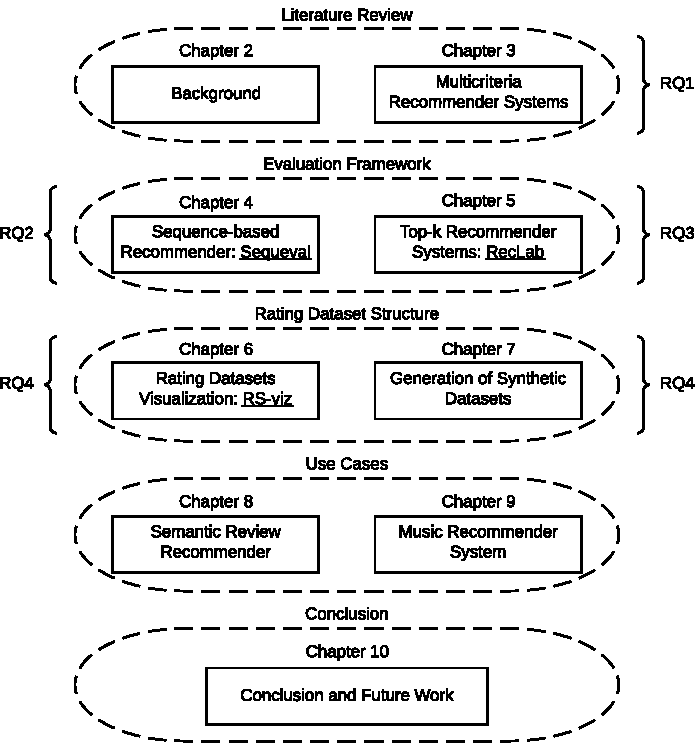
\includegraphics[width=\textwidth]{structure}
\caption[Overview of the dissertation structure]{\added{An overview of the dissertation structure illustrating its division in chapters, the top-level research questions and the main outcomes of the related research activity. The software tools developed are underlined.}}
\label{int:fig:structure}
\end{figure}

In summary, \added{as depicted in Figure~\ref{int:fig:structure},} this dissertation deals with the problem of conducting an offline comparison of recommender systems from different perspectives. We analyze existing approaches for exploiting multicriteria ratings, with a special emphasis on the methods currently employed for validating the quality of the suggestions. Then, we discuss multicriteria evaluation techniques, considering both sequence-based recommenders as well as more traditional approaches. Furthermore, we explore the problem of selecting the right dataset according to the evaluation context by visualizing its structure and generating alternative versions of it. Finally, we apply our knowledge of multicriteria evaluation techniques to different use cases. We propose and evaluate with an ensemble of metrics a semantic review recommender capable of annotating product reviews to extract useful information from them and a music recommender system designed to create playlists starting from a few songs that represent the seeds of the process.

The remainder of this dissertation is organized as follows. In Chapter~\ref{chap:background}, we review existing recommendation and evaluation approaches available in literature and the associated challenges. In Chapter~\ref{chap:multicriteria}, we report the results of a systematic literature review dealing with the topic of multicriteria recommender systems. In Chapter~\ref{chap:sequeval}, we introduce Sequeval, our framework for evaluating sequence-based recommender systems, while, in Chapter~\ref{chap:reclab}, we discuss RecLab, a Web-based evaluation toolkit for top-$k$ recommenders. In Chapter~\ref{chap:rs-viz}, we describe a qualitative method for visualizing the ratings available in any collection of users' preferences. In Chapter~\ref{chap:synthetic}, we present our approach for generating a synthetic dataset that exhibits the same properties of a real one. In Chapter~\ref{chap:semrevrec}, we report on the creation and evaluation of a semantic review recommender, while, in Chapter~\ref{chap:challenge}, we describe our approach for automatically generating music playlists. Finally, in Chapter~\ref{chap:conclusion}, we formulate our conclusions and we discuss open issues and possible future works.

\chapter{Background}
\label{chap:background}

Nowadays, the amount of information available on the Web is overwhelming. For this reason, the availability of tools capable of selecting from a huge catalog a short list of items that are of potential interest for a particular user is a critical success factor for almost any online platform. Therefore, recommender systems represent one of the technical solutions commonly employed in industry to address the issue of effectively exploring a vast horizon of possible choices.

A related and equally popular approach is represented by search engines. Despite the common roots of these solutions, the task of evaluating with an offline experiment a recommender system is usually more challenging, as the ground truth is represented by subjective, and sometimes even emotional, preferences.

In this chapter, we first review some of the recommendation approaches available in literature (Section~\ref{soa:sec:recommender}), then we discuss the main challenges associated with their offline evaluation (Section~\ref{soa:sec:evaluation}).

\section{Recommender Systems}
\label{soa:sec:recommender}

According to Ricci et al.~\cite{Ricci2015}, recommender systems are software tools and algorithms designed to suggest items to users according to their preferences.

In general, recommender systems can be classified in different categories based on the recommendation approach. The most widespread categories of recommender systems are content-based, collaborative filtering, knowledge-based, and hybrid~\cite{Adomavicius2005}, \added{as summarized in Table~\ref{soa:tab:methods}}. Content-based recommenders only rely on the past preferences of the current user in order to construct her profile and select suggested items. In contrast, collaborative filtering approaches analyze the behaviour of similar users for identifying candidate items. A knowledge-based recommender embeds domain-specific knowledge that is used for matching user requirements with items of potential interest. Finally, hybrid approaches combine in many different ways the previous methods. Other less common categories of recommender systems include community-based and demographic techniques~\cite{Burke2007}. A community-based recommender also considers the relationships of trust among its users, while a demographic recommender mainly relies on demographic profiles.

\begin{table}
\centering
\begin{tabular}{@{}lp{4cm}p{4cm}@{}}
\toprule
Method & Advantages & Disadvantages \\ \midrule
Content-based & Transparency, limited privacy issues & Requires a description of the items \\
Collaborative filtering & Scalability, only based on ratings & Data sparsity and cold start problems \\
Knowledge-based & No interaction history required & Difficult to the create the model \\
Hybrid & Combines multiple approaches together & Limited performance \\ \bottomrule
\end{tabular}
\caption[Comparison of recommendation techniques]{\added{Comparison of the advantages and disadvantages of the recommendation techniques mentioned in~\cite{Adomavicius2005}.}}
\label{soa:tab:methods}
\end{table}

A detailed analysis of the recommendation approaches available in literature is beyond the scope of this dissertation. Many authors already conducted different studies dealing with the topic of recommender systems. Park et al.~\cite{Park2012} reviewed hundreds of journal articles for analyzing the main application fields and data mining techniques exploited by different recommenders. Hong et al.~\cite{Hong2009} discussed the literature about context-aware recommenders, while Figueroa et al.~\cite{Figueroa2015} and Çano et al.~\cite{Cano2017} conducted systematic literature reviews about Linked Data and hybrid recommender systems respectively.

More recently, Quadrana et al.~\cite{Quadrana2018} classified different approaches according to their capability of managing sequences of items. Portugal et al.~\cite{Portugal2018} reviewed commonly exploited machine learning techniques, while Zhang et al.~\cite{Zhang2019} discussed the most promising deep learning methods for generating personalized items.

In the following, we briefly introduce a formal definition of the recommendation problem. Then, we review the recommendation approaches considered in this dissertation, that is \added{top-$k$,} sequential, review-based, and Linked Data-based ones. \added{Please note that sequence-based recommender systems are a generalization of sequential recommenders and they will be defined later in Section~\ref{seq:sec:sequence-based}.}

\subsection{Top-k Recommender Systems}
\label{soa:sec:topk}

Traditionally, recommender systems try to identify for each user an item that maximises the utility that she should gain from the consumption of that item~\cite{Bobadilla2013}. In other words, recommender systems estimate a utility function $R(\upsilon, \iota)$ that, given a user $\upsilon \in \mathcal{U}$ and an item $\iota \in \mathcal{I}$, predicts if $\iota$ should be recommended to $\upsilon$. In principle, the utility function could be an arbitrary function, including a profit function. The formal definition of this problem, as provided by Adomavicius \& Tuzhilin~\cite{Adomavicius2015}, is reported in Equation~\ref{soa:eq:utility}.

\begin{equation}
\forall \upsilon \in \mathcal{U}, \quad \iota^{\prime}_{\upsilon} = \arg \max \limits_{\iota \in \mathcal{I}} R(\upsilon, \iota)
\label{soa:eq:utility}
\end{equation}

In practice, users are commonly asked to quantify their preferences with numerical values, called ratings. For example, ratings could be the number of stars assigned to a product or the indication if they liked or not a movie. Therefore, the utility function $R$ is used by the system to calculate the ratings that users would probably assign to unknown items. Such a value measures the appropriateness of recommending an item to a certain user.

The ratings already available can be represented as a matrix, similar to the one illustrated in Table~\ref{soa:tab:ratings}. In real systems, this matrix should be sparse, because the number of unknown cells is usually extremely elevated~\cite{Ricci2015}. In fact, users can provide ratings on a limited set of items, especially if the catalog is very large.

\begin{table}
\centering
\begin{tabular}{@{}lccccc@{}}
\toprule
& \texttt{Item\_1} & \texttt{Item\_2} & \texttt{Item\_3} & \texttt{Item\_4} & \texttt{Item\_5} \\ \midrule
\texttt{User\_1} & \texttt{5} & \texttt{3} & \texttt{4} & \texttt{4} & \texttt{?} \\
\texttt{User\_2} & \texttt{?} & \texttt{1} & \texttt{?} & \texttt{3} & \texttt{3} \\
\texttt{User\_3} & \texttt{4} & \texttt{3} & \texttt{?} & \texttt{?} & \texttt{5} \\
\texttt{User\_4} & \texttt{3} & \texttt{?} & \texttt{1} & \texttt{?} & \texttt{?} \\
\texttt{User\_5} & \texttt{?} & \texttt{5} & \texttt{5} & \texttt{2} & \texttt{1} \\ \bottomrule
\end{tabular}
\caption[Example of rating matrix]{An example of rating matrix. Unknown ratings are denoted with an interrogative mark.}
\label{soa:tab:ratings}
\end{table}

Different approaches can be exploited to compute unknown ratings. For example, in a collaborative filtering setting, popular techniques include user-based or item-based \textit{k}-NN and matrix factorization methods~\cite{Jannach2010}.

Even if the recommendation problem \added{is traditionally formalized as} the task of predicting unknown ratings, many commercial systems provide to each user a ranked list of suggestions~\cite{Lu2015}. \added{Therefore, a recommender system capable of selecting $k$ items per user can be defined as a top-$k$ recommender.} It is straightforward to obtain a top-$k$ list starting from the predicted ratings, as it is sufficient to sort them and select only the items with the highest computed values~\cite{Adomavicius2015}.

\subsection{Sequential Recommender Systems}
\label{soa:sec:sequential}

A recommender system designed to consider the timestamp associated to user ratings can be defined as a sequential recommender~\cite{Quadrana2018}. In the following, we review some examples of sequential recommenders available in literature.

Zhou et al.~\cite{Zhou2004} proposed a web recommender system based on a sequential pattern mining algorithm. The recommender is trained with the access logs of a website and its goal is to predict the pages that are likely to be visited by a certain user, given her previously visited pages. The authors proposed to store the model in a tree-like structure, relying on a technique originally designed for matching substrings over a finite alphabet of characters. A recommendation is then created by matching the sequence of pages already visited by the target user with the sequences previously analyzed by the algorithm.

In the context of market basket analysis, it is also possible to exploit the sequence of previous transactions to predict what a customer is going to buy next~\cite{Aggarwal2015}. Rendle et al.~\cite{Rendle2010} proposed a method based on personalized transition graphs over Markov chains, while Wang et al.~\cite{Wang2015} designed a recommender capable of modeling both the sequential information from previous purchases and the overall preferences by a hybrid representation.

Bellog\'in and S\'anchez~\cite{Bellogin2017a} proposed a similarity metric designed to compare users in the context of CF recommender systems. This metric takes into account the temporal sequence of users' ratings to identify common behaviors. The authors argue that it is possible to consider a sequence of items as a string, where each character represents an item, and compare them using the longest common subsequence algorithm~\cite{Hirschberg1975}.

More recently, He et al.~\cite{He2017} introduced the concept of \emph{translation-based} recommendation. While a traditional recommender only considers the pairwise interactions between items and users, their idea is to model a third-order relationship among a user, the items she interacted with in the past, and the item she is going to visit next. Each user can be represented as a vector in a transition space: given the current item, it is possible to compute where the next one will be located. At recommendation time, it is possible to generate a list of suggested items by relying on a nearest-neighbor search.

On the other hand, the task of generating recommendations of sequences was already discussed and presented in a seminal work by Herlocker et al.~\cite{Herlocker2004}. The authors suggested that it would be intriguing to be able to suggest, in the music domain, not only the songs that will be probably liked by a certain user, but also a playlist of songs that is globally pleasing. Moreover, they also proposed to apply this recommendation methodology in the context of scientific literature, where it is necessary to read a sequence of articles to become familiar with a certain topic.

% Playlist recommendation
The problem of recommending music songs was later addressed by Chen et al.~\cite{Chen2012}, who designed and implemented a recommender system capable of generating personalized playlists by modeling them as Markov chains. Their algorithm is capable of learning, from a set of training playlists, how to represent each song as a point in a latent space. Then, starting from a seed song, it is possible to create a playlist of an arbitrary length by repeatedly sampling the transition probabilities between adjacent songs. The resulting playlist is personalized because of the chosen seed. Furthermore, each user can influence the generation process by specifying some parameters: for example, a user might be more interested in popular songs, while another one in songs that are strictly related to the given seed.

% Next POI recommendation
Another typical application for a sequence-based recommender is the \emph{next} point-of-interest (POI) prediction problem~\cite{Quadrana2018}. Given some training sequences of previously liked geographical locations, this task consists of predicting a sequence of venues that is pleasing for a given user. Feng et al.~\cite{Feng2015} proposed an algorithm capable of creating sequences of POIs that have not been already visited. The authors developed a Metric Embedding algorithm that captures both the sequential information and individual preference. Such metric is then exploited to create a Markov chain model capable of representing the transition probabilities between a given POI and the next one. The key features that are implicitly considered in the embedding creation phase are the conceptual similarity and the geographical distance of the analyzed venues.

A different line of research is represented by recommenders capable of analyzing sequences of multimedia objects. For example, Albanese et al.~\cite{Albanese2010} proposed a hybrid recommender system for retrieving multimedia content based on the theory of social choice and capable of exploiting, among other signals, the implicit browsing preferences of its users. Later, the authors of~\cite{Albanese2013} introduced a multimedia recommendation algorithm capable of combining semantic descriptors and usage patterns. The proposed approach can manage different media types and it enables users to explore several multimedia channels at the same time. Possible applications of such technologies are represented by browsing tools for virtual museums~\cite{Amato2017} and recommenders of cultural heritage sites~\cite{Su2019}.

\subsection{Review-based Recommender Systems}
\label{soa:sec:review-rs}

The exploitation of user reviews in recommender systems is a well-known research topic, as reported by Cheng et al.~\cite{Chen2015}. Some techniques try to tackle the problem of building the profile of users by analyzing their reviews, while others focus on the identification of the main features of the items to recommend.

Different strategies have been proposed in the literature to address the latter problem. Some researchers have suggested methods able to identify the sentiment associated with the features of an item exploiting a domain-specific ontology~\cite{Aciar2007} or its technical description~\cite{Yates2008}. A common aspect of these techniques is that the possible features are already available before performing the analysis. However, in literature there are also approaches for unsupervised extraction of product features and sentiment from reviews~\cite{Qiu2011, Somprasertsri2010}.

Another possibility is to identify the main characteristics of an item with the help of natural language processing methods, without any previous knowledge of the context. For example, a popular technique considers bigrams that frequently occur in reviews and that are associated with a word expressing an emotion~\cite{Dong2013}. In this case, the goal of the recommender system is suggesting items with the same features of the ones liked by the target user, but with a better global sentiment. In the best of our knowledge, there is only one attempt to exploit user reviews for recommendation tasks using semantic annotation. Dzikowski et al.~\cite{Dzikowski2012} applied semantic annotation to reviews while users are editing them. Their goal was to produce annotated reviews of restaurants through Linked Data in order to generate tags to be associated with the reviewed items.

\subsection{Linked Data-based Recommender Systems}
\label{soa:sec:linked-data}

In the past, some studies reviewed different Linked Data-based recommender systems that were proposed in literature~\cite{DiNoia2015, Figueroa2015}. Typically, these recommender systems consider the relationships among resources by taking into account the existing links in the Web of Data and use them to measure a semantic similarity. Such relationships can be direct links or paths between the items to recommend. In the following, we summarize the main works in this field. 

Damljanovic et al.~\cite{Damljanovic2012} suggested domain experts in an open innovation scenario. Their approach generates recommendations by discovering related resources through hierarchical or transversal relationships in DBpedia. Passant~\cite{Passant2010} presented \emph{dbrec}, a music recommender system, which mainly relies on a measure named Linked Data Semantic Distance (LDSD). This measure is based on the number of direct and indirect links between two resources. Heitmann and Hayes~\cite{Heitmann2010} also proposed a recommender system which exploited Linked Data to mitigate the new-user, new-item and sparsity problems of collaborative recommender systems.

More recently, Musto et al.~\cite{Musto2016} studied the impact of the knowledge available in the Web of Data on the overall performance of a graph-based recommendation algorithm. Vagliano et al.~\cite{Vagliano2016} presented a recommendation algorithm based on Linked Data which exploits existing relationships between resources by dynamically analyzing both their categories and their explicit references to other resources. Di Noia et al.~\cite{DiNoia2012} described a model-based approach to provide content-based recommendations with Linked Data. Ostuni et al.~\cite{Ostuni2014} defined a neighborhood-based graph kernel for matching graph-based item representations. Di Noia et al.~\cite{DiNoia2016} introduced SPrank, a hybrid algorithm which extracts semantic path-based features from DBpedia and computes recommendations using Learning to Rank.

\section{Offline Evaluation}
\label{soa:sec:evaluation}

To the best of our knowledge, the first survey that deals with the problem of evaluating a recommender system was conducted by Herlocker et al.~\cite{Herlocker2004}. In their work, the authors discuss when it is appropriate to perform an offline evaluation and when it is necessary to carry on an online, or in~vivo, experiment. The former is particularly useful to select a small set of potentially good candidates that will be further compared in a real scenario. However, to be complete and trustworthy, such an evaluation needs to rely on a set of well-defined metrics, that should be able to capture all characteristics of the recommended items.

\added{An offline analysis is an experimental approach based on user preferences collected before the introduction of the system under evaluation. Therefore, it is a simple and effective method to conduct large scale evaluations, usually considering different algorithms and datasets. Its major requirement is the availability of a collection of user preferences in the domain of interest. If the dataset at disposal also includes timestamps, it is possible to exploit it considering ratings and recommendations according to their temporal order. However, offline evaluations are based on datasets that are usually sparse: for this reason, it is not possible to reliably evaluate recommendations that involve items with no ratings available from the target user. Furthermore, offline experiments based on existing rating datasets cannot consider other important factors such as the usability of the user interface. An alternative approach is represented by live experiments. They can be classified as user studies when they are conducted in a controlled environment with a limited set of subjects, or as online analyses when a recommender system is made available to a potentially large community of users.}

In the following, we introduce the problem of experimental reproducibility, then we explain why it is necessary to consider a multicriteria set of metrics for conducting a reliable evaluation. Finally, we review existing visualization and generative approaches in the context of rating datasets.

\subsection{Experimental Reproducibility}

Different authors analyzed the experimental reproducibility of offline evaluations in the context of recommender systems. For example, Jannach et al.~\cite{Jannach2015} compared several recommendation algorithms in an offline experiment, analyzing their performance by relying on a comprehensive evaluation framework. The authors considered different splitting protocols and metrics, designed to characterize both the accuracy, in terms of rating and ranking, and the coverage of the suggested items. The results of the experimental trails suggest that some common algorithms, despite their high accuracy, tend to only recommend popular items that are probably not very interesting for the users of a real system. This problem is related to the popularity biases introduced by the offline evaluation protocol: for this reason, it is not advisable to compare different algorithms by relying only on measures related to their accuracy. In addition, different splitting protocols produce significantly different and non-comparable outcomes.

Gunawardana and Shani~\cite{Gunawardana2015} proposed a set of general guidelines for designing experiments with the purpose of evaluating recommender systems. Such experiments can be classified as offline trails, user studies, or online analysis that involve a live system. Several properties of a recommender system can be evaluated: for example, the most common ones are user preference, prediction accuracy, coverage, and utility. The authors argue that the possibility of measuring these properties is strongly influenced by the kind of study and, in the most extreme scenario, some of them cannot be obtained. For example, it is very difficult to measure users' preference in an offline setting.

For each property, different commonly exploited metrics are presented and discussed. Even if the main metrics proposed for evaluating the most popular properties are widely known and understood, usually there is little agreement about the most appropriate metrics for characterizing the least common properties. For example, several definitions, and several metrics, related to the property of utility are available in the literature. The authors also point out that a key decision of offline experiment design is the splitting protocol because this choice will greatly influence the final outcome of the measures.

Bellog\'in et al.~\cite{Bellogin2017} proposed an evaluation framework designed following the methodologies of the information retrieval field. They suggest that the evaluation procedures available in information retrieval are widespread: for this reason, they could be successfully exploited by the recommender systems community to create a shared evaluation protocol based on ranking, as this setting is more similar to the one of a live system. Unfortunately, three different design decisions need to be taken to achieve this goal.

The items considered for the evaluation could be all items available in the dataset, or only the items available in the test set. The non-relevant items for a certain user could be represented by all items in the test set not rated by that user, or by a subset of it with a fixed size. Finally, the global metric could be computed by averaging its value on all users, or on all ratings available in the test set. Different design choices will result in different evaluation protocols and results. The authors also identify two sources of biases in offline evaluations protocols: the sparsity bias and the popularity bias.

Several software tools are available with the purpose of simplifying the process of comparing the performance of recommendation algorithms. They typically include some evaluation protocols and a reference implementation of well-known techniques. Said and Bellog\'in~\cite{Said2014} compared several of these tools to check if their results are consistent. They discovered that the values obtained with the same dataset and algorithm may vary significantly among different frameworks. For this reason, it is not feasible to directly compare the scores reported by these tools, because they are obtained relying on several protocols. The discrepancies reported by the authors are mainly caused by the data splitting protocol, the strategy used to generate the candidate items, and the implementation choices related to the evaluation metrics.

\subsection{Beyond Accuracy}
\label{soa:sec:beyond}

In their survey dealing with the problem of evaluating a recommender system, Herlocker et al.~\cite{Herlocker2004} review several accuracy metrics usually exploited by different authors and they classify them into three categories: predictive accuracy metrics, classification accuracy metrics, and rank accuracy metrics. These groups are strictly related to the purpose of the recommender system: predicting a rating for each user-item pair, identifying an item as appropriate or not for a user, and creating an ordered list of recommended items for a user. After discussing the accuracy-based metrics, they argue that, in order to draw a reliable conclusion, it is necessary to also consider other properties of the recommended items. In their opinion, a recommender system should be capable of providing suggestions that are not only accurate but also useful. For example, an extremely popular item may be an accurate but not an interesting suggestion. For this reason, they also discuss other metrics that could be considered beyond the traditional concept of accuracy, such as coverage, learning rate, novelty, serendipity, and confidence.

The idea of relying not only on accuracy-based metrics is also supported by Ge et al.~\cite{Ge2010}. In their work, the authors state that the purpose of an evaluation protocol is to assess the quality of the recommended items and not their accuracy. However, metrics like precision and recall alone are not capable of verifying that the recommendations are actually useful. In fact, only the users of the system can judge their quality in the context of an online experiment. Therefore, their suggestion is to consider a multicriteria set of metrics and not only accuracy when it is necessary to perform an offline study.

\subsection{Visualization Approaches}

Different authors have proposed to create interactive visualizations for qualitative evaluating the goodness of the recommended items or helping the users to identify the most relevant suggestions. For example, Kunkel et al.~\cite{Kunkel2017} created a 3D map-based visualization that represents the preferences of a user on the entire space of items. The user can inspect the profile created by the recommender and also manually modify it, if necessary.

\c{C}oba et al.~\cite{Coba2017} extended the \textit{rrecsys} library by adding to it graphical capabilities for performing an offline visual evaluation of different recommendation approaches with respect to the popularity of the suggested items. Gil et al.~\cite{Gil2018} introduced VisualRS, a tool capable of creating tree graph structures for exploring the most important relationships between items or users. The graph-based visualization is useful for comparing the results of different recommendation approaches and selecting the most appropriate one for a given task. In contrast, Cardoso et al.~\cite{Cardoso2019} proposed to combine the output of different recommender systems with human-generated data to allow users to explore the suggested items in an effective way. This method could also be exploited to compare the results of different recommender systems in a qualitative way.

\subsection{Synthetic Datasets}

Synthetic datasets are commonly used in literature to assess the performance of database systems or to study the behavior of data mining algorithms. For example, Agrawal et al.~\cite{Agrawal1994} created a generator of retail transactions intended for the evaluation of association rule algorithms, while Houkj{\ae}r et al.~\cite{Houkjaer2006} introduced a software capable of creating relational data for benchmarking purposes. Such tools can generate realistic data in terms of their statistical distributions, which can be empirically learned for existing datasets or provided by a researcher using domain-specific languages.

Similar approaches have been also explored in the field of recommender systems, usually because of the lack of public datasets with the required characteristics. Tso et al.~\cite{Tso2006} created a synthetic data generator for evaluating context-aware recommenders based on Dirichlet and Chi-square distributions. The metric of information entropy is then exploited to control the randomness of the synthetic data. A similar method has been discussed by Pasinato et al.~\cite{Pasinato2013}: their intuition is to represent the heterogeneous rating behaviors of the users with different statistical distributions.

Manouselis et al.~\cite{Manouselis2008} presented a tool, named CollaFis, capable of creating synthetic ratings for the evaluation of either single-criteria or multi-criteria recommender systems. The users of CollaFis need to specify the characteristics of the generated data, like the number of users, items, and criteria. A common aspect of all the previously mentioned methods is that researchers are required to choose and configure the statistical distributions that are exploited to generate the artificial datasets. However, the main problem of such an approach is that it is impossible to predict the real behavior of many different users with a few statistical distributions~\cite{Montaner2004}.

Another possible line of research is related to the imitation of a real collection of preferences. For example, Rodr{\'i}guez-Hern{\'a}ndez et al.~\cite{CarmenRodriguez-Hernandez2017} developed a software, DataGenCARS, for creating artificial ratings using a set of parameters provided by the user or inferred from a reference dataset. However, in Chapter~\ref{chap:synthetic}, we argue that statistics computed at a global level are not informative enough to create a synthetic dataset, as they are not able to capture the different behaviors of the various groups of users.

\chapter{Multicriteria Recommender Systems}
\graphicspath{{Chapter03/Figures/}}
\label{chap:multicriteria}

The traditional approach to the recommendation problem discussed in Section~\ref{soa:sec:recommender} could be considered somewhat limited, as users typically tends to judge items according to different criteria~\cite{Adomavicius2015}. For example, we can easily imagine to assign different ratings to a movie, expressing how much we liked the story, the acting, the direction, and the visual effects. Such multiple ratings could be exploited by a recommender system in order to identify more effectively which items should be suggested. For this reason, different authors started to propose multicriteria recommender systems, namely methods capable of suggesting items by relying on ratings provided over different criteria instead of a single one~\cite{Adomavicius2005,Manouselis2007}.

In this chapter, we investigate the state of the art in the field of multicriteria recommender systems. We follow the systematic literature review protocol proposed by Kitchenham \& Charters~\cite{Kitchenham07}, in order to enable other researchers to easily verify and reproduce our work. We consider nine different research questions that encompass various aspects of the reviewed studies.

In particular, we analyze the most important problems that multicriteria recommenders aim to address, as well as the exploited recommendation approaches, according to the taxonomy created by Burke~\cite{Burke2007}. We also describe the different machine learning and data mining techniques typically included in a multicriteria recommender and we identify which methods are frequently utilized in each recommendation phase, thus we try to describe the structure of an ideal multicriteria RS. We quantitatively measure the domains that are the most appropriate ones for such systems and we review how the proposed algorithms have been evaluated with respect to the experimental settings, the metrics, and the exploited datasets. Finally, we describe the most promising directions for future works that are mentioned in the reviewed studies.

We considered a total number of 93 studies, published from 2003 to 2018, to perform this systematic literature review. To the best of our knowledge, this is the first review conducted in the field of multicriteria recommender systems that follows a standardized and repeatable protocol. We aim that our study could be useful to other researchers working in this area, especially for better identifying possible approaches and future trends.

The remainder of this chapter is structured as follows. In Section~\ref{mcr:sec:methodology}, we detail the protocol that we followed for conducting the review. Then, we present the quantitative results in Section~\ref{mcr:sec:results} and we provide a possible interpretation of the outcomes of the review in Section~\ref{mcr:sec:discussion}. Finally, we conclude this chapter with Section~\ref{mcr:sec:conclusions}, while, in Appendix~\ref{chap:studies-slr}, we report the list of selected studies.

\section{Methodology}
\label{mcr:sec:methodology}

We decided to perform this review according to the guidelines designed by Kitchenham \& Charters for Systematic Literature Reviews (SLR) in the field of Software Engineering~\cite{Kitchenham07}. This method guarantees that the outcome of the review is verifiable and repeatable by other researches. The protocol, which is graphically illustrated in Figure~\ref{mcr:fig:protocol}, was developed by the author of this dissertation.

\begin{figure}
\centering
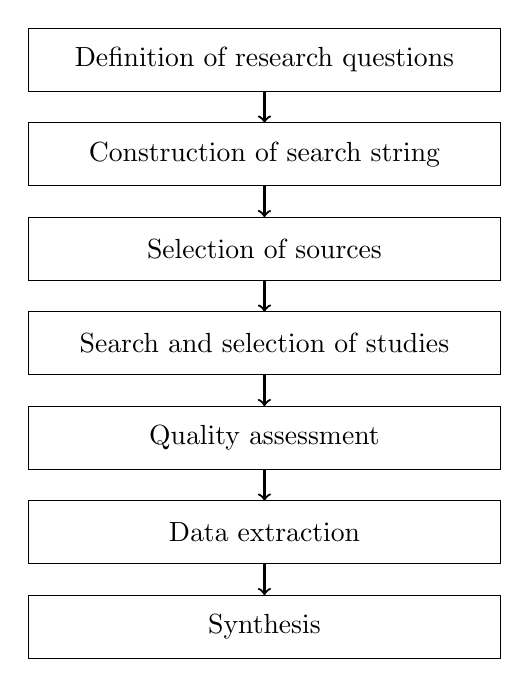
\begin{tikzpicture}
\draw (0,0) rectangle (6,-0.8);
\draw (3,-0.4) node {Definition of research questions};
\draw[thick,->] (3,-0.8) -- (3,-1.2);
\draw (0,-1.2) rectangle (6,-2);
\draw (3,-1.6) node {Construction of search string};
\draw[thick,->] (3,-2) -- (3,-2.4);
\draw (0,-2.4) rectangle (6,-3.2);
\draw (3,-2.8) node {Selection of sources};
\draw[thick,->] (3,-3.2) -- (3,-3.6);
\draw (0,-3.6) rectangle (6,-4.4);
\draw (3,-4) node {Search and selection of studies};
\draw[thick,->] (3,-4.4) -- (3,-4.8);
\draw (0,-4.8) rectangle (6,-5.6);
\draw (3,-5.2) node {Quality assessment};
\draw[thick,->] (3,-5.6) -- (3,-6);
\draw (0,-6) rectangle (6,-6.8);
\draw (3,-6.4) node {Data extraction};
\draw[thick,->] (3,-6.8) -- (3,-7.2);
\draw (0,-7.2) rectangle (6,-8);
\draw (3,-7.6) node {Synthesis};
\end{tikzpicture}
\caption[Systematic literature review protocol]{The systematic literature review protocol designed following the guidelines by Kitchenham \& Charters~\cite{Kitchenham07}.}
\label{mcr:fig:protocol}
\end{figure}

\subsection{Research Questions and Search String}
\label{mcr:sec:questions}

The purpose of this systematic literature review is to identify the studies describing multicriteria recommender systems and to understand the motivations behind their usage, the techniques employed, the experimental protocols used to validate them, and the related research challenges. For these reasons, we defined the following research questions.

\begin{description}
\item[RQ1.1\label{mcr:itm:rq1}] What are the most relevant studies addressing multicriteria RSs?
\item[RQ1.2\label{mcr:itm:rq2}] What are the most challenging problems faced by researchers?
\item[RQ1.3\label{mcr:itm:rq3}] What are the approaches used by multicriteria recommenders?
\item[RQ1.4\label{mcr:itm:rq4}] Which techniques and methods have been proposed?
\item[RQ1.5\label{mcr:itm:rq5}] In which domains multicriteria recommender systems are applied?
\item[RQ1.6\label{mcr:itm:rq6}] Which protocols and frameworks are used for their evaluation?
\item[RQ1.7\label{mcr:itm:rq7}] Which metrics are considered during their evaluation?
\item[RQ1.8\label{mcr:itm:rq8}] Which datasets are used for testing the algorithms?
\item[RQ1.9\label{mcr:itm:rq9}] What are the most promising directions for future works?
\end{description}

In order to retrieve the studies related to multicriteria recommender systems, we defined the following preliminary set of keywords: \{Multicriteria, Recommender System\}. This initial set was expanded to include alternative spellings and we defined the search string used to query the digital sources as follows.

\begin{lstlisting}
(multicriteria OR "multi criteria" OR "multi-criteria") AND ("recommender system" OR "recommendation system")
\end{lstlisting}

We selected six scientific digital libraries that contain primary studies related to the field of computer science, as detailed in Table~\ref{mcr:tab:sources}. Other more general sources, like Google Scholar, were not included because they usually index studies already available in the primary sources.

\begin{table}
\centering
\begin{tabular}{@{}ll@{}}
\toprule
Source               & URL                                 \\ \midrule
ACM Digital Library  & \url{https://dl.acm.org}            \\
IEEE Xplore          & \url{http://ieeexplore.ieee.org}    \\
ISI Web of Knowledge & \url{http://www.webofknowledge.com} \\
ScienceDirect        & \url{https://www.sciencedirect.com} \\
Scopus               & \url{https://www.scopus.com}        \\
Springer Link        & \url{https://link.springer.com}     \\ \bottomrule
\end{tabular}
\caption[Digital libraries considered]{The digital libraries considered during the search process.}
\label{mcr:tab:sources}
\end{table}

\subsection{Selection Process}

The selection process \added{was performed} during January 2019. We inserted the search query in the search field of the digital libraries selected as sources for the review and we retrieved all the studies identified by the respective search engines. \added{Because of the high number of false positive results, we decided to limit our search to the title, abstract, and keywords with IEEE Xplore, ISI Web of Knowledge, and Scopus.} The preliminary set \added{initially contained} $1256$ studies. We checked their titles and authors in order to discover possible duplicates: after having removed duplicated results, the preliminary set \added{was reduced} to $950$ studies.

Furthermore, for objectively identifying the studies to include in the review, we defined a set of inclusion and exclusion criteria, which are summarized in Table~\ref{mcr:tab:criteria}. We first applied the criteria in a coarse selection phase by only considering their abstracts and we obtained a list of $301$ papers. Then, we analyzed again the available studies in a detailed selection phase by reading relevant portions of their content. We finally selected $93$ studies as part of this literature review, as summarized in Table~\ref{mcr:tab:numbers}. The full list, \added{sorted by source, year of publication and author,} is available in Appendix~\ref{chap:studies-slr}.

\begin{table}
\centering
\begin{tabular}{@{}ll@{}}
\toprule
Code & Inclusion criteria \\ \midrule
IC1 & Papers describing multicriteria recommender systems \\
IC2 & Papers published in conferences and journals \\
IC3 & Papers written in English language \\ \midrule
Code & Exclusion criteria \\ \midrule
EC1 & Papers not addressing recommender systems \\
EC2 & Papers addressing RSs without multicriteria ratings \\
EC3 & Papers that report only abstracts or posters \\
EC4 & Papers that describe a planned research\footnotemark \\
EC5 & Grey literature and book chapters \\ \bottomrule
\end{tabular}
\caption[Inclusion and exclusion criteria]{The inclusion and exclusion criteria.}
\label{mcr:tab:criteria}
\end{table}
\footnotetext{\added{We defined a planned research as a study that only contains a high level description of the proposed methodology, without the details necessary to implement it.}}

\begin{table}
\centering
\begin{tabular}{@{}llll@{}}
\toprule
Source               & Search & Coarse & Detailed \\ \midrule
ACM Digital Library  & 27     & 24     & 11       \\
IEEE Xplore          & 38     & 36     & 15       \\
ISI Web of Knowledge & 31     & 25     & 6        \\
ScienceDirect        & 344    & 81     & 19       \\
Scopus               & 118    & 62     & 24       \\
Springer Link        & 392    & 73     & 18       \\ \midrule
Total                & 950    & 301    & 93       \\ \bottomrule
\end{tabular}
\caption[Studies per selection step]{The number of studies after each selection step.}
\label{mcr:tab:numbers}
\end{table}

\subsection{Quality Assessment}

For objectively assessing the quality of the studies selected as part of this review, we defined eight quality questions, as listed in Table~\ref{mcr:tab:quality}. It is possible to assign to each question the scores of $0$, $0.5$, and $1$, that correspond, respectively, to the answers \emph{Yes}, \emph{Partly}, and \emph{No}. During the quality assessment phase, we provided an answer to each question for all studies included in the review.
 
\begin{table}
\centering
\begin{tabular}{@{}ll@{}}
\toprule
Code & Quality question \\ \midrule
QQ1 & Did the study clearly describe the problems that it is addressing? \\
QQ2 & Did the study review the related work for the problem? \\
QQ3 & Did the study compare its approach with possible alternatives? \\
QQ4 & Did the study describe the components of the proposed RS? \\
QQ5 & Did the study provide an empirical evaluation of the solution? \\
QQ6 & Did the study present a clear statement of the findings? \\
QQ7 & Did the study analyze the application scenarios of the RS? \\
QQ8 & Did the study recommend any further research activity? \\ \bottomrule
\end{tabular}
\caption[Quality questions]{The quality questions.}
\label{mcr:tab:quality}
\end{table}

\subsection{Data Extraction}

We carefully read multiple times the primary studies \added{that are} selected as part of this review. During this phase, we identified the data available in the works useful for providing an answer to the research questions introduced in Section~\ref{mcr:sec:questions}. More in details, we looked for the information listed in Table~\ref{mcr:tab:form}. This process was supported by the data analysis software tool NVivo.\footnote{\url{https://www.qsrinternational.com/nvivo}} \added{We relied on this tool to minimize the manual effort required for applying the methodology described in Section~\ref{mcr:sec:synthesis}.}

\begin{table}
\centering
\begin{tabular}{@{}lll@{}}
\toprule
Field & Description & RQ  \\ \midrule
Code & An internal identifier of the study & - \\
Title & - & \ref{mcr:itm:rq1} \\
Authors & - & - \\
Publication year & - & \ref{mcr:itm:rq1} \\
Publication name & - & - \\
Source & The digital library that contains the study & - \\
Type & Conference or journal & - \\
DOI & - & - \\
Research problem & The problem that the study tries to address & \ref{mcr:itm:rq2} \\
Contribution & The description of the proposed method & \ref{mcr:itm:rq3} \\
Implementation & How the method was implemented & \ref{mcr:itm:rq4} \\
Domain & The domain of the recommended items & \ref{mcr:itm:rq5} \\
Evaluation protocol & The protocol used to evaluate the method & \ref{mcr:itm:rq6} \\
Evaluation metric & The metric used to compare the RS & \ref{mcr:itm:rq7} \\
Dataset & The dataset used to execute the evaluation & \ref{mcr:itm:rq8} \\
Limitation & The limitations of the proposed method & \ref{mcr:itm:rq9} \\
Future work & The suggestions for future works & \ref{mcr:itm:rq9} \\
Quality score & - & - \\ \bottomrule
\end{tabular}
\caption[Data extraction form]{The data extraction form.}
\label{mcr:tab:form}
\end{table}

\subsection{Synthesis}
\label{mcr:sec:synthesis}

We synthesized the results of our review following the Cruzes \& Dyba methodology~\cite{Cruzes2011} for combining and comparing the results of the primary studies that we considered. While reading the selected studies, we associated relevant portions of their text with codes. A code is a label applied to text segments that discuss the same theoretical or descriptive idea and that is used to aggregate in an organic way the data that we are analyzing. We initially defined some general codes associated with the research questions. Then, we created more specialized sub-codes related to the content of the studies, thus following an integrated approach that combines both inductive and deductive methods and that is considered the most appropriate one for a systematic review~\cite{Cruzes2011}. We subsequently aggregated the codes in themes, and we mapped these themes back to the original research questions. The outcomes of this last phase are reported in Section~\ref{mcr:sec:results}, grouped by research question.

\section{Results}
\label{mcr:sec:results}

In this section, we highlight the findings of our systematic literature review regarding multicriteria recommender systems, according to the research questions introduced in Section~\ref{mcr:sec:questions}. These results will be further discussed in Section~\ref{mcr:sec:discussion}.

\subsection{Included Studies}
\label{mcr:sec:included}

The main purpose of \ref{mcr:itm:rq1} is to identify the studies related to the topic of multicriteria recommender systems to be included in this review. Following the protocol detailed in Section~\ref{mcr:sec:methodology}, we identified a total number of $93$ studies. These works have been presented during conferences or they have been published in scientific journals in a period of time from 2003 to 2018. In Figure~\ref{mcr:fig:study-per-year}, we detail the number of studies per year and per venue. It is possible to observe an increasing amount of studies published in the last years.\footnote{Please note that the results for the year 2019 are not available, as the selection was performed in January 2019.}

We exploited the questions listed in Table~\ref{mcr:tab:quality} to assess the quality of the works included in this review. In Figure~\ref{mcr:fig:quality-per-type}, we report the quality scores according to the publication venue. As expected, journal papers obtained, in general, higher scores with respect to conference papers. Furthermore, Figure~\ref{mcr:fig:quality-per-question} contains the average quality scores for each quality question. It is possible to observe that the highest scores are associated with QQ1 (\emph{Did the study clearly describe the problems that it is addressing}?), while the lowest ones with QQ8 (\emph{Did the study recommend any further research activity?}).

\begin{figure}
\centering
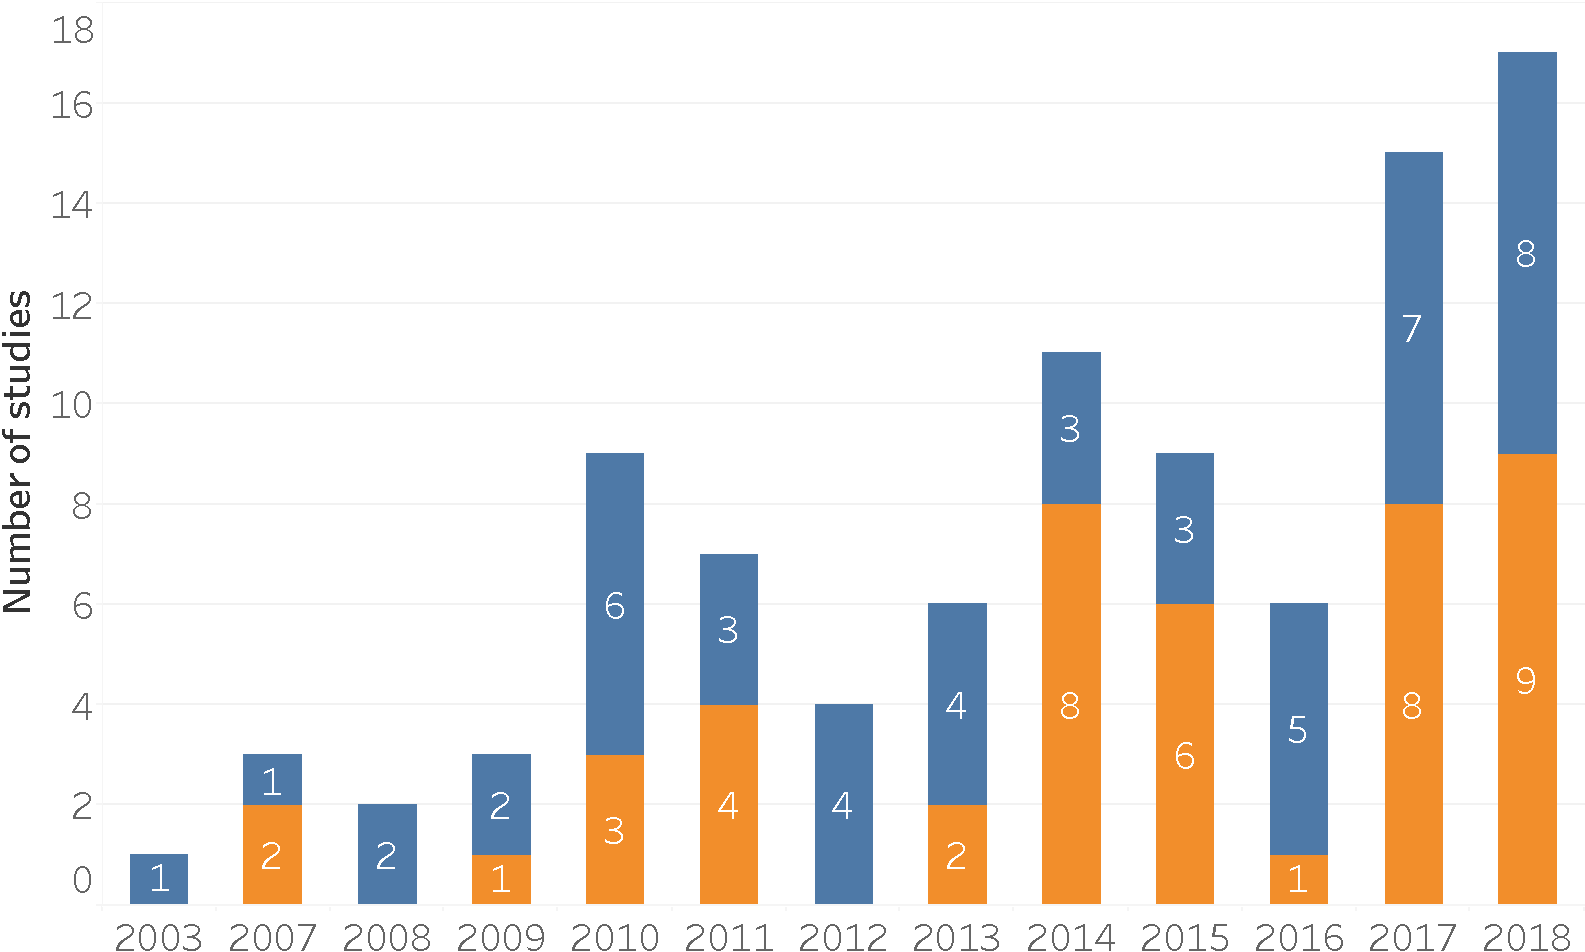
\includegraphics[width=\textwidth]{study_per_year}
\caption[Studies per year of publication]{This stacked barplot represents the number of included studies per year of publication. Blue studies have been presented in a conference, while orange studies have been published in a journal.}
\label{mcr:fig:study-per-year}
\end{figure}

\begin{figure}
\centering
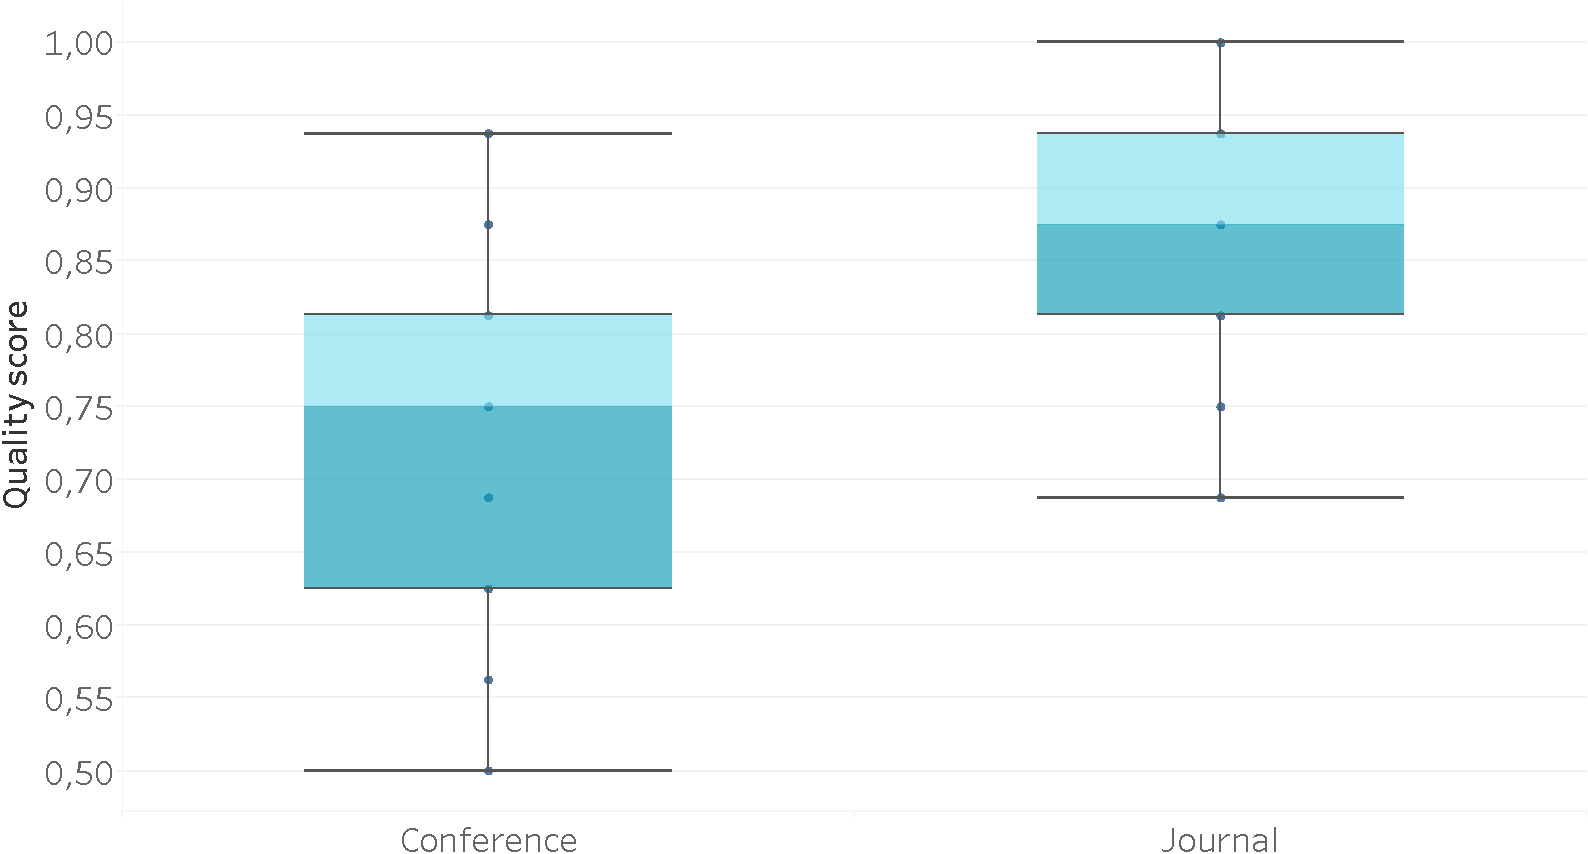
\includegraphics[width=\textwidth]{quality_per_type}
\caption[Quality scores per publication type]{This boxplot represents the distribution of quality scores per publication type. Studies published in journals have higher quality scores.}
\label{mcr:fig:quality-per-type}
\end{figure}

\begin{figure}
\centering
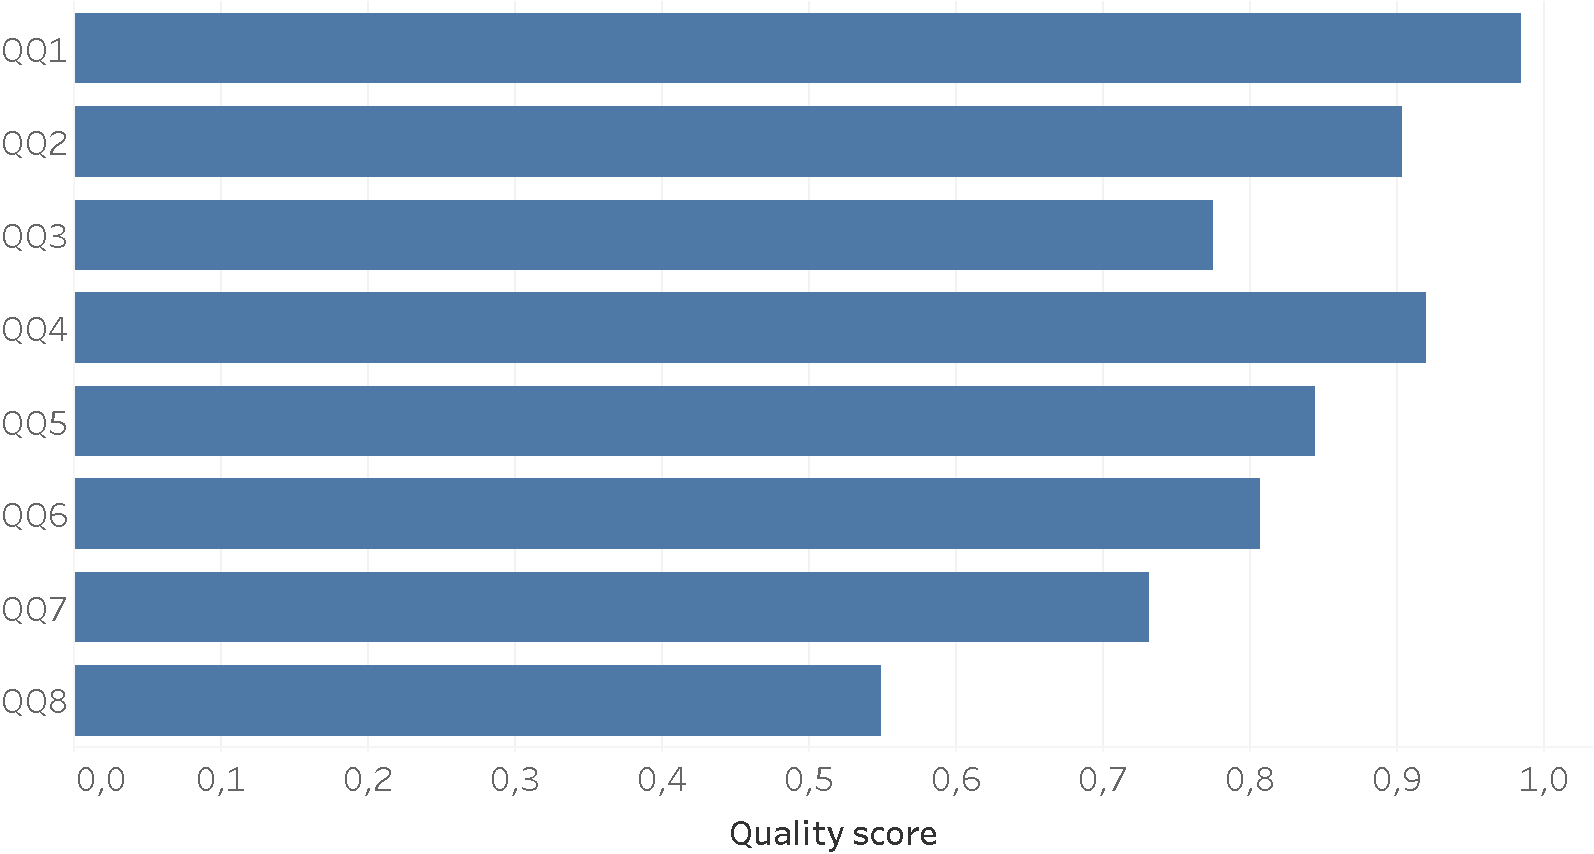
\includegraphics[width=\textwidth]{quality_per_question}
\caption[Quality score per quality question]{This barplot represents the average quality score per quality question. The lowest quality score is associated with the description of future works.}
\label{mcr:fig:quality-per-question}
\end{figure}

\subsection{Research Problems}
\label{mcr:sec:problems}

In this section, we describe the main problems and challenges that multicriteria recommender systems aim to address and, thus, we provide an answer to \ref{mcr:itm:rq2}. In total, we identified 10 different categories of problems that are mentioned in the reviewed studies. The number of studies for each category is summarized in Figure~\ref{mcr:fig:study-per-problem}. It is important to observe that a single study may \added{analyze} different problems at the same time.

\subsubsection{Data Sparsity}

Data sparsity is the most frequent problem in this field and it is caused by the fact that users provide ratings for a limited number of items or criteria. While this is a well documented common issue of recommender systems, multicriteria user-item matrices may be even sparser, as they require more effort and time from the users of the system. In order to address this problem, several solutions are proposed in the reviewed studies. For example, the authors of \pref{slr:Jannach2012} suggest to combine the multicriteria ratings using two different regression functions, one for the items and one for the users. The ratings estimated by the regression functions are then combined in order to minimize the prediction error. In \pref{slr:Samatthiyadikun2013}, a Bayesian latent model for multicriteria recommenders is exploited along with a support vector regression learner in order to mitigate the data sparsity problem. Another possible solution, as suggested in \pref{slr:Premchaiswadi2013}, is represented by dimensionality reduction techniques, which can be used to obtain a more compact representation of each user. Finally, it is possible to integrate the available ratings with an external ontology~\pref{slr:Liu2010} or with a trust-based model~\pref{slr:Goswami2017}. The data sparsity problem was identified in a total number of 22 studies.

\subsubsection{Criteria Weights}
\label{mcr:sec:criteria-weights}

In order to provide accurate suggestions, it is of paramount importance being able to discover the relationships among the different criteria and to identify the most relevant ones for the target user. A wide range of possible solutions is available in the analyzed studies. For instance, the authors of \pref{slr:Sreepada2017} identify the most important criteria for a user exploiting a statistical technique based on the average ratings of each item. Other studies analyze several machine learning methods. In \pref{slr:Zheng2017}, the author proposes to consider \emph{chains} of criteria instead of exploiting all criteria together: the rating on each criterion is estimated considering the previous predictions as context information. In \pref{slr:Choudhary2017}, the optimal weights are learned using particle swarm optimization, while in \pref{slr:Ding2018b} an artificial neural network is exploited for this purpose. Another popular solution is represented by decision making methods. As an example, in \pref{slr:Song2018} users are asked to perform pair-wise comparisons of the available criteria. The problem of selecting proper criteria weights was explicitly mentioned in 17 studies.

\subsubsection{\added{Personalization}}
\label{mcr:sec:personalization}

Any recommender system should be capable of suggesting items that match the preferences of the target user. The possibility of exploiting multiple ratings for each item is often considered an effective way of increasing the accuracy of the recommendations, for example this fact is mentioned in \pref{slr:Shambour2010} and \pref{slr:Mikeli2015}. It is also important being able to understand what are the most relevant criteria for each user, as suggested by the authors of \pref{slr:Sreepada2017}. On the other hand, it is essential to avoid including criteria that are redundant, as this may negatively affect the performance of the system~\pref{slr:Yin2009}. In \pref{slr:Castillo2018}, a multicriteria recommender system is combined with a content-based approach in order to generate better suggestions, while the authors of \pref{slr:Tallapally2018} propose to increase the accuracy of the recommendations using a deep learning technique called Stacked Autoencoders. In general, this problem was explicitly considered by 15 studies.

\subsubsection{Data Noise}
\label{mcr:sec:data-noise}

The presence of noise in data is typically related to the fact that users may provide ratings that are biased or even dishonest. For example, users may not understand the meaning of each criterion \added{and} may find difficult to express their preferences on a numerical scale, or may be bored by the request of assigning many ratings to a single item. In \pref{slr:Kant2017}, fuzzy logic techniques are exploited in order to \added{address} the uncertainty of user preferences, while in \pref{slr:Goswami2017} such techniques are combined with a trust-based model. The authors of \pref{slr:Jannach2012} propose to mitigate this problem by performing feature selection in a pre-processing step, where the most relevant criteria of a certain dataset are identified. Another possible solution to this problem is represented by the idea of considering the numerical differences between ratings instead of their absolute values in the recommendation process~\pref{slr:Mikeli2015}. Data noise was addressed by 14 studies.

\subsubsection{Cold-start}
\label{mcr:sec:cold-start}

The cold-start problem is a well-known issue in the field of recommender systems based on collaborative filtering approaches. It can be defined as the impossibility of creating reliable suggestions due to the lack of data regarding a new user or a new item. The authors of \pref{slr:Palanivel2011} aim to solve it by providing non-personalized recommendations to new users and exploiting content-based features when a new item is added to the system. A different approach is represented by the elicitation of user preferences using decision making techniques and multicriteria ratings \pref{slr:Hdioud2014}. In \pref{slr:Akcayol2018}, a multicriteria implicit feedback method based on user behavior analysis is discussed, while the authors of \pref{slr:Shambour2010} propose to tackle this issue with a trust-based model. As a last example, a knowledge-based method that is immune to the cold-start problem is illustrated in \pref{slr:Niknafs2008}. Cold-start was considered a research issue in 14 studies.  

\subsubsection{Scalability}
\label{mcr:sec:scalability}

Scalability is a general problem of collaborative filtering recommender systems, especially \added{for} the ones developed in an academic context \added{as proof-of-concept}. Because many multicriteria recommenders require multiple runs of such algorithms, it is reasonable to suppose that scalability issues are even more widespread. For example, this issue is discussed by the authors of \pref{slr:Wijayanto2016}, who describe a multicriteria recommender that exploits a distributed architecture based on Apache Spark. In \pref{slr:Mikeli2015}, a clustering algorithm is applied for creating groups of similar users that can be used to compute predictions in a scalable way. A popular dimensionality reduction technique discussed by \pref{slr:Bokde2015} and \pref{slr:Nilashi2014b} is the higher order single value decomposition. In total, 12 studies considered the scalability problem.

\subsubsection{User's Effort}

As multicriteria recommenders usually require many ratings for each user and item pair, explicit elicitation methods are intrusive and may waste the user's effort and time. For this reason, the authors of \pref{slr:Palanivel2010} and of \pref{slr:Nunez-Valdez2018} propose a multicriteria recommender based only on implicit feedback. Another possible solution is described in \pref{slr:Premchaiswadi2013}, where \added{their} authors develop a hybrid profiling framework for reusing traditional ratings with multicriteria recommenders. A similar approach to this problem is presented in \pref{slr:Castillo2018}, where multicriteria ratings are computed starting from single ratings and content-based information. This problem was discussed by 11 studies.

\subsubsection{Other Research Problems}

Other research problems are mentioned in a more limited number of studies. In particular, 4 studies analyzed the issues related to the selection of a proper similarity metric in the context of multidimensional neighborhood-based collaborative filtering, while 3 studies reported the challenges related to the execution of a reliable evaluation protocol. Finally, 3 more recent studies mentioned the problem of fairness in the selection of the recommended items, both with respect to the unique peculiarities of the users and to the characteristics of the catalog.

\begin{figure}
\centering
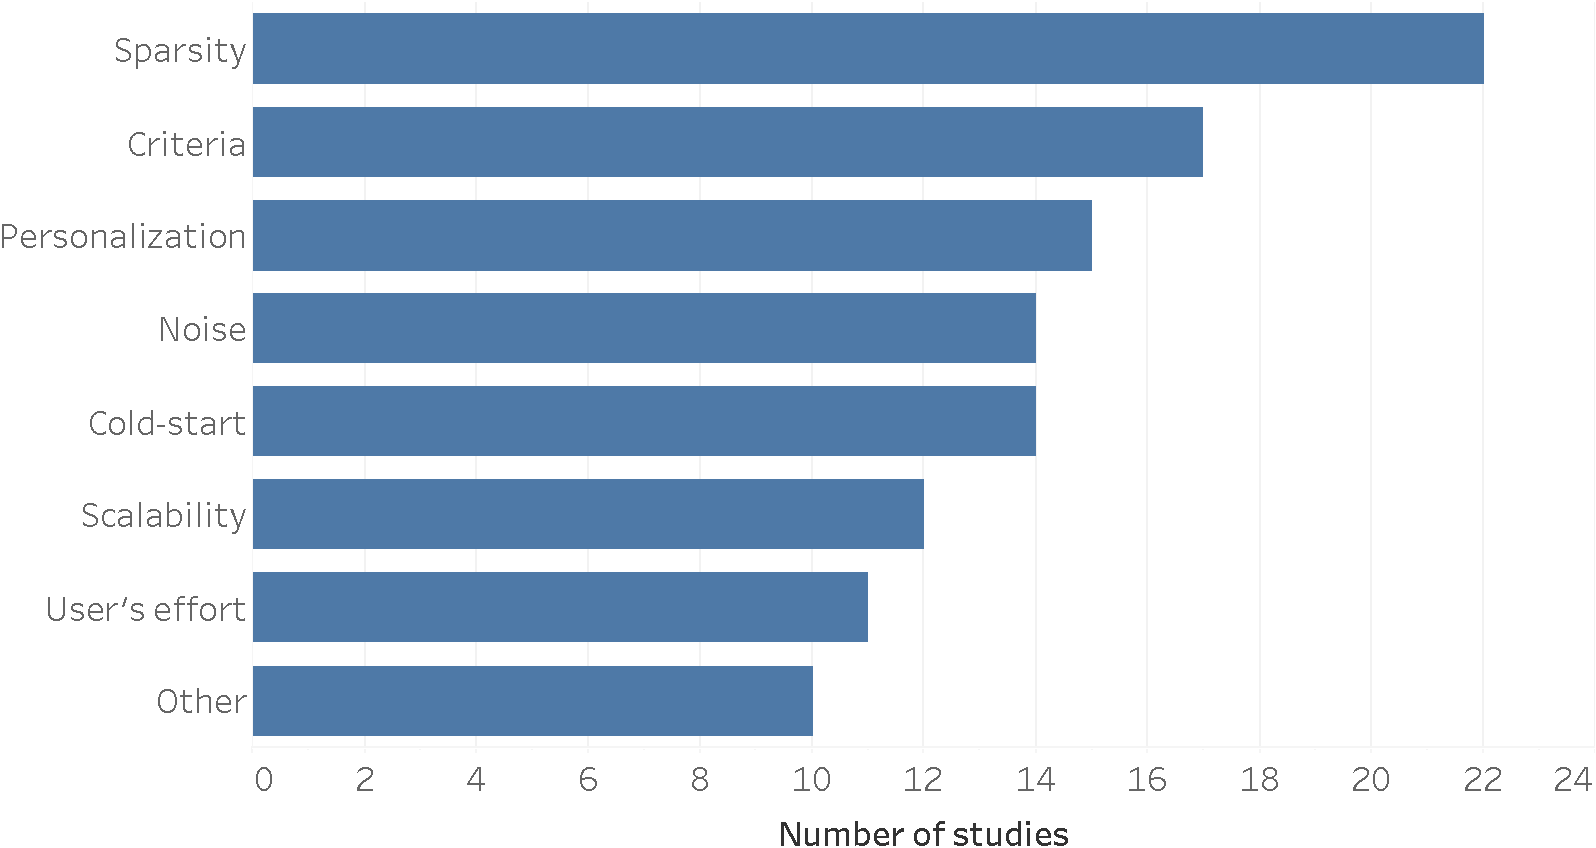
\includegraphics[width=\textwidth]{problem_per_study}
\caption[Studies per research problem]{This barplot represents the number of studies per research problem.}
\label{mcr:fig:study-per-problem}
\end{figure}

\subsection{Recommendation Approaches}
\label{mcr:sec:approaches}

In order to provide an answer to \ref{mcr:itm:rq3}, we analyzed the studies included in this systematic literature review and we classified them according to the taxonomy provided by Burke~\cite{Burke2007}. This taxonomy has become a widespread way of characterizing different recommendation approaches. However, we decided not to consider hybrid recommender systems, as almost all multicriteria recommenders would fall in this category. For this reason, if a study combines multiple approaches, it will be included in all the categories of the different methods that are mentioned in the study. We summarize the number of available studies for each recommendation approach in Table~\ref{mcr:tab:study-per-approach}.

\subsubsection{Collaborative Filtering}

Collaborative filtering is the most popular recommendation technique described in the reviewed literature. In a traditional recommender system, the users whose rating behaviour is similar to the one of the target user are exploited for selecting the items to be suggested. In a multicriteria recommender, a popular approach consists in applying collaborative filtering algorithms on the available criteria and then combining the results in a global estimated rating, like in \pref{slr:Hwang2010} and \pref{slr:Manouselis2007}. An alternative to the user-based approach is represented by the item-based collaborative filtering, where the similarity is computed among the items, as discussed, for example, in \pref{slr:Bilge2014}. \added{The authors of} \pref{slr:Jannach2012} and \pref{slr:Kermany2017} describe how to combine user-based and item-based models in a comprehensive approach. Collaborative filtering may also be implemented with a model-based approach, for instance matrix factorization (e.g., in \pref{slr:Asawarangsee2016} and \pref{slr:Majumder2017}). In general, this technique may be combined with other methods, like content-based approaches~\pref{slr:Zarrinkalam2012}, clustering~\pref{slr:Mikeli2015}, and fuzzy logic~\pref{slr:Palanivel2011}. In total, collaborative filtering was exploited by 82 studies.

\subsubsection{Content-based}

A content-based recommender system considers the previous preferences of a user in order to build a profile and to select items with similar characteristics. For example, the authors of \pref{slr:Naak2009} describe a recommender system of research papers that relies on content-based and multicriteria collaborative filtering algorithms. In \pref{slr:Amoretti2017}, user profiles are created from multicriteria ratings and, then, they are exploited for building clusters of similar users. The authors of \pref{slr:Palanivel2010} suggest to identify the user's category-wise preferences for each criterion with a content-based approach. A possible source of structured information regarding items are external ontologies, \added{as they are} discussed in \pref{slr:Zarrinkalam2012}. In \pref{slr:Musto2017} and \pref{slr:Sharma2015}, user's reviews are mined to identify the most important features of each item. Content-based approaches were mentioned by 16 studies.

\subsubsection{Knowledge-based}

A knowledge-based recommender system relies on an externally encoded domain knowledge in order to match the user profiles with certain item features. For example, in \pref{slr:Pinandito2015} a mobile recommender suggests restaurants considering their geographical location and cuisine. The author of \pref{slr:Yuen2017} describes a method for asking \added{users} to express \added{their} preferences regarding the features of a smartphone. In a similar vein, the recommender system presented in \pref{slr:Karacapilidis2003} exploits user profiles and fuzzy set theory in order to suggest cities to be visited. In \pref{slr:Akcayol2018}, the authors of the study propose a set of rules for building a personalized list of recommended movies. Knowledge-based techniques were identified in 12 studies.

\subsubsection{Community-based}

If a recommender system also considers the relations of friendship and trust among its users, it is defined as community-based. For example, the authors of \pref{slr:Goswami2017} propose a multicriteria collaborative filtering recommender that is enhanced by considering trust as an additional weight during the hybrid prediction phase. A similar approach is followed by \pref{slr:Shambour2011b} and \pref{slr:Leal2017b}, where the trust score for each user is computed only considering rating data and it is combined with the results of a collaborative filtering algorithm. Community-based recommenders were discussed by 5 studies.

\subsubsection{Demographic}

A demographic recommender considers the demographic profile of the user for suggesting items. For example, the authors of \pref{slr:Dixit2014} describe a multicriteria recommender for groups where users are clustered also according to their demographic profile. The other studies that mention demographic information are \pref{slr:Kermany2017}, \pref{slr:Amoretti2017}, and \pref{slr:Zheng2018}. Demographic recommenders were considered by 4 studies.

\begin{table}
\centering
\begin{tabular}{@{}ll@{}}
\toprule
Approach                & Studies \\ \midrule
Collaborative filtering & 82      \\
Content-based           & 16      \\
Knowledge-based         & 12      \\
Community-based         & 5       \\
Demographic             & 4       \\ \bottomrule
\end{tabular}
\caption[Studies per recommendation approach]{The number of studies per recommendation approach.}
\label{mcr:tab:study-per-approach}
\end{table}

\subsection{Multicriteria Techniques}
\label{mcr:sec:techniques}

In the following, we analyze the main techniques and methods related to multicriteria recommender systems that we identified in the reviewed studies and, therefore, we provide an answer to \ref{mcr:itm:rq4}. In most studies, the recommenders combine different techniques, for example \textit{k}-NN may be exploited to estimate unknown ratings, while decision analysis to merge the different ratings in a global prediction. We summarize the most frequent ones in Table~\ref{mcr:tab:study-per-technique}.

\subsubsection{\textit{k}-NN}

\textit{k}-NN is a classification method used in data mining applications that relies on the similarity of the instances to be classified with the training examples. In the context of collaborative filtering, \textit{k}-NN is exploited to find similar users or items considering their neighborhood. For example, in \pref{slr:Hwang2010}, a \textit{k}-NN collaborative filtering method is applied to each criterion separately, like in traditional recommenders. In contrast, a different approach to this problem is considering all the criteria together when applying the \textit{k}-NN algorithm. To this end, it is necessary to rely on a multidimensional distance, like the Manhattan, Euclidean, or Chebyshev distance, as described in \pref{slr:Adomavicius2007}. \textit{k}-NN is the most popular \added{data mining technique applied to multicriteria recommender systems}, as it was identified in 35 studies.

\subsubsection{Decision Analysis}

In order to rank items with contrasting criteria, it is possible to exploit the tools provided by multiple-criteria decision analysis, which is a sub-field of operations research. In general, different methods are available in order to support users in making complex decisions, and some of these methods have also been applied to multicriteria recommender systems. For example, in \pref{slr:Li2014}, an analysis hierarchy process (AHP) is used in order to help users to evaluate the relative importance of each criterion. In \pref{slr:Lakiotaki2011}, the UTA* algorithm is exploited for constructing user profiles that are subsequently grouped according to their preferences. Other decision analysis methods mentioned in the reviewed studies are, for instance, ELECTRE~\pref{slr:Hu2014}, SMART~\pref{slr:Huang2011}, TOPSIS~\pref{slr:Dixit2014}, and UTADIS~\pref{slr:Matsatsinis2009}. In total, decision analysis techniques were identified in 26 studies.

\subsubsection{Fuzzy Logic}

Fuzzy logic is a mathematical model that can be used to represent the concept of partial truth. This model is exploited to formalize the vagueness and uncertainty that are usually associated with user ratings. For example, in \pref{slr:Boulkrinat2013}, \pref{slr:Palanivel2011}, and \pref{slr:Hamada2018}, ratings are expressed using linguistic terms in a qualitative way, considering that each term may have a different meaning according to the user. Furthermore, the authors of \pref{slr:Pinandito2015} use the AHP decision analysis method in the fuzzy domain using fuzzy numbers instead of real numbers. In \pref{slr:Nilashi2014b}, fuzzy rules that express how to build global ratings are identified for each cluster of users. Fuzzy logic was exploited as a recommendation technique in 16 studies.

\subsubsection{Regression Analysis}

Regression analysis is a set of statistical techniques for predicting the value of a dependent variable given one or more independent variables. In the reviewed studies, such techniques are typically used to estimate the global rating of an item considering the predicted ratings for each criterion. For example, the authors of \pref{slr:Majumder2017} find the weights of the aggregation function with a linear regression model that is learned for each user. In \pref{slr:Jhalani2016}, a non-personalized linear regression model is first used to aggregate the similarities among users, and then to estimate the final ratings. A different approach is represented by Support Vector Regression (SVR): for instance, in \pref{slr:Fan2013}, a SVR model is trained for each user in order to synthesize the overall rating. We found regression analysis techniques in 15 studies.

\subsubsection{Clustering}

Clustering is an exploratory data mining approach that consists in grouping objects in cohesive sets. A typical application of such techniques to multicriteria recommender systems is represented by the identification of users with similar profiles. For instance, in \pref{slr:Mikeli2015}, \pref{slr:Lakiotaki2011}, and \pref{slr:Wasid2018}, the global K-means clustering algorithm is exploited in order to create groups of users with similar preferences. In \pref{slr:Fan2013}, clusters of users are created according to the importance given to each criterion. On the other hand, the authors of \pref{slr:Lousame2010} propose to cluster the items and, then, to learn an aggregation function for each user and item cluster. A clustering technique is also exploited to identify malicious users in the context of robust recommenders~\pref{slr:Turk2018}. In total, clustering algorithms were mentioned in 15 studies.

\subsubsection{Matrix Manipulation}

In the reviewed studies, we identified different techniques used to compute predicted ratings with mathematical operations on matrices. For example, in \pref{slr:Ko2017}, the Singular Value Decomposition (SVD) method is exploited to compute unknown ratings for each criterion. In contrast, the authors of \pref{slr:Bokde2015} propose to reduce the dimensionality of the user, item, and criterion tensor with the Higher-Order Singular Value Decomposition (HOSVD) method and then to apply a collaborative filtering algorithm to the resulting matrix. In \pref{slr:Agathokleous2014}, a matrix factorization technique is applied to a utility matrix estimated from the multicriteria ratings using a neural network model trained considering each user. A different approach is followed by the authors of \pref{slr:Ding2018}, which proposes a factorization machine model for representing all multicriteria ratings together. Matrix manipulation techniques were discussed in 12 studies.

\subsubsection{Neural Networks}

Neural networks are usually applied to multicriteria recommender systems in order to aggregate the predicted ratings for each criterion in a global score. For example, in \pref{slr:Wijayanto2016}, a single layer PERCEPTRON algorithm is selected for this task, while the authors of \pref{slr:Hassan2017} propose a neural network trained with the simulated annealing algorithm. In \pref{slr:Nilashi2014b}, an Adaptive Neuro-Fuzzy Inference System (ANFIS) is exploited for extracting fuzzy rules for each cluster of users; such rules are later applied to predict the overall rating. A different approach is described in \pref{slr:Ding2018b}, where a neural factorization machine is used to model the interactions among users, items, and criteria, and in \pref{slr:Hu2014}, where a single layer PERCEPTRON is exploited to estimate the similarity among users. We identified neural network approaches in 12 studies.

\subsubsection{Genetic Algorithms}

Genetic algorithms can be considered a family of optimization techniques and, in the reviewed studies, they are typically used to determine the weights of each criterion. For example, in \pref{slr:Hwang2010b} and \pref{slr:Parveen2015}, a genetic algorithm is run for each user in order to construct a personalized aggregation function. In contrast, the authors of \pref{slr:Jannach2012} propose to use it for performing a feature selection of the available criteria in order to identify an optimal set of dimensions. In total, genetic algorithms were exploited by 7 studies.

\subsubsection{Other Techniques}

Other less frequent techniques described in the reviewed studies include statistical modeling~\pref{slr:Samatthiyadikun2013}, particle swarm optimization~\pref{slr:Choudhary2017}, and natural language processing~\pref{slr:Liu2013}. Such techniques were found in 7 studies.

\begin{table}
\centering
\begin{tabular}{@{}ll@{}}
\toprule
Technique           & Studies \\ \midrule
\textit{k}-NN                & 35      \\
Decision analysis   & 26      \\
Fuzzy logic         & 16      \\
Regression analysis & 15      \\
Clustering          & 15      \\
Matrix manipulation & 12      \\
Neural networks     & 12      \\
Genetic algorithms  & 7       \\
Other               & 7       \\ \bottomrule
\end{tabular}
\caption[Studies per recommendation technique]{The number of studies per recommendation technique.}
\label{mcr:tab:study-per-technique}
\end{table}

\subsection{Application Domains}
\label{mcr:sec:domains}

We analyzed the application domains of the multicriteria recommender systems described in the reviewed studies in order to provide an answer to \ref{mcr:itm:rq5}. A graphical summary listing the categories of recommended items, considering possible examples and the experimental evaluation, is available in Figure~\ref{mcr:fig:domain-per-study}. We observe that the majority of studies propose to apply multicriteria recommenders to domains related to tourism and travel. For example, 13 studies describe recommenders for hotels, 9 related to restaurants, and 4 dealing with tourist places. Another popular domain is related to movies, mentioned in 8 studies. Other domains include consumer electronics products and education, described in 7 and 5 studies respectively. Research papers were discussed in 3 studies, while medical treatments and music in 2 studies each. Less popular domains, identified only in 1 study and grouped in a miscellaneous category, are business and romantic partners, investment solutions, electronic books, and job opportunities.
	
\added{Different categories of criteria are selected by researchers according to the domain. For example, popular criteria for hotels are \textit{rooms}, \textit{location}, \textit{cleanliness}, \textit{service}; for restaurants \textit{food quality}, \textit{service}, \textit{presentation}, \textit{taste}; for tourist places \textit{architectural style}, \textit{ease of access} and \textit{welcome quality}; for movies \textit{story}, \textit{acting}, \textit{direction} and \textit{visuals}; for consumer electronics products \textit{type}, \textit{brand}, \textit{weight}, \textit{size}; for learning resources \textit{subject relevance} and \textit{educational value}.}

\begin{figure}
\centering
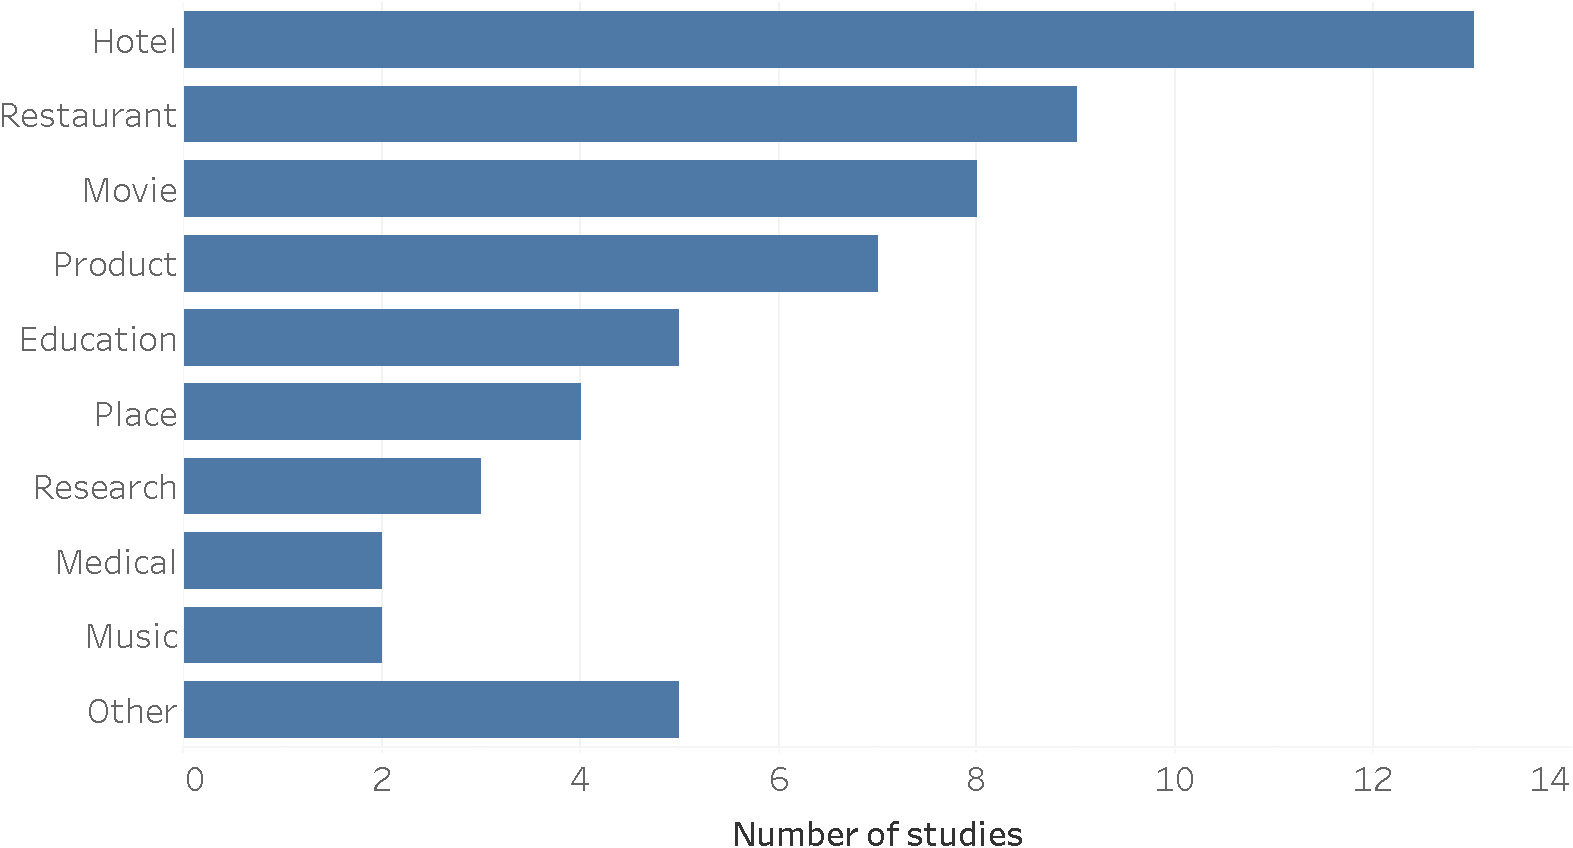
\includegraphics[width=\textwidth]{domain_per_study}
\caption[Studies per application domain]{This barplot represents the number of studies per application domain.}
\label{mcr:fig:domain-per-study}
\end{figure}

\subsection{Evaluation Protocols}
\label{mcr:sec:protocols}

In this section, we describe the evaluation protocols followed by the reviewed studies, in line with \ref{mcr:itm:rq6}. We grouped the possible evaluation strategies in four main categories, which are summarized in Table~\ref{mcr:tab:protocols}.

\subsubsection{Offline Comparison}

We discovered that 74 studies compare the proposed solution with other approaches using an offline evaluation. Multicriteria recommender systems are usually compared \added{against} traditional baselines such as single-criteria recommender or weighted average multicriteria approaches. Different studies consider the most similar methods already available in literature, while few studies only compare the described technique with itself, analyzing several configuration parameters.

\subsubsection{User Study}

A different approach is represented by the execution of user studies, which were carried out in 12 works. For example, the authors of \pref{slr:Akcayol2018} created a movie recommender system that was tested by 567 users. The researchers computed different metrics considering their behaviour while utilizing the recommender. In contrast, in \pref{slr:Li2015} 158 users were asked to fill out a questionnaire in order to compare different recommendation models. User studies are also exploited to evaluate the usability of the system, as done, for instance, in \pref{slr:Akhtarzada2011}.

\subsubsection{Case Study}

We also identified 4 studies that evaluated the proposed approach by describing a case study. For example, in \pref{slr:Hdioud2013}, a possible application of a multicriteria recommender to the movie domain is discussed, while the authors of \pref{slr:Lee2007} empirically compare the suggested restaurants considering different user profiles.

\subsubsection{No Evaluation}

Finally, 3 studies performed no evaluation of the multicriteria recommender presented in the paper. For example, in \pref{slr:Shambour2010}, the evaluation of the proposed model is left as a future work.

\begin{table}
\centering
\begin{tabular}{@{}ll@{}}
\toprule
Evaluation protocol & Studies \\ \midrule
Offline comparison  & 74      \\
User study          & 12      \\
Case study          & 4       \\
No evaluation       & 3       \\ \bottomrule
\end{tabular}
\caption[Studies per evaluation protocol]{The number of studies for each evaluation protocol.}
\label{mcr:tab:protocols}
\end{table}

\subsection{Evaluation Metrics}
\label{mcr:sec:metrics}

In the following, we discuss the metrics exploited in the reviewed studies for conducting the experimental evaluation of the proposed solutions in order to answer to \ref{mcr:itm:rq7}. We decided to classify them according to the dimensions related to the recommender system proprieties described by Gunawardana et al.~\cite{Gunawardana2015}. The identified category for each evaluation metric and the associated number of studies are reported in Table~\ref{mcr:tab:metrics}.

\subsubsection{Rating Accuracy}

This category includes metrics designed to evaluate the capability of the system to correctly estimate user ratings. In particular, 51 studies report the Mean Absolute Error (MAE), 20 the Root Mean Squared Error (RMSE), and 3 the Mean Squared Error (MSE). Other metrics exploited by 1 study each are the coefficient of determination ($R^2$) and the Mean Absolute Percentage Error (MAPE). In total, rating accuracy metrics are mentioned in 59 studies.

\subsubsection{Usage Accuracy}

If the goal of a recommender is to predict a list of items, it is possible to evaluate the usage accuracy of the available suggestions. Precision is considered in 36 studies, recall in 28, F1 in 23 studies, and Area Under the Curve (AUC) in 4 studies. Usage accuracy is the second most popular category, as it was identified in 43 studies.

\subsubsection{Coverage}

The metric of coverage was computed in 11 studies. Even if this metric can be evaluated both at the level of users and at the level of items, all the studies included in this review considered the coverage of the item space, also known as catalog coverage~\cite{Herlocker2004}.

\subsubsection{Ranking Accuracy}

The correctness of the ranking in the recommended lists of items was analyzed by 10 studies. In details, 8 studies exploit the Normalized Discounted Cumulative Gain (nDCG) metric, while 4 studies the Fraction of Concordant Pairs (FCP). A less popular metric, described by 1 study, is the Kendall's $\tau$.

\subsubsection{Scalability}

The authors of 8 studies evaluated the scalability of the proposed approach. A typical metric used to this purpose is the time required to compute the predictions, which is reported by 6 studies. In contrast, 2 studies exploit the speed of the recommendations.

\subsubsection{Other Metrics}

Additional metrics identified in the reviewed studies include the utility of the suggested items and the system satisfaction, evaluated with a user study, and the robustness of the recommendations. Finally, the authors of \pref{slr:Manouselis2014} defined a combined metric.

\begin{table}
\centering
\begin{tabular}{@{}ll@{}}
\toprule
Evaluation metric & Studies \\ \midrule
Rating accuracy   & 59      \\
Usage accuracy    & 43      \\
Coverage          & 11      \\
Ranking accuracy  & 10      \\
Scalability       & 8       \\
Other             & 5       \\ \bottomrule
\end{tabular}
\caption[Studies per evaluation metric]{The number of studies for each evaluation metric.}
\label{mcr:tab:metrics}
\end{table}

\subsection{Evaluation Datasets}
\label{mcr:sec:datasets}

In line with \ref{mcr:itm:rq8}, we analyzed the datasets exploited for conducting the experimental evaluation of the techniques described in the reviewed studies. In total, 74 studies mentioned at least one dataset: this result is consistent with the number of studies that performed an offline comparison, as reported in Section~\ref{mcr:sec:protocols}. We summarize the studies for each dataset in Figure~\ref{mcr:fig:dataset-per-study}.

\subsubsection{Yahoo! Movies}

Yahoo! Movies was a website, part of the Yahoo! network, that provided information and reviews about movies. Among other features, users were able to rate each movie considering five criteria: story, acting, direction, visuals, and overall. Yahoo! Research provides a public Yahoo! Movies dataset, but it does not include multicriteria ratings.\footnote{\url{https://webscope.sandbox.yahoo.com}} To address this issue, the authors of \pref{slr:Jannach2012} created a multicriteria version of the same dataset by crawling the Yahoo! Movies website. In total, 36 studies exploit the Yahoo! Movies dataset, either the version obtained by Jannach et al.~\pref{slr:Jannach2012} or other versions crawled by different researchers, \added{such as \pref{slr:Samatthiyadikun2013}, \pref{slr:Yin2009}, and \pref{slr:Adomavicius2007}.}

\subsubsection{TripAdvisor}

TripAdvisor is a website that contains restaurant and hotel reviews. Similarly to Yahoo! Movies, there is no official multicriteria rating dataset, as different researchers crawled the website and created their own version, typically exploiting hotel ratings and reviews. For example, this approach was followed by the authors of \pref{slr:Liu2010} and \pref{slr:Jannach2014}. The TripAdvisor dataset collected by the authors of \pref{slr:Liu2011} is publicly available.\footnote{\url{https://www.cs.cmu.edu/~jiweil/html/hotel-review.html}} Also the TripAdvisor dataset created by Wang et al.~\cite{Wang2010} and used in \pref{slr:Leal2017b} is available online.\footnote{\url{http://www.cs.virginia.edu/~hw5x/Data/LARA/TripAdvisor}} In total, the TripAdvisor dataset was mentioned by 19 studies.

\subsubsection{In-house}

We identified 9 studies that created a multicriteria dataset in-house for conducting an offline comparison. For example, the authors of \pref{slr:Palanivel2011} collected 9,628 ratings about songs that were later used to evaluate a music recommender system. In \pref{slr:Bokde2015}, different students were invited to provide ratings about universities.

\subsubsection{MovieLens}

Even if the MovieLens datasets only contain single criteria ratings, they were also exploited for evaluating multicriteria recommender systems. For instance, in \pref{slr:Shambour2011} \added{and in \pref{slr:Shambour2011b}}, MovieLens~100K was transformed in a four criteria dataset. A similar approach was followed in \pref{slr:Castillo2018} with MovieLens~10M, where a method capable of extracting multicriteria preferences from traditional ratings \added{using external aggregate ratings and descriptive data} is discussed. In total, the MovieLens datasets were mentioned by 5 studies.

\subsubsection{Synthetic}

Because of the lack of public multicriteria datasets, some researchers created synthetic ratings in order to evaluate their approach. For example, the authors of \pref{slr:Matsatsinis2009} simulated a dataset about equity fund recommendations. In \pref{slr:Manouselis2008}, a testing tool named CollaFiS, capable of building multicriteria datasets, is discussed. This approach was followed by 4 studies.

\subsubsection{Other Datasets}

Less common datasets, exploited by 1 or 2 studies each, include, for example, Bcn Restaurantes~\pref{slr:Marin2014}, HRS.com~\pref{slr:Leal2017b}, and RateBeer~\pref{slr:Ding2018b}. Such various datasets were considered by 18 studies.

\begin{figure}
\centering
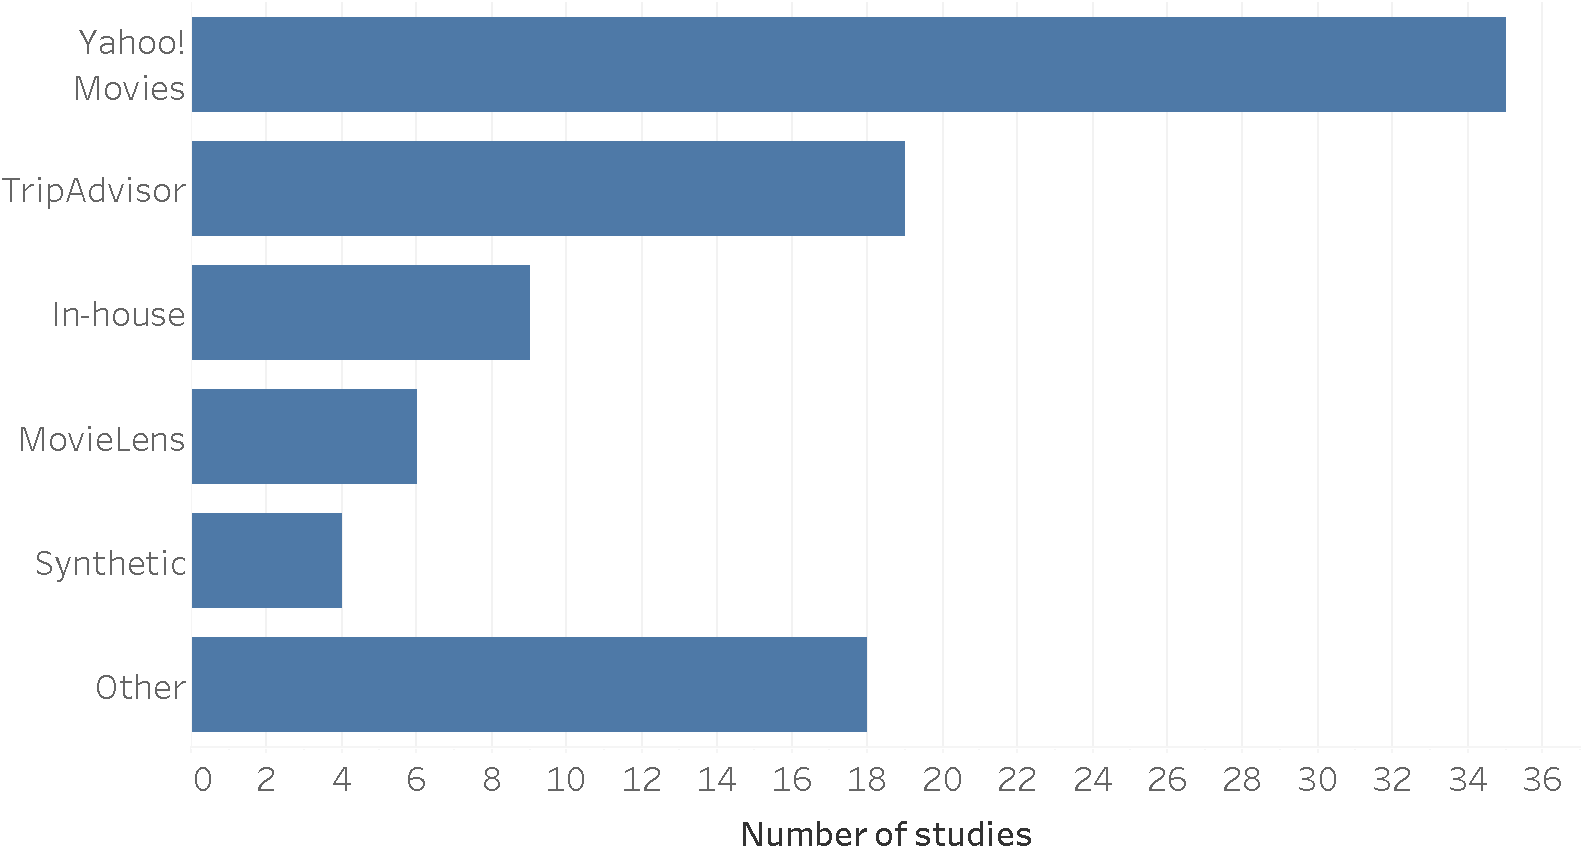
\includegraphics[width=\textwidth]{dataset_per_study}
\caption[Studies per evaluation dataset]{This barplot represents the number of studies per evaluation dataset.}
\label{mcr:fig:dataset-per-study}
\end{figure}

\subsection{Future Works}
\label{mcr:sec:future}

In the following, we analyze the suggestions for future works mentioned in the reviewed studies in order to provide an answer to \ref{mcr:itm:rq9}. A summary of our findings is available in Table~\ref{mcr:tab:future}.

\subsubsection{Extend the Solution}

Different authors propose to extend or modify the described recommender system for increasing its accuracy. \added{This future work is related to the problem of personalization, discussed in Section~\ref{mcr:sec:personalization}.} Common suggestions include adding additional components like clustering algorithms or further recommendation models and exploiting soft-computing techniques. In total, we identified this \added{future work} in 33 studies.

\subsubsection{Include More Data or Additional Criteria}

Another possibility is to improve the proposed approach by including more data or by increasing the number of criteria exploited by the recommendation algorithm. For example, it is possible to rely on external ontologies, contextual and content information, trust-related scores, and also consider additional criteria extracted from user reviews. This category of future works was mentioned in 24 studies.

\subsubsection{Improve the Evaluation}

Some studies mention the fact that the evaluation performed by their authors was not enough complete or detailed because of different kinds of constrains. For this reason, it would be advisable to increase its trustfulness by executing it again considering more datasets, techniques, and evaluation metrics. In total, this problem was reported by 14 studies.

\subsubsection{Identify Significant Criteria}

A common issue associated with multicriteria recommenders is the noise introduced by redundant criteria, \added{as discussed in Section~\ref{mcr:sec:data-noise}}. For this reason, some authors considered the identification of the most significant criteria as a future work. This suggestion was discussed in 13 studies.

\subsubsection{Increase the Scalability}

A typical issue of multicriteria recommender systems is their limited scalability. \added{This problem was highlighted by different studies in Section~\ref{mcr:sec:scalability}.} Some researchers suggested to study how to increase it, for example by means of parallel computational paradigms. We identified this future work in 10 studies.

\subsubsection{Consider Different Domains}

Finally, 7 studies mentioned the necessity of validating the proposed approach in different domains, like it is usually done with traditional recommenders. However, this objective is difficult to achieve because of the limited availability of multicriteria \added{rating} datasets.

\subsubsection{Other Future Works}

Further categories of future works, mentioned in less than 5 studies each, include designing solutions for addressing the cold-start problem, \added{as described in Section~\ref{mcr:sec:cold-start},} performing experiments with adaptive recommenders, solving the issues related to preference elicitation, creating algorithms for explaining the recommendations, and performing an analysis of the related ethical problems.

\begin{table}
\centering
\begin{tabular}{@{}ll@{}}
\toprule
Future work                   & Studies \\ \midrule
Extend the solution           & 33      \\
Include more data or criteria & 24      \\
Improve the evaluation        & 14      \\
Identify significant criteria & 13      \\
Increase the scalability      & 10      \\
Consider different domains    & 7       \\
Other                         & 9       \\ \bottomrule
\end{tabular}
\caption[Studies per category of future work]{The number of studies per category of future work.}
\label{mcr:tab:future}
\end{table}

\section{Discussion}
\label{mcr:sec:discussion}

In the following, we discuss the outcome of our systematic literature review, considering the answers provided in Section~\ref{mcr:sec:results} to the research questions originally introduced in Section~\ref{mcr:sec:questions}, and highlighting possible threats to validity.

\subsection{Included Studies}

As reported in Figure~\ref{mcr:fig:study-per-year}, the \added{earliest} study included in this review, which is \pref{slr:Karacapilidis2003}, dates back to the year 2003. However, the field of multicriteria recommender systems started to be relatively widespread only from the year 2007, when influential studies like \pref{slr:Adomavicius2007} were published. We can also observe an increasing amount of publications, suggesting that this research topic is still popular, as recommender systems in general. \added{In particular, the last few years were characterized by a higher number of studies related to specialized applications of multicriteria approaches, for example in tourism, health and care, and distance learning.}

Regarding the quality of the included studies, summarized in Figure~\ref{mcr:fig:quality-per-type}, we can highlight the fact that higher scores were assigned to works published in journals with respect to conferences. This result is consistent with the conclusions of other systematic literature reviews conducted in related fields, like hybrid and linked data-based recommender systems \cite{Cano2017,Figueroa2015}.

\subsection{Research Problems}

By looking at the problems listed in Section~\ref{mcr:sec:problems}, it is possible to observe that the most frequent one faced by researchers is data sparsity. This is a general issue of collaborative filtering recommender systems that causes a lower recommendation quality due to an insufficient amount of input data. However, it is reasonable to suppose that data sparsity is more severe in the context of multicriteria recommenders, because of the higher amount of expected ratings. Possible solutions include the use of external information or the construction of latent models. In contrast, it is not clear what is the effect of using different rating elicitation methods.

Another typical research problem is discovering what are the optimal weights for each criterion. They may be computed globally or for each user with the objective of maximizing the recommendation accuracy. A second approach is to obtain the weights directly from the user, for example with decision making techniques.

A different but related issue is represented by data noise, caused by redundant criteria or dishonest ratings. Of course, in order to minimize the user's effort and the probability of obtaining inaccurate ratings, it is necessary to limit the number of criteria. However, identifying the most appropriate ones for a given domain is a difficult task even for an expert. In our opinion, this issue should be better investigated by future studies.

Accuracy is a characteristic required for any machine learning technique and, in the context of recommender systems, it is related to user satisfaction. Multicriteria recommenders can increase the \added{personalization} of the suggestions if they are capable of correctly identifying what are the most important criteria for each user. However, when a user is new to the system, the cold-start problem arises. This is a general issue of collaborative filtering recommenders and it is typically solved by creating hybrid solutions that consider content-based information.

Finally, the usage of multiple \added{criterion} results in algorithms that are less scalable. This problem can be addressed with clustering and dimensionality reduction techniques, as well as by exploiting distributed architectures.

\subsection{Recommendation Approaches}

The vast majority of multicriteria recommender systems can be classified as collaborative filtering approaches, as reported in Table~\ref{mcr:tab:study-per-approach}. For example, in heuristic-based methods, the ratings provided for each dimension are exploited together using a multidimensional distance metric, extending the traditional neighborhood-based recommendation technique. More complex heuristics rely on the aggregation of different similarities computed per criterion, possibly using weights specific for each user. Also in the context of model-based collaborative filtering, methods like matrix factorization are applied to each dimension and, then, their results are aggregated in a global predicted rating.

For this reason, almost all recommender systems included in this review can be considered hybrid, as they combine multiple collaborative filtering models, one for each criterion. Furthermore, such techniques are sometimes exploited together with content-based, knowledge-based, community-based, and demographic approaches, resulting in other forms of hybrid recommenders~\cite{Burke2007}.

However, a limited number of studies included in this review deals with recommender systems that can be classified only as knowledge-based. Such systems exploit domain specific knowledge to match the available items with the user preferences. They were selected because we identified them as a form of multicriteria recommendation, even if the distinction between knowledge-based recommenders and traditional information retrieval methods is not always clear.

\subsection{Multicriteria Techniques}

In Section~\ref{mcr:sec:techniques}, we reported that the most common technique exploited by multicriteria recommenders is the \textit{k}-NN algorithm. This result is consistent with the recommendation approaches identified in the reviewed studies, as neighborhood-based methods represent a popular approach of collaborative filtering. \textit{k}-NN may be enough to build a multicriteria recommender: the similarities among users or items can be directly computed with a multidimensional distance metric and they can be aggregated using a trivial approach, like the averaging function, or estimated by means of more complex techniques.

In contrast, multicriteria matrix manipulation methods represent a less common approach to collaborative filtering and they are often exploited to estimate unknown ratings for each criterion or to reduce the dimensionality of the problem. Again, matrix manipulation methods are usually combined with other methods designed to estimate importance weights for each criterion.

Different families of such techniques have been identified in the reviewed studies namely, regression analysis, neural networks, and genetic algorithms. It is possible to produce an overall rating using regression analysis if the other methods are not capable of dealing with multiple ratings on their own. A more recent alternative to regression analysis is represented by neural networks, that are exploited for learning the relative importance of criteria. Finally, genetic algorithms may be used to discover the weights of each criterion, but also to estimate good parameters for the recommendation model.

For reducing the complexity of the problem, some studies considered clustering algorithms in order to create cohesive groups of similar users or items. Such algorithms are usually applied as a first step, before other techniques capable of creating suggestions suitable for each cluster. In contrast, fuzzy logic may be exploited together with all the aforementioned methods for formally encoding the fact that ratings usually represent uncertain values.

The second most popular recommendation method after \textit{k}-NN consists in decision analysis techniques. They are typically used to generate an ordered list of suggested items considering potential conflicts in user requirements. Decision analysis algorithms are often combined with \textit{k}-NN, matrix manipulation, and clustering methods. However, some studies do not mention a specific recommendation technique to be exploited jointly with a decision analysis method because the proposed approach is presented as a general framework and, thus, any recommendation method is suitable.

In Table~\ref{mcr:tab:comparison}, we report the main benefits and issues of the reviewed multicriteria methods. They could be considered as different compromises between the correctness of the suggestions and the complexity of the approach. Thus, it is of paramount importance being able to decide if, for a given task, it is more appropriate to foster the scalability of the system or the accuracy of the results.

\begin{sidewaystable}[p]
\begin{tabularx}{\linewidth}{lXX}
\toprule
Technique & Benefit & Issue \\ \midrule
\textit{k}-NN & It can compute directly the predictions using a multidimensional metric. & If it is combined with other methods its scalability is reduced. \\
Decision analysis & It can analyze the importance that each user gives to the available criteria. & It may require additional data from the users apart their multicriteria ratings. \\
Fuzzy logic & It supposes that rating values may have a different meaning depending on the user. & It must be combined with additional techniques to actually recommend items. \\
Regression analysis & It is the most popular approach for discovering the individual weight of each criteria. & It must be combined with \textit{k}-NN or matrix manipulation. \\
Clustering & It can create groups of users with similar rating behaviours and reduce the dimension of the problem inputs. & It must be exploited together with additional techniques. \\
Matrix manipulation & It can compute unknown ratings for each criteria in an efficient and effective way. & It usually require a final step to calculate an overall predicted rating. \\
Neural network & Recent approaches can directly predict the final ratings with an interesting accuracy. & It is often exploited to compute the weights of each criteria, adding more complexity. \\
Generic algorithm & It can automatically determine the optimal weight for each criteria and user. & It must be combined with additional techniques to predict the final ratings. \\ \bottomrule
\end{tabularx}
\caption[Benefits and issues of the techniques]{The main benefits and issues of the reviewed techniques.}
\label{mcr:tab:comparison}
\end{sidewaystable}

Finally, in Figure~\ref{mcr:fig:techniques}, we summarize how such techniques could be exploited for constructing an ideal multicriteria recommender. In the preprocessing phase, common approaches designed to reduce the dimension of the input ratings are clustering and genetic algorithms. Also fuzzy logic may be applied at this point to transform the ratings in fuzzy numbers. During the rating prediction phase, it is possible to rely on \textit{k}-NN, matrix manipulation methods, neural networks, and statistical models. These algorithms may already include a dimensionality reduction step and a way of obtaining an ordered list of suggestions. Finally, in the ranking phase, popular approaches are decision analysis, regression analysis, neural networks, and genetic algorithms. Please note that the first and third phase are, in general, optional and they add several layers of complexity to the developed system. Furthermore, some techniques may already perform these tasks during the rating prediction phase.

\begin{figure}
\centering
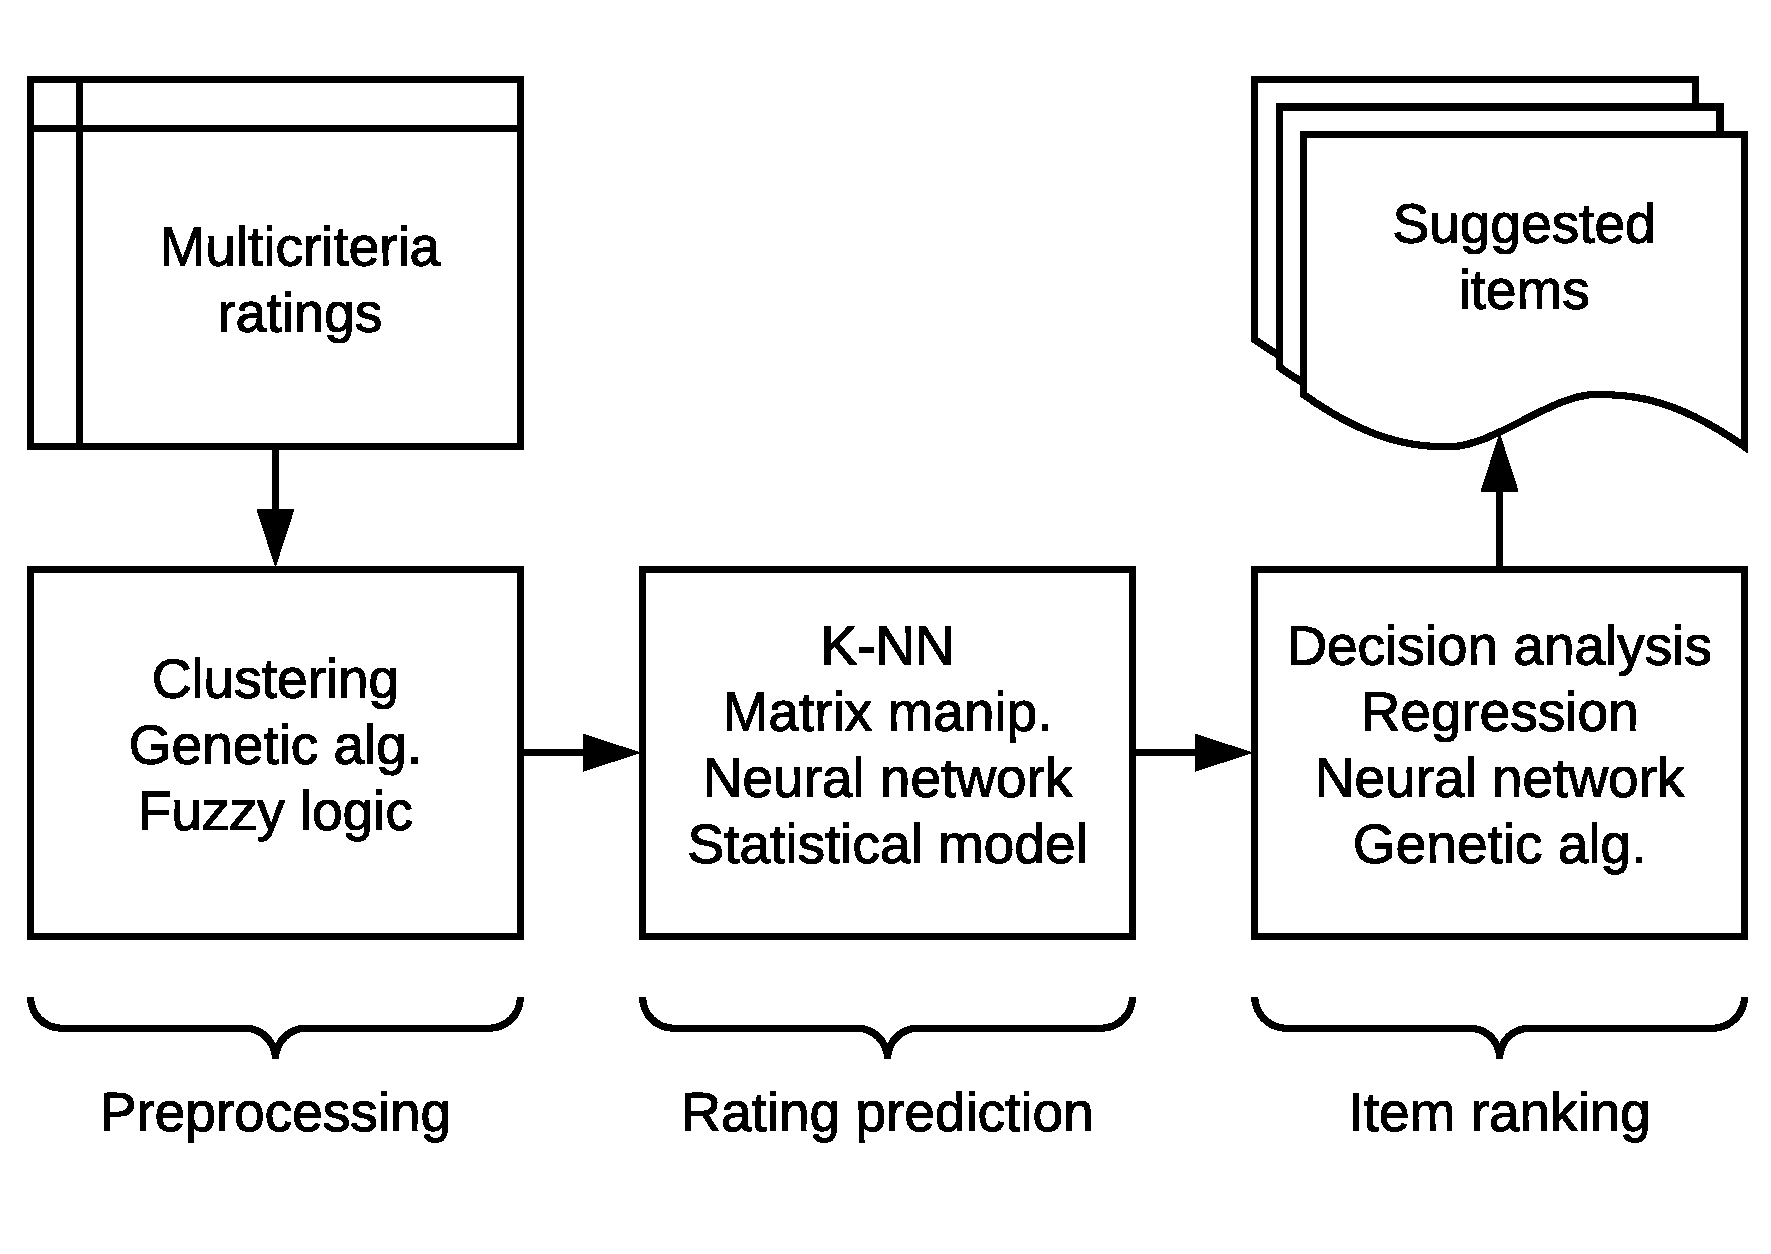
\includegraphics[width=.9\textwidth]{multicriteria_techniques}
\caption[Ideal multicriteria recommender]{This diagram represents the possible techniques exploited by an ideal multicriteria recommender, subdivided according to the recommendation phase. Content-based features and other less common approaches are not considered.}
\label{mcr:fig:techniques}
\end{figure}

\subsection{Application Domains}

As already observed in Section~\ref{mcr:sec:domains}, multicriteria recommenders are frequently exploited in the tourism and travel domain. This result is \added{expected}, as many travel websites, like TripAdvisor\footnote{\url{https://www.tripadvisor.com}} and Bcn Restaurantes,\footnote{\url{https://www.bcnrestaurantes.com}} rely on multicriteria ratings for suggesting items to their users. Even for someone that is not a domain expert, it is possible to identify some useful criteria that should be considered when evaluating a hotel or a restaurant.

For this reason, we can suppose that items belonging to complex domains can be more easily analyzed considering different dimensions and, therefore, they are better suited for multicriteria recommender systems. Another popular example is represented by consumer products, which can be evaluated considering different criteria based on their features, price, and quality.

On the other hand, domains like music or books are usually not exploited for creating a multicriteria recommender, probably because assigning detailed evaluations of such items is too difficult for someone that is not a domain expert.

Another factor that must be considered before performing further analysis is the availability of a certain multicriteria rating dataset in a particular domain. For example, many researchers used to collected ratings from the Yahoo! Movies website, but nowadays such service is no longer available.

The majority of the recommender systems presented in the reviewed studies are domain-independent, as they are only based on multicriteria ratings. However, some solutions designed for specific domains, like medical treatments and research papers, cannot be easily adapted to other scenarios.

\subsection{Evaluation Protocols}

In general, performing the evaluation of a recommender system is a complex task, because the slightest change in the experimental protocol may produce radically different results~\cite{Said2014}. It is not possible to directly compare the outcomes of different works because of the great variety of datasets, evaluation protocols, and metrics mentioned in the reviewed studies.

The multicriteria recommender systems were often evaluated using offline comparisons, as summarized in Table~\ref{mcr:tab:protocols}. This result is \added{expected}, as such \added{an} approach is less expensive \added{than} performing a user study, but it can be used to obtain useful information. However, in order to report more conclusive results, some authors decided to perform a user study. We noticed that it is difficult to involve a significant number of experimental subjects. In fact, only in 3 studies the number of participants was higher than a hundred people.

\subsection{Evaluation Metrics}

The majority of the reviewed studies validated their approach using \added{rating} accuracy metrics, as reported in Table~\ref{mcr:tab:metrics}. This result is probably related to the fact that recommender systems were initially considered as tools designed to predict unknown ratings as accurately as possible. This evaluation approach produces results that are interesting from an academic point of view, but they may have a limited practical meaning.

In fact, as suggested in \cite{Herlocker2000}, it is not possible to display in an application all the items that are associated with the highest predicted ratings. Therefore, it is necessary to be capable of correctly creating lists of ranked items that will be shown to users. This aspect is considered by different studies, in which usage and ranking accuracy metrics are reported.

Other categories of metrics identified during the review include coverage and scalability, which were evaluated in a relatively low number of studies. It is interesting to notice that more recent evaluation dimensions, like diversity, novelty and serendipity, have not been considered, suggesting that their adoption in the recommender system community is still limited.

Finally, we also observed that the differences in the evaluation protocols followed by the reviewed studies do not allow a direct comparison of the results, even when widespread metrics, like MAE or precision, are exploited. \added{For example, we identified a wide variability in the rating dataset, the splitting method between training and test set, and the definition of non-relevant items.} This conclusion is consistent with the findings reported in \cite{Said2014}.

\subsection{Evaluation Datasets}

From the results presented in Section~\ref{mcr:sec:datasets}, we observe that different evaluation datasets have been created using data available in online portals that contain multicriteria ratings. Such collections of ratings are usually not directly provided by the platforms, like the MovieLens datasets, but they are downloaded by researchers using web crawling methods. These approaches result in different versions of the same dataset that sometimes are not publicly available and they can only be obtained by contacting the original creators.

Consider, for example, Yahoo! Movies: this dataset was realized by adding multicriteria ratings to a collection of movie preferences initially provided by Yahoo! Research, quickly becoming one of the most widespread multicriteria gold standards. However, the Yahoo! Movies platform does not provide multicriteria ratings anymore, making impossible to recreate it. Similar observations are also valid for other datasets, as platforms may change over the years and original datasets may become unavailable. \added{Anyway}, we were able to locate two TripAdvisor dataset versions that are still publicly available on the Web.

It is interesting to notice that the authors of different studies decided to create new datasets, relying on real users and simulation tools, or to add additional criteria to existing datasets. This fact suggests that there is the need of realizing and publishing further multicriteria datasets.

\subsection{Future Works}

We described the main future work directions reported by the authors of the reviewed studies in Section~\ref{mcr:sec:future}, in order to identify how it is possible to advance the multicriteria recommender field. The most common suggestion is to add to the proposed technique an additional component for improving its \added{personalization}. The authors of such recommenders usually observe that their methods could benefit from further preprocessing phases or additional components to be combined in a hybrid approach. Another possibility is to consider soft-computing techniques for expressing the uncertainty and vagueness of user ratings.

It is interesting to notice that some studies propose to improve multicriteria recommenders by considering further data, while other authors are more interested in reducing the number of available criteria. These suggestions are not in contrast, as they may be related to the exploited dataset. Therefore, correctly defining the rating criteria and better studying how such ratings are collected are of paramount importance for obtaining high quality recommendations.

Different works propose to also consider friendship relations among users, external knowledge bases and ontologies, and more contextual information. Social Recommender Systems (SRS)~\cite{Guy2015}, Semantics-Aware Recommender Systems (SARS)~\cite{Gemmis2015a}, and Context-Aware Recommender Systems (CARS)~\cite{Adomavicius2015a} are relatively new recommendation approaches that could be exploited jointly with multicriteria techniques in order to create a more personalized experience. However, such additional data need to be managed in a proper way: for this reason, some researchers propose to also study the scalability of the available solutions.

As already discussed, recommender system evaluation is not an easy task. Therefore, different authors declare that they plan to conduct a more extensive experimentation of the proposed approach in future works. This frequent situation may be caused by the difficulties in obtaining multicriteria datasets or by the elevated costs necessary for involving real users in the evaluation process. A related future work is to evaluate the same approach in different domains, as also this suggestion requires further datasets and experiments.

\subsection{Threats to Validity}

In this section, we point out the main problems that we addressed while conducting this systematic literature review. We noticed that there is no strong agreement on a shared definition of multicriteria recommender systems, as there are some subtle differences but also some similarities with multiattribute content-filtering techniques~\cite{Adomavicius2015}. For this reason, we only considered as multicriteria the recommenders based on multicriteria ratings. We also included in our selection few studies describing methods that cannot be considered collaborative filtering approaches, but that exploit multicriteria ratings in a non-conventional way. Furthermore, a limited number of studies were initially selected by analyzing their title and abstract. However, we were later forced to exclude them even if they were potentially relevant because we were not able to retrieve their full-text version. We also noticed that some studies were described in different research papers, and, therefore, we analyzed these situations with attention. Sometimes we selected multiple works because we discovered that these contributions were only partially overlapped.

\section{Conclusion}
\label{mcr:sec:conclusions}

In the context of this systematic literature review, we analyzed a total number of 93 studies related to the topic of multicriteria recommender systems. We provided an answer to nine different research questions, in order to identify which are the main problems that multicriteria recommenders aim to resolve, what recommendation approaches they usually exploit, and what are the most common machine learning and data mining techniques considered for realizing them. Furthermore, we investigated in which domains multicriteria recommenders can be applied, how they are evaluated in terms of experimental protocols, metrics, and rating datasets. Finally, we reported the most common suggestions available in selected studies for conducting future research works.

We identified data sparsity as the most frequent problem that researchers try to address. This issue could be caused by the fact that users are less willing to provide multicriteria ratings because they find this task difficult and time consuming, as they need to consider different aspects of the same item separately. A related research problem is understating what are the most appropriate criteria that should be considered in a particular domain. An excessive number of criteria will most likely result in a partial overlap of their meanings, thus causing a reduction of the prediction accuracy because of the additional noise in the input data. Further studies should better quantify what is the impact of this problem and how recommendation algorithms could reduce it.

We observed that almost all multicriteria recommenders rely on collaborative filtering techniques. This approach is, in fact, also popular in the context of single-criteria recommenders. A large portion of the reviewed studies propose hybrid recommendation methodologies, as they usually combine multiple runs of collaborative filtering algorithms, one for each criterion. However, we also observed a more recent trend of also relying on additional techniques, like content-based, knowledge-based, and community-based approaches. The motivating idea of such recommender systems is to increase the accuracy of the suggested items by exploiting further data behind pure multicriteria ratings.

Furthermore, we classified the machine learning and data mining techniques mentioned in the reviewed studies according to the recommendation phase in which they are considered. We observed that during the preprocessing phase different authors choose to reduce the dimension of the problem inputs by means of clustering and genetic algorithms. In the rating prediction phase, various collaborative filtering methods are considered, like \textit{k}-NN, matrix manipulation techniques, neural networks, and statistical models. Finally, during the ranking phase, it is possible to rely on decision analysis, regression analysis, neural networks, and genetic algorithms. Such methods are combined in various ways, and sometimes integrated with the results of additional recommendation approaches.

We also investigated the domains that are usually considered for implementing a multicriteria recommender system. In the reviewed studies we frequently observed items related to the tourism and travel domain, for example hotels and restaurants. Another popular domain is represented by movies, probably due to the past availability of the Yahoo! Movies datasets. In contrast, domains that are often exploited in single-criteria recommenders, like music or books, are almost never considered for multicriteria approaches. Possible explanations of this finding could be the lack of proper evaluation datasets or the difficulties in defining meaningful criteria and obtaining the associated ratings.

From the analyzed experiments we observed that \added{it} is not possible to directly compare the results obtained with different recommendation approaches due to the extreme variability in the experimental protocols followed by their authors. Another critical point that emerged from this work is the lack of publicly available multicriteria rating datasets. Even if this problem could be partially mitigated with synthetic and crawled datasets, additional efforts should be done in order to \added{create} proper benchmarks in different domains and, thus, enabling a better reproducibility of the experimental results.

Finally, our findings indicate that future works in this field should better explore how to increase the utility of multicriteria recommenders by integrating community-based, knowledge-based, and context-aware approaches, according to the peculiar characteristics of the recommended items. For example, a restaurant recommender system would greatly benefit from context-aware information, a movie recommender could also leverage on semantic data, while a consumer product recommender may assign more importance to the opinions of trusted users. Another interesting point that should be better addressed in future works is defining what are the most appropriate criteria for each domain and how the ratings associated to that criteria should be collected in order to minimize user efforts, also considering soft-computing and linguistic techniques. Furthermore, it would be useful to explore novel algorithms for dynamically understanding the importance that each user implicitly assigns to a criterion, for reducing the fatigue associated with the preference elicitation phase.

\chapter{Evaluation of Sequence-based Recommender Systems}
\graphicspath{{Chapter04/Figures/}}
\label{chap:sequeval}

From the outcome of our systematic literature review on multicriteria recommender systems discussed in Chapter~\ref{chap:multicriteria}, it emerged that traditional approaches usually guarantee interesting results in well-known domains, such as movie recommendation, but they are not capable of capturing the temporal evolution of users' preferences~\cite{Campos2013}. However, different authors~\cite{Ding2005,Rendle2010,He2017} argue that movies watched recently provide more useful information about a certain user than those she consumed in a distant past. It is, in fact, reasonable to assume that a recent item may have a high influence on the choice of the next one.

A recommender system that exploits sequential data for predicting the sole next item that will be consumed by a user can be defined as \emph{sequential recommender}~\cite{Wang2015}. Several works related to sequential recommenders are available in literature, as discussed in Section~\ref{soa:sec:sequential}. For example, Zhou et al.~\cite{Zhou2004} exploited a sequential pattern mining algorithm for recommending which page to visit next in a website, while Rendle et al.~\cite{Rendle2010} relied on Markov chains for suggesting products considering previous purchases. Recently, He et al.~\cite{He2017} designed a recommender system capable of modeling how users' interests evolve over time.

While all these methods usually consider user preferences observed during the training phase as sequences, no temporal ordering is available at recommendation time, as only one item, or a list of items ranked by relevance, is suggested to users. Because of the popularity of CF techniques, most of sequential recommenders are based on such approaches~\cite{Quadrana2018}, but in principle it is also possible to design systems capable of analyzing sequences according to content-based methods.

% Introduce the problem of sequence generation
In general, even if the problem of creating a sequence of words starting from an initial one is a well-known task inside the natural language processing community~\cite{Jurafsky2008}, the idea of creating personalized sequences of items is less widespread in the context of recommender systems~\cite{Herlocker2004}. For this reason, it would be interesting to be able to exploit the temporal ordering not only during the training phase but also for generating sequences of recommended items, such as in the task of language modeling. Some solutions to this problem have already been proposed in industry, and also few researchers have discussed how to automatically construct music playlists~\cite{Chen2012} or suggest sequences of points-of-interest to tourists~\cite{Feng2015} starting from seed items. However, early studies conducted in this field lack of a common definition of the problem that they are trying to address. For example, \emph{session-based} recommenders only consider the last session of the current user~\cite{Ludewig2018}, while \emph{sequence-aware} ones also exploit the history of past sessions~\cite{Quadrana2018} and they can be considered equivalent to sequential recommenders. Furthermore, it is not clear if item repetitions are allowed in the suggestions or not.

In this chapter, we argue that it is possible to consider recommender systems capable of creating personalized sequences of an arbitrary length as a generalization of a sequential recommender because the latter is only able of creating sequences of length \emph{one}. In contrast to traditional approaches that usually create lists of items ranked by relevance, in the following we will define a recommender that exploits a temporal dimension both in the training and in the generation phase as a \emph{sequence-based} recommender, as it observes and suggests sequences of items meant to be consumed in a particular order.

% Evaluation framework for sequence-based recommenders
As discussed in Section~\ref{soa:sec:evaluation}, several evaluation protocols and metrics for analyzing novel recommenders via offline experiments are available, to capture the different aspects of the recommendation algorithm~\cite{Gunawardana2015}. However, the lack of a standardized way of performing such \textit{in vitro} experiments leads to results that are often incomparable~\cite{Jannach2015}. To the best of our knowledge, no evaluation framework for sequence-based recommender systems has already been proposed. Our motivating hypothesis is that, in the context of sequence-based approaches, traditional evaluation metrics need to be computed at the level of sequences instead of the level of users. Therefore, we shift our focus from the multicriteria nature of the input ratings to multicriteria evaluation approaches, that rely on the set of metrics to perform an offline comparison among different recommendation methods.

% Research questions
In our view, an evaluation framework consists of a methodology for performing an experimental comparison, a set of metrics, and a software tool that implements them. The main aim of this chapter is to address the following research questions and to introduce an offline evaluation framework for sequence-based recommender systems that we called Sequeval.

\begin{description}
\item[RQ2.1\label{seq:itm:rq1}] What is the formal definition of a sequence-based recommender system?
\item[RQ2.2\label{seq:itm:rq2}] How already established metrics can be extended and adapted for evaluating a sequence-based recommender system?
\item[RQ2.3\label{seq:itm:rq3}] Against which baseline approaches a sequence-based recommender system can be compared?
\end{description}

Because our evaluation approach is agnostic with respect to the implementation details of the algorithms under analysis, it can be successfully exploited to also assess the performance of systems based on alternative recommendation methods~\cite{Costa2011} or dealing with unconventional categories of items, for example 3D movies~\cite{Pouli2015} or cultural digital contents~\cite{Albanese2011}, especially if they are supposed to be consumed by users in a sequential order. Besides, by openly releasing a Python implementation of Sequeval, we aim to encourage the use of the proposed framework as an attempt to standardize the evaluation of sequence-based recommender systems, mitigating the comparability problem in recommendation research.

The remainder of this chapter is organized as follows: in Section~\ref{seq:sec:sequence-based} we present the mathematical definition of a sequence-based recommender system; in Section~\ref{seq:sec:sequeval} we introduce Sequeval by describing its evaluation protocol, metrics, and implementation details; in Section~\ref{seq:sec:analysis} we perform an empirical analysis of the framework with two datasets. Finally, in Section~\ref{seq:sec:conclusion}, we formulate our conclusions.

\section{Sequence-based Recommender Systems}
\label{seq:sec:sequence-based}

% Definition of rating
Before analyzing the evaluation framework, we introduce the problem of recommending sequences and we provide an answer to \ref{seq:itm:rq1}. In a traditional recommender system, users express positive or negative preferences about a certain item. An item may be, for example, a product, a song, or a place. In contrast, we assume that when a user consumes or interacts with an item, she expresses an implicit rating about it. This assumption in the literature goes under the name of \emph{implicit feedback}~\cite{Herlocker2004}. Because we are also considering the temporal dimension to build the sequences, each rating is associated with a timestamp that represents the point in time when it was recorded.

\begin{definition}
Given the space of items $\mathcal{I}$, the space of users $\mathcal{U}$, the space of timestamps $\mathcal{T}$, a rating $\mathbf{r} \in \mathcal{R}$ is a tuple $\mathbf{r} = (\iota, \upsilon, \tau)$, where $\iota \in \mathcal{I}$ is the item for which the user $\upsilon \in \mathcal{U}$ expressed a positive preference at the timestamp $\tau \in \mathcal{T}$.
\end{definition}

% Definition of sequence
By relying on the set of ratings $\mathcal{R}$ available in the system, it is possible to construct the sequences that will be used to train and to evaluate the recommender. Each sequence only includes the ratings expressed by a single user. On the other hand, each user may produce several sequences.

The concept of \emph{sequence} is similar to the concept of \emph{session} in a traditional web interaction: if two ratings are distant in time more than an interval $\delta \tau$, then they belong to different sequences. Some ratings may be isolated and, for this reason, not part of any sequence. The most appropriate value for $\delta \tau$ depends on the domain: for example, in the POI recommendation scenario, it could be considered of a few hours as reported in \cite{Feng2015}.

\begin{definition}
A sequence $\mathbf{s} \in \mathcal{S}$ is a temporally ordered list of ratings $\langle \mathbf{r}_1,\allowbreak \mathbf{r}_2,\allowbreak \dotsc,\allowbreak \mathbf{r}_n \rangle$ created by a particular user $\upsilon \in \mathcal{U}$, i.e., for each $i$, $\mathbf{r}_i = (\iota_i, \upsilon, \tau_i)$ and $\tau_i < \tau_{i + 1}$.
\end{definition}

In Algorithm~\ref{seq:alg:generate}, we list the procedure for creating the set $\mathcal{S}$, given the set of users $\mathcal{U}$, the set of ratings $\mathcal{R}$, and a time interval $\delta \tau$. Please note that we do not allow the creation of sequences of length \emph{one} because they do not encode a meaningful temporal order.

\begin{algorithm}
\caption{Generation of the set $\mathcal{S}$, given $\mathcal{U}$, $\mathcal{R}$, and $\delta \tau$.}
\label{seq:alg:generate}
\begin{algorithmic}[1]
\REQUIRE $\mathcal{U} \neq \{\emptyset\} \land \mathcal{R} \neq \{\emptyset\} \land \delta \tau \doteq \tau_i - \tau_j$
\STATE $\mathcal{S} \gets \{\emptyset\}$
\FORALL{$\upsilon \in \mathcal{U}$}
\STATE $\mathbf s \gets \varnothing$
\FORALL{$\mathbf r_i \in \mathcal{R}_{\upsilon} : \tau_{i - 1} < \tau_i \land i > 1$}
\IF{$\tau_i < \tau_{i - 1} + \delta \tau$}
\IF{$\mathbf s$ is $\varnothing$}
\STATE $\mathbf{s} \gets \langle \mathbf r_{i - 1} \rangle$
\ENDIF
\STATE $\mathbf{s} \gets \mathbf{s} + \langle \mathbf r_i \rangle$
\ELSE
\IF{$|\mathcal{R}_{\mathbf{s}}| > 1$}
\STATE $\mathcal{S} \gets \mathcal{S} \cup \{\mathbf s\}$
\STATE $\mathbf{s} \gets \varnothing$
\ENDIF
\ENDIF
\ENDFOR
\ENDFOR
\RETURN $\mathcal{S}$
\end{algorithmic}
\end{algorithm}

% Definition of sequence-based recommender
A sequence-based recommender is a recommender system capable of suggesting a personalized sequence that is built starting from a seed rating $\mathbf{r}_0$, considering the example sequences already available in the system and the specific behavior of a certain user. The seed rating is characterized by a seed item $\iota_0$, a target user $\upsilon$, and an initial timestamp $\tau_0$. The seed item can be represented by any item that belongs to the catalog, but, more in general, it is a point in the space of items $\mathcal{I}$. For example, in the music domain, it~could identify not only a particular song, but also an artist, a genre, or a mood. The target user is the user to whom the sequence is recommended, while the initial timestamp represents the point in time in which the recommendation is created. The generated sequence is of a fixed length and it contains exactly $k$ ratings. Please note that if $k = 1$, we are dealing with a sequential recommender as defined in~\cite{Wang2015}.

\begin{definition}
Given a seed rating $\mathbf{r}_0 \in \mathcal{R} : \mathbf{r}_0 = (\iota_0, \upsilon, \tau_0)$, and a length $k \in \mathbb{N}$, a sequence-based recommender is the function $\mathrm{sequence} : \mathcal{R} \times \mathbb{N} \to \mathcal{S}$, i.e., $\mathrm{sequence}(\mathbf{r}_0, k) = \langle \mathbf{r}_1, \mathbf{r}_2, \dotsc, \mathbf{r}_k \rangle : \mathbf{r}_i = (\iota_i, \upsilon, \tau_i)$.
\end{definition}

Most sequence-based recommenders are based on probability models, and therefore they can be interpreted as a sampling function $\sigma$ applied to the conditional probability $P(\langle \mathbf{r}_1, \mathbf{r}_2, \dotsc, \mathbf{r}_k \rangle | \mathbf{r}_0)$:

\begin{equation}
\mathrm{sequence}(\mathbf{r}_0, k) = \sigma (P(\langle \mathbf{r}_1, \mathbf{r}_2, \dotsc, \mathbf{r}_k \rangle | \mathbf{r}_0))
\end{equation}

Using the chain rule, the sequence probability $P(\langle \mathbf{r}_1, \mathbf{r}_2, \dotsc, \mathbf{r}_k \rangle | \mathbf{r}_0)$ can be written as:

\begin{equation}
\label{seq:eq:chainrule}
\begin{split}
P(\langle \mathbf{r}_1, \mathbf{r}_2, \dotsc, \mathbf{r}_k \rangle | \mathbf{r}_0) = & P(\mathbf{r}_k | \langle \mathbf{r}_0, \dotsc, \mathbf{r}_{k - 1} \rangle) \cdot \\ & P(\mathbf{r}_{k - 1} | \langle \mathbf{r}_0, \dotsc, \mathbf{r}_{k - 2} \rangle) \dotsm P(\mathbf{r}_1 | \langle \mathbf{r}_0 \rangle)
\end{split}
\end{equation}

For example, in the case of a Markov chain, each rating depends on the previous one, i.e., $P(\mathbf{r}_k | \langle \mathbf{r}_0, \dotsc, \mathbf{r}_{k - 1} \rangle) =\allowbreak P(\mathbf{r}_k | \mathbf{r}_{k - 1})$:

\begin{equation}
P(\langle \mathbf{r}_1, \mathbf{r}_2, \dotsc, \mathbf{r}_{k} \rangle | \mathbf{r}_0) = P(\mathbf{r}_k | \mathbf{r}_{k - 1}) P(\mathbf{r}_{k - 1} | \mathbf{r}_{k - 2}) \dotsm P(\mathbf{r}_1 | \mathbf{r}_0)
\end{equation}

Thus, a sequence-based recommender system typically works by learning from a set of sequences $\mathcal{S}_{training}$ the conditional probability of the next rating $\mathbf{r}_{k}$ to the sequence of previous ones $\langle \mathbf{r}_0, \mathbf{r}_1 , \dotsc, \mathbf{r}_{k - 1} \rangle$, i.e., the factors of the right-hand side of Equation~\ref{seq:eq:chainrule}.
Sampling sequences directly from Equation~\ref{seq:eq:chainrule} would require computing the probabilities of all the $|I|^k$ possible sequences, where $|I|$ is the size of the vocabulary of items and $k$ is the length of the sequences. Since this becomes easily computationally unfeasible, we opt for a greedy approach, in which at each step we sample the next most likely item. 
A sampling function $\rho$ is defined to select a particular next rating from the previous ones at each step:

\begin{equation}
\mathbf{\hat{r}}_{k} = \rho(P(\mathbf{r}_{k} | \langle \mathbf{r}_0, \mathbf{r}_1, \dotsc, \mathbf{r}_{k - 1} \rangle))
\end{equation}

A trivial example of $\rho$ is the $argmax$ function, which simply selects the most probable next rating. In the following, we will assume that $\rho$ is implemented by a weighted random sampling function.

Algorithm~\ref{seq:alg:recommend} formalizes the procedure for generating a personalized sequence, given a seed rating $\mathbf{r}_0$, and a length $k$, i.e., it describes the sampling function $\sigma$. For $k$ times, the next rating of the recommended sequence is generated using the function $predict$. The function $predict : \mathcal{S} \to \mathcal{R}$ implements the sampling function $\rho$ and it returns the most probable next rating for the current input sequence. In practice, the sequence-based recommender system can estimate the probability that the next rating of the current sequence will include a particular item at a certain timestamp.

Please note that the greedy procedure described in Algorithm~\ref{seq:alg:recommend} is not the only way to create samples of sequences, and thus, the user of the evaluation framework or the designer of the recommendation method are free to define other ways and strategies for that end. 

\begin{algorithm}
\caption{Recommendation of a sequence of length $k$.}
\label{seq:alg:recommend}
\begin{algorithmic}[1]
\REQUIRE $\mathbf{r}_0 \in \mathcal{R} \land k > 0$
\STATE $\mathbf{s} \gets \langle \mathbf{r}_0 \rangle$
\FOR{$i = 1$ \TO $k$}
\STATE $\mathbf{r}_i \gets \mathrm{predict}(\mathbf{s})$
\STATE $\mathbf{s} \gets \mathbf{s} + \langle \mathbf{r}_i \rangle$
\ENDFOR
\RETURN $\mathbf{s} - \langle \mathbf{r}_0 \rangle$
\end{algorithmic}
\end{algorithm}

% Number of items and ratings
To compute some metrics that are part of the evaluation framework, it is necessary to know the number of items that are associated with a certain sequence. For this reason, we define the set $\mathcal{I}_{\mathbf{s}}$ as the set of items that are part of the sequence $\mathbf{s}$, and the set $\mathcal{R}_{\mathbf{s}}$ as the set of ratings that are part of the sequence $\mathbf{s}$. Therefore, $|\mathcal{I}_{\mathbf{s}}|$ is the number of distinct items available in $\mathbf{s}$, while $|\mathcal{R}_{\mathbf{s}}|$ represents the length of $\mathbf{s}$, i.e., the number of ratings available in $\mathbf{s}$.

% Example
For instance, we can suppose that the set of ratings $\mathcal{R}$ is equal to $\{(\iota_1, \upsilon_1, \tau_1),\allowbreak (\iota_2, \upsilon_1, \tau_2),\allowbreak (\iota_3, \upsilon_2, \tau_3),\allowbreak (\iota_1, \upsilon_1, \tau_4),\allowbreak (\iota_2, \upsilon_2, \tau_5),\allowbreak (\iota_3, \upsilon_1, \tau_6)\}$. Then, if we assume that the only pair of timestamps that violates the $\delta \tau$ constraint is $(\tau_4, \tau_6)$, we can create two sequences: $\mathbf{s}_1 = \langle (\iota_1, \upsilon_1, \tau_1),\allowbreak (\iota_2, \upsilon_1, \tau_2),\allowbreak (\iota_1, \upsilon_1, \tau_4) \rangle$, and $\mathbf{s}_2 = \langle (\iota_3, \upsilon_2, \tau_3),\allowbreak (\iota_2, \upsilon_2, \tau_5) \rangle$. The rating $(\iota_3, \upsilon_1, \tau_6)$ is not part of any sequence because it was created at some point in time later than $\tau_4 + \delta \tau$ and we do not have any subsequent rating expressed by $\upsilon_1$. We also observe that $|\mathcal{I}_{\mathbf{s}_1}| = 2$ and $|\mathcal{R}_{\mathbf{s}_1}| = 3$. We would like to recommend a sequence $\mathbf{s}$ of length \emph{two} to user $\upsilon_1$ starting from item $\iota_3$ at timestamp $\tau_{\mathbf{s}, 0}$. In fact, it is not required that the item $\iota_3$ already appeared in the sequences related to user $\upsilon_1$. A possible solution to this problem is to define $\mathbf{r}_{\mathbf{s}, 0} = (\iota_3, \upsilon_1, \tau_{\mathbf{s}, 0})$ and then to recommend $\mathbf{s} = \mathrm{sequence}(\mathbf{r}_{\mathbf{s}, 0}, 2) = \langle (\iota_2, \upsilon_1, \tau_{\mathbf{s}, 1}),\allowbreak (\iota_1, \upsilon_1, \tau_{\mathbf{s}, 2}) \rangle$, where $\tau_{\mathbf{s}, 1}$ and $\tau_{\mathbf{s}, 2}$ may be used to suggest when consuming the items.

\section{Sequeval Evaluation Framework}
\label{seq:sec:sequeval}

Comparing the performance of several recommenders with an experiment that involves a live system is not always feasible or appropriate. For this reason, it is necessary to first perform a preliminary evaluation in an offline scenario~\cite{Gunawardana2015}. In such a setting, we can assess the performance of the algorithms by comparing with baselines, understanding the strengths and weaknesses of those, and thus avoiding affecting real users negatively in their experience with the system. The results of an offline experiment will be less trustworthy than the ones obtained from an online study because there was no real interaction with the system~\cite{Turpin2001}, but they are usually exploited as the first stage in the preparation of the in~vivo experimentation.

Even if an offline study is only the first step in the process of evaluating a recommender, it is necessary to rely on a solid evaluation protocol and a set of well-defined metrics that are able to capture all the characteristics of the analyzed algorithm~\cite{Ge2010}. In the following, we will introduce an offline evaluation framework for sequence-based recommender systems that we called Sequeval.

Our framework is based on the concept of sequence as formalized in Section~\ref{seq:sec:sequence-based}. First, an initial dataset is transformed into a set of sequences following Algorithm~\ref{seq:alg:generate}. Then, the sequences are split between training and test sets. At this point, one or more external recommenders are plugged into the framework: they are exposed to the training sequences and they are asked to create suggested sequences starting from the same seeds of the test ones. A possible strategy for suggesting additional sequences is described in Algorithm~\ref{seq:alg:recommend}, but the user can define other approaches. Finally, considering the recommendations available, the framework can compute different evaluation metrics.

In details, Sequeval is made of an evaluation protocol, presented in Section~\ref{seq:sec:protocol}, a set of evaluation metrics, described in Section~\ref{seq:sec:metrics}, and a software implementation that is introduced in Section~\ref{seq:sec:implementation}.

\subsection{Evaluation Protocol}
\label{seq:sec:protocol}

% Splitting protocol
One of the first problems that an evaluation framework should consider is how to split the dataset between the training set and the test set. This task is not trivial, as it will deeply influence the outcome of the experimentation~\cite{Said2014}. Since we are dealing with sequences, we need to split the set of sequences $\mathcal{S}$ in a training and test set such that $\mathcal{S} = \mathcal{S}_{training} \cup \mathcal{S}_{test}$.

Several solutions to this problem are possible: a simple but effective one is to perform the splitting by randomly assigning sequences to these sets according to a certain ratio, typically the $80\%$ for training and the $20\%$ for testing. If the number of sequences available is limited, it is necessary to perform a cross-validation. Another possibility is to identify an appropriate point in time and to consider all the sequences created before it as part of the training set, and after it as part of the test set. This protocol simulates the behavior of a recommender introduced at that point in time and it avoids too optimistic results caused by the knowledge of future events~\cite{Paraschakis2015}. The latter solution can be considered the most reliable one, but if we do not have any temporal information because the sequences have already been created, it is necessary to adopt a random protocol.

More in general, it is impossible to identify a splitting method that is appropriate for every experiment, as it depends on the domain and on the dataset available. For this reason, Sequeval does not impose the adoption of a particular splitting protocol, but the experimenter can choose the most appropriate one.

% Mathematical notation
To compute the metrics that are part of the evaluation framework, the sequence-based recommender is trained with all the sequences $\mathbf{s} \in \mathcal{S}_{training}$. Then, for each test sequence $\mathbf{s} \in \mathcal{S}_{test} : \mathbf{s} = \langle \mathbf{r}_1, \mathbf{r}_2, \dotsc, \mathbf{r}_n \rangle$, we predict a recommended sequence $\mathbf{\overline{s}}$ of length $k$ using $\mathbf{r}_1 = (\iota_1, \upsilon, \tau_1)$ as seed rating, i.e., $\mathbf{\overline{s}} = \mathrm{sequence}(\mathbf{r}_1, k)$. Therefore, $\mathbf{\overline{s}}$ is a sequence suggested by the recommender, for the same user and starting from the same item of $\mathbf{s}$. We also define $\mathbf{s'}$ as the reference sequence, i.e., $\mathbf{s'} = \langle \mathbf{r}_2, \mathbf{r}_3, \dotsc, \mathbf{r}_n \rangle$ or $\mathbf{s'} = \mathbf{s} - \langle \mathbf{r}_1 \rangle$. The reference sequence is equal to the original sequence, but the first rating is omitted, as it was already exploited for creating the recommended sequence. This procedure is graphically illustrated in Figure~\ref{seq:fig:sequeval-protocol}.

\begin{figure}
\centering
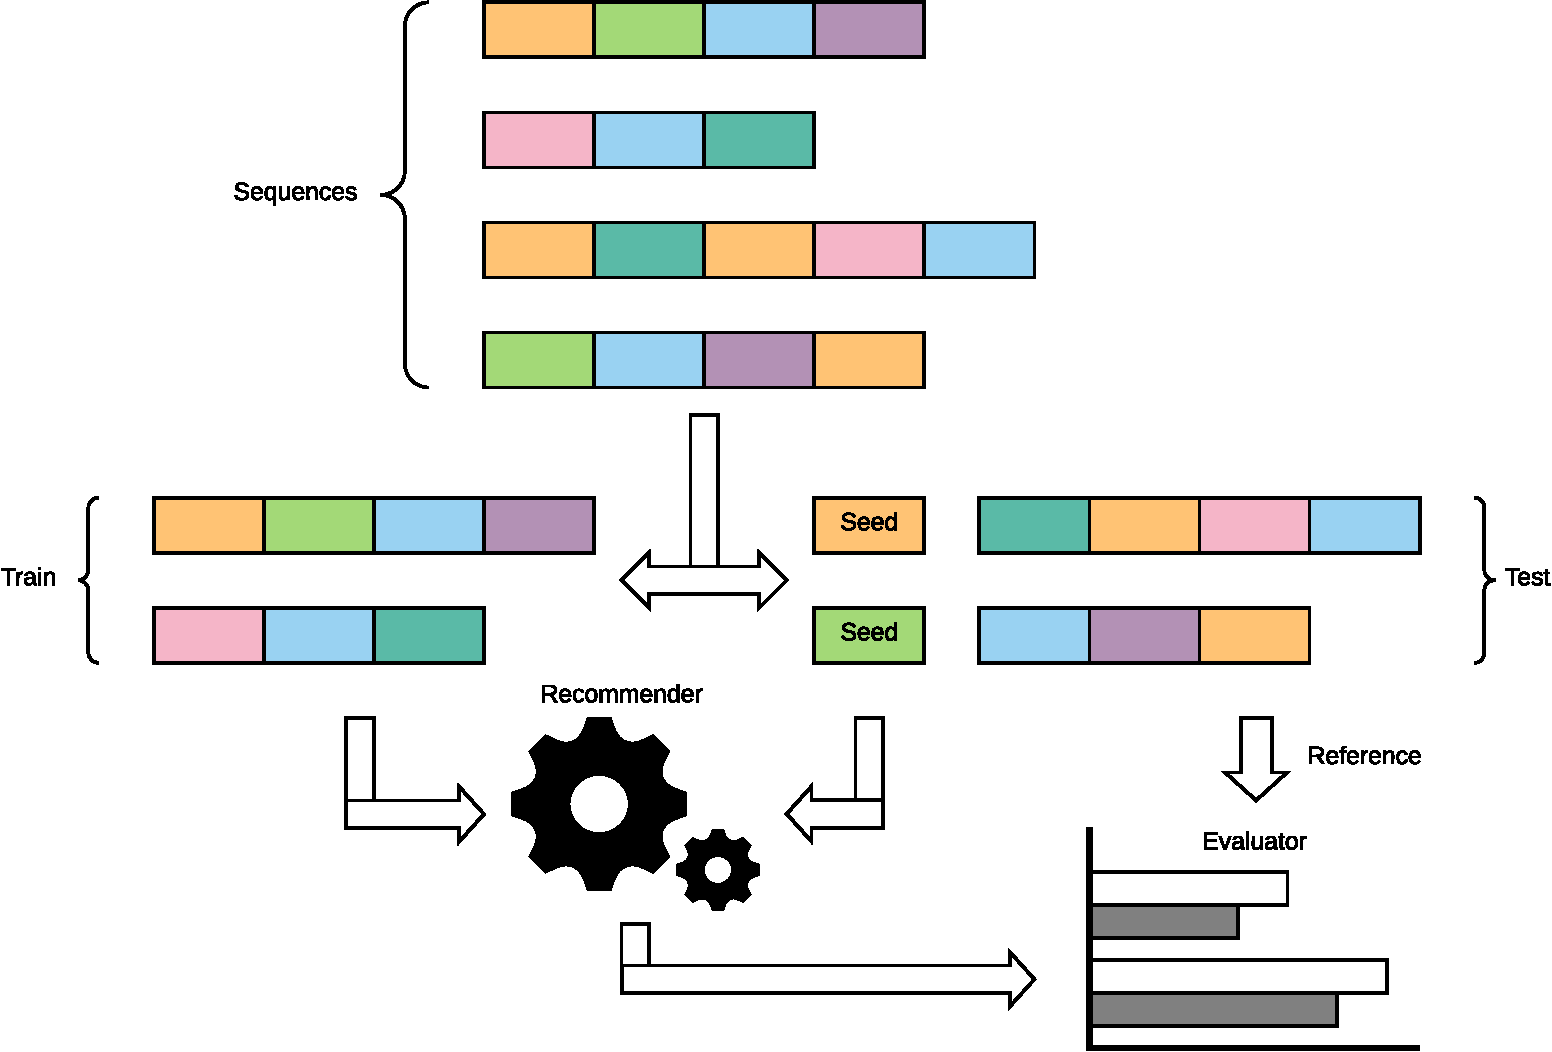
\includegraphics[width=.9\textwidth]{sequeval_protocol.pdf}
\caption[Sequeval evaluation procedure]{An illustration of the evaluation procedure. First, the set of sequences is split between training and test set. Then, the recommender is trained with the sequences available in the training set. Finally, the recommender is asked to generate a sequence for each seed from the test set; such sequences are compared with the corresponding reference sequences.}
\label{seq:fig:sequeval-protocol}
\end{figure}

\subsection{Evaluation Metrics}
\label{seq:sec:metrics}

% General description of the metrics
The second component of Sequeval is a set of eight metrics that we present in the following. In~order to address \ref{seq:itm:rq2}, we include in such set not only classic metrics such as coverage and precision but also less widespread ones such as novelty, diversity, and serendipity. Furthermore, we introduce the metric of perplexity, as it is explicitly designed for characterizing sequences~\cite{Bengio2003}. In contrast, we decided to avoid measuring recall because it is clear that the number of recommended items is often likely to be much lower than the total number of relevant items.

\subsubsection{Coverage}

In general, the coverage of a recommender is a measure that captures the number of items in the catalog over which the system can make suggestions~\cite{Gunawardana2015}. For example, in an online store scenario, it~could represent the percentage of products that are recommended to users in a certain period of time. An algorithm with a higher coverage is generally considered more useful because it better helps users to explore the catalog.

We generate a set of recommended sequences considering as seed the first rating of all sequences in the test set $\mathcal{S}_{test}$ for a recommender that suggests sequences of length $k$. Afterward, we compute the distinct number of items available in the sequences created and we divide the result by the cardinality of the set $\mathcal{I}$.

\begin{equation}
\mathrm{coverage}(k) = \frac{|\bigcup_{\mathbf{s} \in \mathcal{S}_{test}} \mathcal{I}_{\mathrm{sequence}(\mathbf{r}_1, k)}|}{|\mathcal{I}|}
\end{equation}

This metric expresses the percentage of items that the sequence-based recommender can suggest when generating sequences similar to the ones available in the test set and it is strictly related to its cardinality. This approach is similar to the metric of prediction coverage described by Herlocker et al.~\cite{Herlocker2004}.

\subsubsection{Precision}
\label{seq:sec:precision}

Precision is a widespread metric in the context of information retrieval evaluation~\cite{Rijsbergen1979} and it represents the fraction of retrieved documents that are relevant. For a traditional recommender system, precision measures the fraction of recommended items that are relevant for a certain user~\cite{Sarwar2000}. If we consider a sequence-based recommender, it is necessary to compute this metric for each sequence $\mathbf{s} \in \mathcal{S}_{test}$, instead of each user.

\begin{equation}
\mathrm{precision}(k) = \frac{1}{|\mathcal{S}_{test}|} \cdot \sum_{\mathbf{s} \in \mathcal{S}_{test}} \frac{\mathrm{hit}(\mathbf{s'}, \mathbf{\overline{s}})}{\mathrm{min}(|\mathcal{R}_{\mathbf{s'}}|, k)}
\end{equation}

The function $hit : \mathcal{S} \times \mathcal{S} \to \mathbb{N}$ returns the number of items in $\mathbf{\overline{s}}$ that are also available in $\mathbf{s'}$. If the same item is present in $\mathbf{\overline{s}}$ multiple times, it is considered a hit only if it is repeated also in $\mathbf{s'}$. This is an extension to the traditional definition of precision that also considers the fact that an item may appear multiple times inside a sequence.

The number of relevant items is divided by the minimum number between the length of the reference sequence $|\mathcal{R}_{\mathbf{s'}}|$ and the length of the recommended sequence $k$. We decided to adopt this solution to avoid penalizing an algorithm that is evaluated considering reference sequences shorter than the recommended sequences.

\subsubsection{nDPM}

The Normalized Distance-based Performance Metric (nDPM) was originally proposed by Yao in the context of information retrieval~\cite{Yao1995}. The intuition of the author is that in order to compare a system ranking with a reference user ranking, it is necessary to consider all the possible pairs of items available in the system ranking: they can be agreeing, contradictory, or compatible with respect to the user ranking. We decided to adopt such a metric instead of the Normalized Discounted Cumulative Gain (nDCG)~\cite{Jaervelin2002} because, in a sequence of recommendations, it is not necessarily true that the first items are more important than the last ones.

\begin{equation}
\mathrm{nDPM}(k) = \frac{1}{|\mathcal{S}_{test}|} \cdot \sum_{\mathbf{s} \in \mathcal{S}_{test}} \frac{2\,\mathrm{pairs}^-(\mathbf{s'}, \mathbf{\overline{s}}) + \mathrm{pairs}^u(\mathbf{s'}, \mathbf{\overline{s}})}{2\,\mathrm{pairs}(\mathbf{\overline{s}})}
\end{equation}

The function $pairs^- : \mathcal{S} \times \mathcal{S} \to \mathbb{N}$ returns the number of pairs in the sequence $\mathbf{\overline{s}}$ that are in the opposite order with respect to the reference sequence $\mathbf{s'}$. The function $pairs^u : \mathcal{S} \times \mathcal{S} \to \mathbb{N}$ returns the number of pairs in the sequence $\mathbf{\overline{s}}$ for which the ordering is irrelevant, i.e., when at least one of the items is not available in $\mathbf{s'}$ or when at least one of the items is available multiple times in $\mathbf{s'}$. Finally, the function $pairs : \mathcal{S} \to \mathbb{N}$ returns the number of all possible pairs available in the recommended sequence $\mathbf{\overline{s}}$. The pairs are created without considering the ordering of the items inside a pair: for example, if we have the sequence $\langle a, b, c \rangle$, the possible pairs are $(a, b),\allowbreak (a, c),\allowbreak (b, c)$.

The value of this metric will result close to $1$ when the sequences generated by the recommender are contradictory, to $0$ when they have the same ranking, and to $0.5$ when the ordering is irrelevant because they contain different items. A low precision will imply a nDPM very close to $0.5$.

\subsubsection{Diversity}

The metric of sequence diversity included in this framework is inspired by the metric of Intra-List Similarity proposed by Ziegler et al.~\cite{Ziegler2005}. The recommended sequences are considered to be lists of items and the obtained value is not related to their internal ordering. The purpose of this metric is understanding if the sequences contain items that are sufficiently diverse. A higher diversity may be beneficial for the users, as they are encouraged to better explore the catalog~\cite{Noia2014}.

\begin{equation}
\mathrm{diversity}(k) = \frac{1}{|\mathcal{S}_{test}|} \cdot \sum_{\mathbf{s} \in \mathcal{S}_{test}} \frac{\sum_{\forall{i}, \forall{j} : 0 < i < j}^k 1 - \mathrm{sim}(\overline{\iota}_i, \overline{\iota}_j)}{k \times (k - 1)}
\end{equation}

The function $sim : \mathcal{I} \times \mathcal{I} \to [-1, 1]$ is a generic similarity measure between two items. This measure may be taxonomy-driven or content-based: for example, a possible content-based similarity measure is the cosine similarity. The resulting value is a number in the interval $[0, 2]$: higher values represent a higher diversity.

\subsubsection{Novelty}

Vargas et al.~\cite{Vargas2011} suggested that it would be useful to be able to characterize the novelty of the recommendations. They proposed a metric that rewards algorithms capable of identifying items that have a low probability of being already known by a specific user because they belong to the long-tail of the catalog. We have included such metric in our framework to assess whether the items available in the suggested sequences are not too obvious.

\begin{equation}
\mathrm{novelty}(k) = - \frac{1}{|\mathcal{S}_{test}| \times k} \cdot \sum_{\mathbf{s} \in \mathcal{S}_{test}} \sum_{i = 1}^{k} \log_2 \mathrm{freq}(\overline{\iota}_i)
\end{equation}

The function $freq : \mathcal{I} \to [0, 1]$ returns the normalized frequency of a certain item $\iota \in \mathcal{I}$, i.e., the probability of observing that item in a given sequence $\mathbf{s} \in \mathcal{S}_{training}$. We can define the probability of observing the item $\iota$ as the number of ratings related to $\iota$ in the training sequences divided by the total number of ratings available. We also assume that $\log_2(0) \doteq 0$ by definition, to avoid considering as novel items for which we do not have any information, i.e., the items that do not appear in the training sequences.

\subsubsection{Serendipity}

Serendipity can be defined as the capability of identifying items that are both attractive and unexpected~\cite{Gemmis2015b}. Ge et al. proposed to measure the serendipity of a recommender by relying on the precision of the generated lists after having discarded the items that are too obvious~\cite{Ge2010}.

To create a list of obvious items, it is possible to exploit a \emph{primitive} recommender that is a recommender only capable of making obvious suggestions. For example, a primitive recommender could be implemented using the Most Popular (MP) baseline, which is defined in Section~\ref{seq:sec:implementation}. It is reasonable to assume that popular items do not contribute to the serendipity of the recommendations because they are already well known by many users.

By modifying the metric of precision described in Section~\ref{seq:sec:precision}, it is possible to introduce the concept of serendipity in the evaluation of a sequence-based recommender. In this case, the primitive recommender will always create a sequence of length $k$ that contains the items that are have been observed with the highest frequency in the training set.

\begin{equation}
\mathrm{serendipity}(k) = \frac{1}{|\mathcal{S}_{test}|} \cdot \sum_{\mathbf{s} \in \mathcal{S}_{test}} \frac{\mathrm{hit}(\mathbf{s'}, \mathbf{\overline{s}} - \mathbf{\hat{s}})}{\mathrm{min}(|\mathcal{R}_{\mathbf{s'}}|, k)}
\end{equation}

We define $\mathbf{\hat{s}}$ as the sequence generated by the primitive recommender from the same seed of $\mathbf{\overline{s}}$, i.e., $\mathbf{\hat{s}} = \mathrm{primitive}(\mathbf{r}_1, k)$. Moreover, the sequence $\mathbf{\overline{s}} - \mathbf{\hat{s}}$ contains all the ratings related to the items available in $\mathbf{\overline{s}}$ that are not present in $\mathbf{\hat{s}}$. The resulting value will be a number in the interval $[0, 1]$, lower than or equal to precision. The difference between precision and serendipity represents the percentage of obvious items that are correctly suggested.

\subsubsection{Confidence}

The metric of confidence reflects how much the system trusts its own suggestions and it is useful for understanding how robust the learned model is~\cite{Herlocker2000}. It is usually computed as the average probability that the suggested items are correct. This metric expresses the point of view of the recommender, as the probability is reported by the model. Therefore, the metric is always equal to~$1$ with the MP recommender, as it is certain of the predictions.

A sequence-based recommender generates the next item of the sequence by considering all the previous items. For this reason, we can interpret the conditional probability of obtaining a certain item, given the sequence of previous ones, as the confidence that the system has in that suggestion.

\begin{equation}
\mathrm{confidence}(k) = \frac{1}{|\mathcal{S}_{test}| \times k} \cdot \sum_{\mathbf{s} \in \mathcal{S}_{test}} \sum_{i = 1}^k P(\overline{\iota}_i | \overline{\iota}_{i - 1}, \overline{\iota}_{i - 2}, \dotsc)
\end{equation}

We also define $\overline{\iota}_0 \doteq \iota_1$, i.e., the \textit{zero}-th item of the recommended sequence is its seed item. Therefore, this metric is computed by also considering the probability of obtaining the first item $\overline{\iota}_1$, given the seed item of $\mathbf{\overline{s}}$.

\subsubsection{Perplexity}
\label{seq:sec:perplexity}

Perplexity is a widespread metric in the context of neural language modeling evaluation~\cite{Bengio2003}, typically used to measure the quality of the generated phrases. Because there is a strong similarity between creating a sequence of natural language words and sequence of recommended items given an initial seed, perplexity can be also successfully exploited in this context.

This metric can be defined as the exponential in base $2$ of the average negative log-likelihood of the model, i.e., the cross-entropy of the model. For models based on the cross-entropy loss function such as neural networks, the perplexity can also be seen as a measure of convergence of the learning algorithm. Differently from the metric of confidence, the conditional probability $P(\iota_{i + 1} | \iota_i, \iota_{i - 1}, \dotsc)$ is computed considering the items of the test sequence $\mathbf{s}$, and not of the recommended sequence $\mathbf{\overline{s}}$. For this reason, it does not express the point of view of the recommender.

\begin{equation}
\mathrm{perplexity} = 2^{-\frac{1}{\sum_{\mathbf{s} \in \mathcal{S}_{test}} |\mathcal{R}_\mathbf{s}| - 1} \cdot \sum_{\mathbf{s} \in \mathcal{S}_{test}} \sum_{i = 0}^{|\mathcal{R}_\mathbf{s}| - 1} \log_2 P(\iota_{i + 1} | \iota_i, \iota_{i - 1}, \dotsc)}
\end{equation}

Intuitively, the obtained value represents the number of items from which an equivalent random recommender should choose to obtain a similar sequence. The lower is the perplexity, the better is the system under evaluation. Therefore, the perplexity of a random recommender is equal to $|\mathcal{I}|$. If the performance of the recommender is worse than a random one, the perplexity will be higher than $|\mathcal{I}|$: for example, if only one conditional probability is equal to zero, then $\mathrm{perplexity} = +\infty$.

\subsection{Implementation}
\label{seq:sec:implementation}

The third component of Sequeval is \texttt{sequeval}~\cite{Sequeval2018}, a Python implementation of the evaluation framework that is publicly available on GitHub.\footnote{\url{https://github.com/D2KLab/sequeval}} This implementation is based on the protocol presented in Section~\ref{seq:sec:protocol} and it includes the metrics described in Section~\ref{seq:sec:metrics}.

In details, \texttt{sequeval} is a Python package designed following a modular structure, which is graphically represented in Figure~\ref{seq:fig:uml}. For each component, we defined an abstract class and then we realized one or more possible implementations to enable software extensibility.

\begin{figure}
\centering
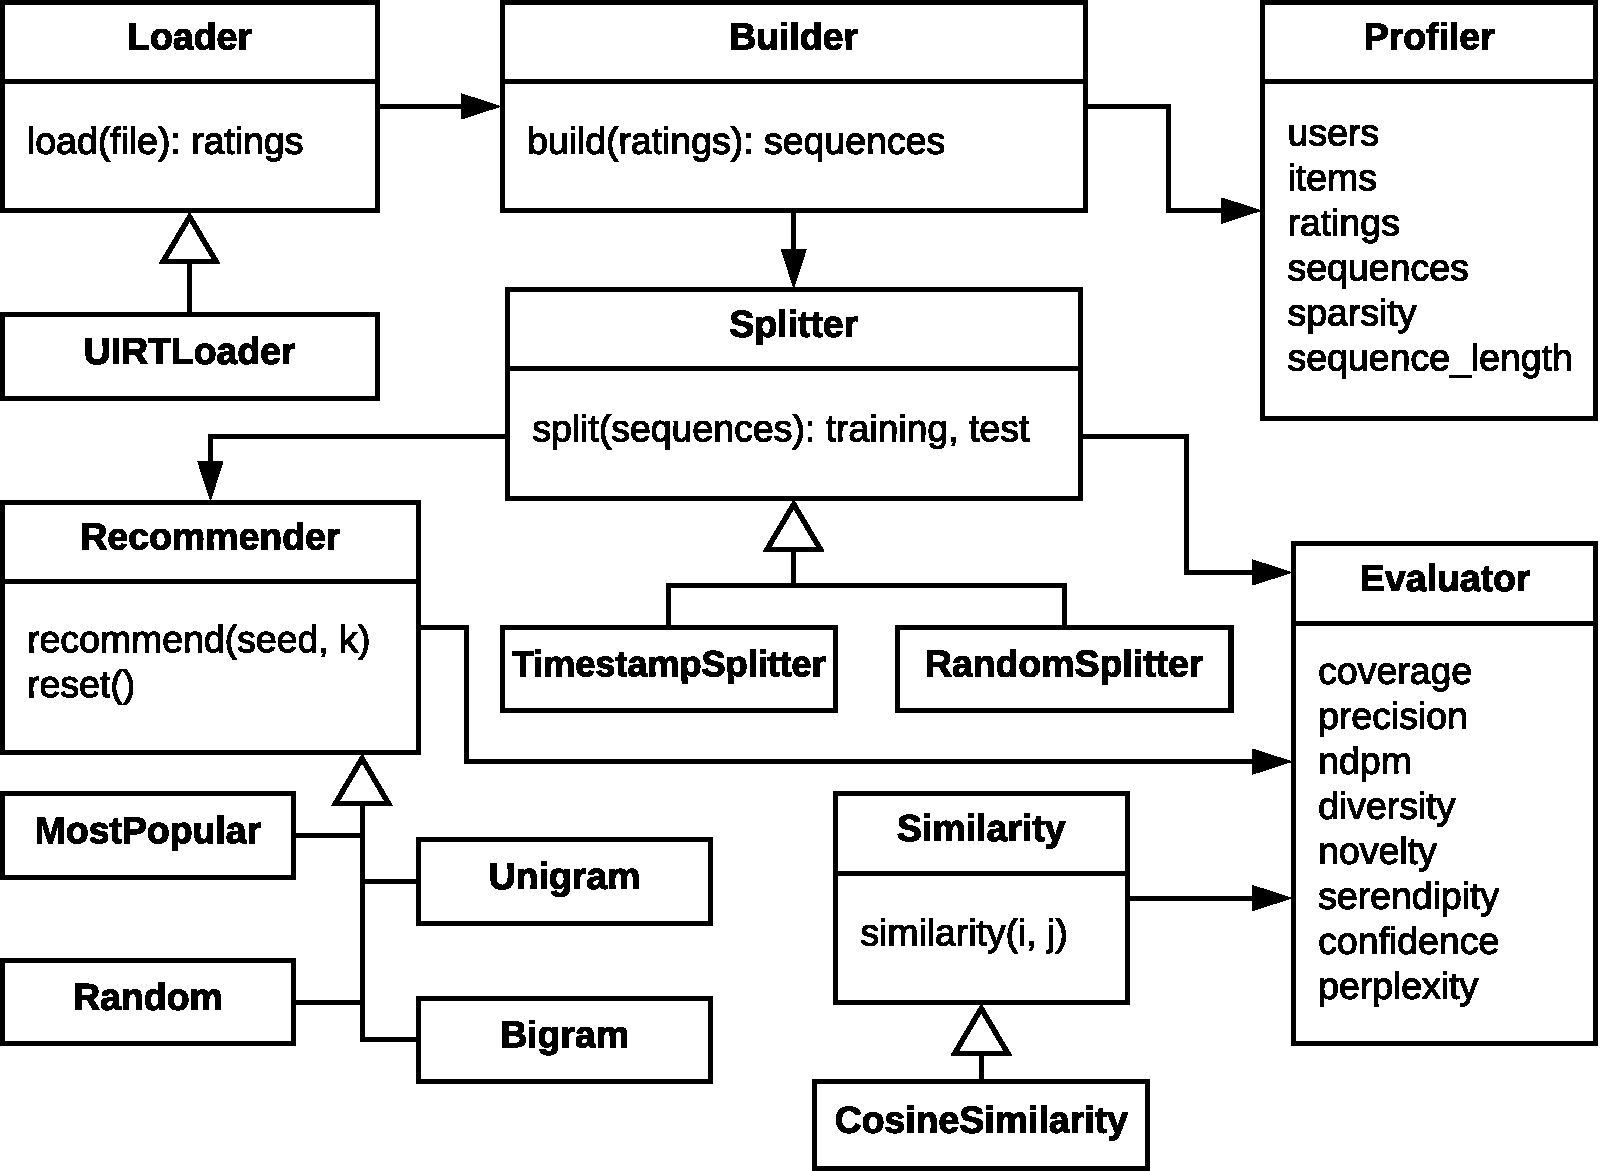
\includegraphics[width=.9\linewidth]{uml}
\caption[UML class diagram of sequeval]{A simplified UML class diagram of \texttt{sequeval}.}
\label{seq:fig:uml}
\end{figure}

The \textit{loader} module is in charge of reading an input file containing user ratings. We have implemented a concrete \textit{loader} capable of processing a textual file in a MovieLens-like format (UIRT), but the support to other formats can be easily added. It is optionally possible to ignore users or items that do not have a minimum number of ratings, in order to avoid data sparsity issues. The \textit{builder} module creates the sequences of items from the initial ratings: ratings from the same user that are distant in time less then a threshold are grouped inside the same sequence. Ratings that do not belong to any sequence are discarded.

The \textit{profiler} module computes some statistics about the generated sequences, for example their average length. The \textit{splitter} module assigns the sequences created by the \textit{builder} to the training and the test sets, according to a random or to a more realistic timestamp-based strategy. It is up to the experimenter deciding the percentage of sequences in the test set.

The \textit{recommender} module includes an abstract class that needs to be implemented by any recommender that relies on this framework, based on the sequence generation logic formalized in Algorithm~\ref{seq:alg:recommend}. The purpose of the abstract class in the \textit{similarity} module is to compute a content-based similarity metric between two items; we have chosen to implement it as a generic cosine-based similarity. Finally, the \textit{evaluator} module computes the measures detailed in Section~\ref{seq:sec:metrics}.

To exploit the proposed framework, it is necessary to realize an implementation of the abstract recommender that must be capable, given the user and the current item of the sequence, of predicting the probabilities for the possible items of being the next one inside the recommended sequence. If the weighted random sampling generation logic is not appropriate, it is possible to override the relative method and to define an alternative recommendation approach.

For obtaining the experimental results, it is necessary to write an evaluation script that relies on this library. We provide a simple evaluation script which can be used to perform different experiments. This script can be easily modified to accommodate novel recommendation techniques.

We also created an extensive test suite achieving the 98\% of code coverage for validating the robustness of our implementation and for better supporting future improvements and developments.% The total development cost of this Python library could be estimated around 40 h.

For demonstrative purposes, we have implemented four baseline recommenders, which are illustrated in the following and represent our answer to \ref{seq:itm:rq3}. These baselines can be interpreted as an adaptation of classic non-personalized recommendation techniques to our sequence-based scenario.

% Baselines
\begin{description}
\item[Most Popular] The MP recommender analyzes the sequences available in the training set to compute the popularity of each item, i.e., the number of times an item appears in the training sequences. Then, at recommendation time, it ignores the seed rating, and it always creates a sequence that contains the MP item as the first rating, the second MP item as the second rating, and so on. More formally, the probability that the item $\iota_i$ will appear in the \textit{i}-th rating of the sequence is $P(\iota_i) = 1$, where $i$ also represents the position of the item in the ranking of the MP ones.
\item[Random] The random recommender simply creates sequences composed of ratings that contain an item randomly sampled from a uniform probability distribution. The seed rating is discarded and the probability of observing the item $\iota_i$ is $P(\iota_i) = 1 / |\mathcal{I}|$, where $|\mathcal{I}|$ represents the number of items available.
\item[Unigram] The unigram recommender can generate sequences that contain ratings with items sampled with a probability proportional to the number of times they were observed in the training sequences. In particular, the probability of observing the item $\iota_i$ is equal to the number of ratings containing $\iota_i$ divided by the total number of ratings available in the training sequences. As with the previous baselines, the seed rating is ignored during the recommendation.
\item[Bigram] The bigram recommender estimates the 1{-st} order transition probabilities among all possible pair of items available in the training sequences. The add-one smoothing technique is exploited to avoid the attribution of a strict zero probability to the pairs that were not observed during the training phase~\cite{Chen1999}. At recommendation time, the seed rating is exploited for selecting the first item, and then each item will influence the choice of the next one. The probability of sampling item $\iota_i$ after item $\iota_{i - 1}$ is equal to the number of times this transition occurred in the training sequences plus one divided by the total number of transitions available.
\end{description}

\section{Experimental Analysis}
\label{seq:sec:analysis}

In this section, we perform an experimental analysis of Sequeval by relying on its implementation described in Section~\ref{seq:sec:implementation} for comparing the behavior of the four baselines with a recommender system based on Conditional Random Fields (CRF)~\cite{Sutton2011} and another one that exploits Recurrent Neural Networks (RNN)~\cite{Goodfellow2016}. The purpose of this comparison is to assess the validity of the framework by conducting an offline evaluation in a realistic scenario. Furthermore, we aim to investigate the efficiency of the proposed approach by analyzing the amount of time required to compute the numerical scores per each recommender system, considering datasets of different sizes.

\subsection{Experimental Setup}
\label{seq:sec:setup}

% Parameters
The main parameters that need to be specified according to our evaluation framework are the $\delta \tau$ value used to generate the sequences, the splitting protocol, and the length of the recommended sequences $k$. The $\delta \tau$ value and the splitting protocol depend on the dataset and they are reported in Section~\ref{seq:sec:datasets}. For performing this empirical analysis, we have decided to exploit the $80\%$ of the dataset for training the recommenders and the remaining $20\%$ for testing purposes. The length of the recommended sequences depends on the specifications of the target application: for this evaluation, we have chosen to set $k = 5$.

% Similarity metric
To compute the metric of diversity, we have selected the cosine similarity among the training sequences as the proximity measure between two items. In fact, we assume that two items are similar if they appear the same number of times inside the same training sequences. Furthermore, we have assumed that if an item is unknown, its similarity with another one is \textit{zero} by definition.

% CRF and RNN
In the following, we provide the rationale for the usage and the implementation details of the two recommenders based on CRF and RNN.

\begin{description}
\item[CRF] We have implemented a CRF-based recommender system using the \texttt{CRFsuite} software package.\footnote{\url{http://www.chokkan.org/software/crfsuite}} Since we are interested in predicting an item given the previous one, we have considered to be feature vectors the training sequences without their last rating and as corresponding output vectors the same sequences without their first rating. We have used the gradient descent algorithm with the L-BFGS method~\cite{Nocedal1980} as the training technique. We have chosen to generate both the state and the transition features that do not occur in the dataset and we have set the maximum number of iterations allowed for the optimization algorithm to $100$.
\item[RNN] We have also experimented with a sequence recommender, originally designed for the tourism domain, based on RNN~\cite{Palumbo2017} that are specifically meant to deal with sequential data. The hyper-parameters of the network have been optimized through a manual search on the validation set in~\cite{Palumbo2017}, obtaining: $\mathrm{n\_layers} = 3$, $\mathrm{dropout} = 0.2$, $\mathrm{learning\_rate} = 0.0001$, $\mathrm{n\_hidden} = 64$, and $\mathrm{n\_epochs} = 10$.
The main difference of RNNs with respect to standard feed-forward neural networks is the presence of a hidden state variable $h_t$, whose value depends both on the input data presented at time $x_t$ and on the previously hidden state $h_{t-1}$~\cite{Goodfellow2016} using loop connections. 
A typical application of RNNs in neural language modeling is the generation of text by recursively applying a ``next word prediction''~\cite{Sutskever2011}. In the same spirit, we address the problem of next item prediction. The probability of the next {rating} given the previous ones $P(\mathbf{r}_{k} | \langle \mathbf{r}_0, \mathbf{r}_1, \dotsc, \mathbf{r}_{k - 1} \rangle)$ is learned during the training process of the neural network without the need for specifying a particular memory window as in Markov models.
\end{description}

For conducting this experimental campaign, we relied on a machine equipped with two 12-cores Intel Xeon processors (E5-2680 v3 at 2.50~GHz) and 128~GB of RAM. However, note that \texttt{sequeval} is a single-threaded application and its memory requirements are actually much lower, around 2.5~GB with the most demanding dataset at our disposal.

\subsection{Datasets}
\label{seq:sec:datasets}

We have performed the experimental analysis considering two different datasets, namely Yes.com and Foursquare. The former is related to the music domain, while the latter deals with check-ins performed at specific POIs.

Because we are interested in modeling sequences, it is important that the temporal information available is actually meaningful. For example, the popular MovieLens datasets~\cite{Harper2015} cannot be exploited for our purposes because the timestamps are associated with the action of assigning a rating on the platform and not with the action of watching a movie. This hypothesis is supported by the fact that, if~we apply Algorithm~\ref{seq:alg:generate} to the MovieLens~1M dataset with $\delta \tau = 1\ \mathrm{h}$, we obtain unrealistic sequences with an average length of about $56$ movies.

The Yes.com and Foursquare datasets are characterized by a different distribution of their items, i.e., songs and venue categories, as it can be observed from Figure~\ref{seq:fig:datasets-barplot}. In particular, Foursquare contains few items that are extremely popular, while Yes.com presents a plot that is smoother. This conclusion is numerically supported by the values of entropy~\cite{Shannon1948} obtained for the two distributions, which are $4.95$ for Foursquare and $6.75$ for Yes.com. Furthermore, the number of sequences available in Foursquare is about $40$ times higher with respect to Yes.com. Table~\ref{seq:tab:datasets-stats} summarizes the number of users, items, ratings, and sequences available in these datasets, which are described in detail in the following sections.

\begin{figure}
\centering
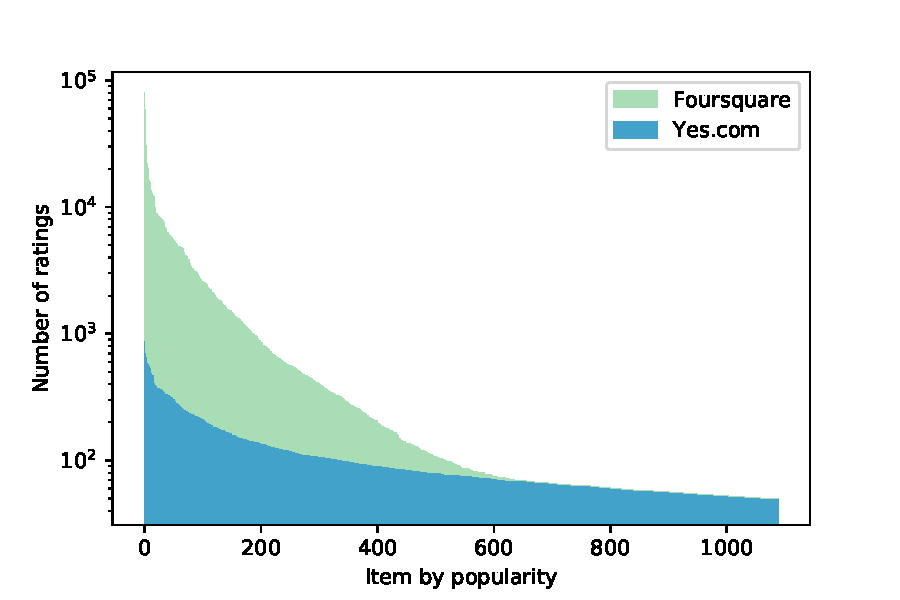
\includegraphics[width=.9\textwidth]{datasets_barplot.pdf}
\caption[Number of ratings per item]{A stacked bar plot with a logarithmic scale representing the number of ratings for each item. Note the different shapes of their long-tail distributions: it is possible to observe that Foursquare has more popular items than Yes.com.}
\label{seq:fig:datasets-barplot}
\end{figure}

\begin{table}
\centering
\begin{tabular}{@{}ccccc@{}}
\toprule
Dataset    & $|\mathcal{U}|$ & $|\mathcal{I}|$ & $|\mathcal{R}|$ & $|\mathcal{S}|$ \\ \midrule
Yes.com    & 1               & 1089            & 118,022         & 10,551          \\
Foursquare & 44,319          & 651             & 1,047,429       & 400,261         \\ \bottomrule
\end{tabular}
\caption[Statistics about the sequences]{The number of users, items, ratings, and sequences after the preprocessing steps. The Yes.com dataset has only one user.}
\label{seq:tab:datasets-stats}
\end{table}

\subsubsection{Yes.com}

This dataset contains several playlists originally collected by Shuo Chen from {Yes.com} in the context of his research on Metric Embedding~\cite{Chen2012}. Such website provided a set of APIs\footnote{\url{http://web.archive.org/web/20150316134941/http://api.yes.com}} for programmatically retrieving songs aired by different radio stations in the United States. By crawling them in the period from December 2010 to May 2011, he managed to obtain $2,840,553$ transitions. Even if {Yes.com} is no longer active, the playlist dataset is publicly available.\footnote{\url{https://www.cs.cornell.edu/~shuochen/lme/data_page.html}}

Yes.com does not include the timestamps, but only the playlists. Therefore, we have assumed that each playlist represents a sequence, as defined in our evaluation framework. In this case, it is not necessary to apply Algorithm~\ref{seq:alg:generate} because the sequences are already available in the dataset in an explicit form. Because a timestamp-based splitting is not feasible, we have selected, for this dataset, a random splitting protocol for dividing the sequences between training and test set.

Since we do not have any information regarding the radio stations, it is necessary to consider the playlists as if they were created by the same user. This approximation is acceptable in the context of sequence recommendation and it is allowed by the evaluation framework. In fact, differently from traditional evaluation approaches, all the metrics that we propose are averaged over the sequences and not over the users. 

Because of the computational complexity of the task, we have randomly reduced the complete dataset $10$ times its original size and we have pruned the songs that appear less than $50$ times.

\subsubsection{Foursquare}

The second dataset that we have selected for performing the experimental evaluation of the framework is similar to the one described in~\cite{Palumbo2017} and it was created following the same protocol.

We collected the check-ins performed by the users of the Foursquare Swarm mobile application\footnote{\url{https://www.swarmapp.com}} and publicly shared on Twitter from the Twitter API. Then, we retrieved the category of the place associated with the check-in thanks to the Foursquare API. For this reason, the items of the dataset are represented by the venue categories available in the Foursquare taxonomy.\footnote{\url{https://developer.foursquare.com/docs/resources/categories}} The collection phase lasted from October to December 2017.

To avoid exploiting the interactions generated by automated scripts, we have discarded the users that performed multiple check-ins in less than one minute. We have also pruned the check-ins associated with the venue categories that are usually not of interest for a tourist, for example the ones related to workplaces. For generating the sequences more efficiently, we decided to also remove the users that have performed less than $10$ check-ins in total.

We have set the $\delta \tau$ parameter of the evaluation framework to $8$ h. Regarding the splitting protocol, we have selected the timestamp-based one, considering the timestamp associated with the first rating as the timestamp of the sequence.

\subsection{Results}

Table~\ref{seq:tab:results-yes} summarizes the figures of the evaluation conducted with Yes.com. The MP recommender achieved a fair precision, but at the price of a very low coverage, because its predictions are deterministic.
Unsurprisingly, the lowest precision and the highest novelty and diversity are associated with the random recommender. In contrast, the unigram, the bigram, and the CRF recommenders obtained comparable scores of precision, but the bigram is the most appealing of these three techniques, because of its lower perplexity and higher novelty.

\begin{table}
\centering
\begin{tabular}{@{}ccccccc@{}}
\toprule
Metric      & MP        & Random & Unigram & Bigram & CRF    & RNN    \\ \midrule
Coverage    & 0.0046    & 1.0000 & 0.9945  & 1.0000 & 0.9991 & 0.9458 \\
Precision   & 0.0503    & 0.0090 & 0.0127  & 0.0103 & 0.0190 & 0.0782 \\
nDPM        & 0.5007    & 0.5000 & 0.5000  & 0.5000 & 0.5000 & 0.4986 \\
Diversity   & 0.6925    & 0.9900 & 0.9815  & 0.9854 & 0.9788 & 0.9052 \\
Novelty     & 7.2383    & 10.380 & 9.7349  & 10.315 & 9.8449 & 9.5762 \\
Serendipity & 0.0000    & 0.0089 & 0.0107  & 0.0095 & 0.0179 & 0.0706 \\
Confidence  & 1.0000    & 0.0009 & 0.0016  & 0.0011 & 0.0020 & 0.0123 \\
Perplexity  & $+\infty$ & 1089.0 & 848.96  & 637.53 & 747.33 & 183.49 \\ \bottomrule
\end{tabular}
\caption[Experimental results with Yes.com]{The results of the baselines and both CRF and RNN with Yes.com.}
\label{seq:tab:results-yes}
\end{table}

We can observe that the RNN recommender achieved the highest precision and the lowest perplexity, resulting to be the most promising algorithm for future online experimentations. Its nDPM is slightly lower than $0.5$, meaning that the items are usually predicted in the correct order. We can also observe that its serendipity is close to the value of precision: for this reason, it is possible to assume that most of the sequences are not obvious.

Table~\ref{seq:tab:results-foursquare} lists, instead, the results obtained with Foursquare. In this case, the MP recommender system accounted for the highest precision, meaning that the top-$5$ items are extremely widespread, but, as usual, its coverage is very limited, and it achieved the lowest novelty. On the other hand, the random recommender scored the lowest precision, and the highest coverage and novelty. The differences among the unigram, the bigram, and the CRF recommenders are more striking than in the previous experiment: with this dataset, the unigram accounted for higher precision because of the popularity of some items, while the bigram for the lowest perplexity.

\begin{table}
\centering
\begin{tabular}{@{}ccccccc@{}}
\toprule
Metric      & MP        & Random & Unigram & Bigram & CRF    & RNN    \\ \midrule
Coverage    & 0.0077    & 1.0000 & 0.9616  & 1.0000 & 0.9677 & 0.5069 \\
Precision   & 0.2259    & 0.0080 & 0.0774  & 0.0607 & 0.0754 & 0.0962 \\
nDPM        & 0.4998    & 0.5000 & 0.4994  & 0.4998 & 0.4993 & 0.4991 \\
Diversity   & 0.9194    & 0.9971 & 0.9616  & 0.9777 & 0.9621 & 0.9469 \\
Novelty     & 4.6056    & 12.300 & 7.1421  & 9.0216 & 7.3710 & 6.8374 \\
Serendipity & 0.0000    & 0.0060 & 0.0256  & 0.0230 & 0.0252 & 0.0365 \\
Confidence  & 1.0000    & 0.0015 & 0.0171  & 0.0140 & 0.0179 & 0.0264 \\
Perplexity  & $+\infty$ & 651.00 & 141.41  & 122.99 & 147.49 & 140.39 \\ \bottomrule
\end{tabular}
\caption[Experimental results with Foursquare]{The results of the baselines and both CRF and RNN with Foursquare.}
\label{seq:tab:results-foursquare}
\end{table}

The RNN recommender system obtained the second-best precision and perplexity, resulting in a good compromise if we are interested in optimizing both these metrics. Its fair coverage and the low value of serendipity are other hints of the fact that the Foursquare dataset contains few items that are very popular: this characteristic was, in fact, learned and exploited by the recommender.

Finally, we report in Table~\ref{seq:tab:results-efficiency} the amount of time needed for computing the previously described evaluation metrics per recommendation algorithm with the Foursquare and Yes.com datasets. We observe that in the worst case, the evaluation framework was able to conduct an experimental campaign in a few hours. The metric of diversity was the most computationally expensive one because of the time needed to compute the cosine similarity. This fact is particularly evident if we consider the seconds spent to evaluate the random recommender with the Foursquare dataset.

\begin{table}
\centering
\begin{tabular}{@{}cccccccc@{}}
\toprule
Dataset & Div. & MP & Random & Unigram & Bigram & CRF & RNN \\ \midrule
Yes.com & Yes & 0.84 & 4.25 & 3.97 & 4.05 & 963.65 & 66.04 \\
Yes.com & No & 0.78 & 1.14 & 0.98 & 1.05 & 865.17 & 60.68 \\
Foursquare & Yes & 15.88 & 1326.31 & 58.64 & 101.73 & 4096.78 & 1223.26 \\
Foursquare & No & 13.75 & 24.63 & 13.05 & 16.78 & 3989.17 & 1194.52 \\ \bottomrule
\end{tabular}
\caption[Time to evaluate the algorithms]{The time in seconds required to evaluate different algorithms with our framework. We do not consider the time for training the CRF and RNN models. To improve the efficiency of the framework it is possible to avoid computing the computationally expensive metric of diversity.}
\label{seq:tab:results-efficiency}
\end{table}

As expected, the baseline recommenders are less demanding with respect to the CRF and RNN models. However, this analysis is beyond the scope of this work, as we are only interested in optimizing the evaluation framework. If we do not consider the metric of diversity, we observe that the time required for the evaluation phase is linear with respect to the size of the dataset.

\subsection{Discussion}

In the following, we will analyze the results of the empirical analysis to justify the answers to the research questions that were provided in Section~\ref{seq:sec:sequence-based} and in Section~\ref{seq:sec:sequeval}. In particular, our main aim is to explain why it is necessary to rely on a multicriteria framework that includes several metrics to evaluate a sequence-based recommender system.

% Why we need items, users, and timestamps
In Section~\ref{seq:sec:sequence-based} we have introduced the concept of rating and we have defined it considering three different elements: an item, a user, and a timestamp. The idea of associating a user with an item is the basic principle of almost every recommender, while the timestamp is necessary in order to introduce a temporal dimension, and, therefore, the possibility of creating and suggesting sequences, as proposed in \ref{seq:itm:rq1}. Nevertheless, we have successfully applied our evaluation framework in an experiment based on the Yes.com dataset, which does not include any user. Even though a {more} general use case has been considered during its formalization, it is possible to also exploit it in other scenarios, still obtaining an interesting picture of the recommenders under evaluation.

% Why so many metrics
As described in Section~\ref{seq:sec:metrics}, our answer to \ref{seq:itm:rq2} is an evaluation framework that includes eight different metrics, capable of capturing the various characteristics of the algorithms available. For~example, even if the precision of the MP recommender system is very high when tested with Foursquare, we can immediately discard it because of its low coverage. In the same way, the interesting values of diversity and novelty achieved by the random recommender are associated with an unacceptable score of perplexity.

In Table~\ref{seq:tab:metrics-interpretation} we present an interpretation of the metrics available in the framework. These descriptions are meant to offer a human understanding of the results of the offline evaluation. It is worth noticing that these metrics consider only some of the properties of a recommender system~\cite{Gunawardana2015}. However, it is our opinion that those properties are the most salient ones that can be analyzed in our context, without realizing a live system.

\begin{table}
\centering
\begin{tabular}{@{}ll@{}}
\toprule
Metric      & Interpretation                                                  \\ \midrule
Coverage    & The percentage of items that are recommended in the evaluation  \\
Precision   & The percentage of items that are correctly recommended          \\
nDPM        & The correctness of the ordering inside the sequences            \\
Diversity   & How diverse are the items inside the sequences                  \\
Novelty     & How unexpected are the recommended items                        \\
Serendipity & The percentage of non-obvious items that are correct            \\
Confidence  & The confidence that the recommender has about its predictions   \\
Perplexity  & How much the recommender is ``surprised'' by the test sequences \\ \bottomrule
\end{tabular}
\caption[Interpretation of the metrics]{A human readable interpretation of the metrics.}
\label{seq:tab:metrics-interpretation}
\end{table}

The different characteristics of the datasets exploited during the empirical analysis are reflected in their respective figures. In particular, while the values of precision obtained by the random recommender in the two experiments are comparable, the figures associated with both MP and unigram methods are dramatically different. This fact suggests that Foursquare contains a few items that are extremely popular, as it was already clear from Figure~\ref{seq:fig:datasets-barplot}.

On the other hand, the RNN recommender obtained, with both datasets, comparable values of precision, but a very different coverage. For this reason, we can suppose that this approach, differently from the CRF recommender, is capable of better adapting itself to the characteristics of the dataset. The~fact that we can draw such {a }conclusion supports the validity of Sequeval.

Furthermore, we have observed that the amount of time required to compute the evaluation metrics is linear with respect to the dataset size, if we do not consider the metric of diversity. In fact, the computational cost of the cosine similarity was too elevated when we analyzed the behavior of the random recommender with a more demanding dataset. However, because of the modular structure of \texttt{sequeval}, it is easy to avoid computing the metric of diversity for such a recommender.

% What are the properties of each baseline
In line with \ref{seq:itm:rq3}, we have described in Section~\ref{seq:sec:implementation} four different baseline recommenders. From the results of the experiments, it is possible to observe that the values obtained by some of them are fixed. For example, the MP recommender will always achieve a serendipity equal to $0$, and a confidence equal to $1$. Its perplexity is usually $+\infty$, if at least one of the recommended sequences is incorrect. The items suggested are, in fact, considered obvious by definition, and the algorithm is certain of the recommendation because its behavior is deterministic. In a similar way, the perplexity of the random recommender is equal to the total number of items available, i.e., $|\mathcal{I}|$, because of the definition of perplexity provided in Section~\ref{seq:sec:perplexity}.

These two baselines are methods commonly exploited in the literature for evaluating recommender systems. Additionally, we have proposed two techniques better suited for the sequence recommendation problem. The unigram recommender is similar to the MP one, but it is non-deterministic, and it obtained a higher novelty. In contrast, the bigram recommender is the most complex baseline, because it considers the previous item to suggest the next one. For this reason, it always achieved the lowest perplexity among the baselines considered.

\section{Conclusion}
\label{seq:sec:conclusion}

% Summary
In this chapter, we have discussed the problem of recommending sequences of items tailored to the needs of a certain user. We have introduced an offline evaluation framework, called Sequeval, capable of handling this novel family of recommender systems in an offline scenario and we have developed an implementation of it that is publicly available on GitHub. We have included in such a framework an evaluation protocol and eight different metrics, to better capture the characteristics of the algorithms considered.

% Empirical analysis
We have performed an empirical analysis of Sequeval by relying on it for conducting a comparison among four baselines, a CRF recommender, and an RNN-based one. The results have highlighted the fact that this framework is flexible, as it can be successfully applied in non-standard recommendation scenarios, such as with Yes.com, and complete, because of the different metrics included that consider several dimensions of the recommended sequences. In addition, we have observed that the RNN recommender system can effectively adapt itself to the characteristics of the training dataset. This conclusion supports the validity of Sequeval as a tool for conducting an offline experimentation.

The formal definitions provided in Section~\ref{seq:sec:sequence-based} have been conceived as an extension of the seminal works on recommenders capable of recommending sequences. For this reason, it is possible to set the length of the recommended sequences to $1$ if we are interested in obtaining a single item. In a similar way, the item included in the seed rating can be exploited in order to set the context of the recommendation, but it can also be ignored if we want a sequence only based on the target user.

\chapter{Evaluation of Top-k Recommender Systems}
\graphicspath{{Chapter05/Figures/}}
\label{chap:reclab}

Different authors have empirically demonstrated that offline evaluation protocols in the context of recommender systems have several weaknesses~\cite{Said2014}. For example, it is widely known that comparing results obtained in different experimental settings should be done with caution, as the slightest difference in the evaluation protocol may result in measures that are totally inconsistent~\cite{Jannach2015}.

Nevertheless, offline experiments are extremely important for comparing a large number of candidate algorithms without sustaining the costs of an online evaluation involving too many human subjects~\cite{Gunawardana2015}. After having pruned the set of available systems, it is however advisable to analyze them in a real environment for obtaining more conclusive results, as discussed in Section~\ref{soa:sec:evaluation}.

In this chapter, we apply the knowledge about multicriteria evaluation we gained from the work presented in Chapter~\ref{chap:sequeval} to the more traditional setting of top-$k$ lists of suggested items. We propose a way of overcoming the problem of comparing offline evaluation results obtained from different recommendation algorithms in heterogeneous settings. To this end, we designed and implemented an open source evaluation framework for top-$k$ prediction methods, called RecLab,\footnote{\url{https://github.com/D2KLab/reclab}} that is capable of interacting with several recommenders using RESTful APIs.

The responsibilities of the evaluator and the recommender are clearly separated because of the distributed architecture of the system. The evaluator is in charge of building a training set, selecting a set of users to whom recommend the items, and computing the evaluation metrics. On the other hand, the recommender must be capable of predicting a list of the most appropriate items for each user, given the information available in the training set.

The configuration parameters of each experiment are left to the user of the toolkit, who is free to choose the dataset, the splitting strategy, the size of the test set, the length $k$ of the recommended lists, and the rating threshold between relevant and irrelevant items. The experiment can be designed and run by simply interacting with a web-based GUI provided by the toolkit. Other researchers can easily plug their recommender systems into the evaluation pipeline by implementing the APIs defined by RecLab and by deploying them on a server. Thanks to this approach, it is possible to compare, in a controlled environment, different algorithms and techniques without necessary disclosing their implementation details. The results of each experiment, along with the respective configuration parameters, are publicly available to support accountability and comparative analyses of the results.

The remainder of this chapter is structured as follows. In Section~\ref{lab:sec:framework} we introduce the main design choices behind our evaluation framework, while in Section~\ref{lab:sec:interaction} we describe how different recommenders can interact with the evaluator. In Section~\ref{lab:sec:metrics} we explain the mathematical details of the metrics computed during the evaluation phase. We present and discuss our results in Section~\ref{lab:sec:results} and, in Section~\ref{lab:sec:conclusion}, we provide the conclusions.

\section{RecLab Evaluation Framework}
\label{lab:sec:framework}

RecLab has been implemented as a distributed web application: its users can setup the experimental environment by simply visiting a web page. This step is crucial for the correct execution of the measurements, as selecting inconsistent or wrong values may lead to results that are extremely difficult to interpret~\cite{Jannach2015}.

In details, the experimenter needs to specify the following parameters before starting an evaluation:

\begin{itemize}
\item the initial rating dataset;
\item the technique used to split the dataset;
\item the size of the training and the test set;
\item the length $k$ of the lists of recommended items;
\item the threshold between negative and positive ratings;
\item the list of recommenders to be evaluated.
\end{itemize}

We included in this evaluation framework three widely used rating datasets: MovieLens 100K,\footnote{\url{https://grouplens.org/datasets/movielens/100k/}} MovieLens 1M,\footnote{\url{https://grouplens.org/datasets/movielens/1m/}} and HetRec LastFM.\footnote{\url{https://grouplens.org/datasets/hetrec-2011/}} The MovieLens datasets are among the most popular recommender systems datasets about movies preferences~\cite{Harper2015}, while the last one is particularly interesting as it contains the number of times each user listened to a specific artist on LastFM~\cite{Cantador2011}. Other datasets can be easily added by editing a configuration file.

We provide two different methods for splitting the rating dataset $\mathcal{R}$ in a training set $\mathcal{R}_{train}$ and a test set $\mathcal{R}_{test}$ such that $\mathcal{R} = \mathcal{R}_{train} \cup \mathcal{R}_{test}$. The first one is a random splitting method that assigns each rating $\rho \in \mathcal{R}$ to the test set or the training set according to a probability specified by the user, that is proportional to the expected size of the test set. In general, this method should be the preferred one when no temporal information is available~\cite{Gunawardana2015}; the default size of the test set is the 20\% of the ratings present in the whole dataset.

A second splitting technique is based on the timestamps associated to the ratings: the whole dataset is ordered from the oldest to the newest rating; then, the first ones are assigned to $\mathcal{R}_{train}$, while the others to $\mathcal{R}_{test}$. This protocol simulates the behaviour of a recommender introduced at a certain point in time in the system. While the HetRec LastFM dataset does not include any timestamp, the MovieLens ones do. However, their values probably do not represent when users watched a certain movie, but when they rated it on the platform.

Another fundamental parameter of the experiment is the length $k$ of the lists of recommended items, as it will deeply influence all the metrics computed by the evaluator. This value should be set according to the number of items that the final application will display to its users. Typical values for this criterion are $5$ or $10$.

The experimenter also needs to specify what is the threshold between negative and positive ratings: only ratings with a value strictly greater than the threshold will be considered \emph{likes} during the evaluation phase. Many recommenders will only analyze positive ratings during the training phase. However, this is beyond the scope of the evaluator, so it is a responsibility of the recommender to properly load the ratings. The most appropriate value for this parameter depends on the dataset: a typical setting for MovieLens datasets is $3$, thus only $4$ and $5$ stars ratings are considered positive. For the HetRec LastFM dataset, as the rating value represents the number of times a user listened to an artist, any small number may be reasonable, including $0$.

For demonstrative purposes, we included in RecLab a set of recommender systems that follow the interaction protocol described in Section~\ref{lab:sec:interaction}. However, anyone is encouraged to implement other techniques for the purpose of evaluating them with this framework. Further recommenders can be added by simply inserting their URIs in a configuration file present in our repository. All available recommenders are then displayed to the experimenter, for letting her select which ones to evaluate.

In details, we have realized the classical most popular and random recommenders. Our most popular recommender is \emph{personalized}: it will never suggest to a certain user items already rated by the same user in the training set. On the other hand, the random recommender will select any item available in the training set with an equal probability.

Furthermore, we have included the MyMediaLite~\cite{Gantner2011} implementations of the Item KNN, User KNN, BPRMF, and WRMF recommender systems using their default settings.\footnote{\url{http://www.mymedialite.net/documentation/item_prediction.html}} BPRMF is a recommendation algorithm based on a Bayesian ranking optimization method~\cite{Rendle2009}, while WRMF is weighted matrix factorization technique~\cite{Hu2008}.

\section{Interaction Protocol}
\label{lab:sec:interaction}

\begin{figure}
\centering
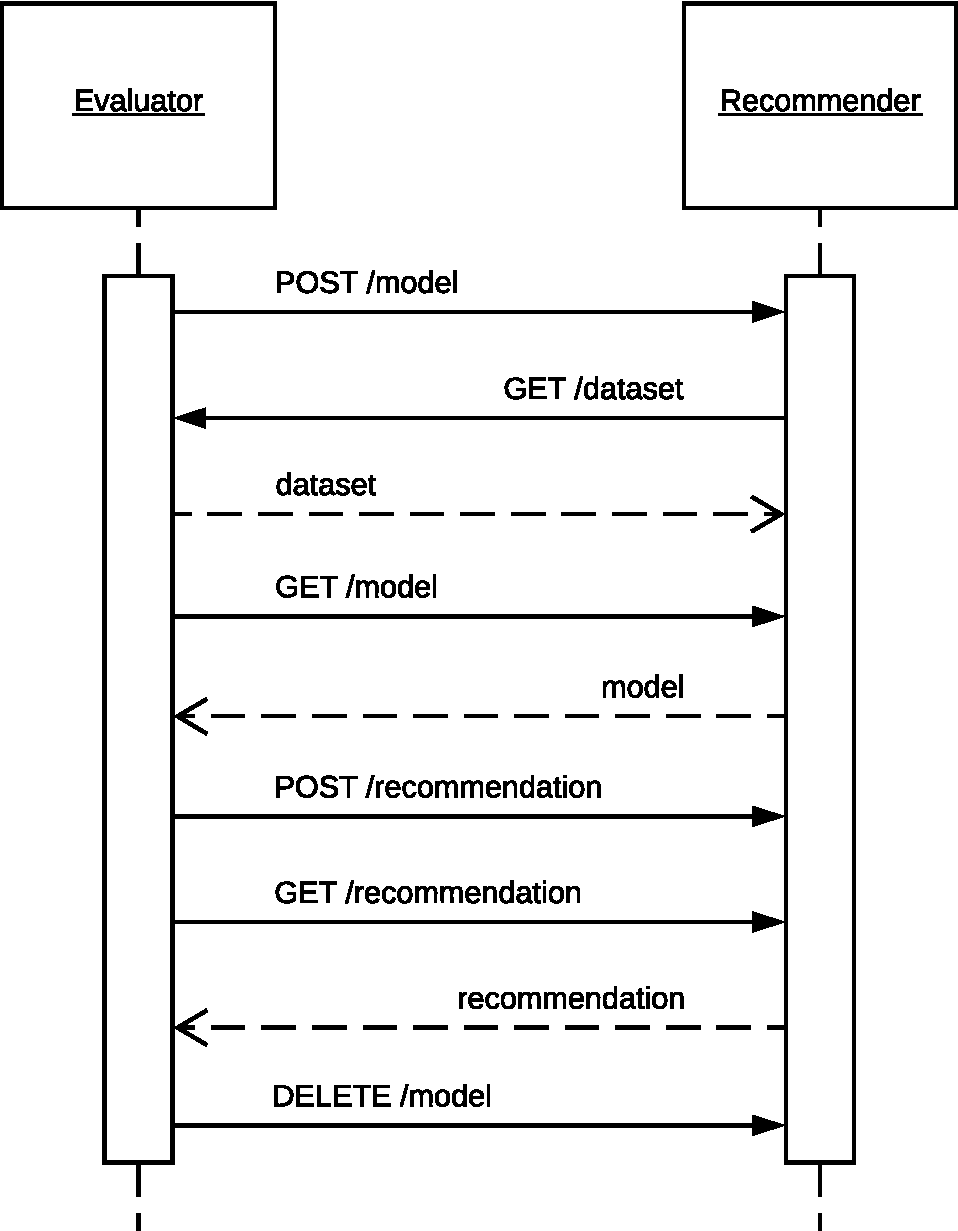
\includegraphics[width=.65\linewidth]{uml}
\caption[RecLab interaction protocol]{A UML sequence diagram describing the RecLab interaction protocol.}
\label{lab:fig:sequence}
\end{figure}

RecLab is a distributed evaluation framework. For this reason, it exploits consolidated web standards to create a communication channel among itself and the recommenders under analysis: the overall protocol is graphically depicted as a UML sequence diagram in Figure~\ref{lab:fig:sequence}. This interaction is initiated when the experimenter decides to execute a new evaluation, and it is repeated for every recommender selected as part of it.

First, the evaluator requests the recommender to train a new recommendation model with a \textsc{post} on the resource \texttt{/model}. It provides to the recommender a URI from which it can download the training set and the rating threshold, as specified by the experimenter. Only the ratings with a value strictly greater than the threshold should be considered as positive feedbacks.

The recommender can now retrieve the training set from the provided URI. Each training set is specific for a particular experiment, but it is created at run time by the evaluator using the configuration settings specified by the user. The training set consists of a list of ratings, where each rating associates a user, an item, and, optionally, a timestamp to a numerical value.

Now the recommender has all the information required to perform the training process. Meanwhile, the evaluator will start asking asynchronously to the recommender if this phase has ended with a \textsc{get} of \texttt{/model}. When the recommender is ready to suggest items, the evaluator is informed of that and it can proceed to the next step.

The evaluator asks the recommender system, with a \textsc{post} on the resource \texttt{/recommendation}, to create a list of $k$ items for each user specified in the payload of the request. The list of users to whom recommend the items contains all the users available in the test set, while the value of $k$ was initially provided by the experimenter. Note that it is a responsibility of the recommender avoiding to suggest items already rated by a particular user in the training set. In general, there is no guarantee that the test set will only contain users and items available in the training set.

Because also the recommendation phase may be time consuming, it is considered asynchronous, similarly to the training one. The evaluator starts asking with a \textsc{get} on the same resource if the lists of recommendations are ready. When they are correctly retrieved, the evaluator asks the recommender to \textsc{delete} the \texttt{/model} to avoid consuming memory, while it begins to compute the evaluation metrics detailed in Section~\ref{lab:sec:metrics}.

\section{Evaluation Metrics}
\label{lab:sec:metrics}

In order to better analyze the recommender systems under evaluation from different perspectives, we decided to include in RecLab a comprehensive set of seven different metrics. In fact, it is not possible to accurately evaluate in an offline experiment a set of recommenders by only relying on a single indicator~\cite{Herlocker2004}. In addition to traditional metrics such as coverage and precision, we propose less widespread ones like novelty, diversity, and serendipity.

% + Recall, nDPM -> NDCG, - Confidence, - Perplexity
These metrics are similar to the ones introduced in Section~\ref{seq:sec:metrics}, but while the latter were designed to evaluate sequences of recommended items, the former are more appropriate for ranked lists of suggestions. We added to RecLab the popular metric of recall, which was not really meaningful in the context of sequence-based recommenders. Furthermore, the metric of nDPM was put aside in favor of NDCG, as it seemed more appropriate to characterize the raking of a list. Finally, we did not consider the metrics of confidence and perplexity, as they would require the recommender systems to also provide a probability for each suggested item, which is beyond the scope of our evaluation framework. This multicriteria set is not final, as RecLab can be easily expanded in order to compute additional metrics that the community considers useful.

In the following, we define $\mathcal{U}$ as the set users $\upsilon \in \mathcal{U}$, $\mathcal{I}$ as the set of items $\iota \in \mathcal{I}$, and $\mathcal{R}$ as the set of ratings $\rho \in \mathcal{R}$. Furthermore, we define $rec(\upsilon, k)$ as the list of the top-$k$ items recommended to user $\upsilon$ and $ref(\upsilon)$ as the set of items rated positively by user $\upsilon$ in the test set $\mathcal{R}_{test}$.

\subsection{Coverage}
The coverage of a recommender is a measure that represents the number of items in the catalog over which the system can make suggestions~\cite{Gunawardana2015}. Given the lists of recommended items for each user in the test set, we compute the percentage of suggested items with respect to the distinct items available in the training set.

\begin{equation*}
\mathrm{coverage}(k) = \frac{|\bigcup_{\upsilon \in \mathcal{U}_{test}} \mathcal{I}_{\mathrm{rec}(\upsilon, k)}|}{|\mathcal{I}_{train}|}
\end{equation*}

This metric captures if the recommender is capable of suggesting enough various items to each user, or if it always proposes the same items to all the users. Coverage should be analyzed together with precision, otherwise it is clear that random recommendations will achieve optimal results~\cite{Herlocker2004}.

\subsection{Precision}
Precision, in the context of information retrieval, represents the fraction of selected documents that are relevant. For a recommender system, it measures the fraction of recommended items that are liked by a user~\cite{Sarwar2000}.

\begin{equation*}
\mathrm{precision}(k) = \frac{1}{|\mathcal{U}_{test}|} \cdot \sum_{\upsilon \in \mathcal{U}_{test}} \frac{|rec(\upsilon, k) \cap ref(\upsilon)|}{k}
\end{equation*}

In order to avoid overestimating the value of precision, we assume that all non-rated items are irrelevant~\cite{Steck2013}.

\subsection{Recall}
Complementary to precision, recall represents the fraction of relevant documents that have been selected. In the context of recommender systems, it measures the fraction of correctly recommended items with respect to all the items the are liked by a user~\cite{Sarwar2000}.

\begin{equation*}
\mathrm{recall}(k) = \frac{1}{|\mathcal{U}_{test}|} \cdot \sum_{\upsilon \in \mathcal{U}_{test}} \frac{|rec(\upsilon, k) \cap ref(\upsilon)|}{|ref(\upsilon)|}
\end{equation*}

If the set of items rated positively by a user is empty, we assume that the recall for that user is $0$ by definition.

\subsection{NDCG}
The Normalized Discounted Cumulative Gain is another information retrieval metric, that also considers a logarithmic gain related to the position of each correctly predicted item~\cite{Jaervelin2002}. This metric reveals if a recommender is capable of correctly predicting items at the top of the list.

\begin{equation*}
\mathrm{dcg}(k) = \frac{1}{|\mathcal{U}_{test}|} \cdot \sum_{\upsilon \in \mathcal{U}_{test}} \sum_{i = 1}^{k} \frac{|\{\iota_i\} \cap ref(\upsilon)|}{log_2(i + 1)}
\end{equation*}

Where $\iota \in rec(\upsilon, k)$. The DCG value needs to be divided by the ideal DCG for normalization. The ideal DCG can be computed with the same formula, assuming that all recommended items are relevant for the associated user.

\subsection{Novelty}
This metric rewards algorithms capable of suggesting items that belong to the long-tail of the catalog, and so it is unlikely that they are already known by a certain user~\cite{Vargas2011}.

In this way, it is possible to check that the recommended items are not too popular and obvious.

\begin{equation*}
\mathrm{novelty}(k) = - \frac{1}{|\mathcal{U}_{test}| \times k} \cdot \sum_{\upsilon \in \mathcal{U}_{test}} \sum_{i = 1}^{k} \log_2 \mathrm{freq}(\iota_i)
\end{equation*}

Where $\iota \in rec(\upsilon, k)$ and $freq : \mathcal{I} \to [0, 1]$ represents the probability of observing the item $\iota$ in $\mathcal{I}_{train}$. We also assume that $\log_2(0) \doteq 0$ by definition.

\subsection{Diversity}
The metric of diversity is inspired by the metric of Intra-List Similarity proposed by Ziegler et al.~\cite{Ziegler2005}. It measures how much the items included in the recommended lists are diverse. A higher diversity may be beneficial for the users, as they are encouraged to better explore the catalog~\cite{Noia2014}.

\begin{equation*}
\mathrm{diversity}(k) = \frac{1}{|\mathcal{U}_{test}|} \cdot \sum_{\upsilon \in \mathcal{U}_{test}} \frac{\sum_{\forall{i}, \forall{j} : 0 < i < j}^k 1 - \mathrm{sim}(\iota_i, \iota_j)}{k \times (k - 1)}
\end{equation*}

Where $\iota \in rec(\upsilon, k)$ and $sim : \mathcal{I} \times \mathcal{I} \to [-1, 1]$ is a similarity measure between two items. We decided to exploit the cosine similarity computed between the vectors representing the users who liked the two items in the training set.

The resulting value is a number in the interval $[0, 2]$: higher values imply an higher diversity.

\subsection{Serendipity}
Serendipity can be defined as the capability of identifying items that are both attractive and unexpected~\cite{Gemmis2015b}. It is possible to measure the serendipity of a recommender by computing its precision after having discarded the items suggested by a \textit{primitive} recommender~\cite{Ge2010}.

\begin{equation*}
\mathrm{serendipity}(k) = \frac{1}{|\mathcal{U}_{test}|} \cdot \sum_{\upsilon \in \mathcal{U}_{test}} \frac{|(rec(\upsilon, k) \setminus prim(k)) \cap ref(\upsilon)|}{k}
\end{equation*}

Where $prim(k)$ is the set of the top-$k$ most popular items available in the training set. We can, in fact, suppose that popular items are already known by several users, and thus they cannot contribute to the serendipity of the suggestions.

\section{Experimental Results}
\label{lab:sec:results}

\begin{sidewaystable}[p]
\centering
\begin{tabular}{@{}llllllll@{}}
\toprule
Algorithm    & Coverage & Precision & Recall   & NDCG     & Novelty  & Diversity & Serendipity \\ \midrule
Random       & 1.000000 & 0.005152  & 0.002526 & 0.005069 & 13.37526 & 0.966485  & 0.005003    \\
Most Popular & 0.017920 & 0.145146  & 0.084294 & 0.158512 & 8.580345 & 0.600524  & 0.071869    \\
Item KNN     & 0.473527 & 0.212028  & 0.137608 & 0.224146 & 10.55504 & 0.788987  & 0.196637    \\
User KNN     & 0.141732 & 0.263337  & 0.189679 & 0.295034 & 9.052157 & 0.657436  & 0.205550    \\
BPRMF        & 0.326907 & 0.225464  & 0.148515 & 0.247625 & 9.473122 & 0.717023  & 0.176972    \\
WRMF         & 0.120554 & 0.258400  & 0.169925 & 0.287808 & 9.138422 & 0.667673  & 0.210835    \\ \bottomrule
\end{tabular}
\caption[Evaluation with MovieLens 1M and random splitting]{Evaluation results with the MovieLens 1M dataset and a random splitting.}
\label{lab:tab:movielens-random}

\bigskip\bigskip

\begin{tabular}{@{}llllllll@{}}
\toprule
Algorithm    & Coverage & Precision & Recall   & NDCG     & Novelty  & Diversity & Serendipity \\ \midrule
Random       & 0.993719 & 0.017555  & 0.002910 & 0.017394 & 13.41860 & 0.963699  & 0.016938    \\
Most Popular & 0.037411 & 0.257487  & 0.053148 & 0.273653 & 8.546251 & 0.528352  & 0.066517    \\
Item KNN     & 0.344894 & 0.231296  & 0.056491 & 0.244158 & 9.759138 & 0.670575  & 0.095962    \\
User KNN     & 0.117422 & 0.275042  & 0.062094 & 0.293720 & 8.842892 & 0.567265  & 0.114470    \\
BPRMF        & 0.220918 & 0.265339  & 0.062845 & 0.282460 & 9.083545 & 0.611382  & 0.112675    \\
WRMF         & 0.136537 & 0.276164  & 0.065600 & 0.297178 & 8.941997 & 0.587175  & 0.121929    \\ \bottomrule
\end{tabular}
\caption[Evaluation with MovieLens 1M and timestamp splitting]{Evaluation results with the MovieLens 1M dataset and the timestamp splitting.}
\label{lab:tab:movielens-timestamp}
\end{sidewaystable}

\begin{sidewaystable}[p]
\centering
\begin{tabular}{@{}llllllll@{}}
\toprule
Algorithm    & Coverage & Precision & Recall   & NDCG     & Novelty  & Diversity & Serendipity \\ \midrule
Random       & 0.708420 & 0.000584  & 0.000632 & 0.000623 & 15.30801 & 0.998417  & 0.000584    \\
Most Popular & 0.001692 & 0.066773  & 0.069242 & 0.076932 & 7.736651 & 0.632728  & 0.019161    \\
Item KNN     & 0.235489 & 0.126168  & 0.131249 & 0.143234 & 12.56312 & 0.774870  & 0.101486    \\
User KNN     & 0.031299 & 0.158652  & 0.164218 & 0.193206 & 8.735683 & 0.717815  & 0.115711    \\
BPRMF        & 0.024597 & 0.078715  & 0.081908 & 0.086609 & 8.280671 & 0.752627  & 0.038800    \\
WRMF         & 0.015617 & 0.164809  & 0.170302 & 0.201023 & 8.849644 & 0.763729  & 0.123992    \\ \bottomrule
\end{tabular}
\caption[Evaluation with LastFM and random splitting]{Evaluation results with the HetRec LastFM dataset and a random splitting.}
\label{lab:tab:lastfm}
\end{sidewaystable}

To prove the effectiveness of RecLab, we performed three different experiments with the recommender systems described in Section~\ref{lab:sec:framework} whose implementation details are available in our repository.

In the first one, we selected the MovieLens 1M dataset and we chose a random splitting protocol. For the other parameters, we used the default values of the framework: the test set size is the 20\% of the dataset, the length $k$ of the recommended lists is equal to $10$, while the rating threshold is equal to $3$. The results of this first experiment are reported in Table~\ref{lab:tab:movielens-random}.

In the second experiment, we changed the splitting protocol to the timestamp-based one, while we retained all other parameters unmodified. The results are reported in Table~\ref{lab:tab:movielens-timestamp}.

Finally, for performing the third experiment, we selected the HetRec LastFM dataset. All other parameters are the same of the first experiment, but the rating threshold, which is now equal to $0$. The results of this last experiment are reported in Table~\ref{lab:tab:lastfm}.

As expected, the random recommender always achieves the best coverage, novelty, and diversity, while also obtaining the worst precision, recall, NDCG, and serendipity. On the other hand, the most popular recommender has a very low coverage and novelty, but it also has interesting values of precision and NDCG, especially with the MovieLens dataset. Note its impressive increase in terms of precision obtained by simply changing the splitting protocol.

The measures of serendipity are not exactly zero because this implementation of the most popular recommender suggests a \emph{personalized} list of popular items, avoiding the ones already rated by the same user in the training set.

If we ignore the random suggestions, the Item KNN recommender obtains the best results in terms of coverage, novelty, and diversity in all the experiments. Regarding the metric of precision, we observe interesting results with the User KNN recommender in the first experiment, with the User KNN and the WRMF in the second one, and with the WRMF in the last one. We observe a dramatic decrease in precision of the BPRMF recommender in the LastFM experiment, probably due to the characteristics of the dataset.

In the last experiment, the WRMF algorithm achieves the best values of precision, recall, NDCG, and serendipity. However, it also scores a very low coverage; in contrast, the Item KNN recommender has a fair precision and an interesting coverage. For this reason, it would be useful to compare these algorithms in an online experiment involving human subjects.

\section{Conclusion}
\label{lab:sec:conclusion}

In this chapter, we have introduced RecLab, an open source framework for evaluating top-$k$ recommender systems in a distributed setting. The main aim of this work is to support the accountability and the reproducibility of the results of the experiments by permanently storing and publicly displaying their configuration parameters and numerical outcomes.

RecLab is based on a RESTful interaction protocol that enables researchers to evaluate different recommenders created with heterogeneous technologies in a common experimental context and with a comprehensive set of metrics.

The results of each experiment can be easily retrieved and automatically processed using a machine-readable format.

We exploited RecLab for performing three experiments involving all the recommenders at our disposal. We empirically validated the importance of considering different metrics in order to execute a reliable evaluation also in the context of top-$k$ recommender systems and we observed the impact of the configuration parameters on the outcome of the experiments.

The scope of this evaluation framework could be expanded by integrating in it more rating datasets and additional recommendation techniques. We also envision the possibility of enhancing the interaction protocol in order to let the experimenter specify the configuration parameters of each recommender.

\chapter{Qualitative Analysis with Rating Datasets Visualization}
\graphicspath{{Chapter06/Figures/}}
\label{chap:rs-viz}

Being able to correctly interpreting the results obtained during an offline evaluation of different recommender systems is of paramount importance for understanding the quality of the suggested items~\cite{Ge2010}. However, this task is particularly difficult as it requires knowing several details regarding the evaluation protocol~\cite{Said2014}. For this reason, in Chapter~\ref{chap:sequeval} and~\ref{chap:reclab}, we have formalized two evaluation frameworks to address the problem of reproducibility in recommender systems research.

In the following, we consider the task of characterizing the rating dataset exploited for conducting the experiments, as it has a profound impact on the final result. For example, sparse datasets usually yield to lower evaluation scores with respect to more dense datasets~\cite{Cremonesi2010}. On the other hand, datasets with many popular items tend to advantage systems that create less diverse suggestions~\cite{Vargas2011}, like the most popular baseline. There are also some subtle differences among rating datasets related to the application domain or the collection protocol that could affect the choice of the most appropriate recommender system.

Different metrics have been proposed in literature to summarize the main characteristic of a rating dataset, i.e. sparsity or entropy. However, we argue that such metrics are not sufficient for comparing datasets in a reliable way, as many other facets should be taken into account. For example, it is not possible to understand the rating behaviors of specific groups of users nor the popularity of the most rated items by only looking at some general statistics computed on the whole dataset.

A possible solution to this problem could be represented by data visualization techniques~\cite{Kunkel2017}. However, most of the methods available in literature are designed to display the output of a recommendation model and not the original dataset~\cite{Gil2018,Cardoso2019}. In contrast, we argue that it is necessary to visually explore a rating dataset even before it is used to train a recommender system, for understanding how the input data will influence the outputs under analysis.

In this chapter, we propose a novel qualitative approach based on data visualization for creating a graphical summary of any collection of user preferences. This method is useful for visually identifying similarities and differences among the available datasets. In fact, we argue that if two datasets result in similar visualizations, the behavior of different recommender systems relying on them will be consistent. Furthermore, we present a Web-based tool, named RS-viz, for easily constructing the proposed visualization and comparing rating datasets in an intuitive way. The software code of RS-viz is freely available on GitHub.\footnote{\url{https://github.com/D2KLab/rs-viz}}

Differently from the plotting capabilities already available in specialized software like Matlab or Scilab, our approach is more general, as it can be applied in a consistent way by different users on any dataset and it can be exploited on many devices without the need of installing specific tools.

\added{More formally, we aim to provide an answer to the following research questions.}

\begin{description}
\item[RQ4.1\label{viz:itm:rq1}] \added{How can data visualization techniques be exploited to create a graphical summary of the main characteristics of a rating dataset?}
\item[RQ4.2\label{viz:itm:rq2}] \added{To what extent the graphical representation of different rating datasets can be useful to easily identify their similarities and diversities?}
\end{description}

The remainder of this chapter is structured as follows. In Section~\ref{viz:sec:visualization} we present the approach used to construct the scatter plot and we describe the implementation details of the Web-based tool RS-viz. In Section~\ref{viz:sec:evaluation}, we comment on the outcome of an evaluation campaign designed to validate the proposed method. Finally, in Section~\ref{viz:sec:conclusion}, we provide the conclusions.

\section{Visualization Approach}
\label{viz:sec:visualization}

In this section, we first describe the algorithm that we devised \added{as an answer to}~\ref{viz:itm:rq1} for creating a scatter plot that represents a rating dataset (Section~\ref{viz:sec:scatter}), then we introduce the implementation details of RS-viz (Section~\ref{viz:sec:implementation}).

\subsection{Scatter Plot Construction}
\label{viz:sec:scatter}

For visually representing the rating matrix associated with a generic dataset we opted for a 3D scatter plot. The rationale behind this choice is that each point in the visualization could intuitively represent a single rating from the dataset: the value of the \textit{x}-axis is the identifier of the user, the value of the \textit{y}-axis is the identifier of the item, while the value of the \textit{z}-axis is the rating itself, if it is expressed on a numerical scale.

However, it is easy to foresee that this approach cannot handle complex datasets with many preferences, as it requires one point for each rating. If the ratings available are only binary, a traditional scatter plot would suffice.

For these reasons, we decided to create a more compact representation of the rating matrix before visualizing it. In details, we first associated the users and the items with internal numerical identifiers according to their frequency of appearance in the dataset. Therefore, we associated the most rated item with the value of~$1$, and the second most rated item with the value of $2$. The same approach was followed for ordering the identifiers of the users according to the number of ratings that they expressed.

Then, we linearly normalized such identifiers within an interval ranging from~$0$ to a user provided value, which represents the size of a squared rating matrix in a transformed space. Finally, we binarized the ratings from the original dataset according to a user provided threshold and we counted, for each cell of the transformed matrix, the number of positive preferences associated with that cell.

For example, if the user $40$ expressed a preference for the item $360$ in a dataset where the number of users is $941$, the number of items is $1446$, and the number of normalized users and items is equal to $100$, that rating would be associated with the cell $(4, 24)$ because $\lfloor 40 \div 941 \times 100 \rfloor = 4$ and $\lfloor 360 \div 1446 \times 100 \rfloor = 24$.

Therefore, the value of the \textit{z}-axis represents the number of positive ratings associated with a sub-matrix of the original dataset, sorted by item popularity and user activity. In order to enhance the readability of the visualization, we also represented the value of the \textit{z}-axis using a logarithmic color scale.

As an example of the proposed method, we report in Figure~\ref{viz:fig:ml-100k} and Figure~\ref{viz:fig:ml-1m} the scatter plots obtained from the MovieLens~100K and MovieLens~1M datasets, when the rating threshold is equal to~$3$, and the number of normalized users and items is equal to $100$.

By looking at the values of the \textit{z}-axis, it is possible to observe in an intuitive way that MovieLens~1M contains a higher number of popular items and of very active users. This conclusion is consistent with the findings of other works that analyze the main characteristics of the MovieLens datasets~\cite{Cremonesi2010}.

\begin{figure}
\centering
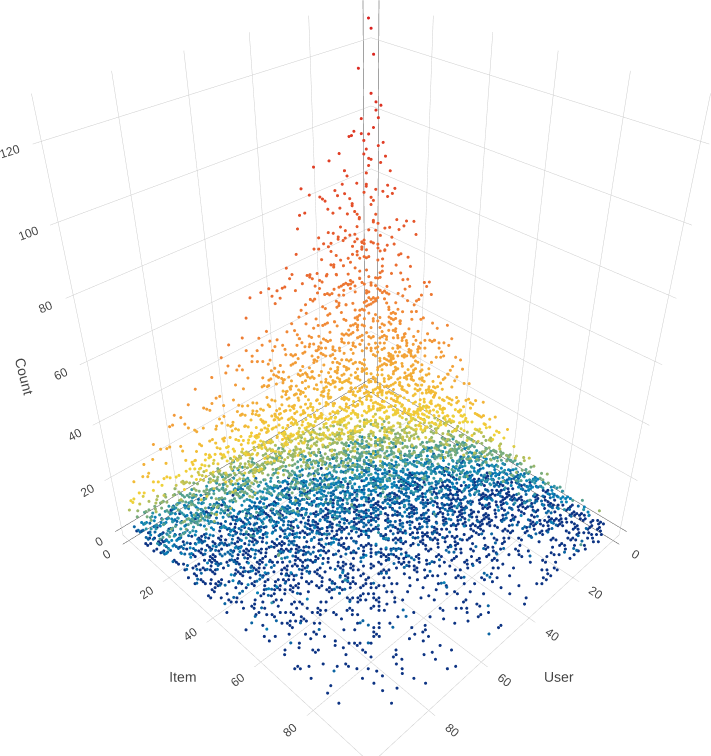
\includegraphics[width=.75\textwidth]{ml-100k}
\caption[Scatter plot of MovieLens~100K]{A scatter plot representing the MovieLens~100K dataset.}
\label{viz:fig:ml-100k}
\end{figure}

\begin{figure}
\centering
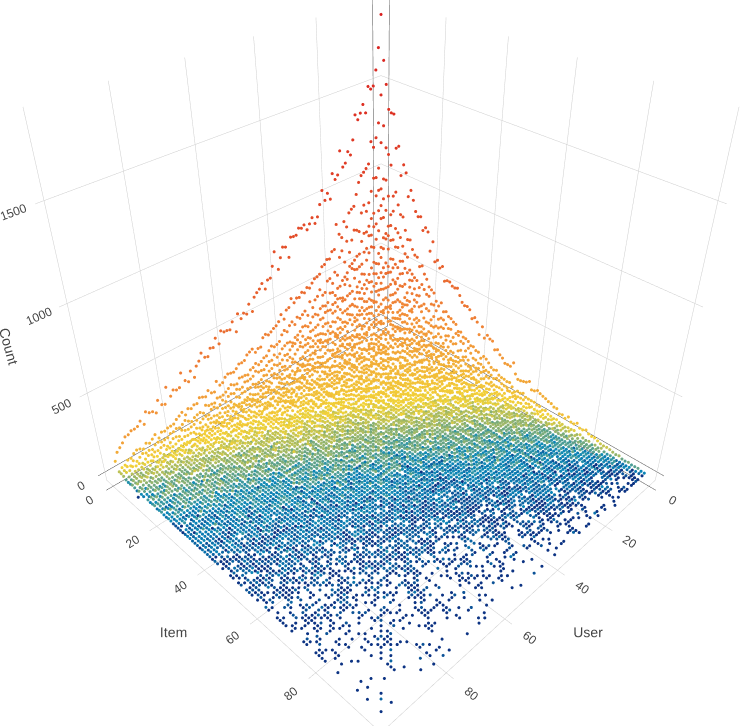
\includegraphics[width=.75\textwidth]{ml-1m}
\caption[Scatter plot of MovieLens~1M]{A scatter plot representing the MovieLens~1M dataset.}
\label{viz:fig:ml-1m}
\end{figure}

\subsection{Software Implementation}
\label{viz:sec:implementation}

We realized a software implementation of the proposed approach as a Web-based tool, called RS-viz, which is freely available. Our visualization framework has been developed using the JavaScript programming language and it runs entirely in a user's browser. For this reason, it can also be exploited for analyzing private datasets, as no information about them is sent to remote servers.

The user needs to visit the Web-page of RS-viz\footnote{\url{https://d2klab.github.io/rs-viz/}} and select one of the built-in datasets or provide her own dataset as a CSV file. Then, she needs to specify the threshold between positive and negative ratings and the number of normalized users and items, which should be selected also considering the rating scale of the input dataset and the desired visualization density. A screenshot of the form containing the configuration parameters of RS-viz is reported in Figure~\ref{viz:fig:rs-viz}.

After a few seconds, an interactive 3D scatter plot is constructed on the right side of the page. The user can inspect the plot by rotating the camera and finally save the result as a PNG file.

\begin{figure}
\centering
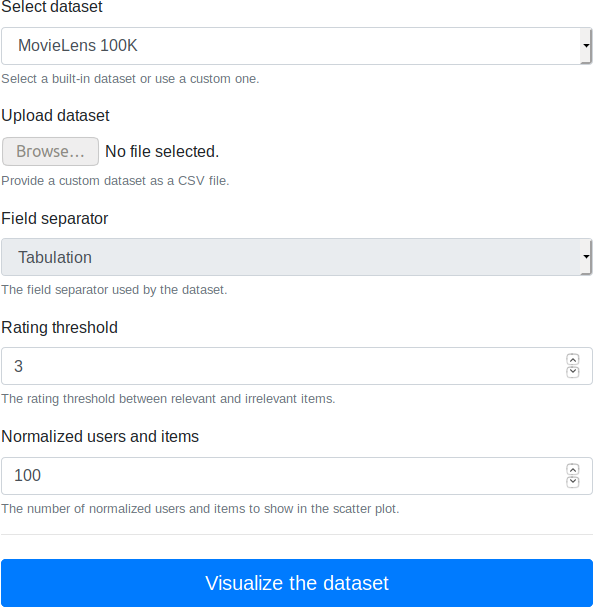
\includegraphics[width=.75\textwidth]{rs-viz}
\caption[Configuration of RS-viz]{The configuration parameters of RS-viz.}
\label{viz:fig:rs-viz}
\end{figure}

\section{Evaluation Campaign}
\label{viz:sec:evaluation}

In the following, we report the numerical outcomes of an evaluation campaign conducted on the HetRec LastFM dataset using different recommendation approaches with the purpose of understanding if our visualization technique is capable of capturing the different characteristics of a rating dataset and to what extent they influence the recommendation coverage and accuracy.

\subsection{Experimental Setup}

We performed two different experiments with the HetRec LastFM dataset and our evaluation framework RecLab, discussed in Chapter~\ref{chap:reclab}.

In the first one, we set the rating threshold equal to 0, while in the second one, we set it equal to 1,000. For the other parameters, we used the default values of the framework: we selected a random splitting protocol, the test set size as the 20\% of the dataset, and the length $k$ of the recommended lists equal to $10$.

We considered different recommendation approaches, namely the most popular and random baselines and the MyMediaLite~\cite{Gantner2011} implementations of the Item KNN, User KNN, BPRMF, and WRMF recommender systems using their default settings.

We computed the metrics of coverage, precision, recall, and nDCG. The results of these experiments are reported in Table~\ref{viz:tab:experiment}. The same datasets obtained from HetRec LastFM by varying the rating threshold were exploited for creating two scatter plots using RS-viz, as displayed in Figure~\ref{viz:fig:lastfm}.

\begin{table}
\begin{subfigure}{\textwidth}
\centering
\begin{tabular}{@{}lllll@{}}
\toprule
Algorithm & Coverage & Precision & Recall & nDCG \\ \midrule
Random & 0.706679 & 0.000798 & 0.000745 & 0.000858 \\
Most Popular & 0.001692 & 0.071170 & 0.071480 & 0.079673 \\
Item KNN & 0.235321 & 0.129362 & 0.131967 & 0.145258 \\
User KNN & 0.030074 & 0.157234 & 0.160353 & 0.193121 \\
BPRMF & 0.022979 & 0.081277 & 0.082248 & 0.094737 \\
WRMF & 0.015558 & 0.159947 & 0.162332 & 0.195107 \\ \bottomrule
\end{tabular}
\caption{Rating threshold = 0}
\bigskip
\end{subfigure}
\begin{subfigure}{\textwidth}
\centering
\begin{tabular}{@{}lllll@{}}
\toprule
Algorithm & Coverage & Precision & Recall & nDCG \\ \midrule
Random & 0.705562 & 0.000107 & 0.000622 & 0.000133 \\
Most Popular & 0.001684 & 0.022122 & 0.090233 & 0.027437 \\
Item KNN & 0.107233 & 0.002878 & 0.013012 & 0.002686 \\
User KNN & 0.049343 & 0.040672 & 0.160767 & 0.055013 \\
BPRMF & 0.003756 & 0.021695 & 0.088211 & 0.024366 \\
WRMF & 0.012886 & 0.039606 & 0.157484 & 0.053148 \\ \bottomrule
\end{tabular}
\caption{Rating threshold = 1,000}
\end{subfigure}
\caption[Experimental comparison with LastFM]{The numerical results of the experimental comparison using the HetRec LastFM dataset.}
\label{viz:tab:experiment}
\end{table}

\begin{figure}
\centering
\begin{subfigure}{.63\textwidth}
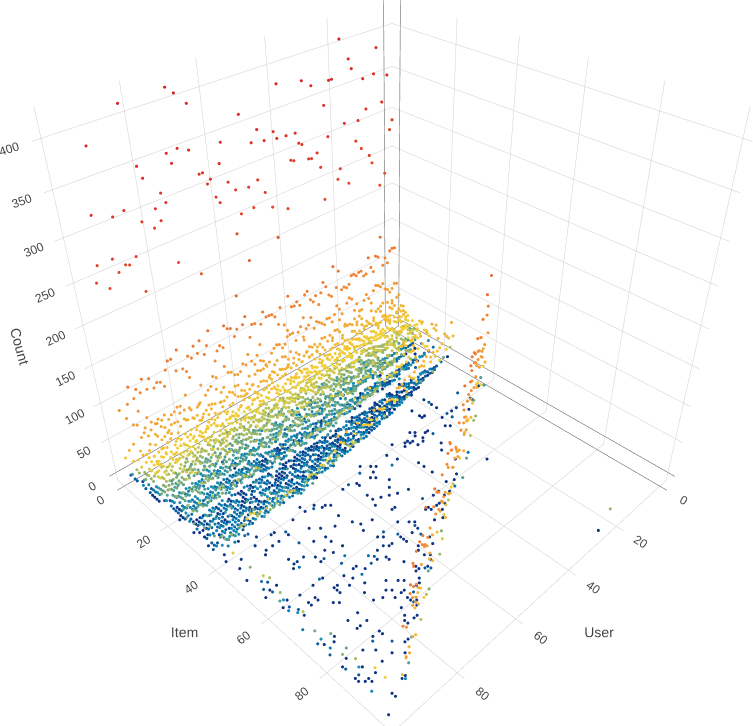
\includegraphics[width=\textwidth]{lastfm-t0}
\caption{Rating threshold = 0}
\label{viz:fig:lastfm-t0}
\bigskip
\end{subfigure}
\begin{subfigure}{.63\textwidth}
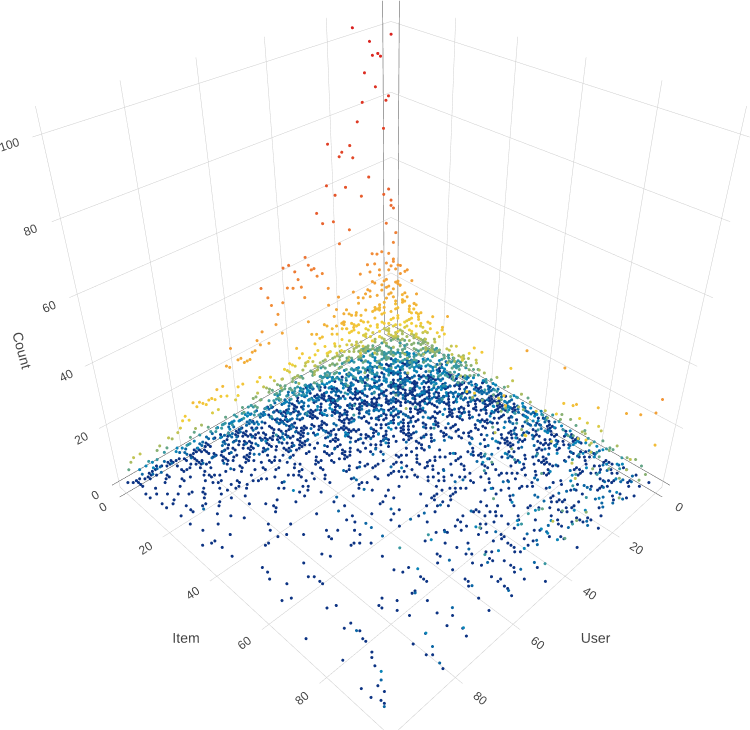
\includegraphics[width=\textwidth]{lastfm-t1k}
\caption{Rating threshold = 1,000}
\label{viz:fig:lastfm-t1k}
\end{subfigure}
\caption[Scatter plots of LastFM]{The scatter plots obtained using the HetRec LastFM dataset with different rating thresholds.}
\label{viz:fig:lastfm}
\end{figure}

\subsection{Discussion}

From the visualization provided in Figure~\ref{viz:fig:lastfm-t0}, we can observe that the HetRec LastFM dataset has a very different structure from the one of the MovieLens datasets. In fact, a limited number of items are associated with the preferences of almost all users, as it can be deduced by considering only the ratings expressed for popular items, that is the ones with low identifiers. Please note that such ratings seem not related to the identifier of the user, resulting in a scatter plot that resembles the shape of a half cylinder.

Furthermore, less popular items seem to be liked by less active users. This behavior can be observed by looking at the lower part of Figure~\ref{viz:fig:lastfm-t0}. Users with a high identifier have rated a more widespread set of items, while users with a low identifier have rated popular items more frequently.

These differences can be easily explained if we consider the collection protocol and the domain of the dataset under analysis. The ratings in the LastFM datasets represent the number of times a user listened to a particular artist: they were collected in an implicit way and their values range from one to tens of thousands.

Also the strange area in the plot with almost no preferences is a direct result of the collection protocol, which relied on the LastFM website to obtain the top artists for a set of users. In fact, the list of artists available in the dataset is limited to $50$ items for each user.

If we increase the value of the rating threshold, we can observe that the resulting scatter plot represented in Figure~\ref{viz:fig:lastfm-t1k} is more similar to the ones of the MovieLens datasets, resulting in a very typical long tail distribution with respect to both the items and the users. This outcome is due to the fact that we removed ratings produced by more casual listeners.

From the numerical outcomes of the experiments, we can deduce that the User KNN and WRMF algorithms are the most appropriate ones with both the different rating thresholds. In general, all the recommenders available perform worse with a higher threshold. In fact, from the visualizations it is clear that the number of available preferences is much lower with respect to the MovieLens~100K dataset, as the scatter plot represented in Figure~\ref{viz:fig:lastfm-t1k} is sparser than the one available in Figure~\ref{viz:fig:ml-100k}. Because user preferences are more limited in number and fragmented, the task of any recommender system is necessarily harder.

Interestingly, the Item KNN, differently from the User KNN, experienced a dramatic drop in all the metrics considered. This result may have been caused by the fact that a very low number of users is available for each item of the dataset. Also this characteristic can be observed from the generated scatter plot by looking at the lower part of Figure~\ref{viz:fig:lastfm-t1k}. The white horizontal stripes denote groups of items that have been rated by only a few very active users.

\added{These experimental results support the validity of our visualization approach and they represent our answer to}~\ref{viz:itm:rq2}.

\section{Conclusion}
\label{viz:sec:conclusion}

In this chapter, we proposed a method for creating graphical summaries of any rating dataset for the purpose of enabling researchers and practitioners to better interpret the results of an offline evaluation campaign. Furthermore, we introduced RS-viz, a Web-based tool capable of creating an interactive 3D scatter plot according to the aforementioned approach starting from a user provided CSV dataset or a built-in collection of ratings.

We validated the capabilities of such visualizations to reveal useful information by comparing the graphical representations of the HetRec LastFM dataset constructed with different rating thresholds with the numerical outcomes of two offline experiments involving various recommendation techniques.

\chapter{Generation and Evaluation of Synthetic Datasets}
\label{chap:synthetic}

It is necessary to rely on a collection of user preferences obtained in a particular domain to perform an offline experiment. For example, the MovieLens datasets represent a popular choice for conducting an offline evaluation in the field of movie recommender systems~\cite{Harper2015}. Nevertheless, the number and the variety of publicly available rating datasets is often limited, especially in less mainstream domains~\cite{Tso2006}. It is possible to identify different causes for this problem. For example, the companies capable of collecting rating datasets are usually reluctant to share them, because of the fear of violating the privacy of their users or of exposing commercially sensible data to their competitors. On the other hand, researchers often do not have the resources for obtaining a sufficient number of ratings that are worth to be publicly released, as discussed in Section~\ref{mcr:sec:datasets}.

Because of the shortage of public datasets, practitioners have started to rely on synthetic ratings in order to conduct their offline experiments~\cite{Yu2012}. An obvious advantage of such an approach is that it enables the creation of rating datasets with an arbitrary number of users and items at a limited cost of dataset acquisition. However, the results obtained from such experiments may be questionable, as the generated datasets are usually not capable of capturing the characteristics of a particular domain of interest~\cite{Montaner2004}. For example, different generative approaches only rely on descriptive statistics, like mean and standard deviation, and, for this reason, they fail to mimic the individual behavior of a user.

In this chapter, we propose a novel approach for automatically generating synthetic datasets with a configurable number of users leveraging on a reference dataset that is used as the seed of the process and that encodes the peculiarities of a domain of interest. Such a generative method can be exploited to create different rating datasets containing users that exhibit behaviors similar to the ones available in the reference dataset. However, the synthetic users do not have a direct relation with the real users and, therefore, no private or commercially sensible information is leaked. At the same time, because the number of synthetic users is configurable, the generated dataset can be exploited to conduct scalability tests in a realistic way and to train recommendation algorithms using reinforcement learning approaches.

More formally, we aim to provide an answer to the following research questions.

\begin{description}
\item[RQ4.3\label{syn:itm:rq1}] What is the impact of using a synthetic dataset instead of a real one on the results of an offline experiment in the context of recommender systems?
\item[RQ4.4\label{syn:itm:rq2}] Can a generative approach be exploited to create a synthetic dataset that exhibits properties similar enough to the ones of a real dataset?
\item[RQ4.5\label{syn:itm:rq3}] To what extend this method can be consistently applied to datasets from different domains and of different sizes?
\end{description}

The remainder of this chapter is structured as follows. In Section~\ref{syn:sec:generation} we introduce the generative approach for creating synthetic datasets, while in Section~\ref{syn:sec:experiments} we describe the experimental setup designed to validate it. We present and discuss the results in Section~\ref{syn:sec:results} and, in Section~\ref{syn:sec:conclusion}, we provide the conclusions.

\section{Dataset Generation}
\label{syn:sec:generation}

Our approach for generating synthetic datasets starting from a reference dataset consists of two steps. In the first one, it is necessary to analyze an existing collection of user preferences in order to obtain an accurate representation of the domain of interest. Then, in the second one, it is possible to exploit such a representation for creating different generated datasets.

We argue that only relying on a few statistical distributions computed empirically at a global level from an existing dataset or specified by a researcher is not sufficient to realistically simulate the individual tastes of human beings~\cite{Montaner2004}. Such methods would lead to the creation of datasets with users having no individual preferences, thus making the task of any recommender system nearly impossible.

For this reason, we included a preliminary clustering phase as part of the first step in order to group the users in a fixed number of communities. The individual rating behaviors, represented by different statistical distributions, are learned for each community and then exploited during the sampling phase.

For simplicity, we assume that each user can only express positive preferences about the items available in the system. However, this approach can also be exploited to simulate datasets with ratings expressed on a more complex scale by repeating these steps for each rating value and then by merging the results.

In the following, we detail the user clustering and distribution learning process (Section~\ref{syn:sec:clustering}) and the rating sampling algorithm (Section~\ref{syn:sec:generate}).

\subsection{User Clustering and Distribution Learning}
\label{syn:sec:clustering}

We represent each user $\upsilon \in \mathcal{U}$ from the reference dataset as a vector with length equal to the number of items $|\mathcal{I}|$. The component $\hat{\upsilon}_i$ of such a vector is equal to~$1$ if the user $\upsilon$ expressed a positive rating $\rho$ about the \textit{i}-th item of the catalog, otherwise it is equal to~$0$.

Given this data structure, we decided to apply the K-means clustering algorithm~\cite{Hartigan1979} to group together users who liked a similar set of items in $K$ different clusters. In the following, we define $\mathcal{C}$ as the set of clusters, therefore $|\mathcal{C}| = K$. The value of $K$ needs to be empirically selected by the experimenter because, in general, it depends on the characteristics of the reference dataset.

Every cluster identifies a different community of users. For generating a dataset similar to the reference one, it is necessary to know how many users belong to each community and what are the item preferences associated with them. More in detail, we create the following empirical distributions from the reference ratings:

\begin{itemize}
\item $P^C$, how users are distributed in $K$ clusters;
\item $P^U_k$, how ratings are distributed in $|\mathcal{U}|$ users for each cluster;
\item $P^I_k$, how ratings are distributed in $|\mathcal{I}|$ items for each cluster.
\end{itemize}

Note that only the first distribution is global, while the second and the third ones are associated with a cluster.% The number of empirical distributions is linear with respect to $K$, apart from a constant.

The distribution $P^C$ represents the probability of assigning a user to a certain cluster and it is computed by counting the number of users per cluster. The distribution $P^U_k$ represents the probability of finding a certain number of ratings per user in the cluster $k$ and it is computed by counting the number of ratings per user. Finally, the distribution $P^I_k$ represents the probability of finding a certain number of ratings per item in the cluster $k$ and it is computed by counting the number of ratings per item.

The user clustering and distribution learning process is formalized in Algorithm~\ref{syn:alg:clustering}. Its output is represented by the previously mentioned distributions.

\begin{algorithm}[ht]
\caption{User clustering and distribution learning, given a reference dataset and the number of clusters.}
\label{syn:alg:clustering}
\begin{algorithmic}[1]
\REQUIRE $\mathcal{U} \neq \{\emptyset\} \land K > 0 \land K \leq |\mathcal{U}|$
\STATE $\mathcal{C} \gets \textrm{K-means}(\mathcal{U}, K)$
\STATE $P^C \gets P(\upsilon \in \mathcal{C}_k)$
\FORALL{$k \in \{1, \dotsc, K\}$}
\STATE $P^U_k \gets P(\rho_{\upsilon} | \upsilon \in \mathcal{C}_k)$
\STATE $P^I_k \gets P(\rho_{\iota} | \iota \in \mathcal{I}_{\upsilon} \land \upsilon \in \mathcal{C}_k)$
\ENDFOR
\RETURN $P^C,\ P^U_k,\ P^I_k$
\end{algorithmic}
\end{algorithm}

\subsection{Rating Sampling}
\label{syn:sec:generate}

Starting from the empirical distributions obtained from Algorithm~\ref{syn:alg:clustering}, it is possible to generate a synthetic dataset by applying to them a sampling function $\sigma$. In the following, we assume that $\sigma$ is the weighted random sampling function.

As previously mentioned, the experimenter can select the number of users available in the generated dataset. This value, called $U$, is an input of the rating sampling algorithm, together with the probability distributions. The synthetic dataset can also have the same number of users available in the reference dataset, that is $U = |\mathcal{U}|$, in order to create a more realistic dataset.

Firstly, each generated user $u$ is assigned to a cluster $k$ from the reference dataset, according to the distribution of users per cluster. Then, the number of ratings $I$ for that user is selected considering the distribution of ratings per user in the cluster $k$. Finally, $I$ items are sampled without replacement ($\hat{\sigma}$) from the distribution of ratings per item in the cluster $k$. Thus, the number of user ratings and her liked items are associated with a particular community of users.

The rating sampling procedure is formalized in Algorithm~\ref{syn:alg:generate}.

\begin{algorithm}[ht]
\caption{Rating sampling, given the required number of users and the distributions computed in Algorithm~\ref{syn:alg:clustering}.}
\label{syn:alg:generate}
\begin{algorithmic}[1]
\REQUIRE $U > 0, P^C, P^U_k, P^I_k$
\STATE $\mathcal{R} \gets \{\emptyset\}$
\FORALL{$u \in \{1, \dotsc, U\}$}
\STATE $k \gets \sigma(P^C)$
\STATE $I \gets \sigma(P^U_k)$
\FORALL{$i \in \{1, \dotsc, I\}$}
\STATE $\rho_{u, i} \gets \hat{\sigma}(P^I_k)$
\STATE $\mathcal{R} \gets \mathcal{R} \cup \{\rho_{u, i}\}$
\ENDFOR
\ENDFOR
\RETURN $\mathcal{R}$
\end{algorithmic}
\end{algorithm}

\section{Experimental Setup}
\label{syn:sec:experiments}

We compared the results obtained from the evaluation of different recommenders conducted on popular datasets typically exploited in literature with the ones computed in the same experimental conditions using various collections of synthetic preferences generated starting from them using multiple techniques.

In fact, we claim that a synthetic dataset can be successfully used during an evaluation campaign if the behavior of the recommender systems under analysis is similar to one that it would be possible to observe with the reference dataset. Thus, almost all the possible pairs of recommenders should exhibit the same relation of order for a given dimension and lead to similar conclusions.

Furthermore, we investigated what is the impact of the parameter $K$ on the results of the evaluation, in order to understand how to empirically select the most appropriate value for it.

In our experiments, we utilized Random, Most Popular, User KNN, BPRMF, and WRMF recommendation algorithms and the metrics of precision, recall, and NDCG as defined in the evaluation framework RecLab discussed in Chapter~\ref{chap:reclab}. Regarding the user preferences, we exploited the binarized versions of the MovieLens~100K, MovieLens~1M, and LastFM~\cite{Cantador2011} datasets. We considered as positive all ratings with a value higher than $3$ for MovieLens and than $0$ for LastFM. We relied on the default values of the evaluation framework for all other experimental parameters: we followed a random splitting protocol with a test set size equal to the $20\%$ of all available ratings and we recommended $10$ items for each test user.

From the aforementioned reference datasets we generated their synthetic versions exploiting the procedure described in Section~\ref{syn:sec:generation}. We considered $U$ equal to the number of users originally available, in order to compare datasets of similar size. Furthermore, we also created three baseline synthetic collections with the same number of ratings by not applying the user clustering phase. All the users of such baselines exhibit the same rating behavior, similarly to the approach described in~\cite{CarmenRodriguez-Hernandez2017}. In Table~\ref{syn:tab:stats}, we report different statistics regarding the baseline, generated, and reference datasets.

\begin{table}
\centering
\begin{tabular}{@{}llrrr@{}}
\toprule
Dataset & Version & Users & Items & Ratings \\ \midrule
MovieLens 100K & Baseline & 942 & 1,374 & 55,375 \\
MovieLens 100K & Generated & 942 & 1,332 & 53,915 \\
MovieLens 100K & Reference & 942 & 1,447 & 55,375 \\ \midrule
MovieLens 1M & Baseline & 6,038 & 3,463 & 575,281 \\
MovieLens 1M & Generated & 6,038 & 3,457 & 584,101 \\
MovieLens 1M & Reference & 6,038 & 3,533 & 575,281 \\ \midrule
LastFM & Baseline & 1,888 & 13,342 & 92,834 \\
LastFM & Generated & 1,892 & 13,442 & 92,510 \\
LastFM & Reference & 1,892 & 17,632 & 92,834 \\ \bottomrule
\end{tabular}
\caption[Statistics about the synthetic datasets]{The total number of users, items, and ratings available in the datasets.}
\label{syn:tab:stats}
\end{table}

\section{Results}
\label{syn:sec:results}

In this section, we first discuss the impact of the number of user communities on the evaluation results, then we present a comparison between exploiting the synthetic and the reference datasets.

\subsection{Number of User Communities}
\label{syn:sec:communities}

\begin{table}
\centering
\begin{tabular}{@{}lrrrr@{}}
\toprule
Dataset & Most Popular & User KNN & BPRMF & WRMF \\ \midrule
K = 5 & 0.088449 & 0.099890 & 0.078768 & 0.091749 \\
K = 10 & 0.095793 & 0.124595 & 0.102805 & 0.111974 \\
K = 50 & 0.098378 & 0.133946 & 0.103243 & 0.133838 \\
K = 100 & 0.102415 & 0.150494 & 0.115587 & 0.149945 \\
K = 200 & 0.099672 & 0.154158 & 0.122538 & 0.164114 \\ \bottomrule
\end{tabular}
\caption[Precision obtained by varying the clusters]{The values of precision obtained with the synthetic versions of the MovieLens~100K dataset by varying $K$.}
\label{syn:tab:clusters}
\end{table}

For studying what is the impact of the value $K$ on the results of an evaluation conducted with a synthetic dataset, we computed the measure of precision on different synthetic versions of the MovieLens~100K dataset created with $K = \{5,\ 10,\ 50,\ 100,\ 200\}$. We report the numerical outcomes of this experiment in Table~\ref{syn:tab:clusters}.

We also observed that it is possible to obtain similar results by considering other datasets and metrics. As expected, the values of precision for all the algorithms but the Random and Most Popular approaches improve by increasing the number of available clusters. However, this relationship is not linear, as doubling its value from $100$ to $200$ only slightly improves the results.

We empirically observed that reasonable values for $K$ could be $100$ or $200$. In Section~\ref{syn:sec:datasets}, we will assume that $K = 200$.

Therefore, we can provide an answer to \ref{syn:itm:rq1} by observing that the impact of using a synthetic dataset in an evaluation campaign can be mitigated if we are able to simulate a sufficient number of heterogeneous user communities.

\begin{table}
\begin{subfigure}{\textwidth}
\centering
\begin{tabular}{@{}llll@{}}
\toprule
Algorithm & Precision & Recall & NDCG \\ \midrule
Random & 0.009416 & 0.008877 & 0.009841 \\
Most Popular & 0.060065 & 0.053209 & 0.064384 \\
User KNN & 0.055952 & 0.050587 & 0.058744 \\
BPRMF & 0.045346 & 0.033628 & 0.048740 \\
WRMF & 0.047078 & 0.042876 & 0.048104 \\ \bottomrule
\end{tabular}
\caption{Baseline dataset}
\bigskip
\end{subfigure}
\begin{subfigure}{\textwidth}
\centering
\begin{tabular}{@{}llll@{}}
\toprule
Algorithm & Precision & Recall & NDCG \\ \midrule
Random & 0.009847 & 0.008977 & 0.010022 \\
Most Popular & 0.099672 & 0.083875 & 0.110229 \\
User KNN & 0.154158 & 0.135917 & 0.169499 \\
BPRMF & 0.122538 & 0.106186 & 0.129742 \\
WRMF & 0.164114 & 0.144272 & 0.173916 \\ \bottomrule
\end{tabular}
\caption{Generated dataset}
\bigskip
\end{subfigure}
\begin{subfigure}{\textwidth}
\centering
\begin{tabular}{@{}llll@{}}
\toprule
Algorithm & Precision & Recall & NDCG \\ \midrule
Random & 0.007743 & 0.006300 & 0.008183 \\
Most Popular & 0.112759 & 0.102804 & 0.130632 \\
User KNN & 0.205234 & 0.221684 & 0.233362 \\
BPRMF & 0.182770 & 0.186838 & 0.198869 \\
WRMF & 0.221592 & 0.233235 & 0.250386 \\ \bottomrule
\end{tabular}
\caption{Reference dataset}
\end{subfigure}
\caption[Experimental results with the synthetic MovieLens~100K]{The results obtained with the baseline, generated, and reference versions of MovieLens~100K.}
\label{syn:tab:movielens-100k}
\end{table}

\begin{table}
\begin{subfigure}{\textwidth}
\centering
\begin{tabular}{@{}llll@{}}
\toprule
Algorithm & Precision & Recall & NDCG \\ \midrule
Random & 0.004989 & 0.002733 & 0.004803 \\
Most Popular & 0.066483 & 0.037723 & 0.068991 \\
User KNN & 0.064708 & 0.035976 & 0.066573 \\
BPRMF & 0.057459 & 0.027145 & 0.059226 \\
WRMF & 0.053022 & 0.027763 & 0.055035 \\ \bottomrule
\end{tabular}
\caption{Baseline dataset}
\bigskip
\end{subfigure}
\begin{subfigure}{\textwidth}
\centering
\begin{tabular}{@{}llll@{}}
\toprule
Algorithm & Precision & Recall & NDCG \\ \midrule
Random & 0.005712 & 0.002678 & 0.005580 \\
Most Popular & 0.101570 & 0.061565 & 0.107356 \\
User KNN & 0.129113 & 0.078716 & 0.136779 \\
BPRMF & 0.106948 & 0.057729 & 0.111058 \\
WRMF & 0.133723 & 0.080045 & 0.140670 \\ \bottomrule
\end{tabular}
\caption{Generated dataset}
\bigskip
\end{subfigure}
\begin{subfigure}{\textwidth}
\centering
\begin{tabular}{@{}llll@{}}
\toprule
Algorithm & Precision & Recall & NDCG \\ \midrule
Random & 0.005589 & 0.002862 & 0.005657 \\
Most Popular & 0.131982 & 0.082978 & 0.142782 \\
User KNN & 0.232082 & 0.172290 & 0.262018 \\
BPRMF & 0.199633 & 0.136378 & 0.218727 \\
WRMF & 0.227878 & 0.154425 & 0.252999 \\ \bottomrule
\end{tabular}
\caption{Reference dataset}
\end{subfigure}
\caption[Experimental results with the synthetic MovieLens~1M]{The results obtained with the baseline, generated, and reference versions of MovieLens~1M.}
\label{syn:tab:movielens-1m}
\end{table}

\begin{table}
\begin{subfigure}{\textwidth}
\centering
\begin{tabular}{@{}llll@{}}
\toprule
Algorithm & Precision & Recall & NDCG \\ \midrule
Random & 0.000691 & 0.000656 & 0.000869 \\
Most Popular & 0.046281 & 0.046513 & 0.048636 \\
User KNN & 0.042614 & 0.043088 & 0.044308 \\
BPRMF & 0.039957 & 0.040543 & 0.041804 \\
WRMF & 0.032731 & 0.032974 & 0.033975 \\ \bottomrule
\end{tabular}
\caption{Baseline dataset}
\bigskip
\end{subfigure}
\begin{subfigure}{\textwidth}
\centering
\begin{tabular}{@{}llll@{}}
\toprule
Algorithm & Precision & Recall & NDCG \\ \midrule
Random & 0.000532 & 0.000520 & 0.000548 \\
Most Popular & 0.052844 & 0.054597 & 0.056285 \\
User KNN & 0.101435 & 0.104549 & 0.113433 \\
BPRMF & 0.062307 & 0.064720 & 0.066835 \\
WRMF & 0.090324 & 0.092860 & 0.099598 \\ \bottomrule
\end{tabular}
\caption{Generated dataset}
\bigskip
\end{subfigure}
\begin{subfigure}{\textwidth}
\centering
\begin{tabular}{@{}llll@{}}
\toprule
Algorithm & Precision & Recall & NDCG \\ \midrule
Random & 0.000797 & 0.000825 & 0.000791 \\
Most Popular & 0.067906 & 0.068970 & 0.075406 \\
User KNN & 0.156057 & 0.160451 & 0.189487 \\
BPRMF & 0.075877 & 0.077336 & 0.087066 \\
WRMF & 0.160202 & 0.164468 & 0.193937 \\ \bottomrule
\end{tabular}
\caption{Reference dataset}
\end{subfigure}
\caption[Experimental results with the synthetic LastFM]{The results obtained with the baseline, generated, and reference versions of LastFM.}
\label{syn:tab:lastfm}
\end{table}

\subsection{Synthetic and Reference Datasets}
\label{syn:sec:datasets}

As anticipated in Section~\ref{syn:sec:experiments}, we compared the evaluation results obtained when relying on the reference dataset and two synthetic datasets created with different approaches. We repeated this experiment with datasets of different sizes and from different domains in order to assess the generalizability of the results.

The results obtained with MovieLens~100K, MovieLens~1M, and LastFM are available in Table~\ref{syn:tab:movielens-100k}, Table~\ref{syn:tab:movielens-1m}, and Table~\ref{syn:tab:lastfm} respectively.

We observe that in all experiments and for almost all the possible pairs of recommenders the relative order of the measures is the same between the generated and the reference datasets.

As expected, their values are lower when exploiting the synthetic ratings, as they do not represent real preferences. Nevertheless, they are still useful to identify the most promising recommendation techniques in a certain domain, while the results obtained with the baseline datasets cannot be exploited for such a purpose. 

With respect to \ref{syn:itm:rq2}, we can conclude that a generative approach capable of replicating the behaviors of different groups of users can be used for creating realistic datasets. We also discovered, as an answer to \ref{syn:itm:rq3}, that our approach can be potentially applied to datasets from different domains and of different sizes.

\section{Conclusion}
\label{syn:sec:conclusion}

In this chapter, we have discussed a method for generating synthetic datasets with an arbitrary number of users starting from existing collections of preferences. Differently from the approaches already available in literature, we propose to first model user communities in order to generate more realistic ratings that can be successfully exploited during an evaluation campaign.

We empirically verified that the outcome of an offline comparison among different recommender systems conducted exploiting the generated datasets is consistent with the results obtained when using the reference datasets, provided that a sufficient number of user clusters is selected. This finding could encourage private companies to publicly release synthetic datasets created from internally available data without the fear of violating the privacy of their users or of exposing commercially sensible information.

\chapter{First Use Case: Semantic Review Recommender}
\graphicspath{{Chapter08/Figures/}}
\label{chap:semrevrec}

During the last decade, the Web has evolved from an information space to share textual documents into a medium to distribute structured data. Linked Data\footnote{\url{http://linkeddata.org}} is a set of best practices for publishing and interlinking data on the Web and it is the base of the Web of Data, an interconnected global knowledge graph. Because of the increased amount of machine-readable knowledge freely available on the Web, there is a high interest in investigating how such information can be used to improve recommender systems~\cite{Figueroa2015}, as reviewed in Section~\ref{soa:sec:linked-data}.

Currently, most recommender systems exploit ratings to infer user preferences, although the growing popularity of social and e-commerce websites has encouraged users to write reviews. These reviews enable recommender systems to represent the multi-faceted nature of users' opinions and build a fine-grained preference model, which cannot be obtained from overall ratings~\cite{Chen2015}. Additionally, as discussed in Section~\ref{soa:sec:review-rs}, recommender systems may take advantage of reviews because they are harder to fake than ratings, are richer of information, and users may struggle to express their preference as ratings. Some studies have also documented the positive influence of product reviews on the decision processes of new users~\cite{Chatterjee2001, Kim2007}.

In this chapter, we address the issue of mining reviews and show how the extracted information, combined with Linked Data, can be exploited in recommendation tasks. On one side Linked Data can provide a rich content-based representation of the items to be recommended since they include interesting features. For example, movies represented in DBpedia\footnote{\url{http://dbpedia.org}} contain basic information such as cast and director, but also some unexpected relations, such as the fact that both \emph{Braveheart} and \emph{Saving Private Ryan} won the Best Sound Editing Academy Award. On the other side, reviews may reveal additional connections among items.
For instance, various reviews of \emph{Interstellar} mention Stanley Kubrick, although in DBpedia there is not a direct link between these two resources.
 
Therefore, we propose a new recommendation approach that semantically annotates reviews to extract useful information from them. The annotated entities and the knowledge freely available in the Web of Data are then combined to discover additional resources and generate recommendations. Our method can exploit any dataset available in the Web of Data to provide recommendations, although we rely on DBpedia and Wikidata\footnote{\url{https://www.wikidata.org}} in our implementation. 

We conducted an offline study to find the best configuration of our technique for these two datasets and comparatively evaluate our approach against a Linked Data-based and some more traditional algorithms based on ratings. We performed our study in the movie, book, and music domains, and the evaluation took into account different properties of recommender systems, that is prediction accuracy (both in terms of ratings and ranking), diversity, and novelty using a multicriteria approach. In fact, as discussed in Section~\ref{soa:sec:beyond}, not only accuracy is important: recommendations that are too obvious or already known to users may not satisfy them, although they match their taste. The results showed that our method achieved the highest diversity, provided a better accuracy than the approach based on Linked Data, and increased the novelty of recommendations with respect to collaborative filtering techniques.

More formally, the main aim of this chapter is to provide an answer to the following research questions.

\begin{description}
\item[RQ1] To what extent user reviews contain useful and non-trivial information about the items to recommend?
\item[RQ2] How such information could be enriched by exploiting a Linked Data knowledge graph for generating a list of suggested items?
\item[RQ3] Is this content-based approach more effective in terms of novelty and diversity with respect to collaborative filtering algorithms?
\end{description}

The remainder of this chapter is organized as follows. In Section~\ref{srr:sec:approach} we present our approach, while, in Section~\ref{srr:sec:eval}, we describe the evaluation method. Then, in Section~\ref{srr:sec:res}, we show the obtained results and in Section~\ref{srr:sec:discussion} we discuss them. Finally, in Section~\ref{srr:sec:concl}, we provide the conclusions.

\section{Approach}
\label{srr:sec:approach}

The architecture of SemRevRec is depicted in Figure~\ref{srr:fig:arch}. The system consists of two main modules that are highlighted with different colors: semantic annotation and discovery, and recommendation. The former is responsible for feeding the recommender system with semantically annotated entities and Linked Data through the knowledge base, while the latter provides recommendations to users. Every time a new review is submitted, the system executes the semantic annotation and discovery steps and possibly adds new entities, while the recommendation process can start when the user provides an initial item. The recommendation module works online, while the semantic annotation and discovery are done offline. Initially, some reviews are annotated and the resulting entities are used to discover additional entities through Linked Data. Each of these two modules is made up of the illustrated submodules, which are responsible for specific steps of the whole process: annotation, discovery, generation of recommendations, and their ranking. The storage of entities is not a step, but the corresponding database is a transversal submodule used by all the others. 

SemRevRec deals with the annotated or discovered entities and the items to recommend. We consider the items as a particular type of entities since SemRevRec suggests items that may be annotated or discovered entities. An item may not appear as an entity in the system, for instance a movie that was reviewed but never annotated or discovered. However, this does not mean that an entity corresponding to such a movie does not exist in the considered knowledge base. Semantic annotation and discovery steps are explained in Section~\ref{srr:sec:annotation}, while the recommendation process is presented in Section~\ref{srr:sec:recommendation}.

Although our approach is not bound to a particular domain or knowledge base available in the Web of Data, in our implementation we focus on movies, books, and music, while we rely on DBpedia and Wikidata to identify possible differences between these two knowledge bases. We chose them for annotation and discovery because they are two of the main datasets in the Web of Data and they have a vast amount of resources that belongs to a variety of domains. We used reviews from IMDb\footnote{\url{http://www.imdb.com}} for movies, LibraryThing\footnote{\url{https://www.librarything.com}} for books, and Amazon\footnote{\url{https://www.amazon.com}} for music.

\begin{figure}
\centering
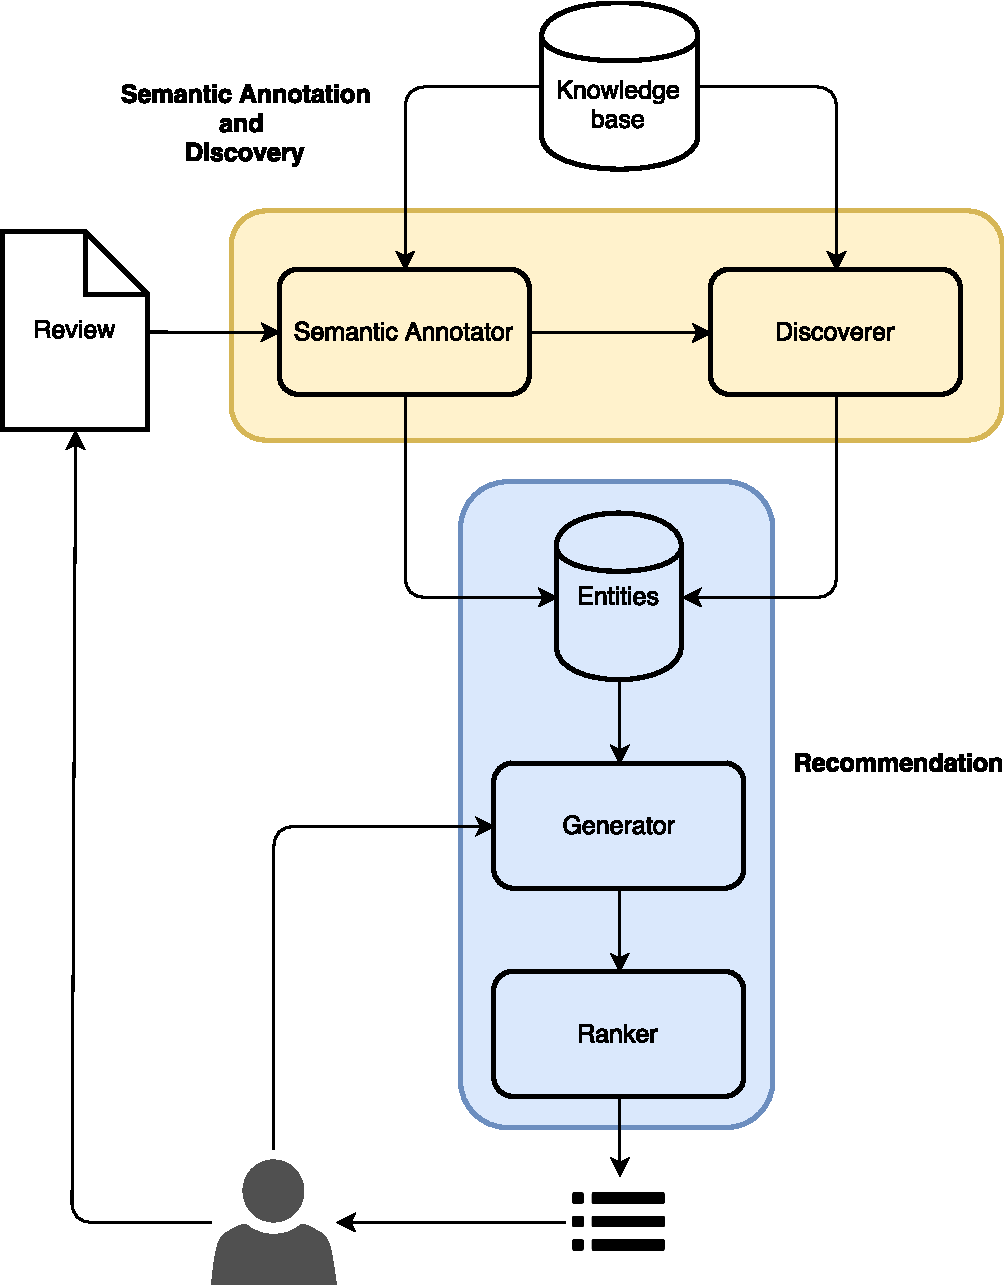
\includegraphics[width=0.65\textwidth]{architecture}
\caption[SemRevRec architecture]{The system architecture of SemRevRec.}
\label{srr:fig:arch}
\end{figure}

\subsection{Semantic Annotation and Discovery}
\label{srr:sec:annotation}

Semantic annotation is the process of annotating textual or multimedia contents with semantic tags to add information about their meaning~\cite{Saathoff2010}. In written text, this can be done by associating a URI to the recognized entities. We considered two popular semantic annotators that rely on Wikipedia: AIDA~\cite{Hoffart2011} and DBpedia Spotlight~\cite{Daiber2013}. They are both capable of disambiguating entities according to the surrounding context: this is useful because users frequently write acronyms and abbreviations. We finally selected AIDA because it is more accurate according to an independent comparison~\cite{Gangemi2013}.

The module of semantic annotation and discovery analyzes the text of the reviews and stores the identified entities in a relational database. The URI of each annotated entity is associated with the URI of the reviewed item and with the occurrence of that entity in all the reviews of that item. In fact, the same entity may appear again in reviews regarding another item. AIDA is capable of identifying and disambiguating entities mentioned in the review considering, by default, the ones available in YAGO.\footnote{\url{http://www.yago-knowledge.org}}

The YAGO resources are mapped with the equivalent ones available in DBpedia exploiting the similar structure of the URIs. For example, \texttt{yago-res:The\_Matrix} corresponds to \texttt{dbr:The\_Matrix} because their URIs where both generated starting from the title of the same Wikipedia article. In contrast, the mapping between DBpedia and Wikidata relies on the \texttt{owl:sameAs} predicate available in DBpedia. If the same entity corresponds to more than one in the other knowledge base, it is ignored in order to avoid probable inconsistencies. The same holds if there is no \texttt{owl:sameAs} property. In principle, it is also possible to perform the semantic annotation phase relying on a custom knowledge base, but AIDA is provided with a precomputed database that includes all the necessary information for annotating using YAGO. In our case, since DBpedia and Wikidata are both well interlinked with YAGO, it was less time consuming computing the mapping rather than the information needed by the annotator.

Finally, the types of each entity are obtained from the target knowledge base, optionally considering only a subset of them (for example, only the DBpedia ontology types, such as \texttt{dbo:Film}). This is done in order to minimize the amount of information retrieved and to reduce the time required for this operation. The types are stored locally because they are not expected to change often and reading them from a database is more efficient than querying the original knowledge base.

Semantic annotation allows SemRevRec to exploit Linked Data for retrieving additional entities. This is possible because the annotated entities are also resources in the Web of Data. Thus, the discoverer can find resources that are related to the annotated entities in order to enable our system to recommend more items. Reviews are a source of non-trivial relations: for example, in a movie recommendation scenario, a user can mention a movie that reminds him the reviewed one because of the colors, the setting, or the atmosphere, and these features are hardly available as Linked Data. At the same time, Linked Data can enrich information coming from users. For instance, they enable the discoverer to obtain other movies in which an actor mentioned in a review played. The discovery can take into account various properties, from more traditional ones, such as the genre, the director, or the actors, to more unexpected ones, such as other movies shot in the same place.

Given the annotated entities, the discoverer retrieves from the knowledge base other relevant entities through SPARQL queries. It relies on some properties that can be configured and depend on the domain and on the dataset considered. The discovery is not bound to a particular knowledge base or domain. On the contrary, this approach is fairly general since it relies only on RDF and SPARQL. In our implementation, we considered DBpedia and Wikidata, and we focused on movie, book, and music recommendations. Table~\ref{srr:tab:disc} summarizes the properties that we selected for discovering further items to recommend starting from the entities available in the reviews.

\begin{table}
\centering
\begin{tabular}{@{}lll@{}}
\toprule
Domain & DBpedia               & Wikidata          \\ \midrule
Movie  & \texttt{dbo:starring} & \texttt{wdt:P161} \\
Movie  & \texttt{dbo:director} & \texttt{wdt:P57}  \\
Book   & \texttt{dbo:author}   & \texttt{wdt:P50}  \\
Music  & \texttt{dbo:artist}   & \texttt{wdt:P175} \\
Music  & \texttt{dbo:writer}   & \texttt{wdt:P676} \\ \bottomrule
\end{tabular}
\caption[Properties for discovery phase]{The properties considered for the discovery phase.}
\label{srr:tab:disc}
\end{table}

More specifically, the discoverer reads the annotated entities stored during the semantic annotation phase. The discoverer is able to obtain all the resources that have the given entities as an object of the selected properties. For example, in the movie domain, we selected \texttt{dbo:starring} and \texttt{dbo:director} in the case of DBpedia because most of the annotated properties, when not movies, were actors and directors. This allows the system to discover other movies from the same director or actor named in a given review. Sometimes directors or actors not involved in the movie were also mentioned for comparison. The discoverer can retrieve other movies from these entities that are relevant for the user who wrote the review, thus can also be of interest for other users. Similarly to movies, we selected \texttt{dbo:author} for books as well as \texttt{dbo:artist} and \texttt{dbo:writer} for music because most of the annotated entities were authors, artists or writers when not books and songs, respectively. It is possible to exploit both direct and inverse properties.
 
The discoverer stores the discovered entities in a relational database for efficiency reasons. The URI of each discovered entity is associated with the URI of the annotated entity through which it was discovered, and, optionally, with the LDSD measure~\cite{Passant2010} between them. This measure is inversely proportional to the number of links between two resources: more links result in a lower distance. Each discovered entity may be found through more than a single annotated entity. The LDSD can be exploited in the ranking phase, which is described in Section~\ref{srr:sec:ranking}. However, since its computation is expensive due to the various SPARQL queries involved, it may be optionally skipped to speed up the discovery step. Obviously, in this case, the LDSD measure does not contribute to the ranking.

\subsection{Recommendation}
\label{srr:sec:recommendation}

The recommendation process consists of two main steps: the generation of the candidate recommendations and their ranking. Given an initial item, SemRevRec retrieves all the entities that are related to the initial item and then ranks them.

Firstly, the system selects the annotated entities that were mentioned in the reviews of the initial item. Afterwards, it obtains the entities that mention the initial item, that is entities whose reviews generated an annotated entity that corresponds to the initial item. For example, if the initial item is \emph{Interstellar} and a review of \emph{2001: A Space Odyssey} mention \emph{Interstellar}, then \emph{2001: A Space Odyssey} is considered as a candidate recommendation.

Secondly, SemRevRec optionally retrieves the discovered entities. They may include entities discovered through the initial item. For instance, if the initial item is \emph{Interstellar} and \emph{The Dark Knight} was previously discovered because both these movies have been directed by Christopher Nolan, \emph{The Dark Knight} is selected. The same holds if \emph{Interstellar} was discovered from \emph{The Dark Knight}, that is Christopher Nolan was annotated in the reviews of the latter. Similarly, the entities discovered through other entities that were annotated in the reviews of the initial item are relevant. For example, if \emph{Interstellar} is the initial item, Stanley Kubrick was annotated in one of its reviews, and \emph{2001: A Space Odyssey} was discovered through Stanley Kubrick, then \emph{2001: A Space Odyssey} is a candidate recommendation.

It is possible to configure the generator to include in the candidate recommendations the discovered entities or not. It is also possible to specify the minimum occurrence required for entities to be included in the candidate recommendation set, which is expressed as a percentage of the maximum occurrence of entities in the reviews of the item considered.

\subsection{Ranking Functions}
\label{srr:sec:ranking}

Finally, SemRevRec ranks the candidate recommendations. We defined three different ranking functions. The first one is presented in Equation~\ref{srr:eq:r1} and takes into account only the occurrence $occur(i)$ of the entities available in the reviews. $occur(i)$ is equal to the number of reviews of an initial item $i_{in}$ where an entity $i$ is annotated plus the number of reviews of $i$ where $i_{in}$ is annotated (if any). However, the entity $i$ can be annotated or discovered. For the latter, the occurrence of the entity through which it was discovered is used. The $\alpha$ coefficient is $1$ if $i$ is an annotated entity. Otherwise, it can be configured to a custom value (the default is $0.5$) to weight the contribution of a discovered entity to the ranking. To obtain a value between $0$ and $1$, R1 is normalized to the maximum occurrence of entities $j$ that belong to the candidate recommendation set $CR$.

\begin{equation}
\label{srr:eq:r1}
\mathit{R1}(i) = \frac{\alpha \cdot \mathit{occur(i, i_{in})}}{max_{j \in \mathit{CR}}(\mathit{occur(j, i_{in})})}
\end{equation}

The second ranking function (Equation~\ref{srr:eq:r2}) also considers the LDSD measure between each discovered entity and the entity through which it was discovered. This avoids assigning the same value to all the entities discovered through the same annotated entity as R1 does. 
As for R1, the entity $i$ can be annotated or discovered. The $\beta$ coefficient is $1$ if $i$ is an annotated entity, $0.5$ otherwise. The $\gamma$ coefficient is $0.5$ for discovered entities, $0$ otherwise. In this way, R2 returns a number between $0$ and $1$, which is equal to R1 for the annotated entities, while, for the discovered entities, it is the average of R1 and $LDSD(i,i_o)$, where $i_o$ is the entity through which $i$ was discovered.

\begin{equation}
\label{srr:eq:r2}
\mathit{R2}(i) = \beta \cdot \mathit{R1}(i) + \gamma \cdot (1 - \mathit{LDSD}(i, i_o))
\end{equation}

The third ranking function (Equation~\ref{srr:eq:r3}) considers the LDSD measure between an entity $i$ and the initial item $i_{in}$. The coefficients $\eta$ and $\kappa$ can be set to custom values and they allow the ranker to weight differently the contribution of the occurrence in the review (given by R2) and Linked Data (through the LDSD).

\begin{equation}
\label{srr:eq:r3}
\mathit{R3}(i) = \eta \cdot \mathit{R2}(i) + \kappa \cdot (1- \mathit{LDSD}(i, i_{in}))
\end{equation}

LDSD measures between discovered entities and the entities through which they were discovered need to be precomputed at discovery time (see Section~\ref{srr:sec:annotation}) to enable SemRevRec to exploit R2, LDSD measures between entities in $CR$ and the initial item need to be computed while ranking.% In the latter case, the ranking time is increased.

\section{Evaluation Procedure}
\label{srr:sec:eval}

We evaluated the performance of SemRevRec with two offline experiments conducted in the movie, book, and music domains. The purpose of the first experiment is to understand the impact of the ranking function, the discovery, the occurrence threshold, and the coefficients of R3. Furthermore, we performed the first experiment two times, first relying on DBpedia and then on Wikidata, to assess the effect of the knowledge base on the quality of the recommended items. The aim of the second experiment is to compare our proposal with traditional recommendation techniques that rely on ratings and a recommender system based on Linked Data.

For conducting both experiments, we obtained from IMDb, LibraryThing, and Amazon the user reviews regarding all the items included in the MovieLens~1M,\footnote{\url{http://grouplens.org/datasets/movielens/1m/}} the LibraryThing\footnote{\url{http://www.macle.nl/tud/LT/}} and the HetRec 2011 LastFM\footnote{\url{http://ir.ii.uam.es/hetrec2011/datasets/lastfm/readme.txt}} datasets of user ratings.

The items of such rating datasets were mapped with the corresponding entities available in DBpedia relying on the work of Di Noia et al.~\cite{DiNoia2016}. Furthermore, their equivalent entities in Wikidata were obtained from DBpedia itself, as described in Section~\ref{srr:sec:annotation}. For the purpose of retrieving the user reviews, Wikidata was exploited in order to discover the IMDb identifiers of the movies available in the MovieLens~1M dataset. On the contrary, the LibraryThing dataset already contained the references useful for obtaining the reviews. Regarding the musical artists present in the HetRec 2011 LastFM dataset, we relied on the search feature of Amazon for identifying their most reviewed musical work.

\begin{table}
\centering
\begin{tabular}{@{}lrrr@{}}
\toprule
                   & Movie     & Book         & Music   \\ \midrule
Users              & 6,040     & 7,279        & 1,892   \\
Items              & 3,706     & 37,232       & 17,632  \\
Ratings            & 1,000,209 & 2,056,487    & 92,834  \\
Reviews            & 559,858   & 363,791      & 669,978 \\
Distinct entities  & 107,468   & 77,120       & 70,762  \\
Total entities     & 574,435   & 303,705      & 296,777 \\ \bottomrule
\end{tabular}
\caption[Statistics about datasets and reviews]{Statistics about the available datasets and reviews.}
\label{srr:tab:stats}
\end{table}

\begin{figure}
\centering
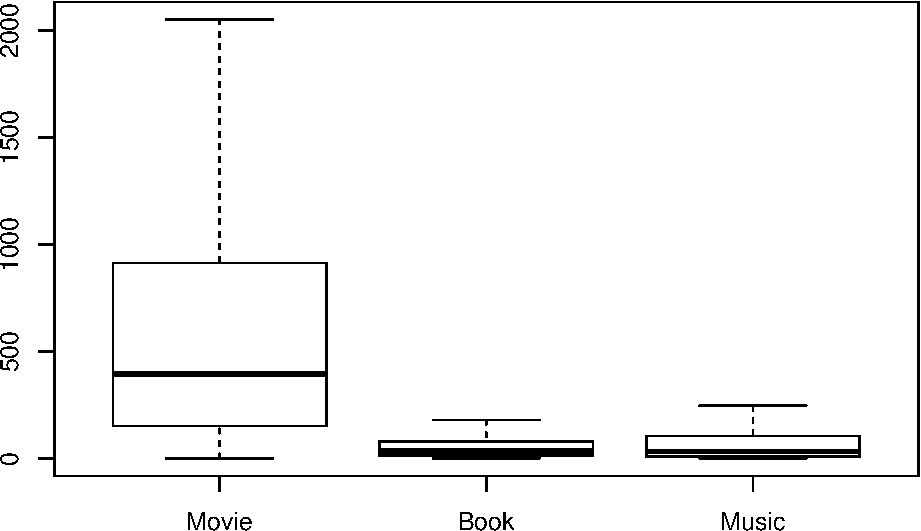
\includegraphics[width=0.85\textwidth]{boxplot}
\caption[Entities extracted from the reviews]{Distribution of entities extracted from the reviews per domain.}
\label{srr:fig:boxplot}
\end{figure}

Table~\ref{srr:tab:stats} lists several statistics regarding the exploited rating datasets and the analyzed reviews in the three domains considered. It is worth noting that the LastFM dataset contains a limited number of ratings with respect to the other datasets and, for this reason, it is the most sparse one. The LibraryThing dataset includes a considerable number of items, even if fewer reviews are available in the book domain. Regarding the outcome of the semantic annotation, the number of distinct and total entities identified in user reviews is reported. The ratio between these two values may be considered a measure of the variety of the mentioned topics. According to this measure, the reviews about movies are the most varied ones in terms of entities.

Figure~\ref{srr:fig:boxplot} displays the boxplots representing the distributions of the number of annotated entities per each item according to the domain, excluding the outliers for graphical reasons. Given the interquartile range $IQR = Q3 - Q1$, all data points not belonging to the interval $(Q1 - 1.5 \cdot IQR; Q3 + 1.5 \cdot IQR)$ are considered outliers. It is clear that movie reviews are fairly different from the other ones. This may be related to the higher ratio between reviews and items in the movie domain.

We relied on a 5-fold cross-validation in order to perform the evaluations. We considered ratings positive if their score was greater than~3 on a scale from 1 to~5 for MovieLens, greater than 6 on a scale from 1 to~10 for LibraryThing, and greater than~0 for LastFM. In fact, the latter dataset contains implicit feedback, while the others are examples of explicit feedback. Exploiting the lists of the top-10 recommendations for each user, we computed the measures of precision, recall, nDCG, Entropy Based Novelty (EBN)~\cite{Bellogin2010}, and diversity~\cite{Zhang2008}.

For the implementation, we rely on the LibRec library.\footnote{\url{https://www.librec.net}} It computes measures according to the \emph{all unrated items} protocol \cite{Steck2013}. More specifically, it creates a top-$k$ recommendation list for each user by predicting a score for every item not rated by that particular user, whether that item appears in the user test set or not. All the non-rated items are considered to be irrelevant for the user. This explains the low values for the measures (in particular precision and recall) as the quality of recommendations tend to be underestimated. However, Steck \cite{Steck2013} suggests to rely on this protocol rather than the \emph{rated test-items}, which includes only rated test items in the top-$k$ list, as the user satisfaction regarding top-$k$ recommendations depends on the ranking of all items.

\section{Evaluation Results}
\label{srr:sec:res}

We report the results of the first experiment on optimizing the parameters of our SemRevRec system in Section~\ref{srr:sec:exp1}. The results of comparing our approach with baselines from related work are documented in Section~\ref{srr:sec:exp2}.

\subsection{Optimizing the SemRevRec Parameters}
\label{srr:sec:exp1}

In this experiment, we evaluated the impact of the ranking function, the discovery, the occurrence threshold, and the coefficients of R3 on the performance of our algorithm. We executed SemRevRec in three domains with different ranking functions with and without the discovery phase. We also varied the configuration parameters $\eta$ and $\kappa$ of the ranking function R3, in order to identify possible relationships between the occurrence and the LDSD measure. Furthermore, we considered how the percentage of the minimum occurrence required for entities to be included in the candidate recommendation set impacts on the results. The main configurations tested are listed in Table~\ref{srr:tab:config}.

\begin{table}
\centering
\begin{tabular}{@{}llllll@{}}
\toprule
Conf. & Ranking & Discovered & Occurrence & $\eta$ & $\kappa$ \\ \midrule
C1    & R1      & False      & 0.05       & --     & --       \\
C2    & R1      & True       & 0.05       & --     & --       \\
C3    & R2      & False      & 0.05       & --     & --       \\
C4    & R2      & True       & 0.05       & --     & --       \\
C5    & R3      & False      & 0.05       & 0.50   & 0.50     \\
C6    & R3      & True       & 0.05       & 0.50   & 0.50     \\
C7    & R3      & True       & 0.05       & 0.75   & 0.25     \\
C8    & R3      & True       & 0.05       & 0.25   & 0.75     \\
\bottomrule 
\end{tabular}
\caption[Configuration parameters of SemRevRec]{The configuration parameters of SemRevRec.}
\label{srr:tab:config}
\end{table}

Table~\ref{srr:tab:ex1-ml}, Table~\ref{srr:tab:ex1-lt}, and Table~\ref{srr:tab:ex1-fm} summarize the results obtained with the DBpedia knowledge base in the movie, book, and music domain. For all the measures but EBN, higher values represent better results, while the lower is EBN, the higher is the novelty. The best values and configurations are highlighted in boldface.\footnote{More values are highlighted for the same measure if the differences among them are not statistically significant.} For deciding if the difference between two measures was statistically significant, we relied on the Welch's \emph{t}-test (or unequal variances \emph{t}-test), an adaptation of the Student's \emph{t}-test more reliable when the two samples have unequal variances and unequal sample sizes~\cite{Ruxton2006}. We considered \emph{p}~<~0.001 because we applied the Bonferroni correction as we performed pairwise comparisons.

The obtained results suggest that the discovery of additional entities through Linked Data is useful for improving the precision of the recommended items. In fact, the best configurations in all the domains but music (C8 for movies, C2 for books) rely on it. In the music domain there is not a significant difference in the measures when relying on the discovery phase. This may be related to the fact that we considered reviews about musical works in order to recommend musical artists.

The best ranking function depends instead on the domain. For movies, R3 outperformed the other rankers (C8), while, for book and music recommendations, R1 accounts for the best results (C2), although in the music domain the values obtained with R1 and R2 were equivalent (C4). This suggests that a simpler ranker may be more effective on sparse data, and it could be better to rely on information from reviews than on Linked Data. Additionally, the coefficients $\eta$ and $\kappa$ of R3 may have a high impact on the results as shown by C6, C7, and C8 in Table~\ref{srr:tab:ex1-ml}, even if, in the music domain, the measures do not vary. In particular, C8 improves significantly the precision and recall measures with respect to other configurations of R3 in the movie and book domains.

\begin{table}
\centering
\begin{tabular}{@{}lrrrrr@{}}
\toprule
Conf.       & Precis.         & Recall          & nDCG            & EBN             & Divers. \\ \midrule
C1          & 0.0604          & 0.0399          & 0.0412          & 1.2804          & \textbf{0.2431} \\
C2          & 0.0529          & 0.0327          & 0.0343          & 1.2776          & 0.1629  \\
C3          & 0.0604          & 0.0399          & 0.0412          & 1.2804          & \textbf{0.2431} \\
C4          & 0.0276          & 0.0178          & 0.0197          & \textbf{0.7820} & 0.1716  \\
C5          & \textbf{0.0683} & 0.0424          & 0.0491          & 1.0047          & 0.1795  \\
C6          & 0.0460          & 0.0255          & 0.0320          & 0.9354          & 0.1794  \\
C7          & 0.0344          & 0.0191          & 0.0243          & 0.8248          & 0.1464  \\
\textbf{C8} & \textbf{0.0711} & \textbf{0.0478} & \textbf{0.0524} & 1.0163          & 0.2114  \\ \bottomrule
\end{tabular}
\caption[Experimental results with MovieLens and DBpedia]{Experimental results obtained with MovieLens and DBpedia.}
\label{srr:tab:ex1-ml}
\end{table}

\begin{table}
\centering
\begin{tabular}{@{}lrrrrr@{}}
\toprule
Conf.       & Precis.         & Recall          & nDCG            & EBN             & Divers. \\ \midrule
C1          & 0.0396          & 0.0350          & 0.0341          & 0.4081          & 0.7701  \\
\textbf{C2} & \textbf{0.0506} & \textbf{0.0497} & \textbf{0.0465} & 0.2771          & 0.7780  \\
C3          & 0.0396          & 0.0350          & 0.0341          & 0.4081          & 0.7701  \\
C4          & 0.0357          & 0.0340          & 0.0353          & \textbf{0.1946} & 0.8919  \\
C5          & 0.0462          & 0.0373          & \textbf{0.0462} & 0.2809          & 0.8663  \\
C6          & 0.0356          & 0.0331          & 0.0366          & 0.2280          & 0.9039  \\
C7          & 0.0306          & 0.0269          & 0.0317          & 0.2444          & 0.8932  \\
C8          & 0.0421          & 0.0418          & \textbf{0.0429} & 0.2077          & \textbf{0.9118} \\ \bottomrule
\end{tabular}
\caption[Experimental results with LibraryThing and DBpedia]{Experimental results obtained with LibraryThing and DBpedia.}
\label{srr:tab:ex1-lt}
\end{table}

\begin{table}
\centering
\begin{tabular}{@{}lrrrrr@{}}
\toprule
Conf.       & Precis.         & Recall          & nDCG            & EBN             & Divers. \\ \midrule
\textbf{C1} & \textbf{0.0495} & \textbf{0.0504} & \textbf{0.0486} & 0.7894          & 0.5654  \\
\textbf{C2} & \textbf{0.0504} & \textbf{0.0515} & \textbf{0.0473} & 0.6640          & 0.6021  \\
\textbf{C3} & \textbf{0.0495} & \textbf{0.0504} & \textbf{0.0486} & 0.7894          & 0.5654  \\
\textbf{C4} & \textbf{0.0504} & \textbf{0.0515} & \textbf{0.0473} & 0.6640          & 0.6022  \\
C5          & 0.0363          & 0.0371          & 0.0378          & 0.2619          & 0.9238  \\
C6          & 0.0360          & 0.0370          & 0.0378          & \textbf{0.2422} & \textbf{0.9325}  \\
C7          & 0.0361          & 0.0369          & 0.0378          & \textbf{0.2425} & \textbf{0.9325}  \\
C8          & 0.0360          & 0.0368          & 0.0378          & \textbf{0.2411} & \textbf{0.9329} \\ \bottomrule
\end{tabular}
\caption[Experimental results with LastFM and DBpedia]{Experimental results obtained with LastFM and DBpedia.}
\label{srr:tab:ex1-fm}
\end{table}

\begin{figure}
\centering
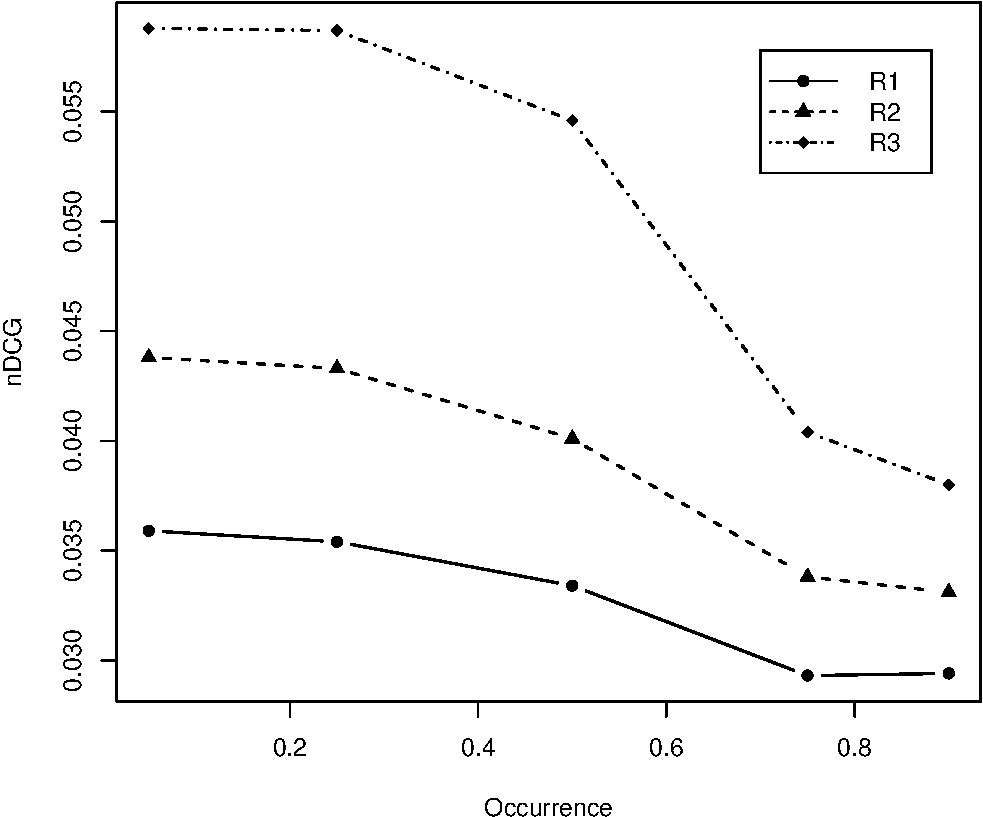
\includegraphics[width=0.75\textwidth]{lineplot}
\caption[nDCG with MovieLens and Wikidata]{The nDCG score obtained by varying the number of entities considered with MovieLens and Wikidata.}
\label{srr:fig:lineplot}
\end{figure}

Figure~\ref{srr:fig:lineplot} illustrates the performance in terms of nDCG of the three ranking functions available in SemRevRec when the number of entities considered for the recommendation process varies. The occurrence represents the minimum number of times an entity needs to be annotated in the reviews of a certain item in order to be included in the candidate recommendation set. It is expressed as a percentage of the most annotated entity for an item. The plot is based on the results obtained in the movie domain with the Wikidata knowledge base, as this can be considered the most representative case. Unsurprisingly, all rankers tend to converge, as the number of entities available decreases. However, it is important to notice that the nDCG is monotonically decreasing. This fact happens in the majority of the domains with both knowledge bases and supports the hypothesis that the higher is the number of available entities, the better is the quality of the recommendations.

\begin{sidewaysfigure}[p]
\centering
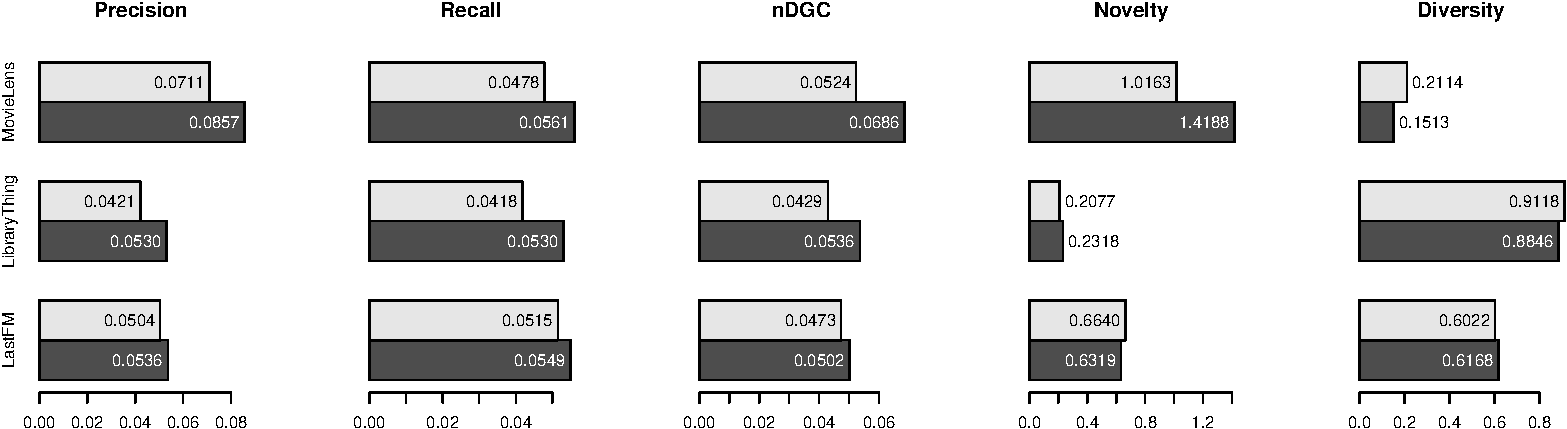
\includegraphics[width=\textwidth]{barplot}
\caption[Comparison between DBpedia and Wikidata]{A comparison between DBpedia and Wikidata. Light grey represents DBpedia, dark grey Wikidata.}
\label{srr:fig:barplot}
\end{sidewaysfigure}

Figure~\ref{srr:fig:barplot} compares the results obtained by the best configuration of our algorithm when using DBpedia and Wikidata for each domain. Although both knowledge bases are derived from Wikipedia, the results differ. In particular, Wikidata outperformed DBpedia in the vast majority of the considered measures. A possible reason may be that Wikidata provides higher data quality for the recommendation task, as it also contains knowledge manually encoded by human editors. At the instance level, this may be primary due to the interlinking of resources since we rely on the LDSD measure that exploits direct and indirect links. At the ontology level, the properties considered in the discovery may also have an high impact. We should investigate which features of a knowledge base are well suited for a Linked Data-based recommender system, although they can also depend on the particular domain considered.

Table~\ref{srr:tab:ex1-wd} lists the results obtained with Wikidata. They vary significantly when the $\eta$ and $\kappa$ weights of the ranking function R3 are changed. Thus, we decided to include in this chapter only the results related to the configurations C4, C6, C7, and C8, although we tested all the ones listed in Table~\ref{srr:tab:config}. The complete evaluation is available on the Web.\footnote{\url{https://doi.org/10.6084/m9.figshare.5074081}} In general, Wikidata provides better results with respect to DBpedia and this behavior is consistent in all domains, but differences are more significant when movies are recommended.

\begin{table}
\centering
\begin{tabular}{@{}llrrrrr@{}}
\toprule
Conf. & Domain  & Precis. & Recall & nDCG   & EBN    & Divers. \\ \midrule
C4    & Movie   & 0.0582  & 0.0368 & 0.0438 & \textbf{1.3626} & 0.1223 \\
C6    & Movie   & 0.0757  & 0.0487 & 0.0588 & 1.4284 & \textbf{0.1461} \\
C7    & Movie   & 0.0728  & 0.0459 & 0.0552 & 1.4322 & \textbf{0.1423} \\
\textbf{C8} & \textbf{Movie} & \textbf{0.0857} & \textbf{0.0561} & \textbf{0.0686} & 1.4188 & \textbf{0.1513} \\
\midrule
C4    & Book   & 0.0392   & 0.0373 & 0.0379 & 0.2634 & 0.8455  \\
C6    & Book   & 0.0452   & 0.0443 & 0.0466 & 0.2621 & 0.8705  \\
C7    & Book   & 0.0365   & 0.0334 & 0.0380 & 0.2809 & 0.8600  \\
\textbf{C8} & \textbf{Book}  & \textbf{0.0530} & \textbf{0.0530} & \textbf{0.0536} & \textbf{0.2318} & \textbf{0.8846} \\
\midrule
\textbf{C4} & \textbf{Music} & \textbf{0.0536} & \textbf{0.0549} & \textbf{0.0502} & 0.6319 & 0.6168 \\
C6    & Music  & 0.0384   & 0.0395 & 0.0375 & \textbf{0.3083} & \textbf{0.9314} \\
C7    & Music  & 0.0390   & 0.0401 & 0.0380 & \textbf{0.3062} & \textbf{0.9327} \\
C8    & Music  & 0.0367   & 0.0377 & 0.0363 & \textbf{0.3178} & \textbf{0.9322} \\ \bottomrule
\end{tabular}
\caption[Experimental results with Wikidata]{Experimental results obtained with Wikidata.}
\label{srr:tab:ex1-wd}
\end{table}

\subsection{Comparison with Baselines}
\label{srr:sec:exp2}

We compared our technique to the Most Popular, Random Guess, Item KNN, and Bayesian Personalized Ranking (BPR)~\cite{Rendle2009} algorithms, as implemented in LibRec, and with SPrank~\cite{DiNoia2016}, a state-of-the-art Linked Data-based recommender. We set the neighborhood size for Item KNN to 80, while we used 100 factors for BPR, as done by Musto et al.~\cite{Musto2016}. We configured SPrank to exploit LambdaMart as the ranking method and to follow in the DBpedia graph the same properties that we selected for our algorithm, as listed in Table~\ref{srr:tab:disc}.

Table~\ref{srr:tab:ex2-ml}, Table~\ref{srr:tab:ex2-lt}, and Table~\ref{srr:tab:ex2-fm} list the results obtained in the movie, book, and music domain, respectively. The best values are highlighted in boldface.\footnote{More values are highlighted for the same measure if the differences among them are not statistically significant. In the case of EBN and diversity, when Random Guess was the best, we also highlighted the second best because its precision, recall, and nDCG were close to zero. This means that the recommendations provided are completely unrelated and their novelty and diversity are not relevant.} For SemRevRec, we reported both the configuration with the best trade-off among the various measures and the best scores achieved for each measure in the experiment described in Section~\ref{srr:sec:exp1}. In all the experimental trails, SemRevRec provided the best diversity and a better accuracy (both in rating prediction and ranking) than SPrank, while it improved in novelty with respect to traditional techniques. BPR accounted for the highest precision, recall, and nDCG. In general, the diversity is rather low for movies, while for music and books is above 0.6, apart for Item KNN.

The differences between SemRevRec and the other approaches are statistically significant according to the Welch's \emph{t}-test with \emph{p}~<~0.001, except for SPrank, BRP, Most Popular, and Random Guess in the movie domain regarding the measure of diversity, SPrank in the book domain regarding the measures of precision and diversity, and Most Popular in the music domain regarding the measure of diversity.

\begin{table}
\centering
\begin{tabular}{@{}lrrrrr@{}}
\toprule
Algorithm & Precis. & Recall & nDCG   & EBN    & Divers. \\ \midrule
SemRevRec & 0.0857  & 0.0561 & 0.0686 & 1.4188 & 0.1513 \\
-- Best Scores & 0.0857 & 0.0561 & 0.0686 & \textbf{0.7820} & \textbf{0.2431} \\ \midrule
SPrank    & 0.0445  & 0.0254 & 0.0280 & 0.8813 & 0.1612 \\
Item KNN  & 0.1626  & 0.1105 & 0.1302 & 2.6846 & 0.0696 \\
BPR       & \textbf{0.2347}  & \textbf{0.1737} & \textbf{0.1930} & 1.8358 & 0.1769 \\
Popular   & 0.1325  & 0.0840 & 0.0969 & 2.7439 & 0.1412 \\
Random    & 0.0055  & 0.0028 & 0.0031 & \textbf{0.3018} & 0.1679 \\ \bottomrule
\end{tabular}
\caption[Comparison using the MovieLens dataset]{Experimental comparison using the MovieLens dataset.}
\label{srr:tab:ex2-ml}
\end{table}

\begin{table}
\centering
\begin{tabular}{@{}lrrrrr@{}}
\toprule
Algorithm & Precis. & Recall & nDCG   & EBN    & Divers. \\ \midrule
SemRevRec & 0.0530  & 0.0530 & 0.0536 & 0.2318 & 0.8846 \\
-- Best Scores & 0.0530  & 0.0530 & 0.0536 & 0.1946 & \textbf{0.9118} \\ \midrule
SPrank    & 0.0379  & 0.0346 & 0.0337 & \textbf{0.1562} & 0.8037 \\
Item KNN  & 0.0620  & 0.0564 & 0.0662 & 1.4956 & 0.2259 \\
BPR       & \textbf{0.0862}  & \textbf{0.0817} & \textbf{0.0895} & 0.6043 & 0.7177 \\
Popular   & 0.0423  & 0.0343 & 0.0447 & 1.6034 & 0.6483 \\
Random    & 0.0004  & 0.0002 & 0.0003 & \textbf{0.0382} & \textbf{0.9879} \\ \bottomrule
\end{tabular}
\caption[Comparison using the LibraryThing dataset]{Experimental comparison using the LibraryThing dataset.}
\label{srr:tab:ex2-lt}
\end{table}

\begin{table}
\centering
\begin{tabular}{@{}lrrrrr@{}}
\toprule
Algorithm & Precis. & Recall & nDCG   & EBN    & Divers. \\ \midrule
SemRevRec & 0.0536  & 0.0549 & 0.0502 & 0.6319 & 0.6168 \\
-- Best Scores & 0.0536  & 0.0549 & 0.0502 & 0.2411 & \textbf{0.9329} \\ \midrule
SPrank    & 0.0156  & 0.0158 & 0.0176 & \textbf{0.1834} & 0.9077 \\
Item KNN  & 0.1392  & 0.1428 & 0.1720 & 1.6023 & 0.4730 \\
BPR       & \textbf{0.1545}  & \textbf{0.1583} & \textbf{0.1808} & 0.9404 & 0.6547 \\
Popular   & 0.0686  & 0.0703 & 0.0791 & 2.0360 & 0.6519 \\
Random    & 0.0005  & 0.0005 & 0.0004 & \textbf{0.0442} & \textbf{0.9946} \\ \bottomrule
\end{tabular}
\caption[Comparison using the LastFM dataset]{Experimental comparison using the LastFM dataset.}
\label{srr:tab:ex2-fm}
\end{table}

\section{Discussion}
\label{srr:sec:discussion}

In general, the results obtained by our algorithm in the music and book domains are not as good as the ones achieved with movie recommendations. This may be due to the characteristics of the reviews, as illustrated in Figure~\ref{srr:fig:boxplot} and previously discussed. The entities annotated for each item in these two domains are much less than the entities available in movie reviews. This fact should be further studied. Furthermore, it would be interesting to investigate the impact of the number of reviews available and their quality with respect to the recommendation process. For example, a meaningful album review mentions the author and similar albums or artists the user liked, while a review describing the package is not very useful in our scenario. In fact, we aim to suggest other artists to listen to, although packaging may impact on the decision of buying a physical copy of that album. Finally, the significant difference in the results obtained when exploiting Wikidata or DBpedia suggests that the impact of knowledge bases, notably the selection of types and properties exploited, on the performance should be further analyzed.

In this work, we relied on all the reviews available for the items present in the rating datasets used for the evaluation. However, only reviews about some items, for example the ones with the average rating higher than a threshold, or only some reviews for each item, for example only the ones that are rated positively, could be considered during the semantic annotation phase. Nevertheless, lower performance on music artists and books was expected because the available ratings were more sparse than the ones regarding movies. This holds for all the algorithms and explains the general difference of scores in these domains. 

SemRevRec showed the best diversity. In the sparse dataset of books, it achieved precision, recall, and nDCG comparable to Item KNN with a much higher diversity, although the former is a content-based method. Collaborative filtering techniques are known to suffer less of the overspecilization problem and provide better rating prediction and ranking than content-based ones. For this reason, although collaborative filtering is very popular, we decided to include in the baseline a technique among many, that is BPR, one of the newest and most promising. Nevertheless, it showed a lower diversity than our algorithm. Not surprisingly, it also accounted for the best rating prediction and ranking. 

Our approach also provided a higher novelty than traditional techniques and a better rating prediction and ranking than SPrank. In the movie domain, SemRevRec accounted for the best novelty, while with music and books for the second best, with results close to SPrank. Additionally, when optimized for this measure, SemRevRec had similar or higher rating prediction and ranking than SPrank. On the contrary, when the former is optimized for rating prediction and ranking, it could be preferred to the latter to increase the novelty of recommendations, while also limiting the loss in rating prediction and ranking.

Finally, SemRevRec was evaluated considering the recommendations generated for all the previous items a user liked, as its generation approach is rather naive and it takes into account only an initial item. Combining it with a machine learning technique could significantly improve its performance, but further experiments are required to prove this.

\section{Conclusion}
\label{srr:sec:concl}

In this chapter we proposed a novel recommendation approach based on the semantic annotation of user reviews and Linked Data. We conducted an offline study of the recommender system in the movie, book, and music domains, which showed that our method provides the best diversity. It also improved rating prediction and ranking compared to another algorithm based on Linked Data, while it increased the novelty of recommendations with respect to traditional techniques. Furthermore, we tested our approach with different knowledge bases and Wikidata systematically achieved better results than DBpedia. Although the reviews available for the book and music domains seem to contain a smaller amount of useful information, the results of the offline study suggest that our algorithm can provide more diverse recommendations and reach an interesting compromise between the accuracy and the novelty of the suggested items.

This work represents a practical application of multicriteria evaluation approaches, but it also raises further interesting research issues that still need to be properly addressed. For this reason, we intend to investigate in greater details how the nature of the user reviews influences the performance of our algorithm. Furthermore, the significant difference in the results obtained when exploiting Wikidata or DBpedia suggests that too little is known about how knowledge bases (notably their types and properties) might impact on the performance of Linked Data-based recommender systems. We also plan to take into account the sentiment of the reviews, that is whether the overall opinion on the item reviewed is positive or negative. Finally, we are evaluating applications of our approach on textual resources different than reviews, for example research papers or their abstracts. In this case sentiment would not be relevant, while annotated entities could be concepts representing the main topics addressed in the document.

\chapter{Second Use Case: Music Recommender System}
\graphicspath{{Chapter09/Figures/}}
\label{chap:challenge}

In recent years, music streaming services strongly modified the way in which people access to music content. In particular, the music experience does not foresee anymore to follow pre-defined collections of tracks edited by music artists or labels: the end-user is now free to produce her own playlist with potentially unlimited freedom. As a consequence, the automatic playlist generation and continuation are now crucial tasks in the recommender system field.

This chapter describes the results obtained by the D2KLab team, lead by the author of this dissertation, for the task of playlist completion obtained in the context of the RecSys Challenge 2018. This work relies on an ensemble strategy which involves different types of features, including sequential embeddings, title embeddings and lyrics features. Therefore, the proposed approach could be considered a multicriteria sequence-based recommender system. Following the challenge rules,\footnote{\url{https://recsys-challenge.spotify.com/rules}} the target dataset is the Million Playlist Dataset (MPD), which contains metadata for 1 million playlists gathering more than 2.2 million distinct tracks. The implementation of our approach is publicly available on GitHub.\footnote{\url{https://github.com/D2KLab/recsys18_challenge}}

The remainder of this chapter is structured as follows: Section~\ref{rnn:sec:ensemble} presents our ensemble approach, while Section~\ref{rnn:sec:rnn} details the design of the Recurrent Neural Networks. In Section~\ref{rnn:sec:t2r} we discuss the intuition behind the implementation of Title2Rec. Section~\ref{rnn:sec:optimization} explains the optimization conducted on the ensemble, the RNN, and Title2Rec. We describe the experimental results in Section~\ref{rnn:sec:results}. Finally, in Section~\ref{rnn:sec:conclusion}, we provide the conclusions.

\section{Ensemble}
\label{rnn:sec:ensemble}

Our approach builds upon an ensemble voting strategy of different runs of multiple Recurrent Neural Networks (RNNs) and one execution of Title2Rec. The RNNs are configured differently in terms of network inputs and hyper-parameters. The RNNs are used to predict the missing tracks to be part of a playlist and thus assume to have seed(s) track(s) of the playlist to be utilized as initial elements of the network bootstrap (Section~\ref{rnn:sec:rnn}). However, when only the title of the playlist is available, our approach relies on a fall-back strategy that implements a K-means clustering of the playlists and a word embedding model of their titles (trained with fastText), called Title2Rec (Section~\ref{rnn:sec:t2r}). Figure~\ref{rnn:fig:ensemble} illustrates the overall approach.

\begin{figure}
\centering
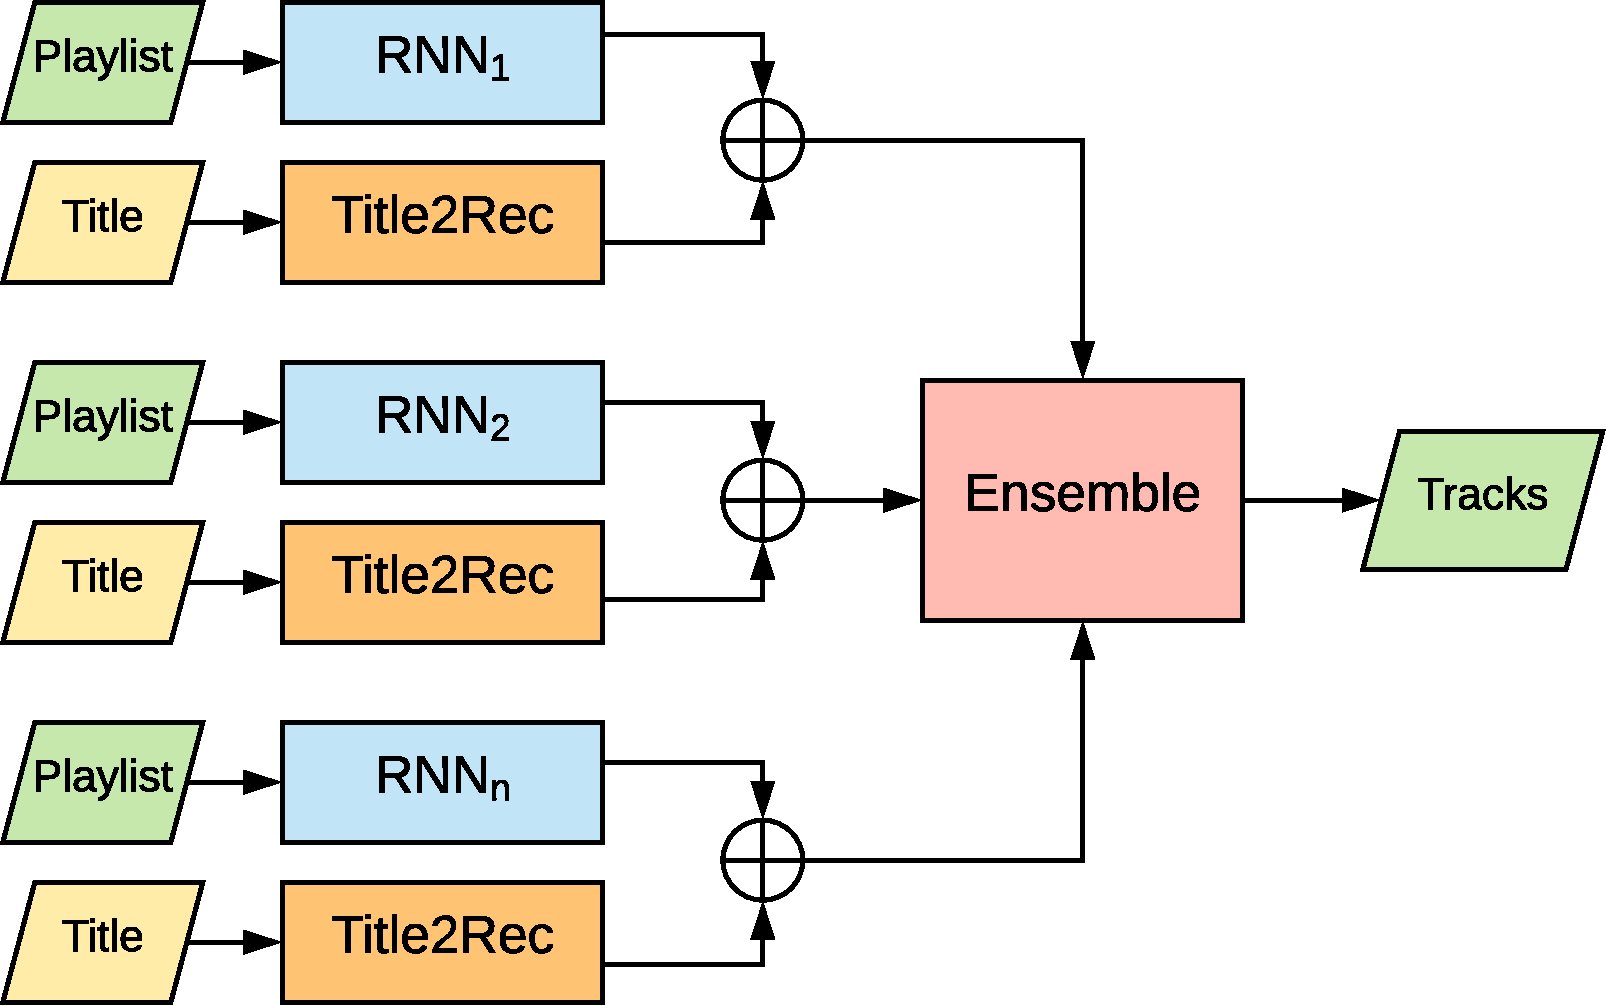
\includegraphics[width=\textwidth, width=0.75\textwidth]{ensemble}
\caption[Ensemble architecture for playlist completion]{The proposed ensemble architecture for playlist completion. The inputs are a playlist and its title.}
\label{rnn:fig:ensemble}
\end{figure}

The ensemble weighs the rankings of the different runs by giving more importance (more weights) to the top ranked tracks and less to the low ranked tracks, similarly to a Borda count election. In detail, given a ranked set of predictions coming from a configuration $k$, corresponding to a particular configuration of the RNN jointly combined with Title2Rec, $R_k = \{T_1, T_2, \dots, T_{500}\}$, we assign to each track a score $s_k$ that has its maximum for the first track in the ranking and minimum for the last one, i.e. $s_k(T_i) = 500 - i + 1$. Then, we sum the scores over all the configurations that we want to ensemble, obtaining a final score for each track $s(T_i) = \sum_{k} s_k(T_i)$ that we use to create the final ranking of the tracks. Take as an example (with 3 tracks instead of 500 in the predictions) a configuration $1$ with ranking $R_1 = \{T_1, T_2, T_3\}$ and a configuration $2$ with ranking $R_2 = \{T_1, T_3, T_2\}$. We would get $s_1(T_1) =  3$, $s_1(T_2) = 2$, $s_1(T_3) = 1$, $s_2(T_1)=3$, $s_2(T_3) = 2$, $s_2(T_2)=1$ and thus $s(T_1) = 3+3= 6$, $s(T_2)= 2+1=3$, $s(T_3)=1+2=3$, obtaining as a final ranking $R = \{T_1, T_2, T_3\}$, or equivalently $R = \{T_1, T_3, T_2\}$ as $T_2$ and $T_3$ have the same score.

\section{Recurrent Neural Networks}
\label{rnn:sec:rnn}

Recurrent Neural Networks (RNNs) are one of the most commonly used typology of neural networks~\cite{Lecun2015}. In recent years, thanks to advancements in their architecture~\cite{Hochreiter1997,Chung2014} and in computational power, they have become the standard to effectively model sequential data. They have been used successfully for tasks such as sentiment analysis~\cite{Tang2015}, speech recognition~\cite{Graves2013}, image captioning~\cite{Karpathy2015}, predicting tourist paths~\cite{Palumbo2017} and neural language models~\cite{Mikolov2010}. One of the typical applications of RNNs is language modeling, i.e. the task of learning a probabilistic model of text in order to generate new text by recursively predicting the next word in a sentence~\cite{Sutskever2011}. We use RNNs, more specifically Long-Short Term Memory (LSTM) cells~\cite{Hochreiter1997}, in a similar vein to the language modeling problem, i.e. training the network to predict the next track in a playlist and sampling tracks from the learned probability model to generate predictions. In practice, rather than using only the track as input, we use a richer representation that also exploits the artist, the album, the title and, possibly, lyrics features (Figure~\ref{rnn:fig:global_architecture}). 

In the following sections, we describe in detail the input features as well as the generation strategy.

\begin{figure}
\centering
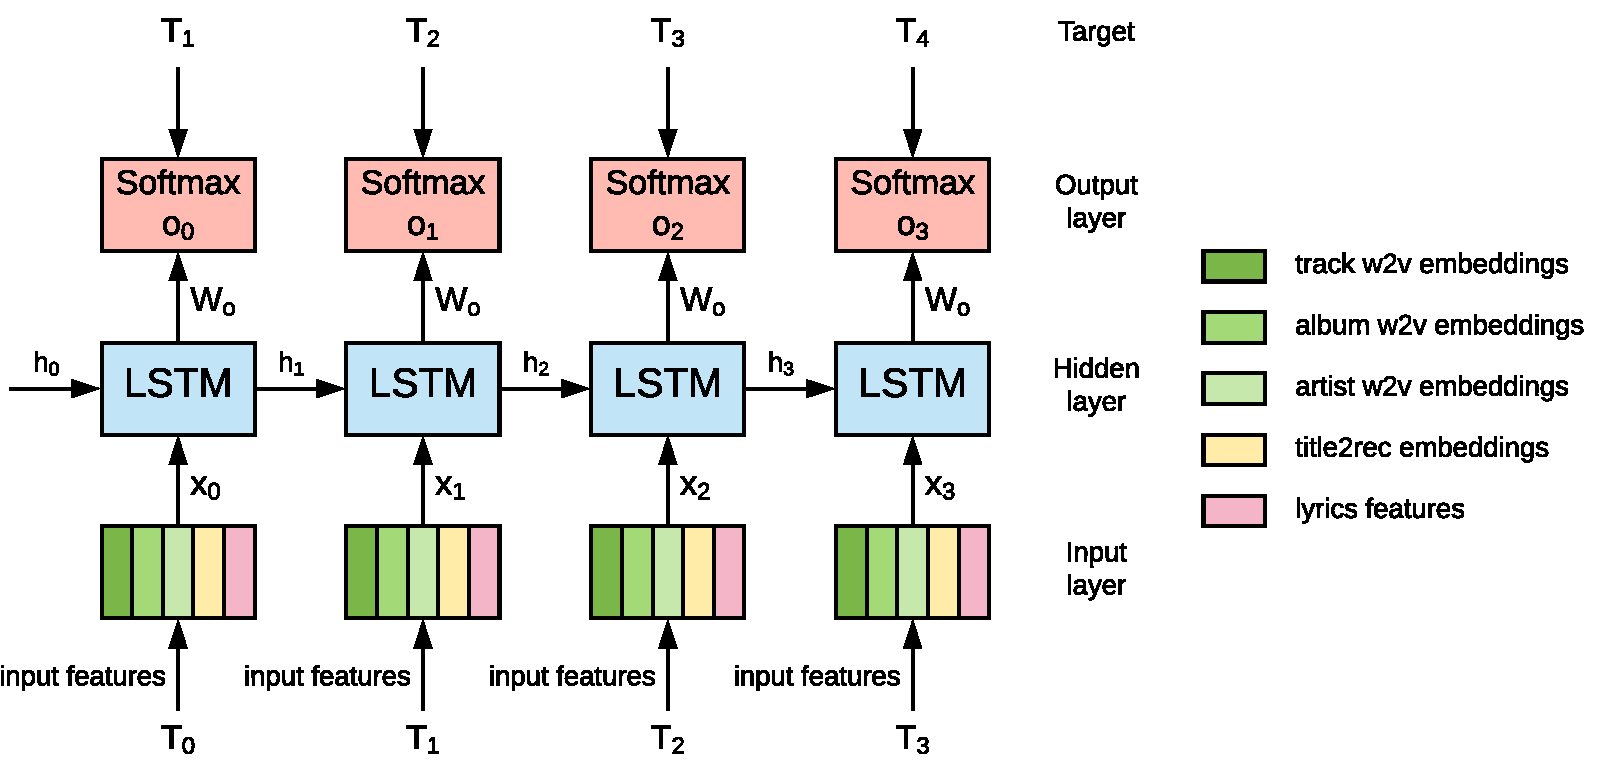
\includegraphics[width=\textwidth]{rnn}
\caption[RNN architecture for playlist completion]{Our RNN architecture for playlist completion. The input vectors include word2vec embeddings for the track, the album, and the artist, a fastText embedding for the playlist title and numerous features extracted from the lyrics.}
\label{rnn:fig:global_architecture}
\end{figure}

\subsection{Input Vectors}

\subsubsection{Track, Album and Artist Embeddings}
\label{rnn:sec:track_embs}

In order to leverage the information in the dataset concerning tracks, artists and albums, we opt for an approach based on word2vec~\cite{Mikolov2013} embeddings. More precisely, we train the word2vec model separately on sequences of tracks, albums and artists in the order of appearance in the playlist, obtaining three separated word2vec models encoding co-occurrence patterns of tracks, albums and artists respectively. Each word2vec model is based on the Skip-gram model with negative sampling using default hyper-parameters of the Gensim implementation~\cite{Rehurek2010}: embedding vector dimension is $d=100$, learning rate $\alpha = 0.025$ linearly decaying up to $min_{\alpha} = 0.0001$, window size $c = 5$, number of epochs is $\eta = 5$.

We concatenate the three representations of the tracks, albums and artists, obtaining an input vector $x_{w2v}$ whose dimensionality is $|x_{w2v}| = 300$.

\subsubsection{Title Embeddings}
\label{rnn:sec:title_embs}

The title of a playlist can potentially contain interesting information about the intention and the purpose of its creator. The title can suggest that the tracks in certain playlist are intended to suit a certain goal (e.g. \textit{party}, \textit{workout}), a mood (\textit{sad songs}, \textit{relaxing}), a genre (\textit{country}, \textit{reggae}), or a topic (\textit{90's}, \textit{Christmas}). Our intuition, supported by the experiments described later in this section, is that playlists with similar titles may contain similar tracks.
The title similarity could rely on pre-trained models and thesauri. However, we opted for computing a model that is specific for the playlist continuation task, using the sole data of the MPD.

A playlist embedding $p_{w2v}$ is computed as the mean of the embeddings of the tracks composing the playlist, as generated in the previous section. The playlist embeddings are then grouped in $n$ clusters, applying the K-means algorithm~\cite{Hartigan1979}.

We empirically observed that, apart from very general clusters, we also created clusters containing specialized playlists, obtaining as a consequence groups of titles that belong to the same semantic area. For example, a cluster contains playlists like \textit{Christmas feels}, \textit{December} or with titles including the emoji of Santa Claus, while another group encompasses playlists like \textit{country} and \textit{Alabama}.

Each cluster $c$ expresses a composed label, which is the concatenation of the titles of all the playlist $p \in c$ separated by a blank space. These labels can be seen as a corpus of $n$ documents (one for each cluster) that is used as input for the fastText algorithm~\cite{Joulin2016}. Because this algorithm is able to represent textual information at the level of n-grams from 3 to 6 character, the Title2Rec model in output computes the embeddings of any playlist title, being this already seen in the dataset or totally unknown. Figure~\ref{rnn:fig:t2r_pipeline} illustrates the process of the Title2Rec model generation.

\begin{figure}
\centering
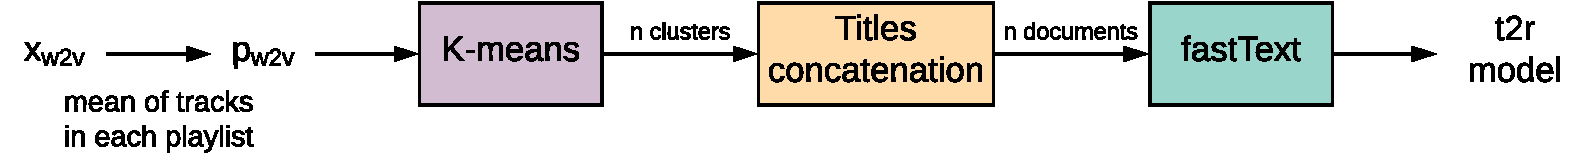
\includegraphics[width=\textwidth]{t2r}
\caption[Pipeline for the title embedding model]{The pipeline for generating the title embedding model used in Title2Rec. The embeddings are computed through a fastText model trained on a corpus of concatenated titles of similar playlists.}
\label{rnn:fig:t2r_pipeline}
\end{figure}

\subsubsection{Lyrics Embeddings}
\label{rnn:sec:lyrics}

Since playlists contain tracks that share semantic properties (such as the genre) and acoustic properties (such as the mood), we hypothesize their lyrics share features as well. To this end, we extract numerous features from the lyrics for a large set of tracks used in the MPD dataset ($v \in \mathbb{R}^{n}$) that describe different stylistic and linguistic dimensions of a song text:

\begin{itemize}
\item \textit{vocabulary} ($v \in \mathbb{R}$): as a measure of the vocabulary richness, we compute the type-token ratio of a song text.
\item \textit{style} ($v \in \mathbb{R}^{27}$): to estimate the linguistic style of a song text, we measure the line lengths (in characters and in tokens) and the frequencies of all major part-of-speech tags. We further count rhyme occurrences and \qu{echoisms} (sung words like \qu{laaalala} and \qu{yeeeeeeeaaaaaaah}).
\item \textit{semantics} ($v \in \mathbb{R}^{60}$): we build a topic model with 60 topics on the song text bag of words using Latent Dirichlet Allocation~\cite{Blei2003}. Each song text is then represented by its association to these topics.
\item \textit{orientation} ($v \in \mathbb{R}^{3}$): this dimension models how the song narrative (entities, events) is oriented with respect to the world. We encode a temporal dimension, i.e. whether the song mainly recounts past experiences or present/future ones, by representing the fraction of past tense verb forms to all verb forms as a feature.
\item \textit{emotion} ($v \in \mathbb{R}^{6}$): we model the subjectivity (subjective vs. objective) as well as the polarity (positive vs. negative) of the song text. Furthermore, the emotions conveyed are modelled in a common two-dimensional model that accounts for degrees of arousal and valence.
\item \textit{song structure} ($v \in \mathbb{R}^{4}$): as a proxy of the structure of the lyrics, we use the line lengths as well as the lengths of paragraphs in the song text.
\end{itemize}

For experimental purposes, we grouped the previous features in two categories:

\begin{itemize}
\item \textit{deterministic} ($v \in \mathbb{R}^{23}$): it encompasses all features generated in a deterministic way such as features related to the structure, the vocabulary, and the style of the lyrics. We excluded from this group the frequencies of part-of-speech tags, as they depend on the tagger used.
\item \textit{fuzzy} ($v \in \mathbb{R}^{18}$): it includes the features generated in a non-deterministic fashion such as orientation, emotion, and the frequencies of POS tags.
\end{itemize}

All features are scaled using a custom feature scaler that combines two elements. It accounts for outliers by scaling the data non-linearly based on the percentile of the feature value distribution they belong to. Finally, it scales the data linearly to the same $[-1,1]$ interval that non-lyrics features live in.

Retrieving lyrics for the MPD dataset is achieved by linking it to the WASABI corpus~\cite{Meseguer2017}.\footnote{\url{https://wasabi.i3s.unice.fr}} The WASABI corpus is an ongoing resource that contains 2.1M song texts (of 77k artists), and for each song it provides the following information: the lyrics extracted from \url{http://lyrics.wikia.com}, the synchronized lyrics (when available) from \url{http://usdb.animux.de}, DBpedia abstracts and categories the song belongs to, genre, label, writer, release date, awards, producers, artist and/or band members, the stereo audio track from Deezer (when available), the unmixed audio tracks of the song, its ISRC, BPM, and duration. In total, we linked 416k tracks in MPD (out of 2.2M unique tracks) to WASABI tracks that contain the lyrics. While the linked tracks proportion with $\sim$20\% seems small, the linked tracks cover 53\% of all 66M track occurrences in MPD because of the typical fat-tailed distribution, where some songs are extremely common while most titles occur only rarely in a playlist. Linking the lyrics was done in three levels of accuracy: direct Spotify URI matching gave us 155k links, exact artist and title matching provided 334k matches, and finally lower casing and deleting bracketed content (in song titles only) led to 51k matches. As the results overlap we ended up with 416k matched tracks in total. Some of our lyrics features are language-specific, so we decided to compute lyrics features exclusively on English song texts. This finally resulted in 367k English song texts we computed lyrical features on. Language detection is done with the \textit{langdetect} package\footnote{\url{https://github.com/Mimino666/langdetect}} and datasets of MPD and WASABI are merged along the axes of their Spotify URIs, artist names, song title names, respectively.

\subsection{Learning Model}

As mentioned earlier, we address the problem of playlist continuation as a language modeling problem. More specifically, we train the RNN to predict the next track in a playlist, defining the targets $Y$ to be the inputs $X$ shifted in time, i.e. $X = \{(\hat{T{^j}}_0, \hat{T{^j}}_1, \dots, \hat{T^{j}}_{N_j -1})\}$ and $Y = \{(T{^j}_1, T{^j}_2, \dots, T^{j}_{N_j})\}$ where $\hat{T}$ represents a track and its metadata (artist, album, playlist title, lyrics features), $T$ represents a track id in a playlist, $j = 1, \dots, M$ is a playlist index and $N_j$ is the length of the j-\textit{th} playlist. In this way, we train the model to learn a probability distribution of the next track $P (T_N | \hat{T}_{N-1}, \hat{T}_{N-2}, \dots, \hat{T}_{0})$ given the previous ones, which is parametrized by the network outputs that are converted into probabilities by the final softmax layer (Figure~\ref{rnn:fig:global_architecture}). The training algorithm attempts to minimize the cross-entropy loss function $L$, that measures the disagreement between the learned probability model and the observed probability model of the targets $Y$. The perplexity metric that is reported in the experiments is similar to the one detailed in Section~\ref{seq:sec:perplexity} and it corresponds to $ppl = 2^{L}$. In practice, rather than using probabilities, we use the `logits' $p_i$ where $i$ is a track index, un-normalized scores that are proportional to the probabilities. Different optimization algorithms to minimize the loss are empirically compared to select the most appropriate one.

\subsection{Generating Predictions}
\label{rnn:sec:generation}

We experiment three different strategies to generate track predictions from the RNN. Given an input seed and the hidden state, the trained model outputs the logits $p_i$, i.e. un-normalized scores that are proportional to the probability that a given track appears after the sequence of seeds $s$. In details, we considered the following approaches, as depicted in Figure~\ref{rnn:fig:predictions}.

\begin{description}
\item[do\_sample] It samples the track with the highest logit $p_i$, where $\hat{i} = arg\ max ({p_i})$, given the set of seeds $s$. It adds the sampled track $\hat{i}$ to the seeds $s$, then it repeats the previous operations until 500 tracks are sampled.
\item[do\_rank] It ranks the tracks according to their logit value $p_i$, given all the seeds $s$, then it selects the top-500 tracks with the highest logit.
\item[do\_summed\_rank] It computes the logits $p_i$ for every seed. It averages all the logits in the sequence obtaining $\hat{p_i}$ and then it ranks the tracks according to the values of $\hat{p_i}$.
\end{description}

\begin{figure}
\centering
\begin{subfigure}{.8\textwidth}
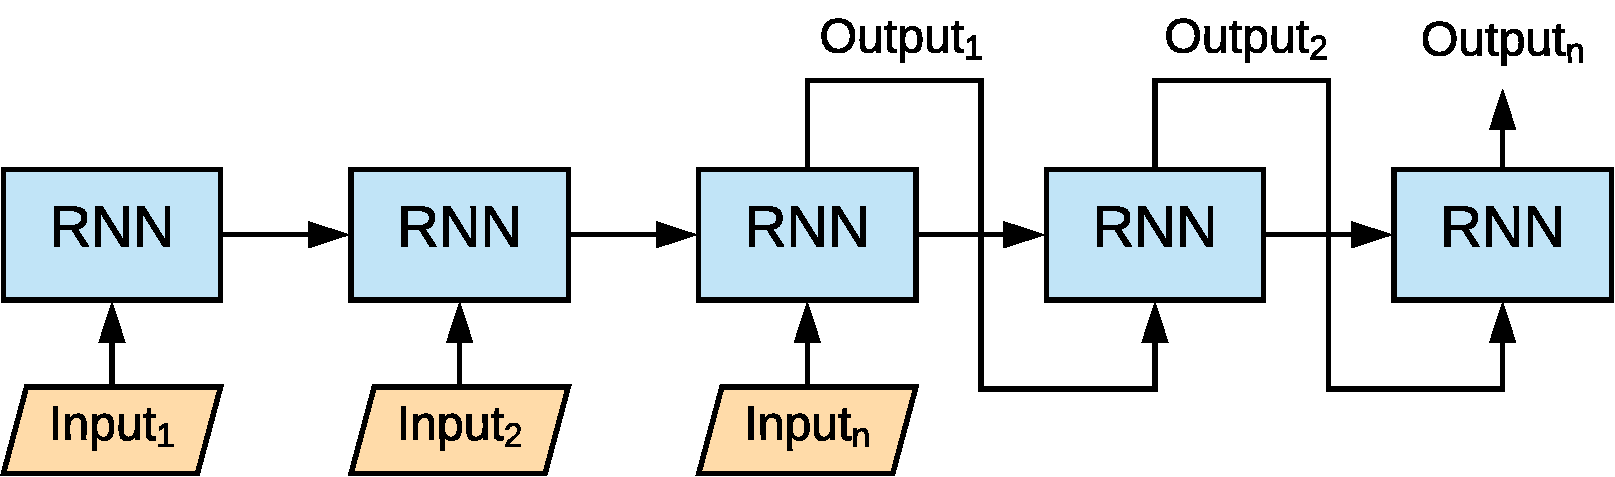
\includegraphics[width=\textwidth]{sample}
\caption{do\_sample}
\bigskip
\end{subfigure}
\begin{subfigure}{.8\textwidth}
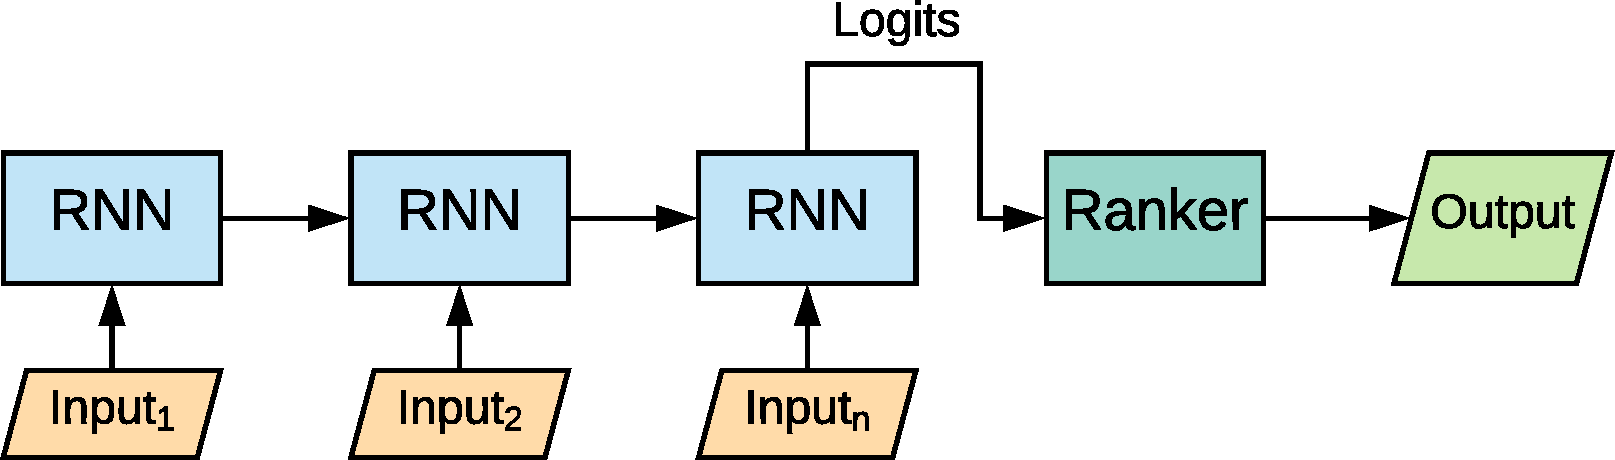
\includegraphics[width=\textwidth]{rank}
\caption{do\_rank}
\bigskip
\end{subfigure}
\begin{subfigure}{.8\textwidth}
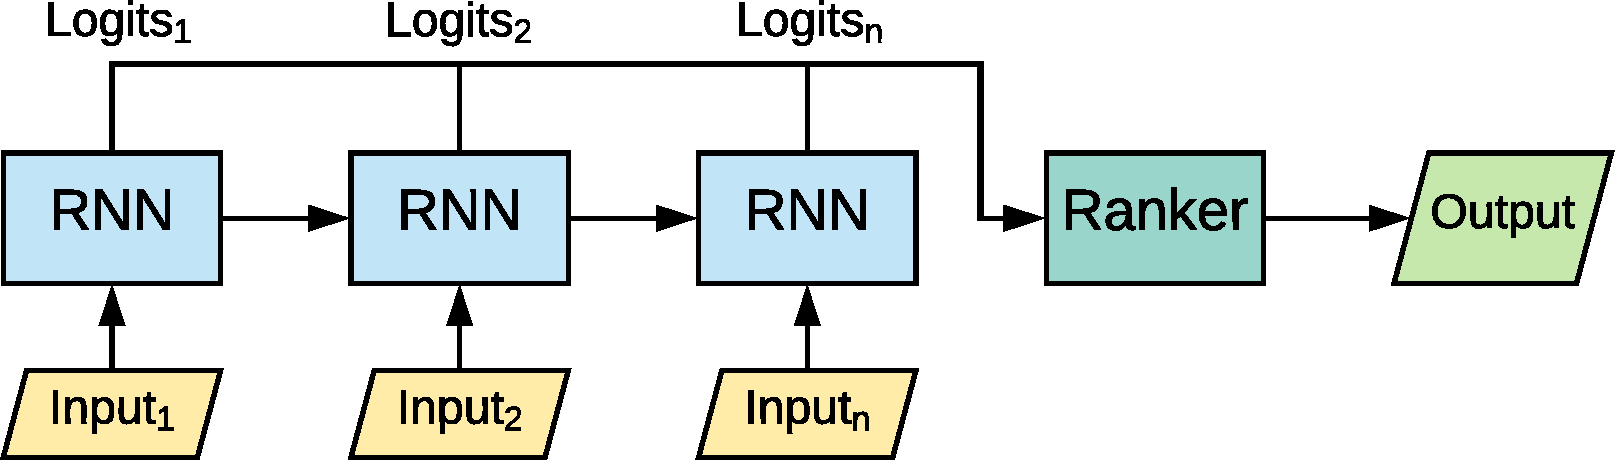
\includegraphics[width=\textwidth]{summed}
\caption{do\_summed\_rank}
\end{subfigure}
\caption[Strategies for generating track predictions]{Our three strategies for generating track predictions.}
\label{rnn:fig:predictions}
\end{figure}

\section{Title2Rec}
\label{rnn:sec:t2r}

Title2Rec recommends tracks taking as input the playlist title, following the procedure illustrated in Figure~\ref{rnn:fig:t2r_rec}. The title is translated into a vector $p_{t2r}$, named title embedding, computed by applying the strategy described in Section~\ref{rnn:sec:title_embs} to the playlists defined in the MPD dataset.

Given a new seed playlist, we compute its title embedding in the same way. Then, we select a subset $P$ including the top-300 most similar playlists to the given one by comparing its embeddings with $p_{t2r}$ using the cosine similarity. Finally, the required number of tracks are selected among the ones available in $P$. The tracks have been ordered to ensure that the most popular ones in $P$ are placed at the top of the list.

\begin{figure}
\centering
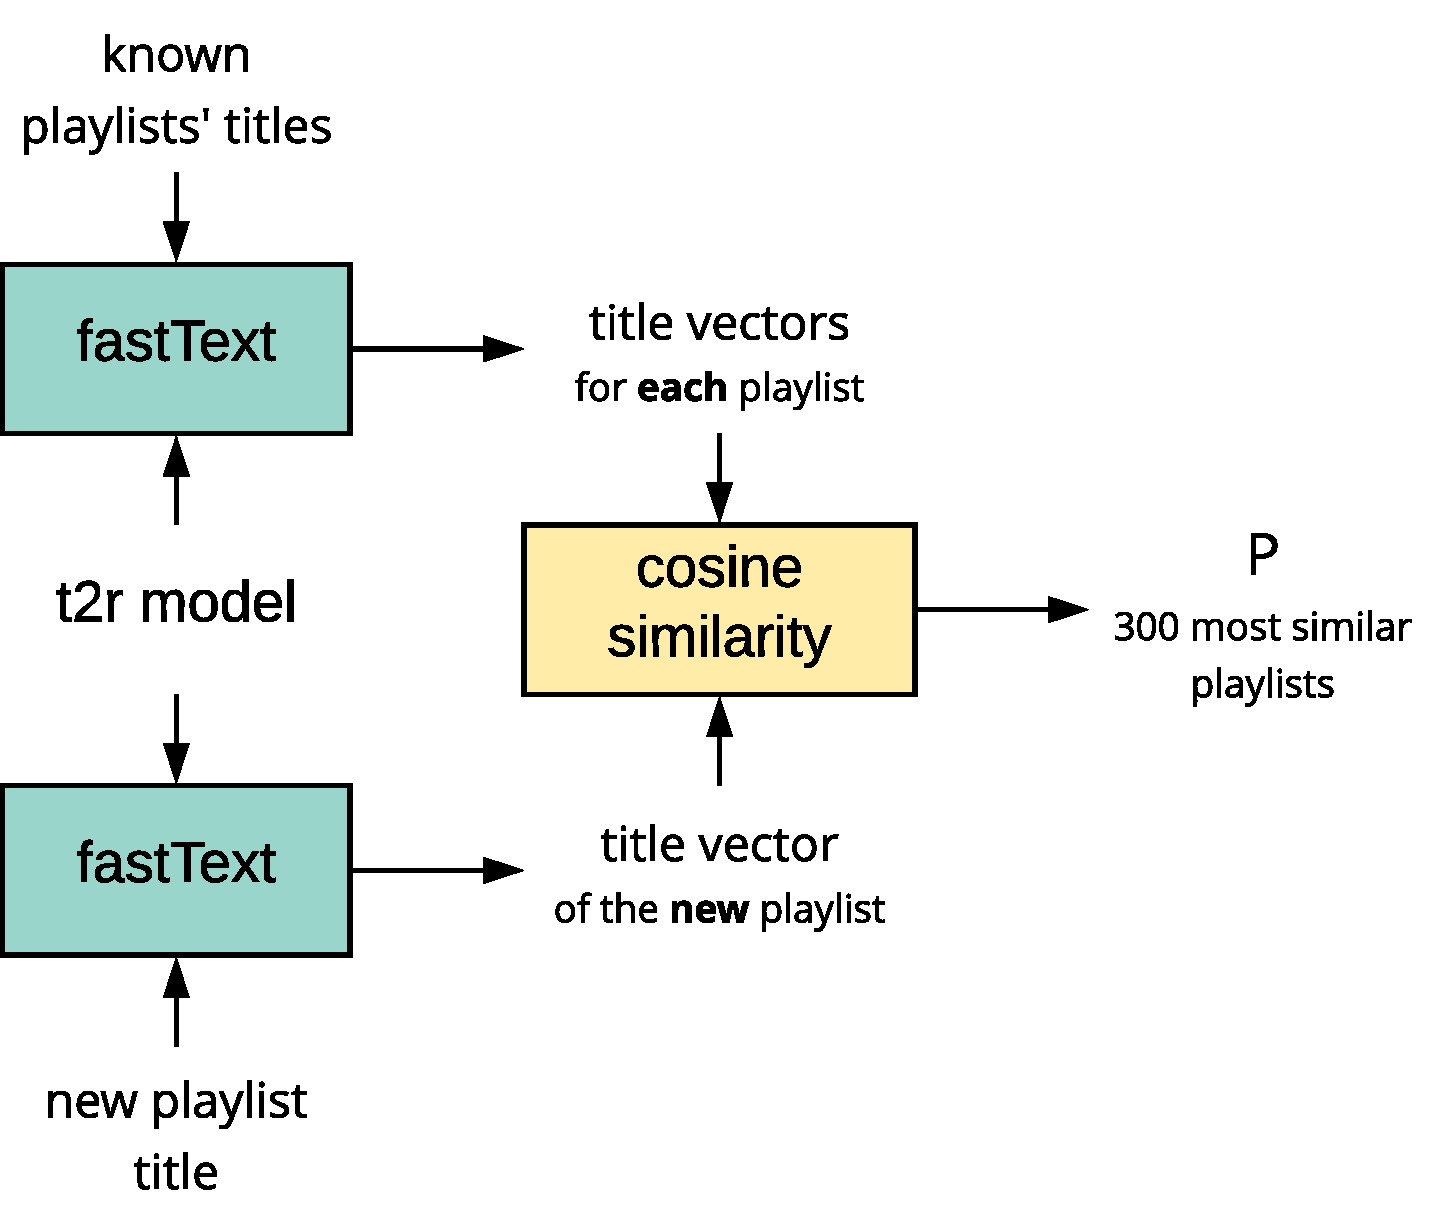
\includegraphics[width=.75\textwidth]{t2r_rec}
\caption[Title2Rec algorithm]{The Title2Rec algorithm compares the fastText representation of the title of a seed playlist to the known ones using the cosine similarity.}
\label{rnn:fig:t2r_rec}
\end{figure}

\section{Optimization}
\label{rnn:sec:optimization}

In the following, we describe the empirical evaluations conducted with the purpose of optimizing the configuration of the RNN, Title2Rec, and the ensemble.

\subsection{RNN Optimization}
\label{rnn:sec:rnn-opt}

For optimizing the hyper-parameters of the RNN, we executed a grid search on a down-sampled version of the MPD dataset containing 100,000 playlists. We considered the following parameters:

\begin{itemize}
\item optimizer: $opt = \{Gradient,\ RMSProp,\ ADAM\}$
\item learning rate: $lr = \{1,\ 0.5,\ 0.1,\ 0.01\}$
\item number of steps: $ns = \{10,\ 20\}$
\item hidden layer size: $hl = \{50,\ 100\}$ 
\end{itemize}

For each configuration $(opt,\ lr,\ ns,\ hl)$, we trained the RNN model and we measured its perplexity on a validation set consisting of 1,000 playlists. Furthermore, we measured its R-Precision, nDCG, and Click metrics as defined in the challenge rules on a separate test set of the same size. The validation and test sets used for optimization purposes contain playlists with the first 5 tracks available as the initial seed, while the others are hidden.

We considered a total of 48 possible configurations: the values of perplexity of the most significant ones are reported in Table~\ref{rnn:tab:rnn_opt}. Perplexity measures the `surprise' of the probabilistic model in observing the data and it is defined as $s^{L}$ where $L$ is the cross-entropy loss function. Thus, lower values of perplexity corresponds to better models. We observe that, when the hidden size is fixed, the best performing optimizer is ADAM. Furthermore, increasing the number of steps reduces the perplexity of the RNN, but it does not have a significant effect on the R-Prec.

Finally, because of time constrains, we selected the configuration $(ADAM,\allowbreak\ 1,\allowbreak\ 10,\allowbreak\ 50)$ as the optimal one, despite its higher perplexity: in fact, we empirically observed that a smaller hidden size results in a shorter training duration.

\begin{table}
\centering
\begin{tabular}{@{}lllllll@{}}
\toprule
Optimizer & L.R. & Steps & Hidden  & ppl     & Time & R-Prec. \\ \midrule
ADAM      & 1    & 20    & 100     & 1357.04 & 3:29 & 0.1739  \\
ADAM      & 1    & 10    & 100     & 1482.86 & 3:39 & 0.1742  \\
Gradient  & 1    & 10    & 100     & 1693.96 & 3:32 & 0.1566  \\
ADAM      & 1    & 10    & 50      & 1716.92 & 2:30 & 0.1745  \\
Gradient  & 1    & 10    & 50      & 2005.54 & 2:25 & 0.1543  \\ \bottomrule
\end{tabular}
\caption[Results of the RNN models]{The results of the most significant RNN models. `L.R.' stands for learning rate, `Steps' for the number of time steps, `Hidden' for the size of the hidden layer, `ppl' stands for perplexity, `Time' is the training time in hours:minutes.}
\label{rnn:tab:rnn_opt}
\end{table}

We evaluated in a controlled setting all the strategies for generating the recommended tracks described in Section~\ref{rnn:sec:generation}. We observed that, independently from other hyper-parameters, the technique called \textit{do\_summed\_rank} systematically achieved better results than the other ones in all the metrics considered. For this reason, we selected this algorithm as our track generation strategy.

Finally, we analyzed the effects on the evaluation metrics of the different categories of features extracted from the lyrics as defined in Section~\ref{rnn:sec:lyrics}, and we selected the groups emotion and fuzzy as the most performing ones.

\subsection{Title2Rec Optimization}
In order to improve the performances of Title2Rec, we worked on different parts of the pipeline. Each optimization has been tested by running the algorithm on a validation set of 1,000 playlists. Then, only the edits that improved the scores with respect to the non-optimized version have been kept in the final version.

We applied a pre-processing on each single title that performed a series of tasks:

\begin{itemize}
\item lowercasing;
\item detecting and separating emoji from words;
\item separating the skin code from the emoji;
\item detecting and separating emoticons from words;
\item transforming space-separated single letters into words (e.g. ``\textit{w o r k o u t}'' becomes ``\textit{workout}'';
\item remove `\#' from hashtags.
\end{itemize}

Other tasks that have been tested with no improvements are:

\begin{itemize}
\item detecting and separating punctuation from words;
\item removing stop words;
\item removing all spaces.
\end{itemize}

The latter point has been partially exploited because we noticed an improvement in the results by including in the corpus both versions of the title, that is keeping the spaces (as in ``green day'') and removing them (``greenday'').

Another optimization step included the usage of different parameters for executing the pipeline. The clustering phase have been tested with different values of $k$ (the number of clusters in output for the K-means algorithm). The value of 500 gives better results than smaller and bigger ones, which produce clusters that are respectively less specialized and less populated. The fastText training has been run with 5 epochs, a learning rate of 0.1 and different loss functions (ns, hs, \textit{softmax}), window sizes (3, \textit{5}, 10). The values in italics represent the best results.

The ordering by popularity described in Section~\ref{rnn:sec:t2r} has been modified so that the impact of each playlist is proportional to the similarity of its title to the seed. In other words, a track has a higher chance to be recommended if it is included in a large number of playlists in $P$ and if most of them are among the top ones more similar to the seed.

Finally, some improvements come from the inclusion of the playlist descriptions in the training. On the whole set of descriptions in the MPD dataset, we compute a TF-IDF model. Thanks to this, we are able to extract a set of keywords for each description by selecting the three words with the highest score. These keywords are added to the documents used to build the clusters. The contribution of the description is null when the playlist does not include any.

\subsection{Ensemble Optimization}

We studied the performance of the ensemble by applying a combination without repetition sampling of different runs for each of the tracks, namely main and creative, and for different groups of runs. In detail, given $n$ the total number of runs, and $k$ the grouping factor, we devised a number of $\frac{n!}{k!(n-k!)}$, where we varied $k=1,\dots,n-1$. We then selected the best performing configuration for both the main and the creative tracks by optimizing the three metrics used for the final ranking. These configurations are reported in Section~\ref{rnn:sec:results}.

\section{Experimental Results}
\label{rnn:sec:results}

In order to evaluate the effectiveness of our approach, we have divided the official MPD dataset in a training, a validation, and a test set. The validation and the test set contain 10,000 playlists each, that is the 1\% of the original dataset. These playlists have been selected according to the characteristics of the MPD provided by Spotify.\footnote{\url{https://recsys-challenge.spotify.com/challenge_readme}} Thus, the validation and test playlists are divided into 10 different categories: each of them defines a peculiar way of hiding some information during the testing phase, i.e. the number of seed tracks or their order.

Furthermore, we have implemented an evaluation tool that computes on our split the same metrics that are described in the challenge rules. Following this approach, it is possible to inspect the evaluation results for each category of the test set separately. As expected, the category containing playlists with only their title and no tracks proved to be the most difficult one to address.

Table~\ref{rnn:tab:approaches} contains the results obtained on our test set by Title2Rec, Word2Rec, and the RNNs trained with different optimizers and input vectors. Word2Rec corresponds to the word2vec model trained on sequences of tracks as described in Section~\ref{rnn:sec:track_embs} and used to generate predictions directly by looking up the 500 most similar tracks to the seeds. All the neural models, but the first two, were trained with the optimal configuration described in Section~\ref{rnn:sec:rnn-opt}. These models are computationally demanding: the training phase lasted more than three days per epoch. The numbers 300 and 400 represent the dimensionality of the input vectors: the 300 models were trained without the title embeddings, while the 400 ones also exploit the fastText model described in Section~\ref{rnn:sec:title_embs}. All the RNNs that include the features extracted from the lyrics were trained with input vectors of dimensionality higher than 400.

\begin{table}
\centering
\begin{tabular}{@{}llllll@{}}
\toprule
Approach    & Optimizer & Epoch & R-Prec.     & nDCG   & Click   \\ \midrule
Title2Rec   & -         & -     & 0.0837      & 0.1260 & 12.007  \\
Word2Rec    & -         & -     & 0.0963      & 0.1444 & 8.4322  \\
RNN 300     & Gradient  & 1     & 0.1417      & 0.1621 & 4.1902  \\
RNN 300     & Gradient  & 2     & 0.1500      & 0.1656 & 3.9433  \\
RNN 300     & ADAM      & 1     & 0.1557      & 0.1702 & 3.9213  \\
RNN 300     & ADAM      & 2     & 0.1457      & 0.1672 & 4.4224  \\
RNN 400     & ADAM      & 1     & 0.1572      & 0.1708 & 3.9340  \\
RNN 400     & ADAM      & 2     & 0.1520      & 0.1694 & 4.1307  \\
RNN Emotion & ADAM      & 1     & 0.1556      & 0.1702 & 4.0101  \\
RNN Emotion & ADAM      & 2     & 0.1500      & 0.1680 & 4.3594  \\
RNN Fuzzy   & ADAM      & 1     & 0.1555      & 0.1698 & 3.9950  \\
RNN Fuzzy   & ADAM      & 2     & 0.1503      & 0.1683 & 4.3456  \\ \bottomrule
\end{tabular}
\caption[Results of different approaches]{Experimental results of different approaches on our test set.}
\label{rnn:tab:approaches}
\end{table}

Table~\ref{rnn:tab:ensemble} lists the results computed on our test set for the best performing configurations in the two tracks of the challenge. The models combined in the ensemble are the following:

\begin{description}
\item[Main track] RNN 300 (Gradient; Epoch 1 and 2), RNN 300 (ADAM; Epoch~1 and 2), and RNN 400 (Epoch 1 and 2).
\item[Creative track] RNN 300 (Gradient; Epoch 1 and 2), RNN 300 (ADAM; Epoch~1 only), RNN 400 (Epoch 1 and 2), RNN Emotion (Epoch 1 and 2), and RNN Fuzzy (Epoch 1 and 2).
\end{description}

\begin{table}
\centering
\begin{tabular}{@{}llll@{}}
\toprule
Track    & R-Precision & nDCG   & Click  \\ \midrule
Main     & 0.1611      & 0.1710 & 3.6349 \\
Creative & 0.1634      & 0.1717 & 3.5964 \\ \bottomrule
\end{tabular}
\caption[Results of the ensemble]{Experimental results of the ensemble on our test set.}
\label{rnn:tab:ensemble}
\end{table}

\section{Conclusion}
\label{rnn:sec:conclusion}

Completing automatically playlists with tracks contained in the MPD dataset is a particularly difficult task due to the dataset dimension and the variety of playlists generated by numerous users having different likes and behaviors bringing great diversity. In this chapter, we presented the D2KLab recommender system that implements an ensemble approach of multiple learning models differently optimized combined with a Borda count strategy. Each model runs an RNN that exploits a wide range of playlist features such as artist, album, track, lyrics (used for the creative track), title and a so-called Title2Rec that takes as input the title and that is used, as fall-back strategy, when playlists do not contain any track. The approach showed to be robust in such a complex setting demonstrating the effectiveness of learning models for automatic playlist completion.

The experimental analysis brought to further attention three points, namely the generation strategy, complementarity of the learning models, and computing time. The generation strategy has a great impact on the results and it pointed out that a recurrent decoding stage is less performing than using a ranking strategy that weighs the output of each RNN of the encoding stage. The ensemble strategy aggregates different outputs of the learning model runs by pivoting the generated ranking. This has granted a sensible increment in performance, so we plan to study further the complementarity of the runs and to build a learning model to automatically select the best candidates. Finally, the computing time has been a crucial experimental setup element due to the generation of the RNN learning model; we addressed it by creating different sizes of the MPD dataset randomly selected and by optimizing the learning models on the hardware at disposal, becoming another factor of differentiation for shaping a performing submission.

\chapter{Conclusion and Future Work}
\label{chap:conclusion}

This dissertation explored different challenges related to the offline evaluation of sequence-based and top-$k$ recommender systems. We proposed to adopt a multicriteria approach to mitigate the popularity bias introduced by many rating datasets and a robust evaluation protocol to ensure the reproducibility of the results. In~particular, we considered three main research lines: identifying the most appropriate metrics to evaluate a sequence-based recommender system, creating a protocol suitable for comparing ranked lists of suggestions, and analyzing the structure of rating datasets to understand their impact on the results of an offline trail.

We proposed two evaluation protocols by formalizing their theoretical backgrounds and by also developing their software implementations. While relying on them, we studied a possible technique to visualize the internal structure of any rating dataset and we designed a method for generating synthetic collections of user preferences that could be successfully exploited to conduct offline evaluations. Finally, we applied our knowledge of multicriteria approaches to different use cases, by designing novel recommendation algorithms and assessing their performance.

In detail, the main contributions of this dissertation are the following:

\begin{itemize}
\item A systematic literature review about multicriteria recommender systems, that was reported in Chapter~\ref{chap:multicriteria}.
\item Sequeval, an offline evaluation protocol for sequence-based recommenders, introduced in Chapter~\ref{chap:sequeval}.
\item A distributed approach to assess the quality of top-$k$ lists of suggestions, called RecLab and discussed in Chapter~\ref{chap:reclab}.
\item RS-viz, a method for visualizing with a 3D scatter plot the ratings available in a dataset, that was presented in Chapter~\ref{chap:rs-viz}.
\item A clustering technique capable of generating synthetic datasets in a realistic way starting from already existing ones, as shown in Chapter~\ref{chap:synthetic}.
\item The evaluation of a recommender based on the entities mentioned in the reviews of the suggested items, described in Chapter~\ref{chap:semrevrec}.
\item The creation of an RNN-based algorithm to suggest sequences of songs to be added to a playlist, that was outlined in Chapter~\ref{chap:challenge}.
\end{itemize}

The systematic literature review explored the topic of multicriteria recommenders, as defined by the structure of their users' preferences. We investigated the approaches currently available in literature and how they were evaluated, considering the protocols, the metrics, and the datasets. We discovered that it is not possible to directly compare different algorithms due to the variability in the evaluation methods adopted by the reviewed studies. Furthermore, the lack of publicly available rating datasets emerged as another critical point.

Sequeval is an experimental protocol for performing the offline evaluation of sequence-based recommender systems. It exploits a multicriteria approach to analyze the suggested sequences from different angles, considering eight metrics. Therefore, the experimenter can select the most promising techniques according to the dimensions she considers the most relevant in a domain of interest. We conducted different experimental campaigns by relying on this framework and we observed that the results are adequate to identify the straights and weaknesses of the recommendation algorithms under investigation.

A similar multifaceted set of metrics was exploited for creating RecLab, a method to evaluate top-$k$ recommender systems in a distributed fashion. By relying on widespread Web protocols, it is possible to assess in a reliable way different algorithms without exposing their implementation details. Please note that both frameworks are not bound to any particular rating dataset or splitting strategy. We empirically observed the effect of the configuration parameters of RecLab on the experimental results considering different domains and recommenders.

To better interpret the results of an evaluation campaign, we proposed and prototyped RS-viz, an interactive visualization method for understanding the structure of the preferences available in a dataset. From the resulting plots, it is possible to intuitively observe unexpected statistical distributions, and, thus, being aware of the probable presence of an associated bias in the suggested items. We validated this hypothesis considering different versions of the LastFM dataset and the numerical results obtained from them with multiple recommenders.

Because of the scarcity of publicly available collections of ratings highlighted by our systematic literature review, we designed a method to generate synthetic datasets that exhibit the same properties of existing ones. By relying on RecLab, we verified that this approach is useful to anonymize potentially private ratings while preserving the possibility of using them to successfully train a recommender system. In particular, we observed that the experimental results obtained when relying on the generated datasets are consistent with the ones of the reference datasets.

We applied a multicriteria evaluation protocol to a recommender system based on the semantic annotation of user reviews, named SemRevRec. The motivating idea of this content-based approach is that users could explicitly mention items that are unexpected but also related with the initial one. Our offline study conducted in multiple domains showed that this method provides the best diversity among the considered approaches, while also increasing the precision of the suggestions with respect to another method based on Linked Data.

Finally, in the context of the RecSys Challenge 2018, we designed a novel sequence-based recommender system based on Recurrent Neural Networks and text embeddings. The goal of this approach is to suggest how to complete a music playlist starting from a few seed songs and the title of the playlist. The proposed method was evaluated in a multicriteria fashion considering three metrics that were defined by the organizers of the challenge. Despite the high competitiveness of this field, our approach has been ranked in the first third of the leaderboard.

The complete list of the publications describing the studies discussed in this dissertation is available in Appendix~\ref{chap:publications}.

\section{Limitations}

In the systematic literature review reported in Chapter~\ref{chap:multicriteria}, we considered as multicriteria only the recommender systems that are capable of exploiting a dataset containing multiple ratings for each user--item pair, thus representing more complex user preferences. This strict choice was necessary to clearly define the scope of our investigation. Nevertheless, in the remainder of this dissertation we focused our attention on the experimental approaches for assessing existing algorithms and we mainly considered ``multicriteria'' as an evaluation technique based on multiple measures. Furthermore, the recommender discussed in Chapter~\ref{chap:challenge} could be considered a multicriteria one with respect to the content-based attributes of the items.

Both Sequeval and RecLab rely on several recommendation performance objectives. However, the availability of many metrics may produce results which are difficult to interpret, especially if we are uncertain of what are the most relevant dimensions in our recommendation scenario. For this reason, it would be useful to define a way for summarizing the outcome of an evaluation campaign. More in general, this is a common limitation of offline experiments, and it needs to be addressed by analyzing the most promising algorithms in a subsequent online trail.

Our visualization toolkit RS-viz was empirically validated by comparing the plots obtained from alternative versions of a rating dataset with the corresponding results of two offline trails involving multiple algorithms. However, we should confirm these results by conducting a user study to investigate if researchers and practitioners are able to correctly use it to explain the performance of different recommender systems in a particular domain.

The approach proposed to generate synthetic datasets starting from an existing one is based on the K-means clustering algorithm. Even if we studied the impact of the value of $K$ on the recommendation results, additional work is required to better understand what is the optimal value for a certain domain. Furthermore, we should also investigate what is the effect of artificially increasing the number of users during the generation phase.

\section{Future work}

The offline comparison of different recommender systems is a challenging task that can be successfully completed only by understating the structure of the rating dataset, the impact of the evaluation protocol, and the meaning of the exploited metrics. Even if in an industrial setting the ultimate method for assessing a recommendation algorithm is studying its impact on company profits, there is anyway the need of conducting offline experiments for comparing a large number of alternatives or selecting the most promising configuration parameters.

This dissertation discussed an evaluation framework for sequence-based recommender systems, a distributed approach for analyzing top-$k$ ranked lists of suggestions, a method for visualizing datasets of user preferences, and a generative approach for creating synthetic ratings. Nevertheless, the outcomes of these studies pose further research challenges that should be address by future works.

Regarding both evaluation toolkits, we plan to study in more depth what are the relationships among the different metrics included in the frameworks, with the purpose of integrating them in a final value that expresses the overall quality of the recommender. Such a global score should be related to the recommendation scenario: for example, diversity may be important when recommending POIs to a tourist, but less useful in the music domain.

Furthermore, it would be desirable to be able to create evaluation frameworks that are adopted by a community of researchers when testing their algorithms, harmonizing the evaluation protocols and the interpretation of the performance of the analyzed recommender systems. For this reason, it is necessary to identify and to include in them some additional meaningful datasets, related to different domains that could be exploited during the evaluation phase, as well as other baselines and novel recommendation methods.

Finally, we would like to expand our evaluation frameworks to also support the online experimentation that should be performed after the offline analysis. The final goal of this dissertation is, in fact, to enable researchers to spend more time in realizing the recommendation algorithm as they can rely on an evaluation protocol that has already been designed and validated.

With respect to RS-viz, we would like to quantitatively characterize rating datasets according to different dimensions and place them in various categories, for example by analyzing the diversity of user preferences or the tendency to rate popular items only. This empirical categorization would enable the users of our tool to better understand the ratings available and to select the most appropriate recommendation approach according to such proprieties.

Furthermore, we would like to improve RS-viz by developing other visualization methods to enable more comprehensive analysis. Finally, additional studies are needed to better understand how the proposed approach could be extended for also visualizing non-conventional datasets, for example the ones enhanced with context-aware information like spatial and temporal data.

Finally, there is the need of exploring additional methods for creating synthetic datasets. We believe that Generative Adversarial Networks (GANs) could be successfully exploited for this task, as they are already used to generate fake images starting from real ones~\cite{Goodfellow2014}. Such approaches would require the definition of a way for representing the preferences of a user similarly to an image.


\appendix
\cleardoublepage
\begin{landscape}
\chapter{Systematic Literature Review}
\label{chap:studies-slr}

\footnotesize
\setlength{\tabulinesep}{3pt}
\begin{longtabu} to \linewidth {l>{\raggedright}X>{\raggedright}Xl>{\raggedright}X>{\raggedright}X}
\toprule
Code & Author & Title & Year & Publication & Source \\ \midrule
\endhead
\bottomrule
\endfoot
\paper{slr:Liu2011} & Liu, L.; Mehandjiev, N.; Xu, D.-L. & Multi-criteria service recommendation based on user criteria preferences & 2011 & Fifth ACM Conference on Recommender Systems & ACM Digital Library \\
\paper{slr:Shambour2011} & Shambour, Q.; Lu, J. & A hybrid multi-criteria semantic-enhanced collaborative filtering approach for personalized recommendations & 2011 & International Conferences on Web Intelligence and Intelligent Agent Technology & ACM Digital Library \\
\paper{slr:Jannach2012} & Jannach, D.; Karakaya, Z.; Gedikli, F. & Accuracy improvements for multi-criteria recommender systems & 2012 & 13th ACM Conference on Electronic Commerce & ACM Digital Library \\
\paper{slr:Hdioud2013} & Hdioud, F.; Frikh, B.; Ouhbi, B. & Multi-criteria recommender systems based on multi-attribute decision making & 2013 & International Conference on Information Integration and Web-based Applications \& Services & ACM Digital Library \\
\paper{slr:Choudhary2017} & Choudhary, P.; Kant, V.; Dwivedi, P. & A particle swarm optimization approach to multi criteria recommender system utilizing effective similarity measures & 2017 & 9th International Conference on Machine Learning and Computing & ACM Digital Library \\
\paper{slr:Musto2017} & Musto, C.; de Gemmis, M.; Semeraro, G.; Lops, P. & A multi-criteria recommender system exploiting aspect-based sentiment analysis of users' reviews & 2017 & Eleventh ACM Conference on Recommender Systems & ACM Digital Library \\
\paper{slr:Park2017} & Park, Y. & Recommending personalized tips on new courses for guiding course selection & 2017 & South-East Conference & ACM Digital Library \\
\paper{slr:Sreepada2017} & Sreepada, R. S.; Patra, B. K.; Hernando, A. & Multi-criteria recommendations through preference learning & 2017 & Fourth ACM IKDD Conferences on Data Sciences & ACM Digital Library \\
\paper{slr:Zheng2017} & Zheng, Y. & Criteria chains: A novel multi-criteria recommendation approach & 2017 & 22nd International Conference on Intelligent User Interfaces & ACM Digital Library \\
\paper{slr:Tallapally2018} & Tallapally, D.; Sreepada, R. S.; Patra, B. K.; Babu, K. S. & User preference learning in multi-criteria recommendations using stacked auto encoders & 2018 & 12th ACM Conference on Recommender Systems & ACM Digital Library \\
\paper{slr:Zheng2018} & Zheng, Y.; Dave, T.; Mishra, N.; Kumar, H. & Fairness in reciprocal recommendations & 2018 & 26th Conference on User Modeling, Adaptation and Personalization & ACM Digital Library \\
\paper{slr:Niknafs2008} & Niknafs, A.; Charkari, N. M.; Niknafs, A. A. & PROMETHEE-based recommender system for multi-sort recommendations in on-line stores & 2008 & Third International Conference on Digital Information Management & IEEE Xplore \\
\paper{slr:Hwang2010} & Hwang, C.-S.; Kao, Y.-C.; Yu, P. & Integrating multiple linear regression and multicriteria collaborative filtering for better recommendation & 2010 & International Conference on Computational Aspects of Social Networks & IEEE Xplore \\
\paper{slr:Liu2010} & Liu, L.; Lecue, F.; Mehandjiev, N.; Xu, L. & Using context similarity for service recommendation & 2010 & IEEE Fourth International Conference on Semantic Computing & IEEE Xplore \\
\paper{slr:Shambour2010} & Shambour, Q.; Lu, J. & A framework of hybrid recommendation system for government-to-business personalized e-services & 2010 & Seventh International Conference on Information Technology: New Generations & IEEE Xplore \\
\paper{slr:Zarrinkalam2012} & Zarrinkalam, F.; Kahani, M. & A multi-criteria hybrid citation recommendation system based on linked data & 2012 & 2nd International eConference on Computer and Knowledge Engineering & IEEE Xplore \\
\paper{slr:Boulkrinat2013} & Boulkrinat, S.; Hadjali, A.; Mokhtari, A. & Enhancing recommender systems prediction through qualitative preference relations & 2013 & 11th International Symposium on Programming and Systems & IEEE Xplore \\
\paper{slr:Samatthiyadikun2013} & Samatthiyadikun, P.; Takasu, A.; Maneeroj, S. & Bayesian model for a multicriteria recommender system with support vector regression & 2013 & IEEE 14th International Conference on Information Reuse \& Integration & IEEE Xplore \\
\paper{slr:Bokde2015} & Bokde, D. K.; Girase, S.; Mukhopadhyay, D. & An approach to a university recommendation by multi-criteria collaborative filtering and dimensionality reduction techniques & 2015 & IEEE International Symposium on Nanoelectronic and Information Systems & IEEE Xplore \\
\paper{slr:Sharma2015} & Sharma, Y.; Bhatt, J.; Magon, R. & A multi-criteria review-based hotel recommendation system & 2015 & IEEE International Conference on Computer and Information Technology; Ubiquitous Computing and Communications; Dependable, Autonomic and Secure Computing; Pervasive Intelligence and Computing & IEEE Xplore \\
\paper{slr:Asawarangsee2016} & Asawarangsee, T.; Maneeroj, S. & A novel aggregation technique for multi-criteria recommendation & 2016 & 13th International Joint Conference on Computer Science and Software Engineering & IEEE Xplore \\
\paper{slr:Ashley-Dejo2016} & Ashley-Dejo, E.; Ngwira, S. M.; Zuva, T. & A context-aware proactive recommender system for tourist & 2016 & International Conference on Advances in Computing and Communication Engineering & IEEE Xplore \\
\paper{slr:Hassan2016} & Hassan, M.; Hamada, M. & Enhancing learning objects recommendation using multi-criteria recommender systems & 2016 & IEEE International Conference on Teaching, Assessment, and Learning for Engineering & IEEE Xplore \\
\paper{slr:Wijayanto2016} & Wijayanto, A.; Winarko, E. & Implementation of multi-criteria collaborative filtering on cluster using Apache Spark & 2016 & 2nd International Conference on Science and Technology-Computer & IEEE Xplore \\
\paper{slr:Hamada2018} & Hamada, M.; Odu, N. B.; Hassan, M. & A fuzzy-based approach for modelling preferences of users in multi-criteria recommender systems & 2018 & IEEE 12th International Symposium on Embedded Multicore/Many-core Systems-on-Chip & IEEE Xplore \\
\paper{slr:Mohamed2018} & Mohamed, H.; Abdulsalam, L.; Mohammed, H. & Adaptive genetic algorithm for improving prediction accuracy of a multi-criteria recommender system & 2018 & IEEE 12th International Symposium on Embedded Multicore/Many-core Systems-on-Chip & IEEE Xplore \\
\paper{slr:Turk2018} & Turk, A. M.; Bilge, A. & A robust multi-criteria collaborative filtering algorithm & 2018 & Innovations in Intelligent Systems and Applications & IEEE Xplore \\
\paper{slr:Manouselis2007} & Manouselis, N.; Costopoulou, C. & Experimental analysis of design choices in multiattribute utility collaborative filtering & 2007 & International Journal of Pattern Recognition and Artificial Intelligence & ISI Web of Knowledge \\
\paper{slr:Yin2009} & Yin, Z.; Yueting, Z.; Jiangqin, W.; Liang, Z. & Applying probabilistic latent semantic analysis to multi-criteria recommender system & 2009 & AI Communications & ISI Web of Knowledge \\
\paper{slr:Palanivel2010} & Palanivel, K.; Sivakumar, R. & A study on implicit feedback in multicriteria e-commerce recommender system & 2010 & Journal of Electronic Commerce Research & ISI Web of Knowledge \\
\paper{slr:Dixit2014} & Dixit, V. S.; Mehta, H.; Bedi, P. & A proposed framework for group-based multi-criteria recommendations & 2014 & Applied Artificial Intelligence & ISI Web of Knowledge \\
\paper{slr:Mikeli2015} & Mikeli, A.; Apostolou, D.; Despotis, D. & A new recommendation technique for interval scaled multi-criteria rating systems incorporating intensity of preferences & 2015 & Intelligent Decision Technologies & ISI Web of Knowledge \\
\paper{slr:Hamada2018a} & Hamada, M.; Hassan, M. & Artificial neural networks and particle swarm optimization algorithms for preference prediction in multi-criteria recommender systems & 2018 & Informatics & ISI Web of Knowledge \\
\paper{slr:Chen2010} & Chen, D.-N.; Hu, P. J.-H.; Kuo, Y.-R.; Liang, T.-P. & A web-based personalized recommendation system for mobile phone selection: Design, implementation, and evaluation & 2010 & Expert Systems with Applications & ScienceDirect \\
\paper{slr:Huang2011} & Huang, S.-l. & Designing utility-based recommender systems for e-commerce: Evaluation of preference-elicitation methods & 2011 & Electronic Commerce Research and Applications & ScienceDirect \\
\paper{slr:Liu2013} & Liu, H.; He, J.; Wang, T.; Song, W.; Du, X. & Combining user preferences and user opinions for accurate recommendation & 2013 & Electronic Commerce Research and Applications & ScienceDirect \\
\paper{slr:Hu2014} & Hu, Y.-C. & Nonadditive similarity-based single-layer perceptron for multi-criteria collaborative filtering & 2014 & Neurocomputing & ScienceDirect \\
\paper{slr:Li2014} & Li, Y.-M.; Chou, C.-L.; Lin, L.-F. & A social recommender mechanism for location-based group commerce & 2014 & Information Sciences & ScienceDirect \\
\paper{slr:Marin2014} & Marin, L.; Moreno, A.; Isern, D. & Automatic preference learning on numeric and multi-valued categorical attributes & 2014 & Knowledge-Based Systems & ScienceDirect \\
\paper{slr:Nilashi2014} & Nilashi, M.; bin Ibrahim, O.; Ithnin, N. & Hybrid recommendation approaches for multi-criteria collaborative filtering & 2014 & Expert Systems with Applications & ScienceDirect \\
\paper{slr:Son2015} & Son, L. H.; Thong, N. T. & Intuitionistic fuzzy recommender systems: An effective tool for medical diagnosis & 2015 & Knowledge-Based Systems & ScienceDirect \\
\paper{slr:Ali2017} & Ali, M.; Son, L. H.; Thanh, N. D.; Minh, N. V. & A neutrosophic recommender system for medical diagnosis based on algebraic neutrosophic measures & 2017 & Applied Soft Computing & ScienceDirect \\
\paper{slr:Amoretti2017} & Amoretti, M.; Belli, L.; Zanichelli, F. & UTravel: Smart mobility with a novel user profiling and recommendation approach & 2017 & Pervasive and Mobile Computing & ScienceDirect \\
\paper{slr:Choudhary2017b} & Choudhary, P.; Kant, V.; Dwivedi, P. & Handling natural noise in multi criteria recommender system utilizing effective similarity measure and particle swarm optimization & 2017 & Procedia Computer Science & ScienceDirect \\
\paper{slr:Kermany2017} & Kermany, N. R.; Alizadeh, S. H. & A hybrid multi-criteria recommender system using ontology and neuro-fuzzy techniques & 2017 & Electronic Commerce Research and Applications & ScienceDirect \\
\paper{slr:Yuen2017} & Yuen, K. K. F. & The fuzzy cognitive pairwise comparisons for ranking and grade clustering to build a recommender system: An application of smartphone recommendation & 2017 & Engineering Applications of Artificial Intelligence & ScienceDirect \\
\paper{slr:Akcayol2018} & Akcayol, M. A.; Utku, A.; Aydoğan, E.; Mutlu, B. & A weighted multi-attribute-based recommender system using extended user behavior analysis & 2018 & Electronic Commerce Research and Applications & ScienceDirect \\
\paper{slr:Castillo2018} & Castillo, A.; Meer, D. V.; Castellanos, A. & ExUP recommendations: Inferring user's product metadata preferences from single-criterion rating systems & 2018 & Decision Support Systems & ScienceDirect \\
\paper{slr:Nilashi2018} & Nilashi, M.; Ibrahim, O.; Yadegaridehkordi, E.; Samad, S.; Akbari, E.; Alizadeh, A. & Travelers decision making using online review in social network sites: A case on TripAdvisor & 2018 & Journal of Computational Science & ScienceDirect \\
\paper{slr:Nunez-Valdez2018} & Núñez-Valdez, E. R.; Quintana, D.; Crespo, R. G.; Isasi, P.; Herrera-Viedma, E. & A recommender system based on implicit feedback for selective dissemination of ebooks & 2018 & Information Sciences & ScienceDirect \\
\paper{slr:Song2018} & Song, W.; Sakao, T. & An environmentally conscious PSS recommendation method based on users' vague ratings: A rough multi-criteria approach & 2018 & Journal of Cleaner Production & ScienceDirect \\
\paper{slr:Wasid2018} & Wasid, M.; Ali, R. & An improved recommender system based on multi-criteria clustering approach & 2018 & Procedia Computer Science & ScienceDirect \\
\paper{slr:Adomavicius2007} & Adomavicius, G.; Kwon, Y. & New recommendation techniques for multicriteria rating systems & 2007 & IEEE Intelligent Systems & Scopus \\
\paper{slr:Lee2007} & Lee, H.-H.; Teng, W.-G. & Incorporating multi-criteria ratings in recommendation systems & 2007 & IEEE International Conference on Information Reuse and Integration & Scopus \\
\paper{slr:Hwang2010b} & Hwang, C.-S. & Genetic algorithms for feature weighting in multi-criteria recommender systems & 2010 & Journal of Convergence Information Technology & Scopus \\
\paper{slr:Lousame2010} & Lousame, F. P.; Sanchez, E. & Multicriteria predictors using aggregation functions based on item views & 2010 & 10th International Conference on Intelligent Systems Design and Applications & Scopus \\
\paper{slr:Tangphoklang2010} & Tangphoklang, P.; Maneeroj, S.; Takasu, A. & Advanced representative and dynamic user profile based on MCDM for multi-criteria RS & 2010 & IADIS International Conference Information Systems & Scopus \\
\paper{slr:Akhtarzada2011} & Akhtarzada, A.; Calude, C. S.; Hosking, J. & A multi-criteria metric algorithm for recommender systems & 2011 & Fundamenta Informaticae & Scopus \\
\paper{slr:Lakiotaki2011} & Lakiotaki, K.; Matsatsinis, N. F.; Tsoukias, A. & Multicriteria user modeling in recommender systems & 2011 & IEEE Intelligent Systems & Scopus \\
\paper{slr:Palanivel2011} & Palanivel, K.; Sivakumar, R. & A study on collaborative recommender system using fuzzy-multicriteria approaches & 2011 & International Journal of Business Information Systems & Scopus \\
\paper{slr:Shambour2011b} & Shambour, Q.; Lu, J. & Integrating multi-criteria collaborative filtering and trust filtering for personalized recommender systems & 2011 & IEEE Symposium on Computational Intelligence in Multicriteria Decision-Making & Scopus \\
\paper{slr:Samatthiyadikun2012} & Samatthiyadikun, P.; Takasu, A.; Maneeroj, S. & Multicriteria collaborative filtering by Bayesian model-based user profiling & 2012 & IEEE 13th International Conference on Information Reuse \& Integration & Scopus \\
\paper{slr:Premchaiswadi2013} & Premchaiswadi, W.; Poompuang, P. & Hybrid profiling for hybrid multicriteria recommendation based on implicit multicriteria information & 2013 & Applied Artificial Intelligence & Scopus \\
\paper{slr:Agathokleous2014} & Agathokleous, M.; Tsapatsoulis, N. & Learning user models in multi-criteria recommender systems & 2014 & Engineering Applications of Neural Networks & Scopus \\
\paper{slr:Bilge2014} & Bilge, A.; Kaleli, C. & A multi-criteria item-based collaborative filtering framework & 2014 & 11th International Joint Conference on Computer Science and Software Engineering & Scopus \\
\paper{slr:Hdioud2014} & Hdioud, F.; Frikh, B.; Ouhbi, B. & Bootstrapping recommender systems based on a multi-criteria decision making approach & 2014 & International Conference on Next Generation Networks and Services & Scopus \\
\paper{slr:Hu2014b} & Hu, Y.-C. & A multicriteria collaborative filtering approach using the indifference relation and its application to initiator recommendation for group-buying & 2014 & Applied Artificial Intelligence & Scopus \\
\paper{slr:Manouselis2014} & Manouselis, N.; Kyrgiazos, G.; Stoitsis, G. & Exploratory study of multi-criteria recommendation algorithms over technology enhanced learning datasets & 2014 & Journal of E-Learning and Knowledge Society & Scopus \\
\paper{slr:Pinandito2015} & Pinandito, A.; Ananta, M. T.; Brata, K. C.; Fanani, L. & Alternatives weighting in analytic hierarchy process of mobile culinary recommendation system using fuzzy & 2015 & ARPN Journal of Engineering and Applied Sciences & Scopus \\
\paper{slr:Sneha2015} & Sneha, Y. S.; Mahadevan, G. & A novel approach to personalized recommender systems based on multi criteria ratings & 2015 & Research Journal of Applied Sciences, Engineering and Technology & Scopus \\
\paper{slr:Bankshinategh2017} & Bankshinategh, B.; Spanakis, G.; Zaiane, O.; ElAtia, S. & A course recommender system based on graduating attributes & 2017 & 9th International Conference on Computer Supported Education & Scopus \\
\paper{slr:Goswami2017} & Goswami, A.; Dwivedi, P.; Kant, V. & Trust-enhanced multi-criteria recommender system & 2017 & Advances in Intelligent Systems and Computing & Scopus \\
\paper{slr:Hassan2017} & Hassan, M.; Hamada, M. & A neural networks approach for improving the accuracy of multi-criteria recommender systems & 2017 & Applied Sciences & Scopus \\
\paper{slr:Leal2017} & Leal, F.; González-Vélez, H.; Malheiro, B.; Burguillo, J. C. & Profiling and rating prediction from multi-criteria crowd-sourced hotel ratings & 2017 & 31st European Conference on Modelling and Simulation & Scopus \\
\paper{slr:Majumder2017} & Majumder, G. S.; Dwivedi, P.; Kant, V. & Matrix factorization and regression-based approach for multi-criteria recommender system & 2017 & Information and Communication Technology for Intelligent Systems & Scopus \\
\paper{slr:Karacapilidis2003} & Karacapilidis, N.; Hatzieleftheriou, L. & Exploiting similarity measures in multi-criteria based recommendations & 2003 & E-Commerce and Web Technologies & Springer Link \\
\paper{slr:Manouselis2008} & Manouselis, N.; Costopoulou, C. & Preliminary study of the expected performance of MAUT collaborative filtering algorithms & 2008 & The Open Knowlege Society & Springer Link \\
\paper{slr:Matsatsinis2009} & Matsatsinis, N. F.; Manarolis, E. A. & New hybrid recommender approaches: An application to equity funds selection & 2009 & Algorithmic Decision Theory & Springer Link \\
\paper{slr:Naak2009} & Naak, A.; Hage, H.; Aïmeur, E. & A multi-criteria collaborative filtering approach for research paper recommendation in Papyres & 2009 & E-Technologies: Innovation in an Open World & Springer Link \\
\paper{slr:Bitonto2010} & Bitonto, P. D.; Laterza, M.; Roselli, T.; Rossano, V. & Multi-criteria retrieval in cultural heritage recommendation systems & 2010 & Knowledge-Based and Intelligent Information and Engineering Systems & Springer Link \\
\paper{slr:Maneeroj2012} & Maneeroj, S.; Samatthiyadikun, P.; Chalermpornpong, W.; Panthuwadeethorn, S.; Takasu, A. & Ranked criteria profile for multi-criteria rating recommender & 2012 & Information Systems, Technology and Management & Springer Link \\
\paper{slr:Fan2013} & Fan, J.; Xu, L. & A robust multi-criteria recommendation approach with preference-based similarity and support vector machine & 2013 & Advances in Neural Networks & Springer Link \\
\paper{slr:Jannach2014} & Jannach, D.; Zanker, M.; Fuchs, M. & Leveraging multi-criteria customer feedback for satisfaction analysis and improved recommendations & 2014 & Information Technology \& Tourism & Springer Link \\
\paper{slr:Nilashi2014b} & Nilashi, M.; Ibrahim, O. B.; Ithnin, N.; Zakaria, R. & A multi-criteria recommendation system using dimensionality reduction and neuro-fuzzy techniques & 2014 & Soft Computing & Springer Link \\
\paper{slr:Chen2015} & Chen, T.; Chuang, Y. H. & Fuzzy and nonlinear programming approach for optimizing the performance of ubiquitous hotel recommendation & 2015 & Journal of Ambient Intelligence and Humanized Computing & Springer Link \\
\paper{slr:Li2015} & Li, S. T.; Pham, T. T.; Chuang, H. C.; Wang, Z.-W. & Does reliable information matter? Towards a trustworthy co-created recommendation model by mining unboxing reviews & 2015 & Information Systems and e-Business Management & Springer Link \\
\paper{slr:Parveen2015} & Parveen, R.; Kant, V.; Dwivedi, P.; Jaiswal, A. K. & Enhancing recommendation quality of a multi criterion recommender system using genetic algorithm & 2015 & Mining Intelligence and Knowledge Exploration & Springer Link \\
\paper{slr:Jhalani2016} & Jhalani, T.; Kant, V.; Dwivedi, P. & A linear regression approach to multi-criteria recommender system & 2016 & Data Mining and Big Data & Springer Link \\
\paper{slr:Kant2017} & Kant, V.; Jhalani, T.; Dwivedi, P. & Enhanced multi-criteria recommender system based on fuzzy Bayesian approach & 2017 & Multimedia Tools and Applications & Springer Link \\
\paper{slr:Ko2017} & Ko, H.-G.; Ko, I.-Y.; Lee, D. & Multi-criteria matrix localization and integration for personalized collaborative filtering in IoT environments & 2017 & Multimedia Tools and Applications & Springer Link \\
\paper{slr:Leal2017b} & Leal, F.; Malheiro, B.; González-Vélez, H.; Burguillo, J. C. & Trust-based modelling of multi-criteria crowdsourced data & 2017 & Data Science and Engineering & Springer Link \\
\paper{slr:Ding2018} & Ding, Y.; Li, S.; Yu, W. & Multi-criteria recommendation schemes based on factorization machines & 2018 & Cluster Computing & Springer Link \\
\paper{slr:Ding2018b} & Ding, Y.; Li, S.; Yu, W.; Wang, J.; Liu, M. & A unified neural model for review-based rating prediction by leveraging multi-criteria ratings and review text & 2018 & Cluster Computing & Springer Link
\end{longtabu}
\end{landscape}
\normalsize

\chapter{Publication List}
\label{chap:publications}

The studies discussed as part of the present dissertation, in which I have been either the main author or a co-author, have been published in the following conference proceedings or journals.

% show all authors
\preto\fullcite{\AtNextCite{\defcounter{maxnames}{99}}}

\begin{itemize}
\item \fullcite{SemRevRec2017}
\item \fullcite{Annotation2017}
\item \fullcite{Sequeval2018}
\item \fullcite{RecLab2018}
\item \fullcite{Challenge2018}
\item \fullcite{Sequeval2019}
\item \fullcite{Visualizing2019}
\item \fullcite{Clustering2019}
\end{itemize}

Furthermore, in the context of my Ph.D. career, I have collaborated as a co-author to the realization of the following studies.

\begin{itemize}
\item \fullcite{TwitPersonality2018}
%TODO update citation
%\item \fullcite{Mining2020}
\item \fullcite{Multilingual2020}
\item \fullcite{entity2rec2020}
\end{itemize}


\backmatter

\sloppy
\printbibliography[heading=bibintoc]

\printindex

\end{document}